%\documentclass[12pt]{report}
\documentclass{book}
\usepackage[utf8]{inputenc}
\usepackage[draft]{graphicx}
%\usepackage{graphicx}
\usepackage{amsmath}
\usepackage{physics}
\usepackage[noBBpl]{mathpazo}
%\usepackage{geometry} \geometry{ a4paper, total={170mm,257mm}, left=20mm, top=20mm,}
%\usepackage{geometry} \geometry{ a4paper, total={170mm,257mm}, left=30mm, right=30mm,}
\usepackage[space]{grffile}
\usepackage{amssymb}
\usepackage{hyperref}	
\usepackage[stable]{footmisc}
\usepackage[nottoc,numbib]{tocbibind}
\usepackage{dsfont}
\usepackage{framed}
%\usepackage[font=small,labelfont=bf]{caption}
\usepackage[font=small]{caption}
\usepackage{subcaption}
\usepackage{wrapfig}
\usepackage{bm}
\usepackage{siunitx}
\usepackage{floatrow}
\usepackage{multirow}
\usepackage{dcolumn}
\usepackage{siunitx}
\usepackage{braket}
\usepackage[nolist]{acronym}
\usepackage{multirow}
\usepackage{etoolbox}
\usepackage[para]{threeparttable}



\usepackage{xcolor}

\newcommand{\highlight}[1]{%
  \colorbox{green!30}{$\displaystyle#1$}}


\usepackage{newfloat}
\DeclareFloatingEnvironment[placement={!ht},name=List]{mylist}

\newcommand{\eff}{\text{eff}}
\newcommand*\Diff[1]{\mathop{}\!\mathrm{d^#1}}
\newcommand{\ncl}{\hat{a}\left(\hat{a}^\dagger \hat{a} - 1\right)}
\newcommand{\gncl}{\gamma_{\text{NCL}}}
\newcommand{\hc}{\text{h. c.}}
%\newcommand{\d}{\delta}
\newcommand*\erfc{\text{erfc}}
\newcommand{\perr}{\text{p}_{\text{err}}}
\newcommand{\perrps}{\perr\left(\Delta_r, \Delta_\theta\right)}
\newcommand{\pe}{\text{p}_{\text{e}}}
\newcommand{\given}{\; \middle| \;}
\newcommand{\cond}{\; | \;}
\newcommand{\tmsv}{\rho_{\text{TMSV}}}
\newcommand{\rps}{\mathcal{R}_{\text{PS}}}
\newcommand{{\systemB}}{QDS-$b$-QSS-$b$-CV-QPSK}
\newcommand{{\systemF}}{QDS-$f$-QKD-$f$-CV-QPSK}
\newcommand{\ddt}[1][]{\frac{\mathrm{d}#1}{\mathrm{d}t}}
%\newcommand{\tr}[1][]{\text{Tr}\left[#1\right]}
\newcommand{\dims}{\left|\mathcal{H}\right|}
\newcommand{\code}[1]{\texttt{#1}}
\newcommand{\ra}[1]{\renewcommand{\arraystretch}{#1}}	
\newcommand{\head}[1]{\multicolumn{1}{c}{#1}}
\newcommand{\enot}[2]{{#1}\!\times\!10^{#2}}



\includeonly{
	%chapters/introduction,
	%chapters/crypto_intro,
	chapters/qds,
%	chapters/qss,
%	chapters/aqc,
%	chapters/phog,
%	chapters/phog_adiabatic_elimination,
%	chapters/phog_numerical_methods,
%	chapters/crypto_numerical_methods,
%	chapters/crypto_larger_alphabets
}



%\DeclareGraphicsExtensions{.pdf,.png,.jpg}
\DeclareGraphicsExtensions{.png, .pdf,.jpg}


\usepackage{color} 
\def\red#1{\textcolor{red}{#1}}
\def\blue#1{\textcolor{blue}{#1}}
\def\MT#1{\textcolor{magenta}{#1}}
\def\cyan#1{\textcolor{cyan}{#1}}

\graphicspath{ {images/} }

\setcounter{tocdepth}{1} % Show sections
%\setcounter{tocdepth}{2} % + subsections
%\setcounter{tocdepth}{3} % + subsubsections
%\setcounter{tocdepth}{4} % + paragraphs
%\setcounter{tocdepth}{5} % + subparagraphs

%\title{Thesis draft - selected chapters}
%\date{\today}

\begin{document}
%\maketitle
%\tableofcontents

%\part{Secure quantum networks}


%\listoffigures
%\chapter{Introduction}


\section{Introduction to Thesis}
%\MT{Statements about historical background of quantum optics/quantum information/quantum cryptography}

This Thesis consists of two halves. In Part One, we consider several related cryptographic protocols which securely perform the tasks of Quantum Digital Signatures (QDS) and Quantum Secret Sharing (QSS). Our goals here are, firstly: to remove an assumption of secure quantum channels from continuous-variable (CV) QDS, and provide a security proof when an eavesdropping attack is permitted; and secondly: to demonstrate that several CV quantum cryptographic protocols may be run over identical hardware setups while the hardware at the quantum level is agnostic to the protocol being implemented. This so-called ``agile" approach illustrates our translation of cryptographic agility from classical (conventional) cryptography to quantum cryptography, and allows for a move towards secure and practical quantum cryptosystems which can perform multiple tasks.

In Part Two we consider the task of quantum state generation. We design and analyse a system which is capable to deterministically produce highly non-classical states at the output, from a coherent state input. Using methods from the fields of nonlinear pulse propagation in fibers and of open quantum systems, we analytically and numerically analyse a large multimode system and reduce it, step-by-step, to a single-mode system which is much more numerically tangible. The system, which we denote PhoG (\underline{Pho}ton \underline{G}un), when implemented will provide a practical and cheap source of nonclassicality for quantum enhanced imaging and metrology, and may even improve the performance of quantum cryptographic systems.

This Thesis is structured as follows. In the remainder of this Chapter we will introduce and outline several of the theoretical and analytical tools which we make extensive use of in the rest of the Thesis. We will show how the electromagnetic field may be quantized, discuss several common and useful quantum states of the field, and examine one method for their description and visualization. In Chapter~\ref{chapter:crypto_intro} we outline some of the developments in conventional cryptography which underpin our modern communications infrastructure, and discuss how two cryptographic tasks -- digital signatures and secret sharing -- may be translated to the quantum realm. In particular we will look at several recent and historic attempts to build such quantum protocols.

\subsection*{Detailed overview}

\paragraph{Part One:} In Chapter~\ref{chapter:qds} we introduce our own QDS protocol, and prove its security against several classes of attack. We show that ours is the first CV QDS protocol to allow for an eavesdropper on the channels, and we show that despite this we attain very short signature lengths over practical distances. In Chapter~\ref{chapter:qss} we introduce our QSS protocol, prove its security, and analyse its performance. Crucially, unlike several recent QSS protocols, our protocol does not require generation and distribution of large-scale entangled states, nor does it require dedicated hardware for a sequential ``round-robin" style of approach. In the last chapter of Part One, Chapter~\ref{chapter:aqc}, we introduce and discuss the concept of quantum cryptographic agility, and demonstrate how it may apply to the protocols discussed in earlier chapters. We additionally introduce a new QDS protocol which runs in a modified configuration, and discuss how a quantum key distribution (QKD) protocol which already exists in the literature may be adopted into our agile system. We finish with a figure-of-merit graph which demonstrates that our QDS scheme, in addition to being practical and compatible with commercial telecommunications hardware, is also the fastest QDS protocol over comparable distances. 

\paragraph{Part Two:} In Chapter~\ref{chapter:phog} we motivate and introduce the PhoG device which will be the focus of the second half of this Thesis. We demonstrate that dissipation, far from being a hindrance to the desired evolution of our quantum system, is actually an asset and the main driver towards target nonclassicality. We introduce an exotic form of dissipation, called Nonlinear Coherent Loss, and show that in the ideal limit it will deterministically lead to single photons at the output. We then introduce progressively more complex models involving additional bosonic system modes, and demonstrate that a realistic full multi-mode model of the system can be used to effectively simulate the Nonlinear Coherent Loss decay channel. Finally, we end the chapter by demonstrating that in addition to generating highly sub-Poissonian states, a slight modification to the PhoG device will lead to generation of entanglement at the output.

\paragraph{Part Three:} We finish the Thesis with the inclusion of several appendices containing results which are used at multiple points throughout the Thesis.  Appendix~\ref{appendix:noisy_perr} contains results describing the output state of a channel in which an initial coherent state is mixed with thermal noise. This result is used multiple times throughout Part One. Appendix~\ref{appendix:crypto_numerical_methods} contains the forms of quantum states which are used under various channel attacks in Chapter~\ref{chapter:qds}, and a description of how the states may be numerically modelled. Appendix~\ref{appendix:qds_larger_alphabets} contains a generalization of the QDS protocol from Chapter~\ref{chapter:qds} to allow for larger alphabets of coherent states.  Appendix~\ref{appendix:adiabatic_elimination} provides a tool which is used multiple times in Chapter~\ref{chapter:phog} to reduce the complexity of a model by effectively ignoring a mode which reaches its steady state much quicker than the typical decay time of the system. Finally, in Appendix~\ref{appendix:phog_numerical_methods} we describe several numerical methods which may be applied to model the PhoG device. We compare several of them for speed, memory usage and accuracy, and then explicitly display several systems of coupled differential equations which approximate the PhoG device. 

\section{Introduction to Quantum Physics}

In this Thesis we are primarily interested in the quantum properties of single- or few- mode states of light. This Chapter will serve as a short introduction to several of the key concepts which we deal with, and some of their main properties. We first introduce the state vector and density matrix formalisms for description of quantum modes, in which the physical state is completely described by sums and outer products of vectors chosen from a countably infinite Hilbert space. We introduce single-mode operators and several single-mode states, and visualise them using a quantum analogue of a classical phase-space probability distribution known as the Wigner function. Multi-mode quantum states are introduced as states on larger vector spaces which are formed via a tensor product operation.

We introduce a third description of the quantum state which captures the second moments (co-variances) of multi-mode states, the so-called covariance matrix. This allows for a complete description of properties of a state which is Gaussian in phase-space, otherwise it offers a partial description which is nonetheless useful. Evolution of the quantum state is described by the Von Neumann equation (no dissipation) or the Lindblad master equation (including dissipation). The latter allows for us to model the dynamics of a few modes chosen from much larger multi-mode system, provided that the two are weakly coupled and the larger system (environment/reservoir) is effectively unchanged by the system evolution. 

Finally, we display several select entropic and probabilistic relations and quantities which we use in this Thesis. The notion of conditional probability, and the intimately related Bayes' theorem, will prove useful both as helpful quantities in their own right, and as foundational building blocks for conditional classical and quantum entropies. 





\FloatBarrier
\subsection{State vectors and density matrices}\label{sec:intro_state_vectors}
An ideal quantum state is denoted in the so-called Dirac notation by $\ket{\psi}$. This state has been perfectly prepared with no noise, loss or additional uncertainty due to the preparation. The $\ket{\psi}$ is a vector living in a vector space denoted $\mathcal{H}$, which we call a Hilbert space. The space has dimension $\dims$ which we will typically take to be countably infinite, but there will be several points in this Thesis where we consider a finite $\dims$.

Since $\ket{\psi}$ is a vector it can be written in terms of a set of basis vectors $\left\{\ket{e_j}\right\}_j$,
\begin{equation}
\ket{\psi} = \sum_j c_j \ket{e_j},
\end{equation}
where the number of basis vectors typically equals $\dims$. 

The state $\ket{\psi}$ should be normalized, that is
\begin{equation}
\ip{\psi} = 1,
\end{equation}
where the notation $\dyad{\psi}$ denotes 
\begin{equation}
\sum_j \left|c_j\right|^2.
\end{equation}

\noindent We define an eigenstate of an arbitrary quantum operator $\hat{r}$ to be the state $\ket{r}$ such that
\begin{equation}
\hat{r} \ket{r} = r \ket{r}
\end{equation}
with $r \in \mathbb{C}$.

The basis we choose for vector $\ket{\psi}$ is not unique and we may similarly have expanded $\ket{\psi}$ in terms of eigenstates of $\hat{r}$, as
\begin{equation}
\ket{\psi} = \sum_j \ket{r}\ip{r}{\psi},
\end{equation}
where the $\ip{r}{\psi} \in \mathbb{C}$ is such that its square modulus $\left|\ip{r}{\psi}\right|^2$ is the probability that a measurement of $r$ on $\ket{\psi}$ will give outcome $r$.

For convenience any basis vectors we use are chosen to be orthonormal to each other, that is
\begin{equation}
\ip{\hat{e}_j}{\hat{e}_k} = \delta_{j, k}
\end{equation}
where $\delta_{j, k}$ is the Kronecker $\delta$ function.

The fact that a state $\ket{\psi}$ may be written as a sum of basis vectors corresponding to different measurement outcomes is a curious one, and is a key feature of quantum mechanics known as the \emph{superposition principle}. A superposition state is one of the form
\begin{equation}\label{eqn:intro_superposition}
\ket{\psi} = \frac{\ket{0} + \ket{1}}{\sqrt{2}}
\end{equation}
where the constant factor $1/\sqrt{2}$ ensures normalization. We have chosen an abstract orthonormal basis set $\left\{ \ket{0}, \ket{1}\right\}$, and here $\dims=2$. The superposition state possesses a fundamental uncertainty about its measurement outcomes, that is to say, if many identical copies of $\ket{\psi}$ are created, and on each copy a measurement which distinguishes between $\ket{0}$ and $\ket{1}$ is performed, then the measurement will output $0$ half of the time, and $1$ the other half of the time. Such uncertainty is intrinsic to quantum mechanics and is unavoidable. However, it should be noted that unlike a classical uncertainty which one desires to reduce, this quantum uncertainty is highly desirable and forms the basis for many useful applications of quantum states.

The density operator corresponding to a quantum state is
\begin{equation}
\hat{\rho} = \sum_{i, j} \rho_{i, j} \dyad{i}{j}
\end{equation}
where $\bra{i} \in \mathcal{H}^*$ is dual to $\ket{i}$ ($\mathcal{H}^*$ is the dual space to $\mathcal{H}$). The matrix $\rho_{i, j}$ is referred to as the density matrix, though we shall often use the terms \emph{density operator} and \emph{density matrix} interchangably. As such, we will often neglect the hat above $\hat{\rho}$, and simply write $\rho$.

The density operator description of a quantum state allows for a wider range of states to be described than in the state vector description. Any state vector $\ket{\psi}$ can be described as a density operator. For example, the state $\ket{\psi}$ in Eq.~\ref{eqn:intro_superposition} may equivalently be described as 
\begin{equation}
\rho_\psi = \dyad{\psi}{\psi} = \frac{1}{2} \left(\dyad{0}{0} + \dyad{0}{1} + \dyad{1}{0} + \dyad{1}{1} \right).
\end{equation}
However, there are density operators which do not correspond to a state vector. For example, there exists no vector $\ket{\phi}$ such that
\begin{equation}\label{sec:intro_mixture}
\rho_{\varphi} := \frac{\dyad{0}{0} + \dyad{1}{1}}{2} = \dyad{\phi}.
\end{equation}
The density operator formalism may be interpreted as encoding two distinct forms of uncertainty: quantum and classical. The quantum uncertainty arises from states which may be written as superposition state vectors, while the classical uncertainty arises from states which cannot. We refer to the first type of summation as superposition, and the second type of summation as classical mixing. The classical mixing represents classical uncertainty about which state the system is in, and may in principle be removed by building better equipment.

In the $\left\{\ket{0}, \ket{1}\right\}$ basis, these states $\rho_\psi$ and $\rho_\varphi$ may be written as
\begin{equation}
\rho_\psi = \frac{1}{2}\pmqty{1 & 1 \\ 1 & 1} \qq{and} \rho_\varphi = \frac{1}{2}\pmqty{1 & 0 \\ 0  & 1}.
\end{equation}

\noindent The quantum nature of a state $\rho$ is therefore intimately connected to the off-diagonal elements of its density matrix. These off-diagonal elements may be referred to as \emph{coherences}. The density matrix $\rho$ will be our primary tool for describing a quantum state in this Thesis.

%\FloatBarrier
%\subsection{Quantum optics}
%\MT{Add some chat about quantizing the field, and lead up to introduction of $\hat{a}$.}


\FloatBarrier
\subsection{Introduction to quantum optics}

In the absence of currents or charge, classical electromagnetic fields obey Maxwell's equations:

\begin{equation}
\nabla \cdot \bm{B} =0,\qq{} \nabla \times \bm{E} = - \frac{\partial \bm{B}}{\partial t},\qq{} \nabla \cdot \bm{D} = 0 \qq{and} \nabla \times \bm{H} = \frac{\partial \bm{D}}{\partial t}.
\end{equation}

\noindent We may quantize these electric and magnetic fields by replacing the vectors $\bm{B}, \bm{E}, \bm{D}, \bm{H}$ with the corresponding operators $\hat{\bm{B}}, \hat{\bm{E}}, \hat{\bm{D}}, \hat{\bm{H}}$, and imposing that the classical fields should be regarded as expected values of these quantum operators:

\begin{equation}
\bm{E} = \ev{\hat{\bm{E}}}{\psi} \qq{etc.}
\end{equation}

\noindent By analogy with the classical vector potential, let us introduce the quantum vector potential $\hat{\bm{A}}$, and impose
\begin{equation}
\hat{\bm{E}} = - \frac{\partial \hat{\bm{A}}}{\partial t},  \hat{\bm{B}} = \nabla \times \hat{\bm{A}}, \qq{and} \nabla \cdot \hat{\bm{a}} = 0.
\end{equation}
As in classical electromagnetism, the first two of these requirements automatically imply that the first two of Maxwell's equations are satisfied, while the third requirement (``coulomb gauge'') is merely a convenient choice which immediately satisfies the third Maxwell equation\footnote{Since light in linear media behaves as $\hat{\bm{D}} = \epsilon_0 \epsilon \hat{\bm{E}}$, where $\epsilon_0$ is the vacuum permittivity and $\epsilon$ is the electric permittivity of the medium in question.} The final Maxwell equation is then equivalent to the following wave equation

\begin{equation}
\epsilon^{-1} \mu^{-1} \nabla \times \nabla \times \hat{\bm{A}} = - c^{-2} \frac{\partial^2 \hat{\bm{A}}}{\partial t^2}.
\end{equation}

\noindent These equations contain all of the same information as Maxwell's equations, just involving the quantized vector potential. This $\hat{\bm{A}}$ contains all information about our light wave. The Hamiltonian of our electromagnetic field takes the same form as the classical total energy, i.e.
\begin{equation}\label{eqn:intro_hamiltonian}
\hat{H} = \int_V \Diff3 V \; \frac{\hat{\bm{E}} \cdot \hat{\bm{D}} + \hat{\bm{B}} \cdot \hat{\bm{H}}}{2}.
\end{equation}


\noindent The electromagnetic wave equation is a linear differential equation, and so obeys the superposition principle. Let us define a set of monochromatic classical waves
\begin{equation}
\bm{A}_j\left(\overrightarrow{r}, t\right) = \bm{A}_j\left(\overrightarrow{r}\right) \exp^{-i \omega_j t}
\end{equation}
oscillating at frequency $\omega_j$. We have assumed that the temporal and spatial aspects of the wave can be separated, and let the vector $\bm{A}_j\left(\overrightarrow{r}\right)$ contain all spatial information. %The $\bm{A}_j$ form an orthonormal basis set.
Let us expand the quantum vector potential $\hat{\bm{A}}$ as
\begin{equation}
\hat{\bm{A}}\left(\overrightarrow{r}, t\right) = \sum_k \left( \bm{A}_j\left(\overrightarrow{r}, t\right) \hat{a}_j + \bm{A}_j^* \left(\overrightarrow{r}, t\right) \hat{a}_j^\dagger\right)
\end{equation}
where we have introduced single-mode quantum operators $\hat{a}_j, \hat{a}_j^\dagger$.

Substituting this $\hat{\bm{A}}\left(\overrightarrow{r}, t\right)$, expanded in a basis of monochromatic waves, into the Hamiltonian Eq.~\ref{eqn:intro_hamiltonian}, we arrive at
\begin{equation}\label{eqn:intro_hamiltonian_2}
\hat{H} = \sum_j \hbar \omega_j \left( \hat{a}_j^\dagger \hat{a}_j + \frac{1}{2}\right),
\end{equation}
where we have used the commutator $\left[ \hat{a}_j \hat{a}_k^\dagger \right] = \delta_{j, k}$. We are thus led to identify the $\hat{a}_j, \hat{a}_j^\dagger$ as the raising and lowering operators of a simple harmonic oscillator which obeys the Hamiltonian Eq.~\ref{eqn:intro_hamiltonian_2}. 

We have effectively split the full quantum description of light into two parts, classical and quantum. The classical quantities $\bm{A}_j\left(\overrightarrow{r}, t\right)$ fully describe all wave properties of the light, while the quantum operators $\hat{a}_j$ describe the quanta present in a single mode. For this Thesis we will focus on these quantum systems and ignore the wave nature of light. That is to say, we will regard the mode operators $\hat{a}_j$ as accurately describing the full system, irrelevant of its classical properties. This proves to be a helpful distinction as it allows for us to make general quantum statements which are true for any bosonic system of quantum modes, regardless of their physical implementation.

In Sec.~\ref{sec:phog_outlook} we will briefly return to the classical $\bm{A}\left(\overrightarrow{r}, t\right)$ in a $1+1$~D system (one spatial dimension plus time). The $A\left(z, t\right)$ are discussed there in the context of light pulse propagation in waveguides, where towards physical implementation we must pay great attention to the wave properties. We discuss there some methods to efficiently model such classical behaviour, and then mention as outlook several strategies which may be used to model the full propagation of a quantum pulse, in which the classical wave controls properties of the quantum modes.

For a more detailed discussion of the quick derivation presented here, we refer the reader to the textbooks Refs.~\cite{Leonhardt2010, Walls_Millburn_Textbook, Gerry_Knight_Textbook}.


\FloatBarrier
\subsection{Single-mode operators}
The bosonic operators $\hat{a}, \hat{a}^\dagger$ create and destroy a quantum of energy in the light mode. These operators obey the bosonic commutation relation
\begin{equation}
\left[ \hat{a}, \hat{a}^\dagger \right] = 1,
\end{equation}
and are crucial for modelling the quantum properties of our light. 

We define the photon-number operator $\hat{n}$ as 
\begin{equation}
\hat{n} = \hat{a}^\dagger \hat{a},
\end{equation}
and we will show later that $\hat{n}$ counts the number of photons in our mode.

We construct the following two operators

\begin{equation}\label{eqn:intro_quadrature}
\hat{q} = \frac{\hat{a}^\dagger + \hat{a}}{\sqrt{2}} \qq{and} \hat{p} = i \frac{\hat{a}^\dagger - \hat{a}}{\sqrt{2}}
\end{equation}
which can be shown to obey the commutator
\begin{equation}\label{eqn:intro_quadrature_commutator}
\left[\hat{q}, \hat{p}\right] = i.
\end{equation}

\noindent We can define the quadrature operator for a general quadrature $\hat{q}_\theta$ by
\begin{equation}
\hat{q}_\theta = \hat{q} \cos\theta  + \hat{p} \sin\theta ,
\end{equation}
and the regular operators $\hat{q}$, $\hat{p}$ are recovered as special cases with $\theta = 0$ and $\pi/2$, respectively.


\noindent The quadrature operators $\hat{q}, \hat{p}$ may be used to write the well known Heisenberg uncertainty principle 
\begin{equation}
\text{Var}\left(\hat{q}\right)\text{Var}\left(\hat{p}\right) \ge 1/4, %note that this is 1/4 not 1/2, due to using variances (not standard deviations) on the LHS. c.f. Ulf eq 3.80 p54
\end{equation} 
where the variances in a general quantum state $\ket{\psi}$ are defined as
\begin{align}
\text{Var}\left(\hat{q}\right) &= \mel{\psi}{\hat{q}^2}{\psi} - \mel{\psi}{\hat{q}}{\psi}^2, \notag \\
\text{Var}\left(\hat{p}\right) &= \mel{\psi}{\hat{p}^2}{\psi} - \mel{\psi}{\hat{p}}{\psi}^2.
\end{align}
This uncertainty principle implies that we cannot simultaneously measure $\hat{q}$ and $\hat{p}$ with arbitrary precision - in other words $q$ and $p$ are conjugate variables.

The $\mel{\psi}{\hat{q}}{\psi}$ denote the expectation value of $\hat{q}$ in state $\ket{\psi}$. We may equivalently write this as $\ev{\hat{q}}_\psi$, or simply just $\ev{\hat{q}}$ when the corresponding state is obvious. The expectation value of an operator corresponds to the average measurement outcome when many measurements of that operator is performed on the given state.

\noindent The commutator Eq.~\ref{eqn:intro_quadrature_commutator} is equivalent to the commutator between operators which describe position and momentum of a quantum particle, and so we identify $\hat{q}$ as the position operator and $\hat{p}$ as the momentum operator. Indeed, it is easy to show that
\begin{equation}
\hat{E} = \frac{\hat{q}^2}{2} + \frac{\hat{p}^2}{2} = \hat{n} + \frac{1}{2} ,
\end{equation}
the middle terms of which describes the energy of a simple harmonic oscillator. The position and momentum operators $\hat{x}, \hat{p}$ describe real and imaginary components of the complex phase $\hat{a}$ of the electric field.





\FloatBarrier
\subsection{Wigner function}
An equivalent way to describe the quantum state $\rho$ is to use a (\emph{quasi})-probability distribution known as the Wigner function. The Wigner function, $W\left(q, p\right)$, allows operator expectation values to be calculated, using an averaging method analogous to classical mechanics in phase-space. For this reason, we desire $W\left(q, p\right)$ to behave analogously to a joint probability distribution, by analogy with a classical phase space picture in which the system is described in terms of position and momentum. We thus introduce a \emph{quantum} phase space. We use the Wigner function in Appendix~\ref{appendix:noisy_perr} to simplify a calculation which is analytically difficult in the density matrix picture, and the Wigner functions offer an excellent visualization tool in the following few sections.

One immediate observation is that the quantum phase space must behave qualitatively differently to the classical one. Because of Heisenberg's principle, we cannot accurately define a joint probability distribution of position $q$ and momentum $p$ as this would require precise knowledge of both quantities. This leads to interesting behaviours of the phase space distribution, such as becoming negative (for Wigner functions) or highly singular (for ``$P$-functions''). Indeed, one may even measure the ``quantumness'' of a given state by checking how pathological is the chosen quasi-probability distribution.

We define the Wigner function corresponding to density operator $\hat{\rho}$ as \cite{Leonhardt2010}

\begin{equation}\label{eqn:intro_wigners_formula}
W\left(q, p\right) = \frac{1}{2 \pi} \int\limits_{-\infty}^{\infty} \mathrm{d}x \; \exp\left(i p x\right) \mel{q - \frac{x}{2}}{\hat{\rho}}{q + \frac{x}{2}}.
\end{equation}

\noindent The marginal distributions of $W$ are genuine probability distributions, and are given by tracing out the conjugate quadrature:

\begin{equation}
\text{P}\left(q\right) = \int\limits_{-\infty}^\infty \mathrm{d}p \; W\left(q, p\right) \qq{and} \text{P}\left(p\right) = \int\limits_{-\infty}^\infty \mathrm{d}q \; W\left(q, p\right).
\end{equation}

\noindent A useful feature of the Wigner function is that traces over operators may be calculated as

\begin{equation}\label{eqn:wigner_overlap}
\tr\left[\hat{O}_1 \hat{O}_2\right] = 2\pi \int\limits_{-\infty}^\infty \int\limits_{-\infty}^{\infty} \mathrm{d}q \; \mathrm{d}p \; W_1\left(q, p\right) W_2\left(q, p\right)
\end{equation}
where $W_i\left(q, p\right)$ is the Wigner function corresponding to operator $\hat{O}_i$. Operator expectation values with respect a given state $\hat{\rho}$ may be calculated using Eq.~\ref{eqn:wigner_overlap}. 

The Heisenberg uncertainty relation further expresses itself in the Wigner function picture by imposing a minimum area which a quantum state must occupy. In the following sections we will see some examples of quantum states and their corresponding Wigner functions. In all plots of Wigner functions, the colour blue denotes $W\left(q, p\right) >0$ while red denotes $W \left(q, p\right) <0$. Negativity in the Wigner function is a clear sign that the underlying state is nonclassical\footnote{Indeed, the only pure quantum states with non-negative Wigner functions are those with Gaussian Wigner function, i.e. the Glauber coherent states and the quadrature squeezed states.}.



Finally, we must note that the Wigner function is not the only quasi-probability distribution which one could define on the phase space. There are multiple ways to consistently define a phase space description. Other common quasi-probability distributions are: the Hussimi $Q$ function \cite{Hussimi1940}, which is intimately related to Heterodyne measurement; Glauber-Sudarshan \cite{Glauber1963} $P$ function, which is often used to describe mixtures of coherent states and becomes highly singular in all other cases; and the positive-$P$ function, which is a generalization to the $P$ function and is defined to be non-diagonal in the coherent state basis, and which allows quantum effects such as squeezing to be described \cite{Walls_Millburn_textbok}. One may also use these quasi-probability distributions to predict dynamics of the system using a Fokker-Planck diffusion equation \cite{Carmichael1999}, analogously to a classical stochastic process.


\FloatBarrier
\subsection{Fock states}
Fock states (also called photon-number states) are defined as eigenstates of the photon-number operator $\hat{n} = \hat{a}^\dagger \hat{a}$:
\begin{equation}
\hat{n} \ket{n} = n \ket{n}.
\end{equation}
In other words, $\hat{n}$ measures the number of photons in $\ket{n}$. The states have perfectly defined photon-number and find many applications in quantum information processing \cite{Bennet1984, Adami1999}. The creation and annihilation operators $\hat{a}^\dagger, \hat{a}$ act on $\ket{n}$ as 
\begin{align*}
\hat{a}\ket{n} &= \sqrt{n}\ket{n-1} \\
\hat{a}^\dagger \ket{n} &= \sqrt{n+1} \ket{n=1}.
\end{align*}
The Fock states form an orthogonal basis for $\mathcal{H}$
\begin{equation}
\ip{m}{n} = \delta_{n, m}
\end{equation}
and so we will often seek an expansion of other states in the Fock-state basis. In particular, our density matrix $\rho$ is written in a Fock state expansion as
\begin{equation}
\rho_{m, n} = \mel{m}{\hat{\rho}}{n}.
\end{equation}

\noindent Wigner functions corresponding to some example Fock states are displayed in Fig.~\ref{fig:intro_fock_wigner}.


\begin{figure}[htp]
\centering
\captionsetup{width=0.8\linewidth}
\includegraphics[draft=false, width=\linewidth]{introduction/fock_wigner}
\caption{\label{fig:intro_fock_wigner} Wigner functions for Fock states $\ket{1}$ and $\ket{2}$. Blue signifies Wigner function is positive, while red signifies Wigner function is negative. }
\end{figure}



\FloatBarrier
\subsection{Quadrature states}
We define the eigenstates of quadrature operators $\hat{q}$ and $\hat{p}$ as
\begin{equation}\label{eqn:intro_quadrature_state}
\hat{q}\ket{q} = q \ket{q} \qq{and} \hat{p}\ket{p} = p \ket{p}.
\end{equation}
These $\ket{q}, \ket{p}$ are known as quadrature states. Although they are not normalizable, the quadrature states are useful for describing ideal homodyne detection, Sec.~\ref{sec:intro_homodyne}, and are required for the definition of the Wigner function in Eq.~\ref{eqn:intro_wigners_formula}.


\FloatBarrier
\subsection{Coherent states}
Coherent states\footnote{Also known as Glauber coherent states \cite{Glauber1963}.} are among the most important quantum states which we discuss in this Thesis. The coherent state $\ket{\alpha}$ is defined as the eigenstate of annihilation operator $\hat{a}$:
\begin{equation}
\hat{a}\ket{\alpha} = \alpha \ket{\alpha}.
\end{equation}
The coherent state has amplitude $\alpha \in \mathbb{C}$, and we display an example of coherent state Wigner functions in Fig.~\ref{fig:intro_coherent_wigner}. It can additionally be shown that the area occupied by the coherent state is the smallest allowable area of phase space for a Wigner function to cover. In other words, the coherent state saturates the Heisenberg bound and is a minimum uncertainty state, and it possesses the same uncertainty in $q$ and $p$ as the vacuum state.

\begin{figure}[htp]
\centering
\captionsetup{width=0.8\linewidth}
\includegraphics[draft=false, width=0.5\linewidth]{introduction/coherent}
\caption{\label{fig:intro_coherent_wigner} Wigner function for coherent state $\ket{\alpha}$ with $\alpha = 1 + 1i$.}
\end{figure}

\noindent The coherent states are non-orthogonal
\begin{equation}
\ip{\alpha}{\beta} = \exp\left(- \frac{\left|\alpha\right|^2}{2} - \frac{\left|\beta\right|^2}{2} + \alpha^* \beta \right),
\end{equation}
where $\alpha^*$ denotes the complex conjugate of $\alpha$, and so we will regularly make use of an expansion of $\ket{\alpha}$ in the orthogonal Fock basis:
\begin{equation}\label{eqn:intro_coherent_fock}
\ket{\alpha} = e^{-\frac{\left|\alpha\right|^2}{2}} \sum_{n=0} \frac{\alpha^n}{\sqrt{n!}} \ket{n}.
\end{equation}

\noindent In the first part of this Thesis we will consider several quantum cryptographic protocols involving distribution of coherent states. We will reglarly use an alphabet of coherent states known as the QPSK (Quadrature Phase-Shift Keying) alphabet, 

\begin{equation}
\qq*{QPSK alphabet:} \left\{\ket{\alpha}, \ket{i \alpha}, \ket{- \alpha}, \ket{- i \alpha}\right\}
\end{equation}

\noindent and we display a mixture over the QPSK alphabet in Fig.~\ref{fig:qpsk}. We will not explicitly distinguish between whether we refer to the set of quantum states $\left\{\ket{\alpha}, \ket{i \alpha}, \ket{- \alpha}, \ket{- i \alpha}\right\}$ or the corresponding set of phases $\left\{ \alpha, i \alpha, -\alpha, - i\alpha\right\}$, since it should always be obvious which is meant.

Finally, we consider a special case of the coherent states, that with eigenvalue $0$,
\begin{equation}
\hat{a} \ket{0} = 0 \ket{0}.
\end{equation}
\noindent This state is known as the ``vacuum'' state, and is a special example of a quantum state, since $\ket{0}$ is also an eigenstate of $\hat{n}$, and is thus a Fock state\footnote{It can also be viewed as a thermal state with $\bar{n}=0$, c.f. Sec.~\ref{sec:intro_thermal}.} with a photon number $0$.


\begin{figure}[htp]
\captionsetup{width=0.8\linewidth}
\centering
\begin{subfigure}[b]{0.49\linewidth}
\includegraphics[draft=false, width=\linewidth]{introduction/qpsk_1}
\caption{}
\end{subfigure}
\begin{subfigure}[b]{0.49\linewidth}
\includegraphics[draft=false, width=\linewidth]{introduction/qpsk_2}
\caption{}
\end{subfigure}
\caption{\label{fig:qpsk} The Wigner function for a mixture over the QPSK alphabet is a sum of individual Wigner functions for each of the coherent states. QPSK alphabet with (a) $\alpha=1.5$; (b) $\alpha=0.8$.}
\end{figure}

\begin{figure}[htp]
\captionsetup{width=0.8\linewidth}
\centering
\begin{subfigure}[b]{0.49\linewidth}
\includegraphics[draft=false, width=\linewidth]{introduction/8psk_1}
\caption{}
\end{subfigure}
\begin{subfigure}[b]{0.49\linewidth}
\includegraphics[draft=false, width=\linewidth]{introduction/8psk_2}
\caption{}
\end{subfigure}
\caption{\label{fig:intro_npsk} $N$PSK coherent state alphabet with $N=8$. (a) $\left|\alpha\right|$ = 1.5. (b) $\left|\alpha\right|$=0.8.}
\end{figure}

A generalization to QPSK is the so-called $N$PSK alphabet, in which $N$ coherent states are chosen. The states are again equally distributed around the origin of phase space, and we note that QPSK is the special case $N=4$. We display some examples in Fig.~\ref{fig:intro_npsk}.



\FloatBarrier
\subsection{Thermal states}\label{sec:intro_thermal}

The thermal state is defined as
\begin{equation}\label{eqn:intro_thermal}
\rho_{\text{thermal}} = \left( 1 - e^{-\beta} \right) \sum_{n=0}^\infty e^{- n \beta} \dyad{n},
\end{equation}
with $\beta = \left( \hbar \omega \right)/\left(k_B T\right)$, reduced planck's constant $\hbar$, angular frequency $\omega$, Boltzmann's constant $k_B$ and thermal equilibrium temperature $T$. As we see from the form of Eq.~\ref{eqn:intro_thermal}, the thermal state is a classical mixture of Fock states (c.f. Eq.~\ref{eqn:intro_mixture}. Typically we will parametrise the thermal state using the thermal photon number $\bar{n}$, which is defined as 
\begin{equation}
\bar{n} = \frac{1}{e^\beta - 1}.
\end{equation}
We display the Wigner function of a thermal state in Fig.~\ref{fig:thermal_state}, where we have also displayed the vacuum state variance, for comparison.


\begin{figure}[htp]
\captionsetup{width=0.8\linewidth}
\centering
\includegraphics[draft=false, width=0.49\linewidth]{introduction/thermal_state}
\caption{\label{fig:thermal_state} The thermal state Wigner function is Gaussian, with variance greater than the vacuum state variance, which is depicted in orange.}
\end{figure}

\FloatBarrier
\subsection{Squeezed states (quadrature)}

We have already encountered the Heisenberg relation, which imposes a minimum phase space area which a state can occupy. The coherent state was a minimum uncertainty state and so occupied the minimum possible area while possessing symmetry: $\Delta q = \Delta p$. Of course, it is possible to satisfy the Heisenberg relation while also taking $\Delta q \ne \Delta p$, and this is precisely what (quadrature) squeezed states do. We display some examples of quadrature squeezed states in Fig.~\ref{fig:intro_quadrature_squeezed_wigner}. In the limit of infinite squeezing one obtains quadrature states $\ket{q}$ and $\ket{p}$.

Quadrature squeezing is generated by application of the squeezing operator
\begin{equation}
\hat{S}\left(\zeta\right) = \exp \left(\frac{\zeta}{2} \left(\hat{a}^2 - \hat{a}^{\dagger 2}\right) \right),
\end{equation}

\noindent which may be realised for example by degenerate parametric amplification \cite{Boyd1994}.

\begin{figure}[htp]
\captionsetup{width=0.8\linewidth}
\centering
\includegraphics[width=\linewidth, draft=false]{introduction/squeeze}
\caption{\label{fig:intro_quadrature_squeezed_wigner} Quadrature squeezed states. Squeezing operator $\hat{S}\left(\zeta\right)$ has been applied to vacuum. (a) $\zeta = 1.0$. (b) $\zeta = -1.0$. Orange circles denote vacuum variance. Squeezed states allow for reduced uncertainty in one quadrature, at the expense of increased uncertainty in the conjugate quadrature.}
\end{figure}

\FloatBarrier
\subsection{Squeezed states (photon-number)}
We have seen that the coherent state $\ket{\alpha}$ may be expanded in Fock basis as Eq.~\ref{eqn:intro_coherent_fock}. From this equation it may be shown that the photon-number distribution of $\ket{\alpha}$ is 
\begin{equation}
\mathcal{P}_n\left[\ket{\alpha}\right] = \left| \ip{n}{\alpha} \right|^2 = \frac{\left|\alpha\right|^{2n}}{n!} e^{-\left|\alpha\right|^2}
\end{equation}
which obeys Poissonian statistics, i.e. its mean is equal to its variance. The thermal state can be shown to possess super-Poissonian photon statistics, with variance larger than its  mean. Conversely, a sub-Poissonian state has reduced photon-number variance, in particular a variance smaller than its mean. The Fock state, with zero photon-number variance, is the limiting example of a sub-Poissonian state.

In addition to the quadrature squeezing discussed above, in which the variance in one quadrature was reduced at the expense of the other, we may think of a photon-number squeezed state in which the photon-number variance is reduced, at the expense of an increase in the phase variance\footnote{Note that quantifying such a statement is tricky, and we refer the reader to Ref.~\cite{Barnett_red_book} for discussion.}. We display the Wigner functions of a photon-number squeezed state in Fig.~\ref{fig:intro_photon_number_squeezed_wigner}.

\begin{figure}[htp]
\centering
\captionsetup{width=0.8\linewidth}
\includegraphics[draft=false, width=0.5\linewidth]{introduction/photon_number_squeezed}
\caption{\label{fig:intro_photon_number_squeezed_wigner} A photon-number squeezed state has reduced photon number uncertainty, at the expense of increased uncertainty in phase. In the limit of zero photon number uncertainty one obtains a Fock state, Fig.~\ref{fig:intro_fock_wigner}. This state displayed here is only slightly photon-number squeezed, but more closely represents a Fock state Wigner function than a quadrature squeezed state does. }
\end{figure}



\FloatBarrier
\subsection{Mixing, purity, and entanglement}
%I need this section in order to introduce multiple modes, and trace operation.

\subsubsection{Purity}
We have already seen in Sec.~\ref{sec:intro_state_vectors} that the density matrix $\rho$ can encode two types of uncertainty, quantum and classical. The quantum uncertainty is related to superpositions of basis states and is insurmountable, while the classical uncertainty represents ignorance of which quantum state was prepared, and can in principle always be reduced. A state possessing only the first type of ignorance may in general be written as
\begin{equation}\label{eqn:intro_rho_pure}
\rho = \dyad{\psi} \qq{with} \ket{\psi} = \sum_n c_n \ket{n}
\end{equation}
where without loss of generality we have used the Fock basis, and the $c_n$ are complex coefficients. We call the the state Eq.~\ref{eqn:intro_rho_pure} a ``pure'' state. Any state which is not pure is ``mixed''. A state with \emph{only} the second type of ignorance may in general be written as
\begin{equation}\label{eqn:intro_rho_fully_mixed}
\rho = \sum_n d_n \dyad{n}
\end{equation}
where without loss of generality we have used the Fock basis, and $d_n$ are real coefficients. The state Eq.~\ref{eqn:intro_rho_fully_mixed} is fully mixed.

Given a density matrix $\rho$, it is time consuming and difficult to check by hand which of these forms it takes, and in most situations it will not fit neatly into either form. We therefore desire a function which will identify and quantify which type of ignorance the state possesses, and which may be easily computed on $\rho$. To do this, we first introduce the trace of $\rho$ as
\begin{equation}
\tr\left[\rho\right] := \sum_m \mel{m}{\rho}{m},
\end{equation}
where without loss of generality we have used the Fock basis, but we note that we may instead sum over any orthonormal basis for $\mathcal{H}$. By definition, the trace of a normalized state must be $1$. We introduce the notion of \emph{purity} of a quantum state as a measure of how close to Eq.~\ref{eqn:intro_rho_pure} our state is. This may be measured by
\begin{equation}\label{eqn:intro_purity}
\tr\left[ \rho^2 \right],
\end{equation}
which we will simply call the purity. It can easily be shown that state Eq.~\ref{eqn:intro_rho_pure} has purity $1$ while state Eq.~\ref{eqn:intro_rho_fully_mixed} has purity $0$.

\subsubsection{Entanglement}

Let us now turn to consider two-mode quantum states. We have already seen that a single-mode quantum state exists as a vector on Hilbert space $\mathcal{H}$. To describe two modes, we introduce an additional Hilbert space and write $\mathcal{H}_{tot} = \mathcal{H}_1 \otimes \mathcal{H}_2$, where $\mathcal{H}_{1,2}$ are Hilbert spaces of the individual modes, $\otimes$ represents the tensor-product, and $\mathcal{H}_{tot}$ is the total Hilbert space. We may tensor product any two single-mode quantum states together to form a state on $\mathcal{H}_{tot}$, for example
\begin{equation}\label{eqn:intro_separable_1}
\ket{\alpha}_1 \otimes \ket{n}_2
\end{equation}
represents a state on $\mathcal{H}_{tot}$, consisting of a coherent state with amplitude $\alpha$ on $\mathcal{H}_1$, and an $n$ photon Fock state on $\mathcal{H}_2$. For convenience we will often write $\ket{\alpha, n}$ instead of $\ket{\alpha}_1 \otimes \ket{n}_2$.

Now, there are many states which we can write in the form Eq.~\ref{eqn:intro_separable_1}. The general form of this type of ``product-state'' is
\begin{equation}
\rho_{\text{product}} = \dyad{\Psi} \qq{with} \ket{\Psi} = \ket{\psi}_1 \otimes \ket{\phi}_2.
\end{equation}
A general ``separable state'' may be written
\begin{equation}\label{eqn:intro_separable_2}
\rho_{\text{separable}} = \sum_{i, j} c_{i, j} \dyad{\psi_i}_1 \otimes \dyad{\phi_j}_2,
\end{equation}
so-called because the total two-mode state can be separated out into distinct single-mode density operators of modes $1$ and $2$ individually. The separable state may be interpreted as a classical mixture of product states.

Any state which cannot be written in the form Eq.~\ref{eqn:intro_separable_2} is known as a ``non-separable'' or ``entangled'' state. Entangled states cannot be written as a classical mixture over single-mode density operators, and so even full information about each individual mode is not sufficient to fully describe the total system. Such a remarkable feature is one of the key departures of the quantum world from the classical one, and entanglement is a fundamental resource to accomplish quantum tasks \cite{Horodecki2007, Eisert2002}.

\subsubsection{Partial trace}
Let $\rho = \sum_{i, j, k, l} c_{i, j, k, l} \ket{i, j}\bra{k, l}$ be a general two-mode density operator. We define the partial trace over mode $1$ as
\begin{align*}
\tr_1\left[\rho\right] = \sum_n \bra{n}\rho\ket{n} = \sum_n \bra{n} \left[\sum_{i, j, k, l} \left(\ket{i}\bra{j}\right) \otimes \left(\ket{j}\bra{l}\right) \right] \ket{n}& \\
= \sum_n \sum_{i, j, k, l} c_{i, j, k, l} \left(\ip{n}{l} \ip{k}{n} \right) \ket{j}\bra{l}&,
\end{align*}
The partial trace over mode $2$ is defined analogously. Defining $\rho_2 = \tr_1\left[\rho\right]$, it can be shown that if $\rho$ is separable, then $\rho_2$ must be pure, i.e. $\tr\left[\rho_2^2\right]=1$. Conversely, if $\tr\left[\rho_2^2\right] < 1$ then the total state $\rho$ must be entangled.







\FloatBarrier
\subsection{Two-mode squeezed vacuum (TMSV)}
Each of the states we have seen so far are single-mode states. Here we meet our first two-mode state, the two-mode squeezed vacuum, which is written in a Fock-basis expansion as
\begin{equation}\label{eqn:intro_tmsv}
\ket{TMSV} = \frac{1}{\cosh \zeta} \sum_n \left( \tanh \zeta \right)^n \ket{n, n}.
\end{equation}
The parameter $\zeta$ controls the level of two-mode squeezing of the state, and thus parametrises both its energy and its level of entanglement. The reduced states of $\ket{TMSV}$ are thermal states with thermal photon number $\bar{n} = \sinh^2 \zeta$, which we display in Fig.\ref{fig:tmsv_wigner}. Remarkably, the state has strong quadrature correlations between modes:
\begin{align*}
q_1 &\sim q_2, \\
p_1 &\sim - p_2,
\end{align*}
where the position quadratures are correlated and the momentum quadratures are anticorrelated. We explicitly show this in the two-mode squeezed vacuum wavefunction in Fig.~\ref{fig:tmsv_histogram}. The correlations between modes are a direct consequence of entanglement, making the two-mode squeezed vacuum a canonical resource state for quantum information processing. We shall use the TMSV extensively in the first part of this Thesis, since possession of one of its modes allows information about its second mode to be gained.


\begin{figure}[htp]
\captionsetup{width=0.8\linewidth}
\centering
\includegraphics[draft=false, width=\linewidth]{introduction/tmsv_wigner}
\caption{\label{fig:tmsv_wigner} Wigner functions of reduced states of a TMSV with $\zeta = 0.65$. The corresponding quadrature wavefunctions are displayed in Fig.~\ref{fig:tmsv_histogram}. Locally the modes look like thermal states with $\bar{n} = 0.5$, c.f. Fig.~\ref{fig:thermal_state}. The vacuum variance is depicted in orange.}
\end{figure}

\begin{figure}[htp]
\captionsetup{width=0.8\linewidth}
\centering
\includegraphics[draft=false, width=\linewidth]{introduction/tmsv_histogram}
\caption{\label{fig:tmsv_histogram} Quadrature wavefunction of the TMSV with $\zeta = 0.65$, with corresponding reduced state Wigner functions in Fig.~\ref{fig:tmsv_wigner}. (a) Position representation. (b) Momentum representation. We see that position quadratures are strongly correlated, $q_1 \sim q_2$, while momentum quadratures are strongly anticorrelated, $p_1 \sim - p_2$.}
\end{figure}

\FloatBarrier
\section{Modelling the quantum state}
Let us introduce some additional tools which will help us to describe the quantum state and its dynamics.


\FloatBarrier
\subsection{Covariance matrix}
We define a ``Gaussian'' state as one with a Gaussian Wigner function. A Gaussian function can be entirely described by its first and second moments; the first moment is its mean, and the second moment is its (co)-variance. We introduce the ``covariance matrix'' of a multi-mode Gaussian state as a quantity which contains all information about the state's second moments. Then, for a Gaussian state, the covariance matrix offers an equivalent description of the state to the Wigner function or density matrix descriptions. 


Let two modes be labelled $1$ and $2$. Then the covariance matrix element $\sigma_{j, k}$ is constructed as

\begin{equation}\label{eqn:intro_covariancematrix}
\sigma_{j, k} = \frac{1}{2} \left[ \ev{d_j d_k} + \ev{d_k d_j}\right] - \ev{d_j} \ev{d_k}
\end{equation}
with vector $\overrightarrow{d} = \left[\hat{x}_1, \hat{p}_1, \hat{x}_2, \hat{p}_2 \right]$, with the natural generalization to $N$ modes. The covariance matrix $\sigma$ is thus a $4 \times 4$ (or $2 N \times 2 N$) matrix . 

A key quantity of the covariance matrix is its ``symplectic eigenvalues,'' which are defined as the absolute values of the eigenspectrum of the matrix
\begin{equation}
i \Omega \sigma,
\end{equation}
where 
\begin{equation}
\Omega = \oplus_{k=1}^2 \bm{\omega}, \qq{and} \bm{\omega} = \pmqty{0 & 1 \\ -1 & 0}.
\end{equation}

\noindent We use the symplectic eigenvalues in Chapter~\ref{chapter:phog} to quantify the entanglement between two modes described by their covariance matrix. Additional properties of the covariance matrix which we require will be introduced as needed, and we refer the reader to classic texts such as Refs.~\cite{Weedbrook2012, Serafini2019} for further information.


\FloatBarrier
\subsection{Beamsplitter relations}
The beamsplitter is one of the most important devices in quantum optics. On an ideal beamsplitter, two input quantum states interfere to produce two output states. The beamsplitter always requires four beams (two input and two output). We depict the beamsplitter in Fig.~\ref{fig:intro_beamsplitter}. %and when used in this Thesis, the phrase ``a state is split on a beamsplitter'' should be understood to mean ``a state interferes with vacuum on a beamsplitter.''


\begin{figure}[htp]
\centering
\captionsetup{width=0.8\linewidth}

\includegraphics[width=0.5\linewidth, draft=false]{introduction/beamsplitter}
\caption{\label{fig:intro_beamsplitter} The beamsplitter transforms $\hat{a}_1, \hat{a}_2$ into $\hat{a}_3$, $\hat{a}_4$ via the matrix equation~\ref{eqn:intro_beamsplitter}.}
\end{figure}


The beamsplitter transformation which we will make extensive use of in this Thesis is
\begin{equation}\label{eqn:intro_beamsplitter}
\pmqty{\hat{a}_3 \\ \hat{a}_4} = \pmqty{\tau & -\rho \\  \rho & \tau} \pmqty{\hat{a}_1 \\ \hat{a}_2},
\end{equation}
which transforms two input modes into two output modes as
\begin{equation}
\hat{a}_3 = \tau \hat{a}_1 - \rho \hat{a}_2 \qq{and} \hat{a}_4 = \rho \hat{a}_1 + \tau \hat{a}_2.
\end{equation}

\noindent To conserve energy we require $\tau^2 + \rho^2 = 1$. When used to model a quantum channel in the first part of this Thesis we will often speak of the ``transmission'' $T$ of the channel. This $T$ is related to $\tau$ as $\tau = \sqrt{T}$. 

Finally, we will make extensive use of the following relation for the output of interference of two Fock states on a beamsplitter with $\tau = \sqrt{T}$ and $\rho  = \sqrt{1-T}$ \cite{Leonhardt2010}:

\begin{align}\label{eqn:intro_beamsplitter_fock}
&\ket{n_1, n_2}^\prime  = \frac{1}{\sqrt{n_1! n_2!}} \sum_{k_1, k_2=0}^{n_1, n_2} \pmqty{n_1 \\ k_1} \pmqty{n_2 \\ k_2} \left(\sqrt{T}\right)^{k_1} \left(\sqrt{1-T}\right)^{n_1 - k_1} \left(-\sqrt{1-T}\right)^{k_2} \notag \\
%
&\left(\sqrt{T}\right)^{n_2 - k_2} \sqrt{\left(k_1 + k_2\right)! \left(n_1 + n_2 - k_1 - k_2\right)!} \times \ket{k_1 + k_2, n_1 + n_2 - k_1 - k_2}.
\end{align}



\FloatBarrier
\subsection{Master equation}

We now introduce some formalisms which will account for dynamics of a quantum system described by density matrix $\rho$. In a closed system, in which $\rho$ is a (potentially large) density matrix describing all degrees of freedom, the evolution is entirely governed by the Von Neumann equation\footnote{$\hbar = 1$}

\begin{equation}
\ddt \rho = - i \left[\hat{H}, \rho \right],
\end{equation}

\noindent with $\hat{H}$ the ``Hamiltonian'' which controls the time-evolution of $\rho$. Although exact, the Von Neumann equation is often difficult to solve, especially in the case of very large $\rho$.

There are many instances, however, where we do not care about modelling precise evolution of all degrees of freedom of $\rho$. One may think, perhaps, of a few quantum modes of interest which are weakly coupled to many more modes. We denote the interesting modes as ``system'' and the uninteresting ones as ``reservoir'', and write $\rho_S = \tr_R\left[\rho\right]$. In this case, instead of solving the Von Neumann equation we can model the evolution of $\rho_S$ using the ``Lindblad master equation'':

\begin{equation}\label{eqn:intro_lindblad}
\ddt \rho_S = - i \left[ \hat{H}_S, \rho_S \right] + \gamma \mathcal{L}\left[\hat{A}\right] \rho_S,
\end{equation}
where $\hat{H}_S$ describes evolution of the system state only, $\gamma$ is the decay rate of $\rho_S$ into the reservoir, and 
\begin{equation}
\mathcal{L}\left[\hat{A}\right] \rho_S = \hat{A} \rho_S \hat{A}^\dagger - \frac{1}{2} \hat{A}^\dagger \hat{A} \rho_S - \frac{1}{2} \rho_S \hat{A}^\dagger \hat{A}
\end{equation}
describes decay of $\rho_S$ into the reservoir. The term $\mathcal{L}\left[\hat{A}\right]$ is known as the Lindbladian, and $\hat{A}$ is the collapse operator which describes decay into the reservoir. The first term in Eq.~\ref{eqn:intro_lindblad} describes unitary (reversible) evolution of $\rho_S$, while the second term describes dissipative (irreversible) evolution.

We will make use of the Lindblad master equation with several different collapse operators in Chapter~\ref{chapter:phog}. For derivation of the master equation, including a detailed accounting of the requisite assumptions, we refer the reader to Refs.~\cite{Breuer2002, Carmichael1999}.



\FloatBarrier
\section{Quantum measurement}
We define a set of measurement operators $\left\{\hat{M}_j\right\}$ which may act on a quantum state $\ket{\psi}$. Each measurement operator corresponds to a different possible measurement outcome $j$. The probability that $j$ is observed after measurement on $\ket{\psi}$ is given by the overlap
\begin{equation}
\text{P}\left(j\right) = \bra{\psi}\hat{M}^\dagger_j \hat{M}_j\ket{\psi},
\end{equation}
while the state immediately after measuring $j$ is 
\begin{equation}
\ket{\psi^\prime} = \frac{\hat{M}_j \ket{\psi}}{\text{P}\left(j\right)}.
\end{equation}
The set $\left\{\hat{M}_j\right\}$ should allow for any possible outcome $j$, and so we require
\begin{equation}
\sum_j \hat{M}_j^\dagger \hat{M} = \mathds{1},
\end{equation}
which encodes the normalization requirement for a probability distribution
\begin{equation}
\sum_j \text{P}\left(j\right) = 1.
\end{equation}

\noindent For example, the state $\ket{\psi} = \left(\alpha\ket{0}  + \beta\ket{1}\right)$ must give outcome $0$ with probability $\left|\alpha\right|^2$ and outcome $1$ with probability $\left|\beta\right|^2$, which leads us to identify the measurement operators $\hat{M}_0, \hat{M}_1$ in this case as
\begin{align*}
&\hat{M}_0 = \dyad{0} \\
&\hat{M}_1 = \dyad{1}.
\end{align*}

\noindent Measurement operators $\dyad{0}, \dyad{1}$ are known as ``projective measurements,'' and operators in this form are known as ``projectors.'' One can consider a more general form of measurement operator, which is known as a POVM (positive operator-valued measure). From a set of measurement operators $\left\{\hat{M}_j\right\}$, we define
\begin{equation}
\hat{E}_j = \hat{M}^\dagger_j \hat{M}_j,
\end{equation}
which satisfies
\begin{equation}
\sum_j \hat{E}_j = \mathds{1},
\end{equation}
and
\begin{equation}
\text{P}_j = \ev{\hat{E}_j}{\psi}.
\end{equation}

\noindent We refer to the $\hat{E}_j$ as POVM elements, while the full set $\left\{\hat{E}_j\right\}$ is known as a POVM.



\FloatBarrier
\subsection{Homodyne measurement}\label{sec:intro_homodyne}
A homodyne detection scheme consists in measurement of quadrature operator $\hat{q}_\theta = \cos\theta \hat{q} + \sin\theta \hat{p}$, which gives outcome probabilities
\begin{equation}
\text{P}\left(q_\theta\right) = \ev{\rho}{q_\theta}
\end{equation}
where $\ket{q_\theta}$ is the eigenstate of $\hat{q}_\theta$, in the sense defined in Eq.~\ref{eqn:intro_quadrature_state}. A homodyne measurement must specify the quadrature $\hat{q}_\theta$ which is being measured, then the set of operators $\dyad{q_\theta}$ form the homodyne POVM.

%Without loss of generality, consider just the position ($q$) and momentum ($p$) outcomes. The probability distributions $\text{P}\left(q\right), \text{P}\left(p\right)$ of homodyne measurement outcomes of state $\rho$ are equivalently given by marginal integrals of the Wigner function corresponding to $\rho$, over the conjugate quadrature:
%\begin{equation}
%\text{P}\left(q\right) = \int\limits_{-\infty}^\infty \mathrm{d}p \; W_\rho\left(q, p\right) \qq{and} \text{P}\left(p\right) = \int\limits_{-\infty}^\infty \mathrm{d}q \; W_\rho\left(q, p\right).
%\end{equation}

\noindent In practice the homodyne POVM is realised by mixing $\rho$ with a strong coherent state $\ket{\alpha}$, $\left|\alpha\right| \gg 1$ (the so-called ``local oscillator''), on a balanced ($50/50$) beamsplitter, and subtracting the photocurrents from each output arm. We depict this process in Fig.~\ref{fig:intro_homodyne}. We assume in the ideal case that the photocurrents $I_1$ and $I_2$ are such that
\begin{equation}
I_1 \propto \hat{n}_1 \qq{and} I_2 \propto \hat{n}_2 \qq{with} \hat{n}_i = \hat{a}_i^\dagger \hat{a}_i,
\end{equation}
and that the local oscillator may be treated classically, so
\begin{equation}
\hat{a}_1 = \frac{1}{\sqrt{2}} \left(\hat{a} - \alpha_{LO}\right) \qq{and} \hat{a}_2 = \frac{1}{\sqrt{2}}\left(\hat{a} + \alpha_{LO}\right).
\end{equation}
Then the difference in photocurrents $I_2 - I_1$ is
\begin{equation}
I_2 - I_1 \sim \hat{n}_2 - \hat{n}_1 = \alpha_{LO}^* \hat{a} + \alpha_{LO}\hat{a},
\end{equation}
and so
\begin{equation}
I_2 - I_1 \sim \sqrt{2} \left|\alpha_{LO}\right| \hat{q}_\theta,
\end{equation}
where $\theta$ is the phase of the local oscillator $\ket{\alpha}$. Varying the phase $\theta$ thus allows any general quadrature $\hat{q}_\theta$ of $\rho$ to be measured. The prefactor $\sqrt{2}\left|\alpha_{LO}\right|$ does not affect our measurement, and may be taken into account by an appropriate rescaling of measurement outcomes.

A more realistic treatment of homodyne detection, including discussion of the range of validity of the above expressions, may be found in Refs.~\cite{Leonhardt1997, Serafini2019}.


\begin{figure}[htp]
\centering
\captionsetup{width=0.8\linewidth}
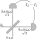
\includegraphics[draft=false, width=0.5\linewidth]{introduction/homodyne}
\caption{\label{fig:intro_homodyne} The homodyne detector mixes the mode to be measured, $\hat{a}_1$, with a strong local oscillator. The photocurrents are measured and subtracted $I_2 - I_1$, which gives measurement information about $\hat{q}_\theta$. The quadrature angle $\theta$ is controlled via the relative phase of the local oscillator.}
\end{figure}



\FloatBarrier
\subsection{Heterodyne measurement}
A heterodyne measurement scheme corresponds to the POVM
\begin{equation}\label{eqn:intro_heterodyne_povm}
\hat{\mathds{1}} = \frac{1}{2\pi} \int\limits_{\alpha \in \mathbb{C}} \Diff2 \alpha \; \dyad{\alpha}.
\end{equation}
The measurement gives outcome $\alpha$ with probability $(1/2\pi)\ev{\rho}{\alpha}$. This scheme may be realised as a ``double-homodyne'' protocol, in which an input state $\rho$ is split on a balanced beamsplitter, and conjugate quadratures $\hat{q}_1$, $\hat{p}_2$ are measured on different output arms. Since they operate on different modes, the operators $\hat{q}_1$, $\hat{p}_2$ must commute. Simultaneous measurement of conjugate quadratures on the \emph{same} mode cannot be performed with arbitrary accuracy, and so the heterodyne measurement outcomes must pay the penalty of increased variance in $\text{P}\left(q\right)$, $\text{P}\left(p\right)$. Physically this arises from mixing with $\rho$ with vacuum on the first beamsplitter.


The heterodyne detector allows us to consistently define a joint probability distribution of the measurement outcomes $q_1$, $p_2$. This function is known as the Hussimi $Q$ function and is a well-defined probability distribution on the phase space\footnote{Unlike others such as Wigner function or $P$ function, which we refer to only as quasi-probability distributions}. The Hussimi function corresponding to $\rho$ is thus
\begin{equation}
Q\left(q, p\right) = \frac{1}{2\pi} \ev{\rho}{\alpha} \qq{with} \alpha = \frac{q + i p}{\sqrt{2}}.
\end{equation}

\noindent In the main body of the Thesis we will speak of the heterodyne measurement as effectively giving two outcomes, $\qout, \pout$, one from each homodyned arm. The $\alpha$ required for Eq.~\ref{eqn:intro_heterodyne_povm} are then given by $\alpha = \left(\qout + i \pout\right)/\sqrt{2}$.





\FloatBarrier
\section{Entropy and probability}
We will introduce and discuss some quantum entropies which we will use in the first part of this Thesis. Quantum entropies are a marvellous and interesting area of quantum information theory, and there are many interesting similarities with and departures from classical information theory. Below we summarise some of the key results which we will make use of in this Thesis, and the reader is referred to Refs.~\cite{Nielsen2010, Tomamichel2016, Wilde2015, Watrous2019} for further information.



\FloatBarrier
\subsection{Conditional probabilities}
Let $X$ and $Y$ denote random variables, with their associated probability distributions $\text{P}\left(X\right), \text{P}\left(Y\right)$. The conditional probability of $X$ given $Y$, $\text{P}\left(X \given Y\right)$ measures the probability of event $X$, given prior knowledge of event $Y$. The probabilities $\text{P}\left(X\right)$, $\text{P}\left(Y\right)$ are known as the marginal probabilities, and are related to the conditional probability by summing over values of the prior $Y$:

\begin{equation}
\text{P}\left(X\right) = \sum_{Y=y} \text{P}\left(X \given Y\right) \text{P}\left(Y\right).
\end{equation}

\noindent Bayes' theorem may be used to relate conditional probabilities to each other:

\begin{equation}\label{eqn:intro_bayes}
\text{P}\left(X \given Y\right) = \text{P}\left(Y \given X\right) \frac{\text{P}\left(X\right)}{\text{P}\left(Y\right)},
\end{equation}

\noindent and we make extensive use of this formula in the first part of this Thesis.

\FloatBarrier
\subsection{Hoeffding's inequalities}
Let $\mathcal{X} = X_1, X_2, \dots, X_n$ be $n$ independent binary random variables. Let $\bar{\mathcal{X}}$ be their empirical mean and let $\mathbb{E}\left(\bar{\mathcal{X}}\right)$ be its expected value. Then $\forall \epsilon \ge 0$ we may bound the probability that the empirical mean $\bar{\mathcal{X}}$ differs from its expectation $\mathbb{E}\left(\bar{\mathcal{X}}\right)$ by the following inequalities:

\begin{align}
\label{eqn:hoeffding1}
\text{P}\left(\bar{\mathcal{X}} - \mathbb{E}\left(\bar{\mathcal{X}}\right) \ge \epsilon\right) &\le \text{exp}\left(- 2 \epsilon^2 n\right) \\
\label{eqn:hoeffding2}
\text{P}\left(\mathbb{E}\left(\bar{\mathcal{X}}\right) - \bar{\mathcal{X}} \ge \epsilon\right) &\le \text{exp}\left(- 2 \epsilon^2 n\right).
\end{align}



\noindent These inequalities are known as Hoeffding's inequalities \cite{Hoeffding1963} and will provide a necessary tool for analysis of our Quantum Digital Signatures protocol.



\FloatBarrier
\subsection{Shannon entropy}\label{sec:intro_shannon_entropy}
Let $X$ be a random variable, which takes values $X_1, X_2, \dots X_N$ with probability $\text{P}\left(X_1\right), \text{P}\left(X_2\right),\dots,\text{P}\left(X_N\right)$. The Shannon entropy associated with this variable is defined as 

\begin{equation}
H\left(X\right) = - \sum_{j=1}^N \text{P}\left(X_j\right) \log \text{P}\left(X_j\right).
\end{equation}

\noindent The Shannon entropy represents the degree of uncertainty which one possesses about the variable $X$. If the value of $X$ is known (minimum uncertainty) then\footnote{By convention we take $0 \log 0 = 0$.} $H\left(X\right) = 0$. Conversely, if all possible values of $X$ are equally likely (maximum uncertainty) then $H\left(X\right) = \log N$.

\FloatBarrier
\subsection{Binary entropy}
Let $X$ be a binary random variable, which takes value $0$ with probability $p$ and value $1$ with probability $1-p$. Then the binary entropy of $X$ is defined as

\begin{equation}
\text{h}\left(X\right) = - x \log x - \left(1-x\right) \log \left(1-x\right).
\end{equation}
The binary entropy is a special case of the Shannon entropy for a binary random variable. We display the binary entropy $\text{h}\left(X\right)$ in Fig.~\ref{fig:binary_entropy}.

\begin{figure}
\centering
\captionsetup{width=0.8\linewidth}
\includegraphics[draft=false, width=0.5\linewidth]{introduction/binary_entropy}
\caption{\label{fig:binary_entropy} The binary entropy $\text{h}\left(x\right)$ is bounded by $\log 2$.}
\end{figure}


\FloatBarrier
\subsection{Mutual information}
We define the joint entropy $\text{H}\left(X, Y\right)$ of two random variables $X$ and $Y$ as the Shannon entropy of the joint probability distribution $\text{P}\left(X, Y\right)$. 

The conditional entropy of $X$, conditioned on $Y$ is
\begin{equation}
\text{H}\left(X \given Y\right) = \text{H}\left(X, Y\right) - \text{H}\left(Y\right)
\end{equation}
which measures the average uncertainty we have about variable $X$ given that we know $Y$.

One may expand the conditional entropy as \cite{Wilde2013}
\begin{equation}\label{eqn:intro_conditional_entropy_expansion}
\text{H}\left(X \given Y\right) = \sum_{Y=y} \text{P}\left(Y=y\right) \text{H}\left( X \given Y=y \right),
\end{equation}
where the expansion is over particular outcomes of the prior variable. Equation~\ref{eqn:intro_conditional_entropy_expansion} admits a natural extension to the case when the prior variable is continuous rather than discrete, with $\sum_{y}$ replaced by $\int \mathrm{d}y$.


The mutual information between $X$ and $Y$ may be defined as

\begin{equation}\label{eqn:intro_mutual_information}
I\left(X : Y\right) = \text{H}\left(X\right) - \text{H}\left(X \given Y\right),
\end{equation}

\noindent which is a measure of how much knowledge of one variable reduces uncertainty of the other variable. The mutual information is symmetric in its arguments.


\FloatBarrier
\subsection{Von Neumann entropy}
The Von Neumann entropy of a quantum state $\rho$ is
\begin{equation}
\text{S}\left(\rho\right) = - \tr\left[\rho \log \rho \right],
\end{equation}
which may be equivalently calculated as
\begin{equation}
\text{S}\left[\rho\right] = - \sum_j \lambda_j \log \lambda_j,
\end{equation}
where $\lambda_j$ are the eigenvalues of $\rho$. The Von Neumann entropy is always non-negative, and is zero when $\rho$ is pure.

By analogy with the Shannon entropy we will additionally define the joint entropy of a composite system $\rho_{A, B}$ in the obvious way
\begin{equation}
\text{S}\left(\rho_{A, B}\right) = - \tr\left[\rho_{A, B} \log \rho_{A, B}\right].
\end{equation}

\noindent The conditional Von Neumann entropy between quantum systems $A$ and $B$ may then be defined
\begin{equation}
\text{S}\left(A \given B\right) = \text{S}\left(A, B\right) - \text{S}\left(B\right),
\end{equation}
where the Von Neumann entropy of a quantum system $A$ or $B$ should be understood as the entropy of the corresponding state $\rho_A$, $\rho_B$.


\FloatBarrier
\subsection{Holevo information}
The Holevo information $\chi$ is an upper bound on the mutual information $I$, and plays a crucially important role in many areas of quantum information processing. 

We introduce two players, Alice and Bob. Let Alice prepare a state $\rho_j$, $j = 1, 2, \dots, N$, with probability $p_1, p_2, \dots, p_N$. Bob wishes to distinguish whichof the $\rho_j$ Alice has prepared. 

Bob may perform any measurement described by POVM elements $\left\{E_K\right\}$, and he receives a measurement outcome $K$. Then the mutual information $I\left(j : K\right)$ describes the knowledge of which $\rho_j$ was prepared, given Bob's measurement outcome $K$. The mutual information us upper bounded by the Holevo information

\begin{equation}\label{eqn:intro_holevo_bound}
I\left(j : K \right) \le \chi \left(j : K \right),
\end{equation}
with the Holevo information $\chi$ defined as

\begin{equation}\label{eqn:intro_holevo}
\chi\left(j : K\right)  = \text{S}\left(\rho\right) - \sum_j p_j \text{S}\left(\rho_j\right),
\end{equation}
with
\begin{equation}
\rho = \sum_j p_j \rho_j.
\end{equation}

\noindent For a pleasing proof that $I$ is bounded by $\chi$ we refer the reader to Ref.~\cite{Nielsen2010}. 

Throughout this Thesis we will refer to the first term in Eq.~\ref{eqn:intro_holevo} as the \emph{a priori} entropy (with its corresponding \emph{a priori} state $\rho$), while we refer to the second term as the \emph{a  posteriori} entropy (with its corresponding \emph{a posteriori} state $\rho_j$). The bound in Eq.~\ref{eqn:intro_holevo_bound} will be used extensively in the cryptographic security proofs in the first part of this Thesis.


\FloatBarrier
\subsection{Conditioning cannot increase entropy}

A useful property of both Shannon and Von Neumann entropies is that ``conditioning cannot increase entropy.'' Quantitatively, we have for a quantum state $\rho_{A, B}$

\begin{equation}
\text{S}\left(A\right) \ge \text{S}\left( A \given B \right),
\end{equation}
where the entropy of system $A$ should be understood as the entropy of $\rho_A = \tr_B\left[\rho_{A, B}\right]$. Similarly, for classical random variables $X, Y$:
\begin{equation}
\text{H}\left(X\right) \ge \text{H}\left(X \given Y\right).
\end{equation}









%\part{Agile cryptography: signatures and secrets}
%\chapter{Introduction to quantum cryptography}\label{chapter:crypto_intro}

\section{Conventional (classical) cryptography}

Cryptography is a field probably as old as civilization itself. For as long as communication has existed, so too has the desire to keep information hidden. Both the Greeks and the Romans are known to have used ciphers to encrypt messages \cite{Singh2000}. A cipher, after applied to a message, allows the encrypted message to be freely transmitted and intercepted without an adverse party interpreting its meaning. The intended recipients, however, can undo the effects of the cipher and read the original message. 

One famous example is the Caesar cipher. In the Caesar cipher, each element of the alphabet which makes up the message (``plain'') is assigned a new symbol (``cipher''). Typically this is done by shifting the alphabet by a known quantity, Fig.~\ref{fig:caesar}. The plaintext message is encoded with the cipher, replacing letters from the plain with letters fromt he cipher. This encoded message is known as ``ciphertext'' and now may be freely distributed. At face value, the ciphertext is unreadable to anyone without access to the cipher.

\begin{figure}[htp]
\centering
\captionsetup{width=\linewidth}
\begin{framed}
\begin{align*}
\text{Plain:} &\text{  \code{ABCDEFGHIJKLMNOPQRSTUVWXYZ}} \\
\text{Cipher:} &\text{  \code{FGHIJKLMNOPQRSTUVWXYZABCDE}} \\
\text{Plaintext:} &\text{  I like physics} \\
\text{Ciphertext:} &\text{  N qnpj umdxnhx}
\end{align*}
\end{framed}
\caption{\label{fig:caesar} The cipher alphabet is formed of the plain alphabet shifted $5$ elements to the left. Knowledge of the cipher allows the plaintext message to be recovered.}
\end{figure} %TODO: change this to Hello to Jason Isaacs, or similar.
%TODO: put Hello to Jason, or similar, in my acknowledgements. It'll be banter.


Cryptanalysis -- the art and science of breaking cryptographic systems -- has existed for as long as cryptography, and history of cryptographic development can be viewed as an arms-race between cryptographers and cryptanalysts. The cryptographers, which we canonically call Alice and Bob, continually invent new schemes to perform their secure communication task. The cryptanalyst, which we canonically call Eve, continually tries to break these schemes in order to interfere in Alice and Bob's communication and obtain their messages. For example, the Caesar cipher can be broken by trying all possible shifts of the alphabet and checking which give a sensible message at the output. Against a more general cipher, Eve can perform a statistical analysis on the ciphertext, provided that she knows the language of the message. In English, for example, Eve knows that ``e'' is the most frequently occurring letter, and so the most common letter in the ciphertext is likely to decode to ``e''.

Many advances on the Ceasar cipher have been developed, in which a key (a shared secret piece of information) is used to encrypt and then decrypt a message. While many schemes are secure against decryption, they meet significant practical issues to actually distribute the key. Indeed, the key distribution problem was one of the longstanding and difficult problems which cryptographers have faced over the millenia. Should the shared keys fall into enemy hands, secret messages may be freely decrypted and their sensitive information made public. 

One practical method to distribute keys requires Alice and Bob to meet face-to-face, in advance of their communication, to share the keys which they will use for the next round of communication. While secure, this is impractical. A third party courier could be used as a go-between, but this places an assumption about the trustworthiness of the messenger, and requires an unweildly overhead for large-scale communications. In the second half of the $20^\text{th}$ Century, the following critical question became the focus of intense study of a small group of cryptographers: ``How can Alice and Bob share a secret key, without ever meeting each other?'' 

To solve this problem, Diffie and Hellman \cite{Diffie1976} required a fundamental paradigm shift to the structure of conventional encryption. Normally, as with the Caesar cipher, Fig.~\ref{fig:caesar}, the same key is used to encrypt and to decrypt the message, Fig.~\ref{fig:pubpriv} (a), a structure known as ``private-key (symmetric) cryptography''. We have seen that sharing this key becomes a weak link in the encryption protocol. Diffie and Hellman realised that it is possible to share the key without Alice and Bob ever meeting\footnote{Of course, at the beginning of the protocol Alice and Bob must be sure that they are actually talking to each other \cite{Shneier1996}.} face-to-face. The central idea behind the new ``public-key (asymmetric) cryptography'' was the existence of so-called \emph{one way} functions, which are easy to perform but difficult to invert. 

Diffie and Hellman's proposal runs as follows. At the start of communication, Alice and Bob publicly agree on a function $Y^x \text{modulo} P$, with $Y < P$. The $Y$ and $P$ are assumed to be public knowledge. For example, they may choose the function $f\left(x\right) 13^x \text{modulo} 19$. Now, Alice and Bob each choose a number, labelled $A, B$, and keep it secret, e.g. $A = 2$ and $B = 4$. Each number is fed into $f$: $\alpha :=f\left(A\right) = 17$ and $\beta := f\left(B\right) = 4$. The outputs $\alpha, \beta$ are shared between Alice and Bob; crucially, although calculating $\alpha, \beta$ was simple, it is tricky to find $A$ and $B$ from this public information. Finally, Alice calculates $\beta^A \text{ modulo } 19 = 16$ and Bob calculates $\alpha^B \text{ modulo } 19 = 16$: Alice and Bob reach the same number, $16$, which can then be used as the encryption key. This discovery allows Alice and Bob to establish a key entirely over public and insecure communication channels. 



\begin{figure}[htp]
\centering
\captionsetup{width=\linewidth}
\begin{framed}
\begin{subfigure}{0.4\textwidth}
\begin{align*}
m \mapsto \text{Encrypt}_\mathcal{K}\left(m\right) \\
\text{Decrypt}_\mathcal{K}\left[E_\mathcal{K}\left(m\right)\right] \mapsto m
\end{align*}
\caption{}
\end{subfigure}
\begin{subfigure}{0.4\textwidth}
\begin{align*}
m \mapsto \text{Encrypt}_\mathcal{E}\left(m\right) \\
\text{Decrypt}_\mathcal{D}\left[\text{Encrypt}_\mathcal{E}\left(m\right)\right] \mapsto m
\end{align*}
\caption{}
\end{subfigure}
\caption{(a) Private-key encryption. The same key $\mathcal{K}$ allows Alice to encrypt and Bob to decrypt message $m$. (b) Public-key encryption. Alice and Bob use different keys, $\mathcal{E}$ and $\mathcal{D}$ to encrypt and decrypt $m$. The key $\mathcal{E}$ can be public knowledge without affecting the security of the key $\mathcal{D}$.}
\label{fig:pubpriv}
\end{framed}
\end{figure}


Security of this key exchange system relies on the fact that $A$ and $B$ are kept secret, and it is the distinctions and relationships between public and private information which underpin public key cryptography. The function $f$ is sometimes referred to as a ``trapdoor'' or ``one-way'' function, and is typically based on a mathematical problem which is deemed to be computationally hard: that is, even the most powerful computers cannot hope to solve it in a feasible amount of time. Typically the time taken to solve scales exponentially in the size of the key. Perhaps the most well-known hard problem is that of factoring a large integer into primes, which underlies the commonly used RSA protocol \cite{Rivest1978, Schneier1996}.




This type of security, relying on assumptions about computing power, is known as \emph{computational} security. In principle these cryptosystems could be broken with a sufficiently powerful computer, or with algorithmic advances. It has been shown, however, that while these problems are hard for a classical computer, there exist algorithms for a future quantum computer which can break them. The most well known of these is Shor's algorithm \cite{Shor1997},  which provides an exponential speedup in the ability to split an integer into its prime factors. %nstead of taking an exponential number of steps in the length of the integer, the quantum computer will take a number of steps which is only polynomial in integer length. 
The existence of such algorithms which successfully solve the hard problems poses a threat to many commonly used cryptosystems %such as RSA, DSA and ECDHE 
\cite{Rivest1978, Schneier1996, Amiri2015, Nielsen2010, Shor1997}. One must therefore carefully consider how to respond to this threat posed by quantum computers. 

One solution will be to switch the underlying hard problem to a different class of problems, which even a quantum computer cannot solve. This is the approach adopted by the Post-Quantum Cryptography (PQC) community, whose aim is to design protocols based on problems for which no good quantum algorithm is yet known \cite{Bernstein2017, Chen2016, Gagliardoni2017a, Bernstein2009, Alagic2019, Chrome2016}. However, it is still an open question which problems a quantum computer can hope to solve%\footnote{It is even not yet known whether they can solve a larger class of problems than a classical computer}
, and so a premature implementation of a secure system based on a PQC hard-problem, may still be threatened by a quantum computer as new algorithms are developed. 

%In any case, it is clear that the currently implemented cryptographic systems must either be strengthened or replaced, and this may prove challenging. We will briefly discuss some of the challenges, and a possible solution which has gained traction among the conventional cryptography community in recent years, in Chapter~\ref{chapter:aqc}

The second solution to the threat posed by quantum computers is to begin to adopt cryptosystems which are provably secure against a quantum computer. There exist classical protocols for which this is possible \cite{Shamir1979, Blakley1979}, and we will discuss some of them in Sec.~\ref{sec:qss_lit_review}. However for many applications classical cryptography does not allow for such provably secure systems without an initial face-to-face interaction\footnote{To facilitate, for example, the sharing of large, random, secure keys.}, and so one must move to the quantum realm.

Quantum cryptography bases its security not on the assumption of a mathematical problem's difficulty, but on physical laws. Instead of aiming for computational security (albeit security against a quantum computer), quantum cryptography aims to build the stronger \emph{unconditionally secure} (or \emph{information-theoretically secure}) protocols, which cannot be broken even in principle. By basing security on physical laws quantum cryptography requires the sharing of physical systems between players, and we shall see in the remainder of this Thesis that quantum light is a natural object with which to perform such cryptographic tasks. 

One may think of the advantage provided by quantum cryptography in terms of the one-way functions discussed earlier, Fig.~\ref{fig:qutrapdoor}. While the classical one-way functions are only computationally hard, the quantum analogue of the one-way function is provably impossible to invert. For example, if the unknown quantum states are chosen to be non-orthogonal then it is impossible to perfectly determine the classical information which they encode \cite{Nielsen2010, brendon_book}. Any malevolent party attempting to gain information will not do so perfectly, and will thus leave a detectable trace.

\begin{figure}[h!]
\centering
\captionsetup{width=\linewidth}
\begin{framed}
\begin{subfigure}{0.49\linewidth}
\begin{align*}
x_i &\mapsto f\left(x_i\right) \qq{easy} \\
f\left(x_i\right) &\mapsto x_i \qq{hard}
\end{align*}
\caption{}
\end{subfigure}
\begin{subfigure}{0.49\linewidth}
\begin{align*}
x_i &\mapsto \ket{x_i} \qq{easy}\\
\ket{x_i} &\mapsto x_i \qq{impossible}
\end{align*}
\caption{}
\end{subfigure}
\caption{(a) A classical one-way function $f$ is easy to perform but computationally difficult to invert. $f$ is typically based on a hard problem. (b) A quantum one-way function. If the quantum states $\ket{x_i}$ are chosen to be non-orthogonal then it is impossible to perfectly determine the classical information $x$, given a quantum state $\ket{x}$. This forms the basis for quantum cryptosystems, whose security is guaranteed by the no-cloning theorem \cite{Nielsen2010, brendon_book}}
\label{fig:qutrapdoor}
\end{framed}
\end{figure}

%\clearpage
\section{Quantum digital signatures protocols}
%This section will basically be my "literature review" section.
%I will focus on the main thread of QDS developments initially, but I can supplement it by including some of the asian papers later.

%Note: after I have this section I can compare it to the Amiri2015 review paper and to Collins2018 progress report (and to Callum's thesis)


\subsection*{Quantum one-way function}
%Talk about Gottesman and Chuang.
Gottesman and Chuang \cite{Gottesman2001} generalized Lamport's scheme \MT{cite} in $2001$ to build the first Quantum Digital Signatures protocol. The key contribution of their scheme is to replace the one-way function in \MT{cite} with a so-called \emph{quantum one-way function}, thereby securing the signatures protocol against a quantum adversary.

\MT{TODO: chat more about quantum one-way function. Include the "figure" that I currently have in my historical introduction}

A direct analogue of public-key cryptography, their protocol relies on the difficult task, described in Fig.~\MT{X}, of accurately distinguishing between non-orthogonal quantum states. Their security relies on the fact that performing measurement on a state of $n$~qubits can yield at most $n$~bits of information, and so the protocol in Ref.~\cite{Gottesman2001} is designed such that this is insufficient to distinguish between states.

The key tool in the protocol is a quantum $SWAP$ test, Fig.~\MT{X}, which probabilistically determines whether two states are identical. To perform this test, players prepare $\ket{f_x}, \ket{f_{x^\prime}}$ and an additional ancilla $\left(\ket{0} + \ket{1}\right)/\sqrt{2}$. Players perform a Fredkin gate \MT{cite} using the ancilla as a control, and then perform a Hadamard \MT{cite} on the ancilla. In other words, the $SWAP$ test performs the mapping
\begin{equation}
\ket{f_x}\ket{f_{x^\prime}}\frac{\left(\ket{0} + \ket{1}\right)}{\sqrt{2}} \mapsto \frac{\left(\ket{f_x}\ket{f_{x^\prime}} \pm \ket{f_{x^\prime}}\ket{f_x}\right)\ket{y_{\pm}}}{\sqrt{2}}
\end{equation}
with $y_+=0$ and $y_-=1$. Finally, the ancilla qubit is measured in the $0, 1$ basis, and since $\ket{0}, \ket{1}$ are orthogonal they can be distinguished.  Therefore if $x = x^\prime$ the coefficient of $\ket{1}$ is identically zero, and so the $SWAP$ test always outputs $\ket{0}$. If $x \ne x^\prime$ outputs either $\ket{1}$ or $\ket{0}$. 

The probabilistic nature of this test will cause participants in the protocol to sometimes mistake distinct states for identical ones, but the probability that this occurs may be estimated. Crucially, the protocol may be proven secure if states are chosen such that this probability of honest failure is smaller than the probability to correctly distinguish between large entangled states of non-orthogonal qubits. 

The protocol is a significant attempt to generalise and translate structures from the field of classical cryptography to the quantum realm, and it sets the pattern for all subsequent QDS protocols, and so it is worth examining the protocol in detail. Alice has a $1$~bit message $b$ which she would like to sign, and send to Bob and Charlie. In the Distribution state, for each $b$ Alice creates $M$ classical strings $k_m^i$, length $L$. Each classical string is mapped to a corresponding quantum state $\ket{k_m^i}$ of $n$~qubits which are chosen to be highly non-orthogonal. Two of each of these quantum states are sent to Bob and Charlie. The quantum states, $4M$ in total, are Alice's public keys which may be freely distributed--and they may even be given to a dishonest external party. The corresponding classical strings $k_m^i$ are Alice's private keys.

Bob and Charlie each receive two of the $\ket{k_m^i}$. They each perform a $SWAP$ test between their two copies of the public key, to check whether individual copies are equivalent. Then, they should perform a $SWAP$ test between one of Bob's keys and one of Charlie's keys, to test whether they received identical keys to each other. If all $SWAP$ tests pass then the protocol continues to the next step, otherwise it aborts. Bob and Charlie should now store the quantum public keys which they hold.

Later, in the Messaging stage, Alice sends $\left(m, k_m^i\right)$. For each of the $M$ strings $k_m^i$, Bob creates $\ket{k_m^i}$ and performs a $SWAP$ test with his corresponding stored quantum state. If his test passes most of the time then he accepts the message as genuine and transferable, and passes $\left(m, k_m^i\right)$ to Charlie who performs similar tests. 

Although laying the groundwork for practical QDS protocols, this original proposal cannot be implemented. The most pressing problem is the requirement for long-term quantum memory. State-of-the-art technology can store a quantum state for \MT{X}, and so long-term storage of many copies of quantum states with many qubits will be technologically challenging. Furthermore, the need for every party to be able to create and distribute the states and the multiple required $SWAP$ tests render this protocol impractical for implementation. 

However, as we shall see, the structure of this protocol is very closely aligned to classical signatures protocols. Since the public keys are truly public (all of them can be handed to Eve). Furthermore, every recipient is given identical quantum public keys and so the number of recipients does not need to be fixed before the start of the protocol. These requirements are subtly changed in later--more practical--QDS protocols. \MT{make sure I talk about this later.}

\MT{Perhaps talk about repudiation somewhere in this section?}

%\subsection{Andersson2006 (+ implementation)}
\subsection*{QDS implementation}
%Talk about Andersson2006 and Clarke2012
A step forward to implementation of QDS occurs in Ref.~\cite{Andersson2006}, in which Andersson \emph{et. al.} replace the tricky to perform $SWAP$ test from Ref.~\cite{Gottesman2001} with a practical state comparison method. The qubits required previously are also replaced by coherent states (qumodes). Combined with the new state comparison scheme, the requirements for QDS have been reduced to just generation and distribution of coherent states and linear optics components (beamsplitters).

\begin{figure}[htp]
\centering
\includegraphics{andersoon2006_state_comparison.png}
\caption{\label{fig:andersson2006_state_comparison}}
\end{figure}

The key step, the comparison of coherent states, is displayed pictorially in Fig.~\ref{fig:andersson2006_state_comparison}. If the photodetector clicks it is a strong indication (a certain indication, in the ideal limit) that $\alpha \ne \beta$. Furthermore this comparison is non-destructive, and simply by placing another beamsplitter in the path of the upper beam, with vacuum input at the fourth port, one recovers $\ket{\alpha}$. Otherwise, for $\alpha \ne \beta$ the output states of the second beamsplitter are identical. This practical state comparison forms the building-block for their QDS protocol. 

\begin{figure}[htp]
\centering
\includegraphics[width=0.8\linewidth]{multiport.png}
\caption{\label{fig:andersson2006_multiport}}
\end{figure}

To allow both parties to perform comparisons, an optical multiport Fig.~\ref{fig:andersson2006_multiport} is used. This allows Bob and Charlie to compare Alice's state declaration with her previously distributed state. It also has the advantage of symmetrizing Bob and Charlie's output states, thus preventing a repudiating Alice. The null ports of the multiport are monitored, since they will click if either Alice is trying to repudiate, or if a malicious party is interacting with the state distribution.

Alice sends coherent states from her alphabet of possible coherent states, both to Bob and to Charlie, and keeps a record of which states she sent. Bob and Charlie feed their states through the shared multiport, thereby ensuring that Alice has sent them identical states (or symmetrizing them if she hasn't), and store their output states in quantum memory. Later, Alice sends the classical message, plus classical information describing which states she had previously sent. Bob and Charlie create the corresponding coherent states, and compare them via the method in Fig.~\ref{fig:andersson2006_state_comparison} with the states retrieved from quantum memory. If no clicks are recorded at the null ports, it is an indication that the message is genuine and the protocol passes.

This protocol was implemented by Clarke \emph{et. al.} in Ref.~\cite{Clarke2012}, where an alphabet with $8$ phase-encoded coherent states was used, and signature lengths $L \sim $\MT{X} were obtained. \MT{I don't think they actually quote one, but I can estimate it from their $g$ value.} To get around the requirement for quantum memory, in Ref.~\cite{Clarke2012} the Messing and Distribution stages occur at the same time so the coherent state corresponding to the chosen private key may be interfered with the distributed quantum signatures. This prevents their scheme from being used in a realistic setting where the Distribution and Messaging stages can typically occur with a delay of days, weeks or even years.




%\subsection{Dunjko2014 (+ implementation}
\subsection*{Removing quantum memory}
The requirement that recipients possess long-term and efficient quantum memory, needed for the above protocols, makes it impractical for realization. The removal of this requirement by Dunjko \emph{et. al.} \cite{Dunjko2014} was one of the major milestones towards a practical QDS which can be implemented. 

The key insight of Ref.~\cite{Dunjko2014} was to effectively replace the quantum public key by a classical one, albeit one which relies on the distribution and measurement of non-orthogonal quantum states. This physical requirement is a practical one, relying on simply linear optics (beamsplitters) and photodetectors capable of distinguishing just between zero and nonzero photon numbers, such as avalanche photodiodes (APDs). The storage of classical public keys is clearly no restriction. 

The main difference then between Refs.~\cite{Dunjko2014} and \cite{Gottesman2001}, is that in Dunjko \emph{et. al.}, recipients Bob and Charlie perform photon-number measurement as they receive the quantum states. Remarkably, despite this fundamental change to the nature of the protocol's one-way function, secure QDS is possible. \MT{do I need to revise this sentence? Is it accurate and fair?}

\MT{Include a figure (minipage thing) comparing the one-way functions used by Gottesman2001 and by Dunjko2014.}

In the Distribution stage of the protocol, Alice generates classical strings $\left\{k_j^m\right\}_{j=0}^L$, length $L$, corresponding to each future one-bit message $m$. The $k_j^m$ are chosen uniformly at random from the BPSK alphabet of coherent state phases $\left\{- \alpha, \alpha\right\}$. Alice then forms sequences of coherent states $\rho = \otimes_{j=0}^L \ket{k_j^m}$ which she then distributes to Bob and to Charlie. 



Bob and Charlie pass their received coherent states through the shared optical multiport, Fig.~\ref{fig:dunjko2014_multiport}, which serves to symmetrize their individual quantum states. That is, after the multiport Bob and Charlie's reduced density matrices are identical, which guards against Alice's repudiation attack. Each recipient has two outputs of the multiport. One output, the so-called "null-port" should be monitored for clicks of the photodiode which imply that $\alpha \ne \beta$ (Bob and Charlie have different coherent states, Fig.~\ref{fig:dunjko2014_multiport}) which may imply the presence of an attack. Bob and Charlie should also perform unambiguous state discrimination (USD) on the outputs of their signal ports, which will accurately distinguish between non-orthogonal states $\ket{\alpha}, \ket{-\alpha}$ at the expense that it will sometimes fail to give an answer. 

During Messaging, Alice will declare $\left(m, k_j^m\right)$ which recipients will compare to their USD outcomes. Provided that there are enough matches between Alice's phase declarations $k_j^m$ and Bob/Charlie's USD outcomes, message $m$ is accepted and the protocol has succeeded.

This first protocol avoiding the requirement for quantum memory shows that QDS may be both practical and secure. Furthermore the limited physical requirements--tensor-products of coherent states, beamsplitters and non-photon-number-resolving detectors--are feasible to work with, unlike the large number of superposition qubits required for Ref.~\cite{Gottesman2001}. \MT{Now talk about the implementation paper}. 

An implementation of a variation of Dunjko's scheme is described in Ref.~\cite{Collins2014}. Collins \emph{et. al.} modify Dunjko's scheme in two key ways. Firstly, a QPSK alphabet Eq.~\MT{X} is used, rather than BPSK. This is in order to make the second modification: instead of using unambiguous state discrimination (USD) measurement, they perform unambiguous state \emph{elimination} (USE) measurement. If the measurement succeeds, rather than being able to say definitively which state was received, a recipient can say with certainty which state was \emph{not} received. This measurement scheme is described further in Fig.~\ref{fig:USE}. The key advantage of the USE measurement scheme is that the probability that the measurement fails is significantly smaller than for USD, and so the resulting QDS scheme gains a boost in efficiency. Indeed, if USE eliminates $N-1$ of $N$ possible states then one knows with certainty which state was sent, USD may be viewed as a special case of the more general USE measurement. The shift from state discrimination to state elimination allows for much greater efficiency in QDS schemes. \MT{Make sure to talk about it later in the context of our QDS - make a graph showing $g$ (or $L$?) under discrimination vs elimination.}

\begin{figure}[htp]
\centering
\includegraphics[width=0.8\linewidth]{USE.png}
\caption{\label{fig:USE}}
\end{figure}

Collins \emph{et. al.} estimate a signature length $L = 5.1 \times 10^{13}$ in order to sign a message. Notice the subtle shift between Refs.~\cite{Gottesman2001} and \cite{Andersson2006, Clarke2012, Dunjko2014, Collins2014}. While previously the number of recipients did not need to be determined until the Messaging stage, here it must be determined before Distribution. After the coherent states have passed through the multiport the number of recipients cannot be changed. 
\MT{I should note later that removing the multiport removes this restriction.} Because of the physical requirements for the optical multiport, it will also be challenging (though possible) to generalize to more recipients, though note that for more than two recipients in Ref.~\cite{Dunjko2014} one may not use $USD$ measurement. \MT{why?}. Realistic implementation of the multiport also introduces noise and losses due to misalignment and instability, further reducing the efficiency of the protocol, and requires Bob and Charlie to be physically connected. In Ref.~\cite{Clarke2012, Collins2014}, for example Bob and Charlie are separated by $5$~m of optical fibre. 

The most difficult assumption which Refs.~\cite{Clarke2012, Dunjko2014, Collins2014} make, however, is that there should be no eavesdroppers on the quantum channels. This is a strong and impractical assumption, and one which subsequent papers endeavour to remove.

\subsection*{Removing multiport}
%\subsection{Wallden2015 (+ implementation)}

The fact that the QDS schemes discussed above require dedicated hardware at the receivers--the optical multiport--makes implementation in real-world situations difficult. The multiport introduces losses and noise, and requires tricky synchronisation between Bob and Charlie in order to correctly interfere the states. The experiment in Ref.~\cite{Collins2014} therefore has Bob and Charlie only separated by $5$~m optical fibre. 

To combat this, Wallden \emph{et. al.} \cite{Wallden2015} propose two QDS schemes specifically designed to run over the same hardware platform as QKD. In particular, they get rid of the multiport which was previously use to symmetrize Bob and Charlie's reduced output states. Their key insight is that rather than symmetrizing their states, it is sufficient to symmetrize their measurement outcomes. Therefore, a step is added to the distribution stage in which Bob and Charlie randomly swap half of their measurement outcomes over a secure classical channel. If Alice can gain no information about which outcomes were swapped then she cannot repudiate. 

This protocol was implemented by Donaldson \emph{et. al.} in Ref.~\cite{Donaldson2016} in which a message is securely signed over distances $500$~m, $1000$~m, and $2000$~m, with no requirement on the physical separation between Bob and Charlie. The secure classical link may be realised via QKD, and so Refs.~\cite{Wallden2015, Donaldson2016} begin to explore the close connections between these two different quantum communication protocols. We explore this further in Chapter.~\MT{X}. Donaldson \emph{et. al.} achieve signature length $L = 1.93 \times 10^9$ using QPSK coherent states and USE measurement. This is a vast improvement over the $L = 5 \times 10^{13}$ required in Ref.~\cite{Collins2014} and means that secure quantum signatures may actually be both useful and practical. 

\subsection*{Allowing Eve}
%\subsection{Amiri2016 (+ implementation)}
All signature schemes considered so far have made the assumption that the quantum distribution channels are secure, that is, they may not be attacked or monitored by an eavesdropper, Eve. This is clearly an unrealistic and unphysical assumption, but was a sensible one while the pressing impracticalities of early QDS schemes (quantum memory, multiport, tricky state comparison tests) were overcome. The emphasis in earlier papers was on dishonesty internal to the protocol, i.e. which attacks can Bob or Charlie mount when they already hold perfect copies of the quantum public keys. However, in a realistic scenario it is clear that an eavesdropper \emph{could} attack the quantum channels as states are being distributed, and so it is important to consider whether this has any effect on QDS security.

Amiri \emph{et. al.} provide a QDS scheme which allows for an Eve to eavesdrop on the quantum channels. In the worst-case scenario it is assumed that Eve will conspire with a dishonest internal player (Bob or Charlie in the case of a forging attack), and so knowledge which Bob/Charlie hold about their own quantum public key measurements is supplemented by knowledge learned through Eve's attack. For short, we describe Bob or Charlie as performing the eavesdropping attack, so as not to confuse the nomenclature. 

The key modification which Ref.~\cite{Amiri2016} makes is to have Alice use \emph{different} private keys (and so different sequences of quantum coherent states) for each recipient. This means that the dishonest recipient is forced to eavesdrop on the honest recipient's quantum channel if he is to gain any information. This is in contrast to earlier protocols in which the dishonest recipient held a perfect copy of the quantum public key, which was identical to that of the honest recipient. 

Because the dishonest player is forced to eavesdrop, he in fact receives a worst copy of the honest player's public key than in the above protocols, and so somewhat counter-intuitively Ref.~\cite{Amiri2016} requires \emph{shorter} $L$ than previous protocols, despite relaxing a security assumption. The protocol relies on sending weak attenuated coherent states, identically to decoy-state BB$84$ \MT{cite}, and \MT{X} detection at the receiver. Because the security of discrete-variable QKD is so advanced, the QDS protocol proposed in Ref.~\cite{Amiri2016} is secure against coherent eavesdropping attacks.\footnote{We will discuss the hierarchy of eavesdropping attacks in Sec.~\MT{X}}

\subsection{Side-channel attacks}
%\subsection{Puthoor2016 (+ implementation)}
%\MT{Though first talk about side-channel attacks}
It should be noted that "security" of a protocol is a theoretical statement, and not a physical one. A protocol is secure with respect to a model of how it operates in the real world, and whether a so-called unconditionally secure protocol can be broken in practice depends on how realistic or practical its underling modelling assumptions are. For example, although in many QKD protocols Eve is allowed to attack the quantum channels and eavesdrop on all communication, she is prevented from attacking the physical devices which are used to implement the protocol. 

For example, the QDS scheme presented in Ref.~\cite{Amiri2016} relies on distribution and detection of quasi-single photons \MT{make sure I have discussed this earlier} in different polarization bases. Physically, Alice must prepare her states before they are sent. A realistic Eve could attack Alice's device in order to gain information about the polarization of the prepared state and so she might gain enough information to forge without detection, even though the protocol is unconditionally secure against conventional types of eavesdropping attack.

An example of such a side-channel attack \MT{define what is a side-channel attack} is the trojan horse attack presented in Ref.~\cite{Jain2014}. Here, Eve shines a bright laser pulse into Alice's device and measures the few back-reflected photons which are scattered back. These photons have picked up the same polarization as Alice imparted to her prepared state, and so Eve is able to infer the chosen polarization basis choice, which gives her an undetected advantage.

To guard against side-channel attacks, honest parties have several options. One direction is to close known side-channels by additional protocol steps or additional hardware. For example, with the trojan horse attack Alice and Bob could add additional filters to their devices to block out light at Eve's required wavelength. It was shown however that Eve can bypass this by breaking Alice's filters, in a way that is undetectable to honest players \MT{cite the laser damage paper}. Closing side-channels in this way may open up the protocols to additional attack methods, which must then be understood, modelled and reacted-to. This places quantum cryptography into the same "cat-and-mouse" development cycles as conventional cryptography. \MT{expand on this, and make sure I have discussed it earlier in the historical overview.}

To break this cycle, and to provide genuinely unconditional security, guaranteed against all conceivable side-channel attacks, there has been a recent push towards device-independent cryptography. The security of device-independent (DI) protocols makes no trust assumptions about the devices used and it may even be assumed that the  devices are held by the malevolent party. DI cryptography is then based entirely on laws of quantum mechanics, specifically on the violation of a bell inequality. \MT{cite some stuff, and expand this paragraph.}

Full DI cryptography, while secure, is difficult to perform and may offer figures of merit which are too pessimistic for the desired application. One may compromise, then, and instead implement measurement device independent (MDI) cryptographic protocols, in which no trust assumptions are placed on the measurement devices (and they can even be owned by Eve), while the state-preparation and sending devices are held by honest parties and are trusted. \MT{cite some papers}

The first MDI QDS scheme is presented by Puthoor \emph{et. al.} in Ref.~\cite{Puthoor2016}.



\subsection{Tokyo installed fibers scheme}
\MT{Perhaps the rest of the DPS-based protocols, or installed-fiber protocols here too?}





\subsection{The other "almost-agile" ones?}

\subsection{An2019 (+ implementation)}

\subsection{Croal2016}
\MT{Discuss DV vs CV first}

\subsection{Quick chat about my PRA}
\MT{perhaps I just want to mention this in the "abstract"/introduction of this chapter? I don't want to talk about it too much because it is what the rest of the chapter is about.}


\subsection{"Classical" unconditionally secure signatures}
\MT{Talk about protocol P2 from Wallden2015, and also Amiri's scheme}

\subsection{Extensions to signature schemes}



\section{How to share a secret}\label{sec:qss_lit_review}
A secret sharing scheme allows for secure splitting and distribution of classical information among multiple recipients, an unknown subset of whom may be dishonest. The the canonical example of such a scheme is that of a bank. The head of the bank, Alice, wishes to distribute keys to the vault between several potentially untrusted deputies. If the deputies work together and use their keys simultaneously they are able to access the vault, but any nefarious deputies working alone should not be able to gain access.


%\MT{Make sure to cite the paper "how to share a secret" and talk about its title}.


\subsection{Classical secret sharing}\label{sec:qss_qcss}
Although many existing classical secret-sharing schemes are already information-theoretically secure \cite{Shamir1976, Blakley1979}, they may encounter problems when distributing  shares of the secret across insecure channels. This is analogous to the classical unconditionally secure signature schemes \cite{Wallden2015, Amiri2015a} discussed in Sec.~\ref{sec:lit_review_qds}, which implicitly required an underlying QKD encryption. Thus we may ask whether it is more or less resource-efficient to first run pairwise QKD between players, or to run a ``direct''-QSS scheme without first distilling pairwise secret keys. We should expect interesting parallels between QSS and QKD, since intuitively they are very similar, both effectively performing encryption of classical messages.

Let us consider some examples. Alice wishes to share a secret, $m$, between $n$ players, such that any $k \le n$ of them can access $m$. The general framework for this is called an $\left(n, k\right)$-threshold scheme, where of the $n$ players any subset of $k$ players can reconstruct the secret. An information-theoretically secure threshold sharing scheme was designed by Shamir in Ref.~\cite{Shamir1976}. Shamir's scheme relies on polynomial equations over finite fields, and is provably secure even against an adversary with infinite computing power. 

For example, Alice wishes to distribute a secret $m$ between four players, such that any three of them can access $m$. Alice generates a prime number $p$, and the polynomial 
\begin{equation}
\left( a x^2 + b x + m \right) \qq{modulo} p.
\end{equation}
Prime $p$ should be chosen larger than any of the coefficients $a, b$ or $m$. Alice then evaluates this polynomial at $4$ different points $x$, and sends the outcomes to each player. These points will be referred to as ``shares". %https://crypto.stackexchange.com/questions/9295/why-does-shamirs-secret-sharing-scheme-need-a-finite-field explains why a finite field is needed.
% It does need to be a field (integers aren't). Also it being finite means we can actually do the protocol.

The polynomial has three unknown coefficients, $a$, $b$ and $m$, and so any three players can combine their shares to create three equations, which may be solved for each unknown. Any fewer points will yield an underdefined system which cannot be solved. An attempt to guess the final share will show that any message $m$ can be the secret, and so such a guessing attempt is useless.

Another threshold secret sharing scheme was built on similar principles by Blakley \cite{Blakley1979}. In this scheme, the message $m$ is defined as a point in a large $k$ dimensional space. Each share is then a hyperplane in a $k-1$~dimensional space, which includes the point $m$. It therefore requires the intersection of all $k$ hyperplanes to reveal $m$. For example, if Alice again wishes to share a secret between four players, such that three of them are able to access $m$, then each share is a two-dimensional plane. The intersection of any two planes is a one-dimensional line containing $m$, and the third plane is required to reduce this line to the point $m$.

While both of these schemes are information-theoretically secure once the shares have been distributed (assuming that each share is securely stored and cannot be stolen), the main issue arises when considering how the shares can be distributed in the first place. If a malevolent party can access the shares during distribution then they can reconstruct the secret. In implementation, Shamir's and Blakley's schemes are therefore only as secure as the underlying encryption which is used to share the shares.

%\subsection*{Early quantum secret sharing}
%\MT{Gottesman1999, Karlsson1999, Hillery1999, Cleve1999}
%
%\MT{distinguish between secret sharing and state sharing}

\subsection{Quantum secret sharing}
We therefore wish to investigate whether the task of secret sharing can be made secure using quantum resources. It is important to notice that the translation from classical secret sharing to quantum secret sharing is not straightforward, and there are at least three directions which one can pursue:

\begin{itemize}
\item quantum-assisted classical secret sharing (qCSS): encrypt a classical secret sharing protocol \cite{Shamir1976, Blakley1979} using quantum resources. For example, perform pairwise QKD between Alice and each recipient, then encrypt the shares of the classical secret sharing protocol. This is analogous to the classical unconditionally secure schemes discussed earlier.
\item quantum secret sharing (QSS): use quantum states to securely distribute shares of a classical secret.
\item quantum state sharing (QStS): securely distribute shares of a quantum state.
\end{itemize}

Quantum state sharing is an important and exciting research direction in its own right and helps to establish the close links between quantum secret sharing, QKD and quantum teleportation \cite{Braunstein1998, Hillery1999, Markham2008a}. Despite the fact that both QSS and QStS are natural extensions of classical secret sharing to the quantum realm, and despite the fact that early work \cite{Hillery1999} proposes related protocols for each task, it should be understood that they are distinct quantum tasks with different goals and hardware requirements. For the rest of this Thesis we will restrict ourselves to QSS. In what follows we will only refer to the first two options as ``quantum secret sharing'', while the third option we shall refer to as ``quantum state sharing''.

\subsection{Entanglement-based QSS}


All three directions, qCSS, QSS and QStS are discussed at length in the pioneering work by Hillery \emph{et. al.} \cite{Hillery1999}. They propose the use of a GHZ resource state
\begin{equation}
\ket{GHZ} = \frac{1}{\sqrt{2}} \left(\ket{000} + \ket{111} \right)
\end{equation}
shared between three players, which can be used to distribute shares of a classical secret. Collaborating recipients can recover the secret while a dishonest subset of players cannot. Alternatively, the GHZ resource state may be used to distribute shares of a quantum state, such that collaborating players may reconstruct the original quantum state while a dishonest subset of players can gain no information.

For QSS, each player chooses independently and at random to measure their state in either $x$ or $y$ basis:
\begin{align}
&\ket{\pm x} = \frac{1}{\sqrt{2}} \left( \ket{0} \pm \ket{1}\right), \notag \\
%
&\ket{\pm y} = \frac{1}{\sqrt{2}} \left( \ket{0} \pm i \ket{1} \right). \notag
\end{align}
If, for example, all three players measure in the $x$ basis, then Charlie can infer from his measurement outcome whether Alice and Bob's measurements are correlated or anticorrelated. By collaborating, then, Bob and Charlie can accurately and securely infer Alice's bit. In fact, whenever Alice and Bob measure in the same basis as each other, Charlie must measure in $x$ in order to gain information. Conversely, if Alice and Bob measure in opposite bases then Charlie must measure in $y$, otherwise he gains no information. We see, then, that since each player randomly chooses which basis to measure, $50\%$ of the resource GHZ states will yield no information, and are effectively discarded.

Despite its high resource requirement, and despite the fact that $50\%$ of the resource states are wasted, Hillery's protocol has influenced the direction of all subsequent QSS protocols, and the paper was instrumental in demonstrating that multipartite entanglement is an important resource for quantum communication protocols. 
%\MT{Should I talk somewhere about qCSS in HBB paper?}
Multipartite entanglement is difficult to create and manipulate, and will degrade quickly as it is distributed over a quantum channel exposed to realistic loss or noise levels. Just as QKD has an equivalence between entanglement-based and prepare-and-measure versions \cite{Grosshans2003, Laudenbach2017}, it should be expected that the requirement of large multipartite state in Ref.~\cite{Hillery1999} can likewise be reduced \cite{Karlsson1999, Tittel2001, Zhang2005b, Williams2019}. 

To accomplish this, Karlsson \emph{et. al.} \cite{Karlsson1999} propose an entanglement-based QSS scheme which, rather than relying on creation and distribution of the GHZ state, relies on distribution of \emph{pairs} of entangled qubits in a Bell state. This configuration allows for correlations between players to be established identically to Hillery's scheme, but with more readily accessible resources. Recipients Bob and Charlie can determine with certainty which Bell state Alice sent, which allows Alice to establish a key with Bob/Charlie, and which may subsequently be used to encrypt a message. %\MT{demonstrate that it can give the same measurement outcomes as HBB with GHZ.}

This protocol drastically reduces the requirements of practical QSS, but the resulting protocol is still tricky to implement. The protocol requires Bell states and superpositions of Bell states, which will degrade over a realistic channel.  The protocol also introduces a fundamental asymmetry into QSS at the quantum level. While in Hillery's protocol protocol any of the three players can be chosen as dealer, for Ref.~\cite{Karlsson1999} it is established at the time of quantum state distribution that Alice is dealer. % which may make the protocol require bespoke hardware.

Both the protocols from Hillery \cite{Hillery1999} and Karlsson \cite{Karlsson1999} assume perfect state creation and noiseless and lossless quantum channels. This is an unrealistic assumption and one which must be relaxed before entanglement-based QSS can be implemented securely. 

Chen \emph{et. al.} \cite{Chen2005a} modify the Hillery's protocol \cite{Hillery1999} to allow for an imperfect distribution of entangled state. By proposing a method for entanglement distillation on a multipartite state, which can be used before a cryptographic protocol, Chen effectively reduces the extreme resource requirement of protocols like Ref.~\cite{Hillery1999}. The resource state does not even need to violate a Bell inequality.

An important generalization of the Hillery's scheme allows for analysis of the optimal entangled states required to share a secret between more than three players. While one option would be to simply replace the resource state with the N-partite GHZ state

\begin{equation}
\ket{N-GHZ} = \frac{1}{\sqrt{2}}\left(\ket{000\dots0} + \ket{111\dots1} \right)
\end{equation}

\noindent another option is to generalize to graph states \cite{Markham2008a, Keet2010} or in the continuous-variable regime Refs.~\cite{Lau2013, Wu2016} under which the tasks qCSS, QSS, QStS and entanglement-based QKD may be united and described within the same framework. %A graph state is a special type of multipartite entangled state.
One advantage of using such a state is that it can allow for QSS to be completed without collaboration from all recipients, which may help practical QSS to be robust and prevent against denial-of-service attacks from a dishonest internal player\footnote{Though we note that even QKD is susceptible to denial-of-service attack where Eve simply destroys the quantum (or classical) channels between Alice and Bob.}.

There have been several attempts to prove security of entanglement-based QSS. As we have seen, security proofs based on highly-entangled GHZ states or graph states become insecure once realistic channel parameters are considered, even though they offer unconditional security in the ideal limit. One way to tackle this is to borrow tools from entanglement-based QKD. Kogias \emph{et. al.} use similar analysis to so-called one-sided device-independent ($1$sDI) QKD \cite{Walk2016, Armstrong2015} in order to prove QSS security while modelling channel effects on their CV resource state.

Key to Kogias' protocol is the assumption that neither the measurement device of Bob, nor of Charlie, should be trusted. Rather, each player is assumed to possess a black-box which can output one of two measurement outcomes, corresponding in the honest case to homodyne measurement in either $x$ or $p$ quadrature. Protocol security is based on monogamy of entanglement and employs an entropic uncertainty relation which makes no assumption about the action of a dishonest player.. To our knowledge Ref.~\cite{Kogias2017} marked the first full security proof of QSS, against all forms of dishonesty and all types of attack over realistic channels. It was later shown that the resource required for entanglement-based QSS is two-way steering of the shared state \cite{Xiang2017, Xiang2018}, where the optimal Gaussian resource states for a given energy were also considered. 

The links between QSS and $1$sDI QKD explored in Ref.~\cite{Kogias2017} hint at an interesting direction for exploration: what is the relationship between QSS and other quantum communication protocols? It was already shown in Ref.~\cite{Markham2008a} that qCSS, QSS and QStS may be united under the same framework using graph states, while even in Hillery's oroiginal work \cite{Hillery1999} the links between qCSS and QSS were acknowledged. Additionally it can be shown \cite{Hillery1999} that a QStS protocol may be readily constructed from a teleportation protocol plus QSS (or qCSS or QKD) scheme if Alice teleports a quantum state to Bob, but sends the classical information required for state reconstruction to Charlie.

There are strong links between QSS and quantum conferencing \cite{Wu2016, Ottaviani2017b} which is a natural multipartite generalization of QKD in which $N$ players receive identical keys. Indeed, as shown in Refs.~\cite{Wu2016, Ottaviani2017b} the same resource states and network configurations may be readily used for both QSS and quantum conferencing. It is an open question however whether these additional tasks have the same optimal requirements \cite{Kogias2017, Xiang2017} on the resource state as QSS. %, or whether the optimal resource state for one protocol remains optimal for another protocol. 


%\MT{Add some more detail to this section. Add some examples of states and the transformations on them, and how they are used for QSS. Add some pictures too.}

%\MT{Add some chat about experimental implementations of EBQSS.}

%\MT{Still got some papers I need to talk about.}

\subsection{Sequential QSS}
The above protocols which implement QSS using entangled resource states offer an advanced level of security and neatly demonstrate the important role of entanglement in quantum communication. However, it is hard to see how they will be preferable to qCSS which can offer equivalent levels of security for the same task, but without the problems associated with generation and distribution of large entangled states. An entanglement-based scheme may even be fine if the number of players is small -- for example the scheme \cite{Karlsson1999} relyies only on Bell-pairs -- they cannot be easily scaled to many parties. We note that qCSS scales much more favourably as the number of required quantum channels is linear in the total number of players.

It should still be explored whether there are any QSS protocols which outperform qCSS. One promising direction is that of sequential\footnote{Sometimes referred to as entanglement-free QSS.} QSS in which the QSS task is fulfilled by sharing of a single quantum system between multiple players.

In the first sequential QSS protocol \cite{Zhang2005}, Zhang \emph{et. al.} propose a system in which Bob prepares a single photon state with his choice of polarization and sends it to Charlie. Charlie performs a unitary operation, either the identity, a Hadamard gate or a bit-flip, on the photon and sends it to Alice who stores the photon in a quantum memory. This process is repeated many times. Later, Alice will sample some of her stored photons for errors by asking Bob and Charlie to declare which state was sent and which operation was performed. She then performs the claimed operation, and measures the claimed basis, in order to check for errors.

On the remaining photons Alice performs her unitaries (either the identity or a bit-flip) to encode her secret. She then sends the photons back to Charlie. %\MT{how does the rest of the protocol run?}
If Bob and Charlie collaborate they can deduce the correct basis in which to measure Alice's photon, and so recover her information.



Sequential protocols have the obvious advantage that large entangled states are not required. Even though Ref.~\cite{Zhang2005} proposes to use a quantum memory it is ultimately not necessary for the protocol, and the work by Schmid \emph{et. al.} demonstrates this in a sequential QSS experiment \cite{Schmid2005}. Their experiment, in which players perform operations on heralded single photons, allows for a secret to be shared among six players in a setup which is much more readily scalable to more players than the earlier QSS schemes requiring entanglement.

\MT{Describe and appraise Schmid's protocol.}

Schmid's scheme relies on sequential interactions with a qubit state encoded into the polarization of a heralded single photon. Each player imposes a randomly chosen phase onto the state
\begin{equation}
\frac{\ket{0} + \ket{1}}{\sqrt{2}} \rightarrow \frac{\ket{0} + e^{i \phi_k} \ket{1}}{\sqrt{2}}
\end{equation}
and so at the end of the distribution the state is
\begin{equation}
\frac{\ket{0} + \exp\left(i \sum_{k}^N \phi_k\right)\ket{1}}{\sqrt{2}}.
\end{equation}
The final player measures in the $\ket{0} \pm \ket{1}$ basis. Collaboration of the first $N-1$ players allows them to infer, with certainty, the $N^{\text{th}}$ player's outcome.


%Just as prepare-and-measure QKD allows Alice and Bob to mimic the measurement outcomes of a shared entangled state  under \MT{criterion} the scheme \cite{Zhang2005} allows players to receive the same measurement outcomes they would if they had shared a GHZ state. Secret sharing then may proceed in the usual way. \MT{talk about this.}

The sequential scheme, while secure against an Eve external to the protocol, is difficult to secure against dishonesty from one of the internal players \cite{Deng2005, Qin2006, He2007}. For example, Ref.~\cite{He2007} points out that the order in which recipients declare their information is of utmost importance, and this is adopted into the sequential protocol in Ref.~\cite{Schmid2007}. Unfortunately, the protocol remains insecure against a so-called Trojan Horse attack \cite{Deng2005}, in which an internal player to the protocol adds one mode of an entangled state to the single photon as it is being distributed. This entangled mode will undergo the same subsequent gates as the signal photon, and so the dishonest player gains additional information. 

The Trojan Horse attack is guarded against in the recent work from Grice \emph{et. al.} \cite{Grice2019}. In their protocol for sequential QSS, each player creates a coherent state which is chosen from a Gaussian modulation. These states are added to the initial coherent state as it travels, and the final state is heterodyned by the dealer, Alice. With combined knowledge of their injected states, the players are able to estimate Alice's measurement outcome. This protocol has the advantage of high tolerable losses, especially when compared to entanglement-based QSS. Crucially, the scheme is immune to Trojan Horse attacks since once a coherent state has been added to the total state, it only interacts with Alice's measurement apparatus and does not pass through the equipment of any other player. Additionally a dishonest player cannot access other players' devices.

Owing to its simplicity of implementation QSS has been performed in many experiments \cite{Schmid2005, Hai-Qiang2013a} including those explicitly using telecom fiber networks \cite{Bogdanski2009}. This latter work, Ref.~\cite{Bogdanski2009}, demonstrates QSS in two experiments between three players and four players using phase encoding of single qubits. Their implementation uses a Sagnac interferometer, with light travelling in two directions around a loop. The light is at standard telecom wavelengths $1550$~nm and channel lengths are between $50$ and $70$~km, rendering secure QSS eminently practical.


\subsection{Summary}
Quantum Secret Sharing has been an intense field of active research for the quantum communications community for the last two decades. Entanglement-based QSS boasts a high level of provable security against both internal and external dishonesty. While there have been some proof-of-principle demonstrations of these QSS schemes \cite{Gartner2007, Bell2014, Tittel2001, Chen2005b} the style of protocol is still far off routine and practical implementation.

In contrast, sequential QSS involving sharing of a single quantum system is much more practical for implementation, and has been demonstrated in realistic settings with many players \cite{Schmid2005, Bogdanski2009, Hai-Qiang2013a}. However, these protocols face difficulty against a dishonest player internal to the protocol, which is precisely the context which secret sharing should guard against. Moreover, even though these schemes do not require generation or distribution of entangled states, they still require a dedicated hardware setup in order to distribute the quantum state and perform sequential measurements. To our knowledge, the most plausible protocol in terms of both its security and practicality, that of Grice \emph{et. al.} \cite{Grice2019}, is yet to be implemented. 

It is therefore yet unclear whether these quantum secret sharing protocols will give an advantage over the quantum-mediated qCSS protocols which we have discussed in Sec.\ref{sec:qss_qcss}. The underlying quantum encryption algorithm, QKD, boasts advanced security proofs and intensely researched hardware, and any proposed QSS scheme must be benchmarked against a QKD-based classical protocol which performs the same task.



%\section{Quantum digital signatures protocols}
%This section will basically be my "literature review" section.
%I will focus on the main thread of QDS developments initially, but I can supplement it by including some of the asian papers later.

%Note: after I have this section I can compare it to the Amiri2015 review paper and to Collins2018 progress report (and to Callum's thesis)


\subsection*{Quantum one-way function}
%Talk about Gottesman and Chuang.
Gottesman and Chuang \cite{Gottesman2001} generalized Lamport's scheme \MT{cite} in $2001$ to build the first Quantum Digital Signatures protocol. The key contribution of their scheme is to replace the one-way function in \MT{cite} with a so-called \emph{quantum one-way function}, thereby securing the signatures protocol against a quantum adversary.

\MT{TODO: chat more about quantum one-way function. Include the "figure" that I currently have in my historical introduction}

A direct analogue of public-key cryptography, their protocol relies on the difficult task, described in Fig.~\MT{X}, of accurately distinguishing between non-orthogonal quantum states. Their security relies on the fact that performing measurement on a state of $n$~qubits can yield at most $n$~bits of information, and so the protocol in Ref.~\cite{Gottesman2001} is designed such that this is insufficient to distinguish between states.

The key tool in the protocol is a quantum $SWAP$ test, Fig.~\MT{X}, which probabilistically determines whether two states are identical. To perform this test, players prepare $\ket{f_x}, \ket{f_{x^\prime}}$ and an additional ancilla $\left(\ket{0} + \ket{1}\right)/\sqrt{2}$. Players perform a Fredkin gate \MT{cite} using the ancilla as a control, and then perform a Hadamard \MT{cite} on the ancilla. In other words, the $SWAP$ test performs the mapping
\begin{equation}
\ket{f_x}\ket{f_{x^\prime}}\frac{\left(\ket{0} + \ket{1}\right)}{\sqrt{2}} \mapsto \frac{\left(\ket{f_x}\ket{f_{x^\prime}} \pm \ket{f_{x^\prime}}\ket{f_x}\right)\ket{y_{\pm}}}{\sqrt{2}}
\end{equation}
with $y_+=0$ and $y_-=1$. Finally, the ancilla qubit is measured in the $0, 1$ basis, and since $\ket{0}, \ket{1}$ are orthogonal they can be distinguished.  Therefore if $x = x^\prime$ the coefficient of $\ket{1}$ is identically zero, and so the $SWAP$ test always outputs $\ket{0}$. If $x \ne x^\prime$ outputs either $\ket{1}$ or $\ket{0}$. 

The probabilistic nature of this test will cause participants in the protocol to sometimes mistake distinct states for identical ones, but the probability that this occurs may be estimated. Crucially, the protocol may be proven secure if states are chosen such that this probability of honest failure is smaller than the probability to correctly distinguish between large entangled states of non-orthogonal qubits. 

The protocol is a significant attempt to generalise and translate structures from the field of classical cryptography to the quantum realm, and it sets the pattern for all subsequent QDS protocols, and so it is worth examining the protocol in detail. Alice has a $1$~bit message $b$ which she would like to sign, and send to Bob and Charlie. In the Distribution state, for each $b$ Alice creates $M$ classical strings $k_m^i$, length $L$. Each classical string is mapped to a corresponding quantum state $\ket{k_m^i}$ of $n$~qubits which are chosen to be highly non-orthogonal. Two of each of these quantum states are sent to Bob and Charlie. The quantum states, $4M$ in total, are Alice's public keys which may be freely distributed--and they may even be given to a dishonest external party. The corresponding classical strings $k_m^i$ are Alice's private keys.

Bob and Charlie each receive two of the $\ket{k_m^i}$. They each perform a $SWAP$ test between their two copies of the public key, to check whether individual copies are equivalent. Then, they should perform a $SWAP$ test between one of Bob's keys and one of Charlie's keys, to test whether they received identical keys to each other. If all $SWAP$ tests pass then the protocol continues to the next step, otherwise it aborts. Bob and Charlie should now store the quantum public keys which they hold.

Later, in the Messaging stage, Alice sends $\left(m, k_m^i\right)$. For each of the $M$ strings $k_m^i$, Bob creates $\ket{k_m^i}$ and performs a $SWAP$ test with his corresponding stored quantum state. If his test passes most of the time then he accepts the message as genuine and transferable, and passes $\left(m, k_m^i\right)$ to Charlie who performs similar tests. 

Although laying the groundwork for practical QDS protocols, this original proposal cannot be implemented. The most pressing problem is the requirement for long-term quantum memory. State-of-the-art technology can store a quantum state for \MT{X}, and so long-term storage of many copies of quantum states with many qubits will be technologically challenging. Furthermore, the need for every party to be able to create and distribute the states and the multiple required $SWAP$ tests render this protocol impractical for implementation. 

However, as we shall see, the structure of this protocol is very closely aligned to classical signatures protocols. Since the public keys are truly public (all of them can be handed to Eve). Furthermore, every recipient is given identical quantum public keys and so the number of recipients does not need to be fixed before the start of the protocol. These requirements are subtly changed in later--more practical--QDS protocols. \MT{make sure I talk about this later.}

\MT{Perhaps talk about repudiation somewhere in this section?}

%\subsection{Andersson2006 (+ implementation)}
\subsection*{QDS implementation}
%Talk about Andersson2006 and Clarke2012
A step forward to implementation of QDS occurs in Ref.~\cite{Andersson2006}, in which Andersson \emph{et. al.} replace the tricky to perform $SWAP$ test from Ref.~\cite{Gottesman2001} with a practical state comparison method. The qubits required previously are also replaced by coherent states (qumodes). Combined with the new state comparison scheme, the requirements for QDS have been reduced to just generation and distribution of coherent states and linear optics components (beamsplitters).

\begin{figure}[htp]
\centering
\includegraphics{andersoon2006_state_comparison.png}
\caption{\label{fig:andersson2006_state_comparison}}
\end{figure}

The key step, the comparison of coherent states, is displayed pictorially in Fig.~\ref{fig:andersson2006_state_comparison}. If the photodetector clicks it is a strong indication (a certain indication, in the ideal limit) that $\alpha \ne \beta$. Furthermore this comparison is non-destructive, and simply by placing another beamsplitter in the path of the upper beam, with vacuum input at the fourth port, one recovers $\ket{\alpha}$. Otherwise, for $\alpha \ne \beta$ the output states of the second beamsplitter are identical. This practical state comparison forms the building-block for their QDS protocol. 

\begin{figure}[htp]
\centering
\includegraphics[width=0.8\linewidth]{multiport.png}
\caption{\label{fig:andersson2006_multiport}}
\end{figure}

To allow both parties to perform comparisons, an optical multiport Fig.~\ref{fig:andersson2006_multiport} is used. This allows Bob and Charlie to compare Alice's state declaration with her previously distributed state. It also has the advantage of symmetrizing Bob and Charlie's output states, thus preventing a repudiating Alice. The null ports of the multiport are monitored, since they will click if either Alice is trying to repudiate, or if a malicious party is interacting with the state distribution.

Alice sends coherent states from her alphabet of possible coherent states, both to Bob and to Charlie, and keeps a record of which states she sent. Bob and Charlie feed their states through the shared multiport, thereby ensuring that Alice has sent them identical states (or symmetrizing them if she hasn't), and store their output states in quantum memory. Later, Alice sends the classical message, plus classical information describing which states she had previously sent. Bob and Charlie create the corresponding coherent states, and compare them via the method in Fig.~\ref{fig:andersson2006_state_comparison} with the states retrieved from quantum memory. If no clicks are recorded at the null ports, it is an indication that the message is genuine and the protocol passes.

This protocol was implemented by Clarke \emph{et. al.} in Ref.~\cite{Clarke2012}, where an alphabet with $8$ phase-encoded coherent states was used, and signature lengths $L \sim $\MT{X} were obtained. \MT{I don't think they actually quote one, but I can estimate it from their $g$ value.} To get around the requirement for quantum memory, in Ref.~\cite{Clarke2012} the Messing and Distribution stages occur at the same time so the coherent state corresponding to the chosen private key may be interfered with the distributed quantum signatures. This prevents their scheme from being used in a realistic setting where the Distribution and Messaging stages can typically occur with a delay of days, weeks or even years.




%\subsection{Dunjko2014 (+ implementation}
\subsection*{Removing quantum memory}
The requirement that recipients possess long-term and efficient quantum memory, needed for the above protocols, makes it impractical for realization. The removal of this requirement by Dunjko \emph{et. al.} \cite{Dunjko2014} was one of the major milestones towards a practical QDS which can be implemented. 

The key insight of Ref.~\cite{Dunjko2014} was to effectively replace the quantum public key by a classical one, albeit one which relies on the distribution and measurement of non-orthogonal quantum states. This physical requirement is a practical one, relying on simply linear optics (beamsplitters) and photodetectors capable of distinguishing just between zero and nonzero photon numbers, such as avalanche photodiodes (APDs). The storage of classical public keys is clearly no restriction. 

The main difference then between Refs.~\cite{Dunjko2014} and \cite{Gottesman2001}, is that in Dunjko \emph{et. al.}, recipients Bob and Charlie perform photon-number measurement as they receive the quantum states. Remarkably, despite this fundamental change to the nature of the protocol's one-way function, secure QDS is possible. \MT{do I need to revise this sentence? Is it accurate and fair?}

\MT{Include a figure (minipage thing) comparing the one-way functions used by Gottesman2001 and by Dunjko2014.}

In the Distribution stage of the protocol, Alice generates classical strings $\left\{k_j^m\right\}_{j=0}^L$, length $L$, corresponding to each future one-bit message $m$. The $k_j^m$ are chosen uniformly at random from the BPSK alphabet of coherent state phases $\left\{- \alpha, \alpha\right\}$. Alice then forms sequences of coherent states $\rho = \otimes_{j=0}^L \ket{k_j^m}$ which she then distributes to Bob and to Charlie. 



Bob and Charlie pass their received coherent states through the shared optical multiport, Fig.~\ref{fig:dunjko2014_multiport}, which serves to symmetrize their individual quantum states. That is, after the multiport Bob and Charlie's reduced density matrices are identical, which guards against Alice's repudiation attack. Each recipient has two outputs of the multiport. One output, the so-called "null-port" should be monitored for clicks of the photodiode which imply that $\alpha \ne \beta$ (Bob and Charlie have different coherent states, Fig.~\ref{fig:dunjko2014_multiport}) which may imply the presence of an attack. Bob and Charlie should also perform unambiguous state discrimination (USD) on the outputs of their signal ports, which will accurately distinguish between non-orthogonal states $\ket{\alpha}, \ket{-\alpha}$ at the expense that it will sometimes fail to give an answer. 

During Messaging, Alice will declare $\left(m, k_j^m\right)$ which recipients will compare to their USD outcomes. Provided that there are enough matches between Alice's phase declarations $k_j^m$ and Bob/Charlie's USD outcomes, message $m$ is accepted and the protocol has succeeded.

This first protocol avoiding the requirement for quantum memory shows that QDS may be both practical and secure. Furthermore the limited physical requirements--tensor-products of coherent states, beamsplitters and non-photon-number-resolving detectors--are feasible to work with, unlike the large number of superposition qubits required for Ref.~\cite{Gottesman2001}. \MT{Now talk about the implementation paper}. 

An implementation of a variation of Dunjko's scheme is described in Ref.~\cite{Collins2014}. Collins \emph{et. al.} modify Dunjko's scheme in two key ways. Firstly, a QPSK alphabet Eq.~\MT{X} is used, rather than BPSK. This is in order to make the second modification: instead of using unambiguous state discrimination (USD) measurement, they perform unambiguous state \emph{elimination} (USE) measurement. If the measurement succeeds, rather than being able to say definitively which state was received, a recipient can say with certainty which state was \emph{not} received. This measurement scheme is described further in Fig.~\ref{fig:USE}. The key advantage of the USE measurement scheme is that the probability that the measurement fails is significantly smaller than for USD, and so the resulting QDS scheme gains a boost in efficiency. Indeed, if USE eliminates $N-1$ of $N$ possible states then one knows with certainty which state was sent, USD may be viewed as a special case of the more general USE measurement. The shift from state discrimination to state elimination allows for much greater efficiency in QDS schemes. \MT{Make sure to talk about it later in the context of our QDS - make a graph showing $g$ (or $L$?) under discrimination vs elimination.}

\begin{figure}[htp]
\centering
\includegraphics[width=0.8\linewidth]{USE.png}
\caption{\label{fig:USE}}
\end{figure}

Collins \emph{et. al.} estimate a signature length $L = 5.1 \times 10^{13}$ in order to sign a message. Notice the subtle shift between Refs.~\cite{Gottesman2001} and \cite{Andersson2006, Clarke2012, Dunjko2014, Collins2014}. While previously the number of recipients did not need to be determined until the Messaging stage, here it must be determined before Distribution. After the coherent states have passed through the multiport the number of recipients cannot be changed. 
\MT{I should note later that removing the multiport removes this restriction.} Because of the physical requirements for the optical multiport, it will also be challenging (though possible) to generalize to more recipients, though note that for more than two recipients in Ref.~\cite{Dunjko2014} one may not use $USD$ measurement. \MT{why?}. Realistic implementation of the multiport also introduces noise and losses due to misalignment and instability, further reducing the efficiency of the protocol, and requires Bob and Charlie to be physically connected. In Ref.~\cite{Clarke2012, Collins2014}, for example Bob and Charlie are separated by $5$~m of optical fibre. 

The most difficult assumption which Refs.~\cite{Clarke2012, Dunjko2014, Collins2014} make, however, is that there should be no eavesdroppers on the quantum channels. This is a strong and impractical assumption, and one which subsequent papers endeavour to remove.

\subsection*{Removing multiport}
%\subsection{Wallden2015 (+ implementation)}

The fact that the QDS schemes discussed above require dedicated hardware at the receivers--the optical multiport--makes implementation in real-world situations difficult. The multiport introduces losses and noise, and requires tricky synchronisation between Bob and Charlie in order to correctly interfere the states. The experiment in Ref.~\cite{Collins2014} therefore has Bob and Charlie only separated by $5$~m optical fibre. 

To combat this, Wallden \emph{et. al.} \cite{Wallden2015} propose two QDS schemes specifically designed to run over the same hardware platform as QKD. In particular, they get rid of the multiport which was previously use to symmetrize Bob and Charlie's reduced output states. Their key insight is that rather than symmetrizing their states, it is sufficient to symmetrize their measurement outcomes. Therefore, a step is added to the distribution stage in which Bob and Charlie randomly swap half of their measurement outcomes over a secure classical channel. If Alice can gain no information about which outcomes were swapped then she cannot repudiate. 

This protocol was implemented by Donaldson \emph{et. al.} in Ref.~\cite{Donaldson2016} in which a message is securely signed over distances $500$~m, $1000$~m, and $2000$~m, with no requirement on the physical separation between Bob and Charlie. The secure classical link may be realised via QKD, and so Refs.~\cite{Wallden2015, Donaldson2016} begin to explore the close connections between these two different quantum communication protocols. We explore this further in Chapter.~\MT{X}. Donaldson \emph{et. al.} achieve signature length $L = 1.93 \times 10^9$ using QPSK coherent states and USE measurement. This is a vast improvement over the $L = 5 \times 10^{13}$ required in Ref.~\cite{Collins2014} and means that secure quantum signatures may actually be both useful and practical. 

\subsection*{Allowing Eve}
%\subsection{Amiri2016 (+ implementation)}
All signature schemes considered so far have made the assumption that the quantum distribution channels are secure, that is, they may not be attacked or monitored by an eavesdropper, Eve. This is clearly an unrealistic and unphysical assumption, but was a sensible one while the pressing impracticalities of early QDS schemes (quantum memory, multiport, tricky state comparison tests) were overcome. The emphasis in earlier papers was on dishonesty internal to the protocol, i.e. which attacks can Bob or Charlie mount when they already hold perfect copies of the quantum public keys. However, in a realistic scenario it is clear that an eavesdropper \emph{could} attack the quantum channels as states are being distributed, and so it is important to consider whether this has any effect on QDS security.

Amiri \emph{et. al.} provide a QDS scheme which allows for an Eve to eavesdrop on the quantum channels. In the worst-case scenario it is assumed that Eve will conspire with a dishonest internal player (Bob or Charlie in the case of a forging attack), and so knowledge which Bob/Charlie hold about their own quantum public key measurements is supplemented by knowledge learned through Eve's attack. For short, we describe Bob or Charlie as performing the eavesdropping attack, so as not to confuse the nomenclature. 

The key modification which Ref.~\cite{Amiri2016} makes is to have Alice use \emph{different} private keys (and so different sequences of quantum coherent states) for each recipient. This means that the dishonest recipient is forced to eavesdrop on the honest recipient's quantum channel if he is to gain any information. This is in contrast to earlier protocols in which the dishonest recipient held a perfect copy of the quantum public key, which was identical to that of the honest recipient. 

Because the dishonest player is forced to eavesdrop, he in fact receives a worst copy of the honest player's public key than in the above protocols, and so somewhat counter-intuitively Ref.~\cite{Amiri2016} requires \emph{shorter} $L$ than previous protocols, despite relaxing a security assumption. The protocol relies on sending weak attenuated coherent states, identically to decoy-state BB$84$ \MT{cite}, and \MT{X} detection at the receiver. Because the security of discrete-variable QKD is so advanced, the QDS protocol proposed in Ref.~\cite{Amiri2016} is secure against coherent eavesdropping attacks.\footnote{We will discuss the hierarchy of eavesdropping attacks in Sec.~\MT{X}}

\subsection{Side-channel attacks}
%\subsection{Puthoor2016 (+ implementation)}
%\MT{Though first talk about side-channel attacks}
It should be noted that "security" of a protocol is a theoretical statement, and not a physical one. A protocol is secure with respect to a model of how it operates in the real world, and whether a so-called unconditionally secure protocol can be broken in practice depends on how realistic or practical its underling modelling assumptions are. For example, although in many QKD protocols Eve is allowed to attack the quantum channels and eavesdrop on all communication, she is prevented from attacking the physical devices which are used to implement the protocol. 

For example, the QDS scheme presented in Ref.~\cite{Amiri2016} relies on distribution and detection of quasi-single photons \MT{make sure I have discussed this earlier} in different polarization bases. Physically, Alice must prepare her states before they are sent. A realistic Eve could attack Alice's device in order to gain information about the polarization of the prepared state and so she might gain enough information to forge without detection, even though the protocol is unconditionally secure against conventional types of eavesdropping attack.

An example of such a side-channel attack \MT{define what is a side-channel attack} is the trojan horse attack presented in Ref.~\cite{Jain2014}. Here, Eve shines a bright laser pulse into Alice's device and measures the few back-reflected photons which are scattered back. These photons have picked up the same polarization as Alice imparted to her prepared state, and so Eve is able to infer the chosen polarization basis choice, which gives her an undetected advantage.

To guard against side-channel attacks, honest parties have several options. One direction is to close known side-channels by additional protocol steps or additional hardware. For example, with the trojan horse attack Alice and Bob could add additional filters to their devices to block out light at Eve's required wavelength. It was shown however that Eve can bypass this by breaking Alice's filters, in a way that is undetectable to honest players \MT{cite the laser damage paper}. Closing side-channels in this way may open up the protocols to additional attack methods, which must then be understood, modelled and reacted-to. This places quantum cryptography into the same "cat-and-mouse" development cycles as conventional cryptography. \MT{expand on this, and make sure I have discussed it earlier in the historical overview.}

To break this cycle, and to provide genuinely unconditional security, guaranteed against all conceivable side-channel attacks, there has been a recent push towards device-independent cryptography. The security of device-independent (DI) protocols makes no trust assumptions about the devices used and it may even be assumed that the  devices are held by the malevolent party. DI cryptography is then based entirely on laws of quantum mechanics, specifically on the violation of a bell inequality. \MT{cite some stuff, and expand this paragraph.}

Full DI cryptography, while secure, is difficult to perform and may offer figures of merit which are too pessimistic for the desired application. One may compromise, then, and instead implement measurement device independent (MDI) cryptographic protocols, in which no trust assumptions are placed on the measurement devices (and they can even be owned by Eve), while the state-preparation and sending devices are held by honest parties and are trusted. \MT{cite some papers}

The first MDI QDS scheme is presented by Puthoor \emph{et. al.} in Ref.~\cite{Puthoor2016}.



\subsection{Tokyo installed fibers scheme}
\MT{Perhaps the rest of the DPS-based protocols, or installed-fiber protocols here too?}





\subsection{The other "almost-agile" ones?}

\subsection{An2019 (+ implementation)}

\subsection{Croal2016}
\MT{Discuss DV vs CV first}

\subsection{Quick chat about my PRA}
\MT{perhaps I just want to mention this in the "abstract"/introduction of this chapter? I don't want to talk about it too much because it is what the rest of the chapter is about.}


\subsection{"Classical" unconditionally secure signatures}
\MT{Talk about protocol P2 from Wallden2015, and also Amiri's scheme}

\subsection{Extensions to signature schemes}
%
% TODO:
% - include table of mapping to eliminated-signature elements
% - include graphs of holevo under different attacks
% - include graphs of gsec varying with postselection
% - include graphs of signature length in various regions
% - have a "best figure" siglength graph with optimal \alpha and optimal postselection region. (I should test whether best alpha's and postselection regions vary with different attacks. If they don't, I can calculate it under BS0 (quick) and then reproduce the parameters under BS1, BS2, EC (slow).
% - Q: where to discuss excess noise in Charlie?
% - Add appendix where I display the states in full
% - Q: where should I talk about truncation and numerical methods?
% - add figures of histograms of EC attack
% - make sure I talk about different public keys in section 3.4
% - mention somewhere why we consider a 1 bit message
% - ensure Fig 1.3 is consistent with protocol description
% - introduce "secure classical channel" early on
% - where to put perr with thermal noise?

\chapter{Quantum digital signatures}\label{chapter:qds}
%Goal of chapter: introduce our QDS protocol and prove its security in different contexts using several methods.


In this chapter we introduce and investigate a continuous-variable Quantum Digital Signatures (QDS) protocol, which allows for secure authentication of classical messages even against a quantum adversary. We describe the protocol and its similarities and differences to recent QDS protocols from the literature in Sec.~\ref{sec:qds_protocol}, and then prove its security against several different attack strategies in Secs.~\ref{sec:qds_security_repudiation}-\ref{sec:qds_attack_analysis}. It is only recently that QDS protocols in the discrete-variable regime have been proven secure against and eavesdropping attack on the quantum channels \cite{Amiri2016, Yin2016}, and the work in this chapter marks the first time that continuous-variable QDS is proven secure against an eavesdropper. Finally, in Secs.~\ref{sec:qds_siglength}-\ref{sec:qds_protocol_performance} we analyse the performance of our protocol, including a postselection technique to improve performance, and demonstrate that a remarkably small number of quantum states are required to securely sign a message. Our protocol is implemented in Chapter~\ref{chapter:aqc}.

\section{Our QDS protocol}\label{sec:qds_protocol}

In the simplest instance we may consider a signature scheme involving only three parties: a sender, Alice ($A$), and recipients Bob ($B$) and Charlie ($C$). Alice wishes to send a classical message $m$ to $B$ and $C$, such that $B$ and $C$ can correctly determine whether $m$ was indeed sent by $A$. Furthermore the recipients should be able to check whether $m$ has been altered. The three-party setting is the smallest setting to fully distinguish a digital signatures protocol from related protocols such as MACs\footnote{Message Authentication Codes. See Ref.~\cite{Schneier1996}.}. Because more than two (potentially dishonest) players are present, this allows for new attack strategies which distinguish QDS from other quantum tasks such as QKD.

\subsection{QDS setup}

\begin{figure}[htp]
\centering

\includegraphics[width=\linewidth, draft=false]{qds/qds_cartoon}
\caption{\label{fig:qds_cartoon} Setup of a $3$-party digital signatures scheme. Alice (A) wishes to securely sign her message $m$ such that Bob (B) and Charlie (C) both accept it as genuine.}
\end{figure}

Our signature scheme is displayed pictorially in Fig.~\ref{fig:qds_cartoon}. Alice (A) wishes to send a message $m$ to Bob (B) and Charlie (C) such that both Bob and Charlie accept it as genuine. To accomplish this she appends to $m$ a signature $\sigma_m$ which should be unique to the message and uniquely generated by Alice. In this way our digital signatures scheme is a quantum generalization of Lamport's protocol \cite{Lamport1979, Schneier1996}. As we shall see later, any player in our protocol may be dishonest.

\subsection{Goals of a signature scheme}\label{sec:qds_goals}




\begin{mylist}[htp]
\captionsetup{width=0.8\linewidth}
\begin{framed}
\begin{enumerate}
\item\emph{Security against forgery}, Fig.~\ref{fig:attacks_forgery}. Neither a dishonest recipient ($B$ or $C$), nor an external fourth party (Eve, $E$), should be able to alter $m$ and have it accepted as genuine by an honest recipient. The signature scheme should ensure that $m$ is the message which Alice sent.

\item\emph{Genuine sender}, Fig.~\ref{fig:attacks_forgery}. Neither a dishonest recipient ($B$ or $C$), nor an external fourth party (Eve, $E$), should be able to impersonate $A$. Any message which falsely claims to have originated with Alice should be rejected.

\item\emph{Security against repudiation}, Fig.~\ref{fig:attacks_repudiation}. A dishonest sender $A$ should not be able to cause disagreement between $B$, $C$ about the previous two requirements. After genuinely sending $m$ she should not later be able to deny it, and if Bob accepts the message as genuine then so too should Charlie. 

\item \emph{Message transferability}, Fig.~\ref{fig:attacks_repudiation}. If $B$ accepts a message as genuine, then he should be sure that $C$ will also accept.

\item \emph{Robustness}, Fig.~\ref{fig:attacks_robustness}. The message $m$ should be accepted if all players behave honestly and there is no tampering by an eavesdropper.
\end{enumerate}
\caption{\label{list:qds_requirements} A secure QDS scheme should fulfill each of the above requirements. Requirement $1$ implies requirement $2$. In our $3$-party setting, requirements $3$ and $4$ are equivalent. We depict each type of attack which a QDS scheme must prevent in Fig.~\ref{fig:qds_attacks}.}
\end{framed}
\end{mylist}


%Requirements $1$ and $2$ are fulfilled in our scheme by the same security process, and so we will focus on $1$ and simply note where $2$ arises.

A digital signature scheme must fulfill the requirements outlined in List.~\ref{list:qds_requirements}. If requirement $1$ (security against forgery) holds then no dishonest player will be able to impersonate Alice, which fulfills requirement $2$ (genuine sender). In order to do so they will be required to generate $\sigma_m$ which at the start of the protocol is known only to her. The dishonest player's only hope for successful impersonation is to take Alice's place at the start of the protocol and perform a so-called ``man-in-the-middle'' attack. We do not investigate this possibility further, though we note that without previous authenticated interaction between players even QKD is insecure for this attack \cite{Broadbent2015}.

For our scheme involving three parties, requirements $3$ and $4$ are equivalent. A QDS protocol involving $N$ recipients may distinguish between non-repudiation and transferability by defining a message $m^{\left(k\right)}$ as $k$-transferable if it may be successfully forwarded up to $k$ times. An honest participant should be able to determine the transferability level of $m$ \cite{Arrazola2016}, while non-repudiation then refers to Alice's ability to cause a message to be non-transferable. In what follows we treat these requirements as equivalent.

A digital signature scheme which rejects all messages trivially fulfills requirements $1-4$, and so in order to get a useful digital signature scheme we must also impose requirement $5$.

\begin{figure}[htp]
\captionsetup{width=0.8\linewidth}
\centering
	\begin{subfigure}{\linewidth}
		\centering
		
\includegraphics[draft=false, width=\linewidth]{qds/qds_cartoon_forgery}
		\caption{\label{fig:attacks_forgery}}
	\end{subfigure}
	\begin{subfigure}{\linewidth}
		\centering
		
\includegraphics[draft=false, width=\linewidth]{qds/qds_cartoon_repudiation}
		\caption{\label{fig:attacks_repudiation}}
	\end{subfigure}
	\begin{subfigure}{\linewidth}
		\centering
		
\includegraphics[draft=false, width=\linewidth]{qds/qds_cartoon_honest_failure}
		\caption{\label{fig:attacks_robustness}}
	\end{subfigure}
\caption{\label{fig:qds_attacks} The multipartite setting permits many different methods for attack on the protocol depicted in Fig.~\ref{fig:qds_cartoon}. Gray boxes depict honest players while red boxes depict dishonest players. (a) Forging attack with dishonest Bob. Bob will change the message $m \rightarrow n$ with fake signature $\sigma_n$. The attack succeeds if Charlie accepts. Alternatively, either Charlie or a fourth player, Eve, may attempt a forging attack against an honest player. (b) Repudiation attack with dishonest Alice. Alice tries to convince Bob to accept the message and Charlie to reject it. (c) Honest failure: all players behave honestly but the protocol fails and both Bob and Charlie reject $m$. A protocol which does not fail due to honest failure is called robust.}
\end{figure}

\FloatBarrier
\subsection{QDS protocol description}

We here present a continuous-variable (CV) QDS protocol based on the quadrature phase-shift keying (QPSK) alphabet of coherent states, Fig.~\ref{fig:qpsk}. For the first time in a continuous-variables QDS protocol, our protocol takes into account insecure quantum distribution channels and permits the presence of an eavesdropper. Surprisingly, the same step of the protocol which ensures security against eavesdropping also makes the protocol efficient in its use of quantum resources. We shall see later in Sec.~\ref{sec:qds_protocol_performance} that we outperform recent comparable QDS protocols.

\begin{figure}[htp]
\captionsetup{width=0.8\linewidth}
\centering
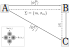
\includegraphics[draft=false, width=\linewidth]{qds/qds_setup}
\caption{\label{fig:qds_setup} Setup of the QDS protocol considered in this chapter. Alice (A) wishes to securely sign a $1$~bit message $m$. Alice distributes quantum coherent states $\ket{\phi_j^{\left(B, C\right)}}$ along insecure quantum distribution channels (solid lines) during the Distribution stage. Bob and Charlie swap eliminated signature elements via their securely encrypted classical channel (dotted lines). During the Messaging stage Alice sends $\Sigma$, containing her message $m$ and her corresponding signature $\sigma_m$ along a classical broadcast channel (dot-dashed line). Inset: QPSK alphabet.}
\end{figure}


Our QDS scheme is split into two stages, Distribution and Messaging, which, by analogy with classical digital signatures, may occur with significant time delay. Quantum states are sent and measured during Distribution. During Messaging Alice will send her message and classical signature, and recipients Bob and Charlie will try to determine its validity.\footnote{Note the intrinsic separation between the Distribution (quantum) and Messaging (classical) stages of the protocol. We will take further advantage of this separation between quantum and classical steps in Chapter~\ref{chapter:aqc}} Our protocol setup is outlined in Figs.~\ref{fig:qds_cartoon},~\ref{fig:qds_setup}. 
\par
\noindent We will now describe in detail the running of the protocol.



\subsubsection{Distribution stage}

\paragraph{Step $1$.}
Alice wishes to send a signed $1$ bit message $m$ to Bob and Charlie. For each possible future $m$, and for each recipient, Alice creates the following classical strings
\begin{equation}
\Phi_m^{\left(B, C\right)} = \left\{ \phi_{j, m}^{\left(B, C\right)}\right\}_{j=1}^{L}
\end{equation}
which are of length $j$. The $\phi_{j}$ are complex phases chosen uniformly at random from the QPSK alphabet. The strings $\Phi_m^{\left(B, C\right)}$ may be interpreted as Alice's \emph{private key}. The signature length $L \in \mathbb{N}$ is chosen to ensure the desired level of security.

\paragraph{Step $2$.} Corresponding to each private key, Alice forms the following quantum states
\begin{equation}\label{eqn:QDS_publickey}
\rho\left[\Phi_m^{\left(B, C\right)}\right] := \otimes_{j=1}^L \; \rho\left[\phi_{j, m}^{\left(B, C\right)}\right]
\end{equation}
with
\begin{equation}
\rho\left[\phi_{j, m}^{\left(B, C\right)}\right] := \ket{\phi_{j, m}^{\left(B, C\right)}} \bra{\phi_{j, m}^{\left(B, C\right)}} \notag
\end{equation}
understood to be the coherent state from QPSK with phase corresponding to the relevant element of Alice's private key.

The states Eq.~\ref{eqn:QDS_publickey} may be interpreted simply as sequences of coherent states, and correspond to Alice's \emph{public key}. An important difference between quantum and classical digital signatures is that here the public key may no longer be freely distributed, copied and stored. We also note that Alice no longer has a single public key for each message (unlike Lamport's scheme \cite{Lamport1979}), and her quantum public key differs both for each possible $m$ and for each recipient (unlike the recent scheme Ref.~\cite{Croal2016}). This is a requirement for security against an eavesdropping forger, Sec.~\ref{sec:qds_security_forgery}.

\paragraph{Step $3$.}
Each recipient $B, C$ performs heterodyne detection on their received coherent states, and receives outcomes $\left( \qout, \pout \right)$ which we will write as $z = \qout + i \pout \in \mathbb{C}$. Crucially, since measurement is performed immediately on receipt of the states no quantum memory is required. The remainder of the protocol is entirely classical.


At the end of the quantum stage of the protocol, recipients Bob and Charlie now possess classical strings, length $L$, containing their phase measurements on Alice's distributed states. They now form \emph{eliminated signatures}, Fig.~\ref{fig:elimsig}. For each $z \in\mathbb{C}$, recipients record the phases $\phi_{j, m}^{\left(B, C\right)}$ which Alice was \emph{least likely} to have sent. At position $j$ this may be understood as computing the four conditional probabilities 
\begin{equation}
p\left(\phi_j \given x_j\right) \qq{for each phase} \phi_j \in \text{QPSK},
\end{equation}
and recording the two $\phi_j$ which yield the smallest of these. This record of $\phi_j$ forms the $j^{\text{th}}$ element of their eliminated signatures. We note that the $\phi_j$ comprising the eliminated signature element will always be adjacent in phase space, and an example of this elimination procedure is displayed in Fig.~\ref{fig:elimsig}. We denote Bob and Charlie's total eliminated signatures at this stage as $X_m^{\left(B, C\right)}$. Each is of length $L$ and they will later be compared to Alice's private key in order to test the validity of the message. We display the possible eliminated signature elements and their requisite heterodyne outcomes in Tab.~\ref{tab:elimsig}.

\begin{figure}[htp]
\captionsetup{width=0.8\linewidth}
\centering
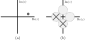
\includegraphics[draft=false, width=\linewidth]{qds/elimsig}
\caption{\label{fig:elimsig} Bob and Charlie each perform heterodyne measurement on their received coherent states, and obtain $\left(\qout, \pout\right)$. We define $z = \qout + i \pout$, which is the dark gray circle in (a). From their $z$, Bob and Charlie then record the two states from QPSK which are least likely to have been sent by Alice, (b). We display the possible eliminated signature elements and their requisite heterodyne outcomes in Tab.~\ref{tab:elimsig}.}
\end{figure}


\begin{table*}
\captionsetup{width=0.8\linewidth}
\centering \ra{1.75}
\begin{tabular*}{\linewidth}{@{\extracolsep{\stretch{1}}} c c c}

\head{Element} & \head{QPSK elements} & \head{Heterodyne outcome} \\ 
\hline 
$e_1$ & $\ket{- \phantom{i}\alpha}, \ket{- i \alpha}$ & $\qout >0, \pout >0$ \\ 

$e_2$ & $\ket{- i \alpha}, \ket{\phantom{-i}\alpha}$ & $\qout < 0, \pout > 0$ \\ 

$e_3$ & $\ket{\phantom{-i}\alpha}, \ket{\phantom{-}i \alpha}$ & $\qout < 0, \pout < 0 $ \\ 

$e_4$ & $\ket{\phantom{-}i \alpha}, \ket{- \phantom{i} \alpha}$ & $\qout > 0, \pout < 0$ \\ 
%\hline
\end{tabular*} 
\caption{\label{tab:elimsig} We denote possible eliminated signature elements as $e_1, e_2, e_3, e_4$, and display their corresponding states from QPSK and their requisite heterodyne measurement outcomes.}
\end{table*}



\paragraph{Step $4$. \emph{Symmetrization:}}
Bob and Charlie now swap a random $L/2$ elements of their $X_m^{\left(B, C\right)}$ over their encrypted classical channel. Signature elements which have been forwarded by a player will no longer be used by him in the protocol. We denote these resulting strings as $Y_m^{\left(B, C\right)}$. By using an encrypted classical channel the positions and values of swapped elements are kept secret from Alice, which will ensure that the information which Bob and Charlie each hold is symmetric from Alice's point of view \cite{Dunjko2014, Wallden2015}. 

In other words, at the end of Step~$3$, having sent the state $\ket{\phi_{j, m}^B}\bra{\phi_{j, m}^B}$ to Bob, Alice knows that Bob holds the corresponding eliminated signature element $X_{j, m}^B$, even though she doesn't know its value. Since Alice knows which state she sent to Bob, she may gain an advantage in trying to guess $X_{j, m}$. At the end of Step~$4$ however, Alice does not know whether it is Bob or Charlie who holds $X_{j, m}^B$. This uncertainty will prove crucial for preventing successful repudiation.

Bob (Charlie) now possesses an eliminated signature $\tilde{X}_m^{\left(B\right)}$ in two halves: one half $Y_m^{\left(B\right)}$ ($Y_m^{\left(C\right)}$) containing those elements received directly from Alice, and one half $Z_m^{\left(B\right)}$ ($Z_m^{\left(C\right)}$) containing elements received during this Symmetrization step from Charlie (Bob).

The key parameters for the Distribution stage are the signature length $L$, which directly measures the quantum resources required for the protocol, and the alphabet parameter $\alpha$, related to the average photon number of the distributed coherent states. Channel parameters such as loss and thermal noise will be discussed later\footnote{In Appendix~\ref{appendix:qds_larger_alphabets} we discuss an extension to the protocol which allows it to run with an $N$PSK alphabet of coherent states, where $N$ is an even integer.}.


\subsubsection{Messaging stage}

Messaging may occur at any time after Distribution.

\paragraph{Step $5$.}
To sign $m$, Alice sends to Bob the classical information $\Sigma = \left(m, \sigma_m\right)$, consisting of the message $m$ which she would like to convey, and her private key $\sigma_m = \left(\Phi_m^B, \Phi_m^C\right)$ consisting of declared phases, which acts as $m$'s signature. 


\paragraph{Step $6$.} Bob rearranges $\sigma_m \rightarrow \tilde{\sigma}_m^B := \left(\tilde{\Phi}_{Y, m}^B, \tilde{\Phi}_{Z, m}^B\right)$ by selecting elements from Alice's declaration which correspond to the two halves of his eliminated signature $\tilde{X}_m^{\left(B\right)}$. The original $\sigma_m$ has length $2 L$, while $\tilde{\sigma}_m^B$ has length $L$.

Bob compares relevant elements of $\tilde{\sigma}_m^B$ to his $\tilde{X}_m^{B}$, choosing which half of $\tilde{X}_m^B$ to compare to based on whether he kept or swapped the eliminated signature element. Bob makes a decision about whether to accept $m$ as genuine based on the number of \emph{mismatches} between Alice's signature and his own eliminated signatures. A mismatch is defined below in Sec.~\ref{sec:qds_mismatches} and in Fig.~\ref{fig:qds_mismatches}.


If Bob measures fewer than $s_B L/2$ mismatches on both of his eliminated signature halves then he accepts Alice's message as genuine, otherwise the protocol aborts. Bob's threshold mismatch rate $s_B$ determines how many mismatches he can observe before a signature fails his check. In general, $s_B$ is a free parameter of the protocol and will be discussed further in Secs.~\ref{sec:qds_mismatches},~\ref{sec:qds_security_repudiation},~\ref{sec:qds_siglength}.

%If Bob measures sufficiently few mismatches on both of his eliminated signature halves
%, i.e. if $\mathcal{M}\left(\tilde{\Phi}_{Y, m}^B, Y_m^B\right) < s_B L/2$ and $\mathcal{M}\left(\tilde{\Phi}_{Z,m}^B, Z_m^B\right) < s_B L/2$ 
%then he accepts Alice's declaration $m$ as genuine, otherwise the protocol aborts. %The threshold $0 \le s_B \le 1$ is related to the security of the protocol and will be discussed later.

\paragraph{Step $7$.} If Bob has accepted $m$, then he forwards $\Sigma$ to Charlie, who similarly checks for mismatches between Alice's signature and his eliminated signature. Charlie accepts the message if %$\mathcal{M}\left(\tilde{\Phi}_{Y, m}^C, Y_m^C\right) < s_C L/2$ and $\mathcal{M}\left(\tilde{\Phi}_{Z, m}^C, Z_m^C\right) < s_C L/2$, with security threshold $0 \le s_c \le 1$ to be discussed later. 
there are fewer than $s_C L/2$  mismatches between $\tilde{\sigma}_m^C$ and $\tilde{X}_m^{\left(C\right)}$. If Charlie also accepts $m$ then the protocol has succeeded, otherwise it aborts.  Charlie's threshold mismatch rate is $s_C$ and will be discussed further in Secs.~\ref{sec:qds_mismatches},~\ref{sec:qds_security_repudiation},~\ref{sec:qds_siglength}.

The key parameters for the Messaging stage are $s_B, s_C$ which may be freely chosen by Bob and Charlie in order to optimize security. We observe in Sec.~\ref{sec:qds_security_repudiation} that the choice $s_B \le s_C$ will ensure security against Alice's repudiation attack.

%\clearpage
\subsection{Counting mismatches}\label{sec:qds_mismatches}

\begin{figure}[htp]
\captionsetup{width=0.8\linewidth}
\centering
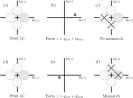
\includegraphics[draft=false, width=\linewidth]{qds/mismatch1}
\caption{\label{fig:qds_mismatches} A mismatch occurs when an honest party eliminates the state which Alice claims to have sent. (a, d) Alice sends coherent state $\ket{\alpha}$. (b, e) Bob (Charlie) heterodynes and receives $\left(\qout, \pout\right)$. We define $z = \qout + i \pout$. Even when all players are honest there is some probability of measuring $\qout < 0$, Sec.~\ref{sec:qds_modelling_perr}. (c) The eliminated signature element consists of $\ket{- \alpha}, \ket{- i \alpha}$ so there is no mismatch. (f) The eliminated signature element consists of $\ket{\alpha}, \ket{i \alpha}$ and so there is a mismatch.}
\end{figure}


The key test of validity which our protocol employs is a check on the number of mismatches between Bob or Charlie's eliminated signatures $\tilde{X}^{\left(B, C\right)}_m$ and Alice's declaration $\sigma_m$. A mismatch occurs if the state which Alice claims to have sent has been eliminated, Fig.~\ref{fig:qds_mismatches}. 

To be concrete, a mismatch occurs at position $j$ if
\begin{equation}
\phi_{j, m}^{B \left(C\right)} \in Y_{j, m}^{B \left(C\right)} \qq{or} \phi_{j, m}^{C \left(B\right)} \in Z_{j, m}^{B \left(C\right)}, 
\end{equation}
and we let
\begin{equation}
\mathcal{M}\left(F, G\right)
\end{equation}
denote the probability of mismatch between an arbitrary eliminated signature $G$, and an arbitrary list of phases $F$. Both $F$ and $G$ should be of the same length.

%denote the probability of mismatch between arbitrary declared signature $F$ and arbitrary eliminated signature $G$.\MT{I think this should be more concrete}



\section{Security against repudiation}\label{sec:qds_security_repudiation}
\iffalse
In other words at the end of Step~$3$, having sent the state $\ket{\phi_{j, m}^B}\bra{\phi_{j, m}^B}$ to Bob, Alice knows that Bob holds the corresponding eliminated signature element $X_{j, m}^B$. Since Alice knows which state she sent to Bob, she may be able to guess Bob's eliminated signature element with some probability. 

 At the end of Step~$4$ however, Alice does not know whether it is Bob or Charlie who holds $X_{j, m}^B$. This uncertainty will prove crucial for preventing her from successfully repudiating (Requirement~$3$). Bob (and Charlie) now possesses an eliminated signature $\tilde{X}_m^{\left(B\right)}$ in two halves: one half ($Y_m^{\left(B\right)}$) containing those elements received directly from Alice, and one half ($Z_m^{\left(B\right)}$)containing elements received during this Symmetrization step from Charlie.
 \fi


We now turn to consider the security of the QDS protocol desribed in Sec.~\ref{sec:qds_protocol}. %Recall that of the five requirements for a digital signatures protocol, requirements $3$ and $4$ are equivalent in a $3$~party setting. 
In what follows we will prove that our protocol is:
\begin{enumerate}
\item Sec.~\ref{sec:qds_security_repudiation}: secure against a repudiation attack (List~\ref{list:qds_requirements}~requirement $3$, Fig.~\ref{fig:attacks_repudiation}), 
\item Sec.~\ref{sec:qds_security_robustness}: robust (List~\ref{list:qds_requirements} ~requirement $5$, Fig.~\ref{fig:attacks_robustness}),
\item Sec.~\ref{sec:qds_security_forgery} secure against a forgery attack (List~\ref{list:qds_requirements}~requirement $1$, Fig.~\ref{fig:attacks_forgery})
\end{enumerate}

Our proof will proceed by demonstrating that an attempted repudiation or forgery will induce a large mismatch rate, while a small mismatch rate is obtained when no attack is attempted. Thus, by appropriate choice of security parameters $s_B, s_C$ and signature length $L$, the probability of a \emph{successful} attack of any type may be made arbitrarily small. 

We assume that in our $3$~party setting at most one of the players $A, B, C$ may behave dishonestly. For simplicity of notation we give a dishonest player the power to eavesdrop on the distribution of quantum states, and so the label ``Eve'' is not required. An internal eavesdropper is at least as powerful as an external Eve. If two or more players are dishonest then we assume that they will collaborate, which allows them to trivially break the protocol, and so this scenario is not discussed. We note that a collaboration of multiple dishonest players must be considered for an $n>3$~party QDS protocol, as discussed in Ref.~\cite{Arrazola2016}.

To succeed in a repudiation attack, a dishonest Alice aims to convince Bob that message $m$ is genuine, while Charlie that $m$ is fake, Fig.~\ref{fig:attacks_repudiation}. Security against repudiation is guaranteed by the symmetrization procedure (Step $4$ of the protocol) which ensures that Alice does not know which recipient holds the eliminated signature element corresponding to a particular distributed state. Proof of security against repudiation follows along similar lines to Refs.~\cite{Dunjko2014, Wallden2015, Donaldson2016, Croal2016, Thornton2019}.

At the end of Step~$3$, having sent the state $\ket{\phi_{j, m}^B}\bra{\phi_{j, m}^B}$ to Bob, Alice knows that Bob holds the corresponding eliminated signature element $X_{j, m}^B$, and she may be able to guess it with high probability. In any case, knowing which recipient holds the $X_{j, m}^{\left(B, C\right)}$ gives Alice additional power to repudiate, even if she does not know what the individiual eliminated signature elements are\footnote{Alice could, for example, perform an optimal strategy in order to guess the $X_{j, m}^{\left(B, C\right)}$. Then she may declare $\sigma_m$ using guesses on Bob's elements to reduce her mismatch rate with respect to Bob, while declaring the opposite of her guesses on Charlie's elements to increase her mismatch rate with respect to Charlie.}.

At the end of Step~$4$, however, Alice does not know whether it is Bob or Charlie who holds an element $X_{j, m}^B$. This uncertainty will prove crucial for preventing her from successfully repudiating. Recall that Bob  (Charlie) possesses an eliminated signature $\tilde{X}_m^{\left(B\right)}$ in two halves: one half ($Y_m^{\left(B\right)}$) containing those elements received directly from Alice, and one half ($Z_m^{\left(B\right)}$) containing elements received during this symmetrization step from Charlie (Bob).

We assume that Alice is completely free to manipulate her declared $\sigma_m = \left(\Phi_m^B, \Phi_m^C\right)$. We also assume that she may freely manipulate the number of mismatches %$\mathcal{M}\left(\Phi_m^{B, C}, X_m^{\left(B, C\right)}\right)$ 
between her declared signature and the eliminated signatures $X_m^{\left(B, C\right)}$ which Bob or Charlie held before symmetrization. We denote these observed mismatch rates as $p_B$ and $p_C$, respectively: 

\begin{align}
p_B &= \mathcal{M}\left(\Phi_m^B, X_m^B\right), \notag \\
p_C &= \mathcal{M}\left(\Phi_m^C, X_m^C\right).
\end{align}
Alice may even choose them to be zero

%After Symmetrization, Bob and Charlie each possess an eliminated signature in two halves, each of length $L/2$, consisting either of elements which they received directly from Alice, or of elements which they received during this step. 

Alice succeeds in her repudiation attack if Bob accepts both of his halves as genuine, while Charlie rejects at least one of his halves as fake. Let $E_A, E_B$ denote the events that Bob accepts on the first or second half of his eliminated signature, respectively, and let $E_C, E_C$ denote the events that Charlie rejects on the first or second half of his eliminated signature, respectively. Then a successful repudiation attack occurs when

\begin{equation}
\left(E_A \qq{and} E_B \right) \qq{and} \left( E_C \qq{or} E_D\right) \notag
\end{equation}
where the events are defined as
\begin{align}\label{eqn:repudiation_events}
&E_A \qq{when} \mathcal{M}\left(\tilde{\Phi}_{Y, m}^B, Y_m^B\right) < s_B L/2,  \notag \\
%
&E_B \qq{when} \mathcal{M}\left(\tilde{\Phi}_{Z, m}^B, Z_m ^B\right) < s_B L/2, \notag \\
%
&E_C \qq{when} \mathcal{M}\left(\tilde{\Phi}_{Y, m}^C, Y_m^C\right) \ge s_C L/2, \notag \\
%
&E_D \qq{when} \mathcal{M}\left(\tilde{\Phi}_{Z, m}^C, Z_m^C\right) \ge s_C L/2 .
\end{align}
The $\tilde{\Phi}$ denotes the rearranged form of Alice's declared phases $\Phi$ in order to compare corresponding elements, symbol $Y$ denotes that an element was received directly from Alice and symbol $Z$ denotes that it was received during symmetrization. Function $\mathcal{M}$ measures the mismatch probability between two strings, and is defined above in Sec.~\ref{sec:qds_mismatches}.

Thus, the probability $\varepsilon_{\text{repudiation}}$ of a successful repudiation attack is given by

\begin{equation}
\varepsilon_{\text{repudiation}} = \text{P}\left[\left(E_A \cap E_B\right) \cap \left(E_C \cup E_D\right)\right].
\end{equation}
To proceed, we require the following two probability inequalities for arbitrary events $x, y$:

\begin{align}
\label{eqn:prob_inequality_1}
\text{P}\left(x \cap y\right) &\le \text{min}\left\{\text{P}\left(x\right), \text{P}\left(y\right)\right\}, \\
\label{eqn:prob_inequality_2}
\text{P}\left(x \cup y\right) &\le \text{P}\left(x\right) + \text{P}\left(y\right).
\end{align}
\noindent We may now use the probability inequality Eq.~\ref{eqn:prob_inequality_1} and observe that 

\begin{equation}
\varepsilon_{\text{repudation}} \le \text{min}\left\{\text{P}\left(E_A \cap E_B\right), \text{P}\left(E_C \cup E_D\right)\right\}. \notag
\end{equation}

\noindent Again using Eqs.~\ref{eqn:prob_inequality_1},~\ref{eqn:prob_inequality_2}, we arrive at

\begin{equation}\label{eqn:rep_prob_working}
\varepsilon_{\text{repudiation}} \le \text{min}\left\{
\text{min}\left\{\text{P}\left(E_A\right), \text{P}\left(E_B\right) \right\}, \text{P}\left(E_C\right) + \text{P}\left(E_D\right)\right\},
\end{equation}
which provides an upper bound for the probability of successful repudiation attack in terms of the individual probabilities for distinct events. We now wish to demonstrate that the probability for each event may be made arbitrarily small by suitable choice of $L$, and thus $\varepsilon_{\text{repudiation}}$ may also be made arbitrarily small.


We rely on Hoeffding's inequalities Eqs.~\ref{eqn:hoeffding1},~\ref{eqn:hoeffding2} which we use to bound each probability appearing in Eq.~\ref{eqn:rep_prob_working}. Let $\mathcal{F}$ be a string of declared phases, and $\mathcal{G}$ be an eliminated signature. Strings $\mathcal{F}$ and $\mathcal{G}$ each have length $n$. We define a string $\mathcal{E}$ such that

\begin{equation*}\label{eqn:error_qds}
\mathcal{E}_j = 
\begin{cases}
1 & \text{if a mismatch occurs between $\mathcal{F}_j$ and $\mathcal{G}_j$} \\
0 & \text{otherwise}
\end{cases}
\end{equation*}
which measures whether a mismatch has occurred between the $j^\text{th}$ elements of $\mathcal{F}$ and $\mathcal{G}$, Fig.~\ref{fig:qds_mismatches}, Sec.~\ref{sec:qds_mismatches}.


The mismatch rate $\mathcal{M}\left(\mathcal{F}, \mathcal{G}\right)$ is equivalent to the observed (empirical) mean $\bar{\mathcal{E}}$, while its expectation $\mathbb{E}\left(\bar{\mathcal{E}}\right)$ is equal to the arithmetic mean
\begin{equation}
\mathbb{E}\left(\bar{\mathcal{E}}\right) = \frac{1}{n} \sum_{j=1}^n \mathcal{E}_j. \notag
\end{equation}

\noindent We wish to bound the probability that there are fewer than $s$ observed mismatches,
\begin{equation}
\text{P}\left(\mathcal{M}\left(\mathcal{F}, \mathcal{G}\right) \le s\right) = \text{P}\left( \mathbb{E}\left(\bar{\mathcal{E}}\right) - \bar{\mathcal{E}} \ge \mathbb{E}\left(\bar{\mathcal{E}}\right) - s\right).
\end{equation}
By applying Hoeffding inequality Eq.~\ref{eqn:hoeffding1},

\begin{equation}\label{eqn:qds_hoeffding1}
\text{P}\left(\mathcal{M}\left(\mathcal{F}, \mathcal{G}\right) \le s \right) \le \text{exp}\left(- 2 \left[\mathbb{E}\left(\bar{\mathcal{E}}\right) - s\right]^2 n \right)
\end{equation}
provided that $\mathbb{E}\left(\bar{\mathcal{E}}\right) - s \ge 0$. This Eq.~\ref{eqn:qds_hoeffding1} gives an upper bound for the probability that there are fewer than $s$ mismatches observed when the average probability for mismatch is $\mathbb{E}\left(\bar{\mathcal{E}}\right)$.

Similarly, we derive
\begin{equation}\label{eqn:qds_hoeffding2}
\text{P}\left(s \le \bar{\mathcal{E}}\right) \le \text{exp}\left( - 2 \left[s - \mathbb{E}\left(\bar{\mathcal{E}}\right)\right]^2 n\right)
\end{equation}
by applying Eq.~\ref{eqn:hoeffding2}, provided that $s - \mathbb{E}\left(\bar{\mathcal{E}}\right) \ge 0$. This Eq.~\ref{eqn:qds_hoeffding2} gives an upper bound for the probability that there are more than $s$ mismatches observed when the average probability for mismatch is $\mathbb{E}\left(\bar{\mathcal{E}}\right)$. 


Using Eqs.~\ref{eqn:qds_hoeffding1},~\ref{eqn:qds_hoeffding2} we may now bound the probabilities for events of Eq.~\ref{eqn:repudiation_events}:

\begin{align}\label{eqn:qds_repudiation_events_probs}
\text{P}\left(E_A\right) \le \text{exp}\left( -\left[p_B - s_B\right]^2 L \right) \qq{provided that} p_B > s_B, \notag \\
\text{P}\left(E_B\right) \le \text{exp}\left( -\left[p_C - s_B\right]^2 L \right) \qq{provided that} p_C > s_B, \notag \\
\text{P}\left(E_C\right) \le \text{exp}\left( -\left[s_C - p_C\right]^2 L \right) \qq{provided that} p_C < s_C, \notag \\
\text{P}\left(E_D\right) \le \text{exp}\left( -\left[s_C - p_B\right]^2 L \right) \qq{provided that} p_B < s_C,
\end{align}

\noindent where in the first two inequalities we have applied Eq.~\ref{eqn:qds_hoeffding1} and in the second two inequalities we have applied Eq.~\ref{eqn:qds_hoeffding2}. 

Alice has the power to choose any $0 \le p_B, p_C \le 1$. Let us consider some cases.

\paragraph{Case 1:} Assume that $p_B \ge s_B$. Then, by the first inequality of Eq.~\ref{eqn:qds_repudiation_events_probs}, the probability Eq.~\ref{eqn:rep_prob_working} must decay exponentially %must it? Could we decay faster? 
and so we are secure against repudiation. An analogous argument holds for the choice $p_C \ge s_B$ using the second inequality of Eq.~\ref{eqn:qds_repudiation_events_probs}.

\paragraph{Case 2:} Assume that $p_B < s_B$ and $p_C < s_B$. It follows that if we choose $s_B \le s_C$, then we force $p_B < s_C$ and $p_C < s_C$, and so Eq.~\ref{eqn:rep_prob_working} decays exponentially via the third and fourth inequalities of Eq.~\ref{eqn:qds_repudiation_events_probs}. Intuitively, we have demonstrated that even though Alice has full control over $p_B, p_C$ she cannot engineer a situation in which Bob measures fewer than $s_B$ mismatches while Charlie measures more than $s_C$. This relies on the choice $s_B \le s_C$ to ensure that $\varepsilon_{\text{repudiation}}$ decays exponentially in $L$.


Let us substitute Eq.~\ref{eqn:qds_repudiation_events_probs} into Eq.~\ref{eqn:rep_prob_working} and simplify. Clearly, increasing $p_B$ or $p_C$ will cause both of the exponentials in the first term to decrease. Because of the inner minimum, we will only care about $\text{max}\left\{p_B, p_C\right\}$, and so we define $p := \text{max}\left\{p_B, p_C\right\}$ and write

\begin{equation}
\text{min}\left\{\text{exp}\left(- \left[p_B - s_B\right]^2L\right), \; \text{exp}\left(- \left[p_C - s_B\right]^2L\right)\right\} = \text{exp}\left(-\left[p - s_B\right]^2L\right). \notag
\end{equation}
In the case $p_B, p_C \le s_C$ we may increase the second term of Eq.~\ref{eqn:rep_prob_working}:

\begin{equation}
\text{exp}\left(- \left[s_C - p_C\right]^2 L \right) + \text{exp}\left(- \left[s_C - p_B\right]^2 L \right) \le 2 \exp\left( - \left[s_C - p\right]^2 L\right).
\end{equation}
This leads to

\begin{equation}
\varepsilon_{\text{repudiation}} \le \text{min}\left\{ 2 \; \text{exp}\left( - \left[p - s_B\right]^2 L \right), 2 \; \text{exp}\left( - \left[s_C - p\right]^2 L \right) \right\}.
\end{equation}
Since the minimum over two distinct Gaussians is maximized when the Gaussians have equal arguments, the probability $\varepsilon_{\text{repudiation}}$ is maximized when 
\begin{equation}
p = \frac{s_B + s_C}{2}.
\end{equation}

\noindent Finally, we reach
\begin{equation}\label{eqn:erep}
\varepsilon_{\text{repudiation}} \le 2 \text{exp}\left( - \frac{\left[s_C - s_B\right]^2}{4} L\right)
\end{equation}
as our useful bound for the probability that Alice succeeds in her repudiation attack. Since Eq.~\ref{eqn:erep} is exponentially decaying, the probability that she succeeds may be made arbitrarily small by choice of $L$. Our protocol can therefore be secured against a repudiation attack by a sufficiently large choice of $L$, provided that we choose $s_B \le s_C$.




\section{Robustness}\label{sec:qds_security_robustness}
The QDS protocol must be robust (List~\ref{list:qds_requirements} requirement~$5$, Fig.~\ref{fig:attacks_robustness}) and allow the message $m$ to be accepted provided that all parties behave honestly and there is no attack present. This is a requirement for useful QDS, since a protocol which aborts for every message will certainly abort in the presence of an attack and thus is trivially secure. In this Section we will find an upper bound to the probability that the protocol fails even when everyone behaves honestly.

The protocol fails in the absence of attack if either Bob or Charlie rejects a message which Alice did in fact send, i.e. if Bob or Charlie detect too many mismatches on Alice's declaration $\sigma_m$. Since in Sec.~\ref{sec:qds_security_repudiation} we derived that $s_B \le s_C$, it will always be more likely that Bob rejects than Charlie. We will seek to bound the probability that Bob measures more than $s_B L/2$ mismatches on either of his signature halves. This will also provide an upper bound for the probability that Charlie rejects with no attack.

We define an \emph{honest mismatch} to have occured if there is a mismatch between Alice's declaration and either of Bob's (or Charlie's) eliminated signature halves in an honest scenario. Let $\perr$ be the probability of honest mismatch. Because of the non-orthogonality of coherent states even in an ideal setting we have $\perr > 0$. This is in contrast to protocols such as Refs.~\cite{Donaldson2016, Collins2014} which could attain an ideal $\perr = 0$. We model $\perr$ in the next Section~\ref{sec:qds_modelling_perr}, and there demonstrate that it is nonzero.

Using probability inequality Eq.~\ref{eqn:prob_inequality_2}, the probability that Bob rejects either of his halves is given by

\begin{equation}
\varepsilon_{\text{Bob rejects}} \le 2 \text{P}\left(E_A\right)
\end{equation}
where $E_A$ is the event that Bob measures more than $s_B L/2$ mismatches on either of his halves. We have implicitly assumed that $\perr$ is identical for states originally sent to Bob and those originally sent to Charlie, but this is easy to relax if desired.

Using Hoeffding inequality Eq.~\ref{eqn:qds_hoeffding2} in an identical manner to the derivation of Eq.~\ref{eqn:qds_repudiation_events_probs}, Sec.~\ref{sec:qds_security_repudiation}, we see that
\begin{equation}\label{eqn:ehonabort}
\varepsilon_{\text{honest abort}} = \varepsilon_{\text{Bob rejects}} \le 2 \exp\left( - \left[s_B -\perr\right]^2 L\right)
\end{equation}
provided that $s_B - \perr \ge 0$. Equation~\ref{eqn:ehonabort} is our useful bound for the probability that the protocol fails the robustness requirement. Since it is exponentially decaying, the probability that this happens can be made arbitrarily small, and so our protocol is robust.

\subsection{Modelling $p_{\text{err}}$}\label{sec:qds_modelling_perr}

The probability $\perr$ corresponds to the probability that a heterodyne measurement outcome $\left(\qout, \pout\right)$ has $\qout < 0$ when Alice distributed the coherent state $\ket{\alpha}$, Fig.~\ref{fig:perr}. In the absence of thermal noise the channel simply acts as a beamsplitter with vacuum at the unused input port, and so

\begin{equation}
\ket{\alpha}_A \rightarrow \ket{\sqrt{T}\alpha}_{\left(B, C\right)}
\end{equation}


\noindent when the channel has transmission $T$ (see Appendices~\ref{appendix:noisy_perr},~\ref{appendix:crypto_numerical_methods}). A heterodyne measurement on the output state yields $\left(\qout, \pout\right)$ which we write as $z = \qout + i \pout$. We receive $z$ with probability
\begin{align}
\text{P}\left(z\right) = \frac{1}{\pi}\text{exp}\left( - \left| z - \sqrt{T}\alpha \right|^2 \right)
\end{align}
where ket vector $|z\rangle$ denotes the coherent state centred on $z$ (c.f. Appendix~\ref{appendix:noisy_perr}). Then,

\begin{align}
\perr &= \text{P}\left(\text{Re}\left(z\right)<0\right) = \int\limits_{\text{Re}\left(z\right)<0}\Diff2 z \, \text{P}\left(z\right) \notag \\
&= \int\limits_{-\infty}^{\infty} \mathrm{d} y \, \text{exp}\left(-y^2\right) \int\limits_{-\infty}^{0} \mathrm{d} x \, \text{exp}\left(-\left[x - \sqrt{\frac{T}{2}}\alpha_x\right]^2\right),
\end{align}
where $x = \text{Re}\left(z\right)=\qout, y = \text{Im}\left(z\right)=\pout$ and $\alpha_x = \text{Re}\left(\alpha\right)$. 

Integrating, we arrive at

\begin{equation}\label{eqn:perr}
\perr = \frac{1}{2}\text{erfc}\left(\sqrt{\frac{T}{2}}\alpha\right)
\end{equation}

\noindent which models the probability of honest mismatch over a lossy channel with transmission $T$. Probability $\perr$ is motivated in Fig.~\ref{fig:perr} which elucidates the above discussion, and explains why $\perr \ne 0$. An equivalent analysis when the channel contains thermal noise is discussed in Appendix~\ref{appendix:noisy_perr}.

\begin{figure}[htp]
\captionsetup{width=0.8\linewidth}
\centering
\includegraphics[draft=false, width=0.8\linewidth]{qds/perrnonzero}
\caption{\label{fig:perr} Histogram of possible heterodyne outcomes. A coherent state $\ket{\alpha}$ with $\alpha>0$ has nonzero probability to give the measurement outcome $\qout < 0$. In other words, $\perr > 0$ always, and $\perr \rightarrow 0$ only as $\alpha \rightarrow \infty$. The blue region corresponds to measurement outcomes which will not give a mismatch, while the pink region corresponds to measurement outcomes which will yield a mismatch. This histogram is equivalent to the Hussimi $Q$ function \cite{Leonhardt2010} of the received coherent state, and is thus also Gaussian.}
\end{figure}


\section{Security against forgery}\label{sec:qds_security_forgery}
We now turn to consider security against forgery, List.~\ref{list:qds_requirements}~requirement $1$, Fig.~\ref{fig:attacks_forgery}. In a forging attack, a dishonest player (or a fourth party, Eve) will declare some fake $m^\prime$ with the aim that it should be accepted by honest players as being genuine and having originated with Alice. % In this attack we consider two possibilities, either that an honest Alice's $\Sigma$ has been intercepted and altered (interferance in Step $5$); or that honest Alice has completed distribution of quantum states, Step $3$, but has not yet sent $\Sigma$. As should be clear from the following discussion 
We will not consider the possibility that a dishonest player is impersonating Alice from the beginning of the protocol (see Sec.~\ref{sec:qds_goals} for brief discussion). The fake message $m^\prime$ will have an appended signature $\tau_{m^\prime}$ consisting of declared coherent state phases. Message $m^\prime$ will be accepted if $\tau_{m^\prime}$ has sufficiently few mismatches with respect to an honest player's eliminated signature. 

%Since Bob already knows $L/2$ of Charlie's elements, precisely those $Z_m^C$ which originated with Bob,

Since Bob and Charlie already know $L/2$ of each other's eliminated signature elements -- those which were forwarded during the symmetrization step of the protocol -- a dishonest player who is internal to the signature scheme will always have an advantage over an external Eve. Additionally, since $s_B < s_C$, Charlie is more likely than Bob to accept a forged message $m^\prime$ and fake signature $\tau_{m^\prime}$, and so the most dangerous forger will be a dishonest Bob. We thus proceed with the mantra ``Bob is Eve,'' and take Bob as our dishonest forging party. Since this is a worst-case scenario, our following analysis will implicitly also guard against the possiblity that Charlie or Eve are the forger.

Security against a forging attack arises because the sequence of states which Alice sends to Bob is different from the sequence which she sends to Charlie. This is in stark contrast to the recent work Ref.~\cite{Croal2016} and earlier works Refs.~\cite{Collins2014, Donaldson2016, Dunjko2014, Gottesman2001}. Since Bob already knows the $L/2$ elements $Z_{m}^C$ which Charlie received from Bob during Symmetrization, Step $4$, Bob is able to cause arbitrarily few mismatches on that half of Charlie's signature. Bob's goal then is to declare a string $\tilde{\Phi}^C_{Y, m^\prime}$, length $L/2$ such that 
\begin{equation}\label{eqn:forging_condition}
\mathcal{M}\left(\tilde{\Phi}^C_{Y, m^\prime}, Y_{m^\prime}^C\right) \le s_C \frac{L}{2},
\end{equation}
which will be accepted by Charlie.

Bob's only strategy to gain information about the $Y_{m^\prime}^C$ is to eavesdrop on the distribution of states from Alice to Charlie during Steps~$2$ and $3$ of the protocol, and Bob's eavesdropping strategies will be fully considered in Sec.~\ref{sec:qds_attack_analysis} below.

Defining $\text{p}_e$ as the probability that Bob will induce a mismatch on an individual given signature element, the probability $\varepsilon_{\text{forgery}}$ that Bob succeeds in his forging attack is
\begin{equation}\label{eqn:eforg}
\varepsilon_{\text{forgery}} \le 2 \text{exp}\left( - \left[\text{p}_e - s_C\right]^2 L\right), 
\end{equation}
provided that $\pe - s_C \ge 0$. Equation~\ref{eqn:eforg} is derived using Eq.~\ref{eqn:qds_hoeffding1} similarly to Eqs.~\ref{eqn:erep},~\ref{eqn:ehonabort} in Secs.~\ref{sec:qds_security_repudiation},~\ref{sec:qds_security_robustness} by calculating the probability that Charlie accepts a message with more than $\pe$ mismatches.

Charlie's threshold $s_C$ may be freely chosen, and by combining it with conditions required for derivation of Eqs.~\ref{eqn:erep},~\ref{eqn:ehonabort} we deduce the requirement
\begin{equation}\label{eqn:qds_security_condition}
\perr \le s_B \le s_C \le \pe,
\end{equation}
where threshold parameters $s_B, s_C$ may be freely chosen to optimize security. 

Equation~\ref{eqn:qds_security_condition} encodes the intuitive condition that the QDS protocol is secure provided that $\pe > \perr$; or, in other words, that a dishonest forger will cause more mismatches than an honest player. The protocol security analysis thus relies on finding channel parameters, signature lengths and QPSK amplitudes for which a forger is guaranteed to make more errors than the honest error rate $\perr$, and thus for which a forging attack will be detectable. In Sec.~\ref{sec:qds_bounding_pe} we demonstrate how $\pe$ relates to the quantum system held by Bob at the end of the protocol's Distribution stage, while in Sec.~\ref{sec:qds_attack_analysis} we analyse several types of eavesdropping attack which Bob may attempt, and we perform explicit calculations of $\pe$ under different channel conditions.

%\MT{Make a statement comparing this $\pe \ge \perr$ condition to QKD, where an eavesdropper can hide an attack below channel noise.}

\section{Bounding $\pe$}\label{sec:qds_bounding_pe}
To complete the security analysis of our protocol we must find a lower bound for $\pe$, the rate at which a forging Bob will induce a mismatch with respect to Charlie's signature. Our protocol may be secured by choice of $L$ provided that $\pe > \perr$ and an honest Charlie outperforms dishonest Bob. The key contribution of this section will be a lower bound for $\pe$ which may be calculated once Bob's quantum system at the end of the Distribution stage of the protocol is known.


Bob will declare a string $\tilde{\Phi}_{Y, m^\prime}^C$, length $L/2$, aimed to cause sufficiently few mismatches with respect to Charlie. For convenience we will abbreviate Bob's declared string as $\tilde{\Phi}_{\text{Bob}}$. %Our security analysis must fully take into account the ambiguity in Bob's declarations. This ambiguity stems from the following, and is illustrated in Fig.~\ref{fig:ambiguity}. 
Our analysis differs from QKD analysis in that Bob's mismatch probability is \emph{not equivalent} to the probability that he misidentifies an element of Chalie's eliminated signature. Because Charlie eliminates two states from QPSK, Fig.~\ref{fig:elimsig}, there are two remaining states from the QPSK alphabet which Bob can declare without introducing a mismatch. Each of the remining states is shared with another possible eliminated signature element, and so it is entirely possible for Bob to misidentify Charlie's eliminated signature and yet still not introduce a mismatch.

This forces us to work directly in terms of mismatch probability $\pe$, which we do via our error variable $\mathcal{E}$, Eq.~\ref{eqn:error_qds}, the $j^{\text{th}}$ element of which is $1$ if Bob induces a mismatch there, and $0$ if there is no mismatch. We will continue to work in terms of the QPSK alphabet, though in Appendix~\ref{appendix:qds_larger_alphabets} we demonstrate how the proof may be generalized to an $N$PSK alphabet.

To proceed, recall that $Y_{m^\prime}^C$ is the half of Charlie's eliminated signature based on states he received directly from Alice. This is the half which Bob will attack. We define $Y_j$ to be its $j^{\text{th}}$ element, and write $Y_j = \left\{ y_1^j, y_2^j\right\}$ for phases $y_1^j, y_2^j$ in the QPSK alphabet. The $y_{1,2}^j$ denote the states which Charlie has eliminated. Note that $y_{1,2}^j$ must be adjacent to each other in phase-space, that is, if $y_1^j = \alpha$ then $y_2^j$ must be either $i \alpha$ or $- i \alpha$. The string $\tilde{\Phi}_{\text{Bob}} = \left\{\phi_j\right\}_{j=1}^{L/2}$ is Bob's declaration, which is the result of an unspecified but optimal POVM and classical strategy.

A mismatch occurs when $\phi_j = y_1^j$ or $\phi_j = y_2^j$. Bob's average mismatch rate $\pe$ may be equivalently written in terms of $\mathcal{E}$
\begin{equation}
\pe = \text{P}\left(\mathcal{E}_j = 1\right). \notag
\end{equation}
Because $\mathcal{E}_j$ can take one of two values, the Shannon entropy $\text{H}\left(\mathcal{E}_j\right)$ is equivalent to the binary entropy $\text{h}\left(\pe\right)$, which is defined in Eq.~\ref{eqn:intro_binary_entropy}. %define this equation in introduction chapter.

Now, consider the conditional entropy
\begin{equation}\label{eqn:qds_starting_point}
\text{H}\left(\mathcal{E}_j, y_1^j, y_2^j \given \phi_j\right)
\end{equation}
which is related to the uncertainty about whether a mismatch has occurred under Bob's declaration $\phi_j$. Using the chain rule for conditional entropies, Eq.~\ref{eqn:intro_chain_rule}, we may write
\begin{equation}\label{eqn:qds_pe_deriv_1}
\text{H}\left( \mathcal{E}_j, y_1^j, y_2^j \given \phi_j \right) = 
\text{H}\left( \mathcal{E}_j \given y_1^j, y_2^j, \phi_j\right) + 
\text{H}\left( y_1^j, y_2^j \given \phi_j\right).
\end{equation}
Since an element $\mathcal{E}_j$ is uniquely determined once $\phi_j, y_1^j, y_2^j$ are known, we may immediately deduce
\begin{equation}
\text{H}\left( \mathcal{E}_j \given y_1^j, y_2^j, \phi_j\right) = 0. \notag
\end{equation}

\noindent Using chain rule Eq.~\ref{eqn:intro_chain_rule} once again on the left hand side of Eq.~\ref{eqn:qds_pe_deriv_1}, but this time expanding over variable $y_1^j, y_2^j$, we get:
\begin{align}\label{eqn:qds_pe_deriv_2}
\text{H}\left( \mathcal{E}_j, y_1^j, y_2^j \given \phi_j \right) &=
\text{H}\left(y_1^j, y_2^j \given \mathcal{E}_j, \phi_j\right) + \text{H}\left(\mathcal{E}_j \given \phi_j\right) \notag \\
&\le \text{H}\left(y_1^j, y_2^j \given \mathcal{E}_j, \phi_j\right) + \text{H}\left(\mathcal{E}_j\right) \notag \\
&= \text{H}\left(y_1^j, y_2^j \given \mathcal{E}_j, \phi_j\right) + \text{h}\left(\pe\right)
\end{align}
where the inequality follows because conditioning cannot increase entropy.

Combining Eqs.~\ref{eqn:qds_pe_deriv_1} and \ref{eqn:qds_pe_deriv_2},

\begin{align}\label{eqn:qds_pe_deriv_3}
\text{H}\left(y_1^j, y_2^j \given \phi_j\right) &\le \text{H}\left(y_1^j, y_2^j \given \mathcal{E}_j, \phi_j\right) + \text{h}\left(\pe\right) \notag \\
&= \text{P}\left(\mathcal{E}_j=0\right) \text{H}\left(y_1^j, y_2^j \given \mathcal{E}_j=0, \phi_j\right) \notag \\
&+ \text{P}\left(\mathcal{E}_j=1\right) \text{H}\left(y_1^j, y_2^j \given \mathcal{E}_j=1, \phi_j\right) + \text{h}\left(\pe\right)
\end{align}
with
\begin{equation}
\text{P}\left(\mathcal{E}_j=0\right) = 1 - \pe \qq{and} \text{P}\left(\mathcal{E}_j=1\right) = \pe.
\end{equation}

\noindent Now, because there are two eliminated signature elements consistent with a given $\mathcal{E}_j=0$ and $\phi_j$, and since we are free to permute and relabel $y_1^j \leftrightarrow y_2^j$, we have four choices for the variable $y_1^j, y_2^j$ once $\mathcal{E}_j$ and $\phi_j$ are chosen\footnote{And eight choices \emph{a priori}.}. Thus,
\begin{equation}
\text{H}\left(y_1^j, y_2^j \given \mathcal{E}_j=0, \phi_j\right) \le \log_2 4 = 2.
\end{equation}

\noindent Additionally, since Charlie eliminates precisely half of the alphabet to form his eliminated signature, we see that
\begin{equation}
\text{H}\left(y_1^j, y_2^j \given \mathcal{E}_j=0, \phi_j\right) = \text{H}\left(y_1^j, y_2^j \given \mathcal{E}_j=1, \phi_j\right),
\end{equation}
and so Eq.~\ref{eqn:qds_pe_deriv_3} becomes
\begin{equation}\label{eqn:qds_pe_deriv_4}
\text{H}\left(y_1^j, y_2^j \given \phi_j\right) \le 2 + \text{h}\left(\pe\right).
\end{equation}

\noindent Let us expand the left hand side of Eq.~\ref{eqn:qds_pe_deriv_4} using the definition of mutual information, Eq.~\ref{eqn:intro_mutual_information}:
\begin{equation}\label{eqn:qds_pe_deriv_5}
\text{H}\left(y_1^j, y_2^j \given \phi_j\right) = \text{H}\left(y_1^j, y_2^j\right) - \text{I}\left(y_1^j, y_2^j : \phi_j\right).
\end{equation}

\noindent There are four possible eliminated signature elements, therefore eight possible choices for $y_1^j, y_2^j$ including relabeling $y_1^j \leftrightarrow y_2^j$, and so 
\begin{equation}
\text{H}\left(y_1^j, y_2^j\right) = \log_2 8 = 3.
\end{equation}

\noindent We lower bound Eq.~\ref{eqn:qds_pe_deriv_5} by using the fact that the Holevo information maximizes the mutual information, Sec.~\ref{sec:intro_holevo}, and so
\begin{equation}\label{eqn:qds_pe_deriv_6}
\text{H}\left(y_1^j, y_2^j \given \phi_j \right) = 3 - \chi\left(y_1^j, y_2^j : \phi_j\right).
\end{equation}

\noindent Finally, combining Eqs.~\ref{eqn:qds_pe_deriv_4} and \ref{eqn:qds_pe_deriv_6}, we arrive at
\begin{equation}\label{eqn:qds_hpe}
\text{h}\left(\pe\right) \ge 1 - \chi \left(y_1^j, y_2^j : \phi_j\right)
\end{equation}
which is one of the key results for this chapter, and a key result of Ref.~\cite{Thornton2019}. %Because we have used the Holevo information, we automatically include dishonest Bob's optimal POVM and classical strategy. 

In order to use the bound Eq.~\ref{eqn:qds_hpe} we must calculating forging Bob's Holevo information $\chi$, Eq.~\ref{eqn:intro_holevo}. Since binary entropy $\text{h}\left(\pe\right)$ is monotone for $\pe \le 1/2$, Fig.~\ref{fig:binary_entropy}, we conclude that a lower bound for $\text{h}\left(\pe\right)$ also gives us a lower bound for $\pe$. Equation~\ref{eqn:qds_hpe} therefore fully quantifies the best mismatch probability which Bob can attain from an optimal measurement on his quantum system, combined with an optimal classical strategy. We may solve this equation for a lower bound on $\pe$ one Bob's Holevo information $\chi$ is quantified. We do this under several important classes of eavesdropping attack in the following Section,~\ref{sec:qds_attack_analysis}.


\section{Attack analysis}\label{sec:qds_attack_analysis}
We will consider several different models of dishonest Bob's eavesdropping attack. Different models will affect both the parameter regimes over which our protocol can be made secure, and the cost of resources required for that security. We will demonstrate how Bob's Holevo information may be calculated in each model, which may then be used to calculate $\pe$, Eq.~\ref{eqn:qds_hpe}.

As in the QKD literature \cite{Lutkenhaus2004}, we define the following three types of quantum attack: 
\begin{itemize}
\item individual: Fig.~\ref{fig:types_of_attack_individual};
\item collective: Fig.~\ref{fig:types_of_attack_collective};
\item coherent: Fig.~\ref{fig:types_of_attack_coherent}.
\end{itemize}
In an individual attack, Fig.~\ref{fig:types_of_attack_individual}, Bob interacts separately with each signal state distributed from Alice to Charlie, and performs separate measurements on each state. For a collective attack, Fig.~\ref{fig:types_of_attack_collective}, Bob again interacts with each signal state separately, but is permitted to perform a global measurement on his entire quantum system. This may include either introducing or exploiting classical correlations between signal states. Finally, in a coherent attack, Fig.~\ref{fig:types_of_attack_coherent}, Bob interacts with all signal states globally and (assumed) simultaneously, and he is permitted to perform a global measurement on his entire system. This attack affords him the full power of quantum mechanics, and Bob can even introduce and exploit quantum correlations between signal states.


\begin{figure}[htp]
\captionsetup{width=0.8\linewidth}
\centering
	\begin{subfigure}{\linewidth}
		\centering
			\caption{\label{fig:types_of_attack_individual}}
		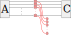
\includegraphics[width=0.7\linewidth, draft=false]{qds/individual_attacks}
	\end{subfigure}
	\begin{subfigure}{\linewidth}
		\centering
		\caption{\label{fig:types_of_attack_collective}}	
		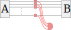
\includegraphics[width=0.7\linewidth, draft=false]{qds/collective_attacks}
	\end{subfigure}
	\begin{subfigure}{\linewidth}
		\centering
		\caption{\label{fig:types_of_attack_coherent}}	
		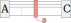
\includegraphics[width=0.7\linewidth, draft=false]{qds/coherent_attacks}
	\end{subfigure}
\caption{\label{fig:types_of_attack} Taxonomy of different eavesdropping attack strategies \cite{Lutkenhaus2004}. Black arrows denote quantum signal states distributed from Alice to Charlie. Red items belong to Bob. (a) Individual attack. Bob inserts separate probes (red boxes) into state distribution and performs measurement on each system individually. (b) Collective attack. Bob inserts separate probes into state distribution and stores his states until the end of signal distribution. He may then perform a measurement on his entire system. (c) Coherent attack. Bob interacts with all signals at the same time and he can perform a measurement on a single, global, probe. Attack (a) cannot introduce correlations between signals. Attack (b) may introduce classical correlations, and attack (c) may introduce any correlations between signals.}
\end{figure}

In this section we will focus on individual and collective forging attacks. Full security against coherent quantum attacks in the CV QKD literature has only been proven for the simpler case of coherent states modulated with a Gaussian distribution \cite{Lodewyck2007, Leverrier2010c, Pirandola2008, Leverrier2015, Laudenbach2017, Furrer2012}, and a full security proof remains elusive for a discrete modulation. There has been some recent success in applying convex optimization methods to the problem \cite{Ghorai2019, Lin2019}, but these proofs rely on an assumption about the Gaussianity of the discretely modulated alphabet \cite{Leverrier2009} which is only strictly valid in the limit $\alpha \rightarrow 0$. In keeping with recent trends in the QKD literature for discretely modulated coherent states without the assumption of Gaussianity \cite{Papanastasiou2018},  we will focus on bounding the attack strength of individual attacks, and then assume the i.i.d. criterion \cite{Leverrier2017, Laudenbach2017} in order to reach security against collective attacks. 


In particular, we will study both a beamsplitter attack and an entangling cloner attack for our protocol \cite{Grosshans2002, Grosshans2003}. In both of these attacks, Bob will replace the quantum distribution channel with a beamsplitter intended to mimic the effect of the channel on Charlie's measurement. Since Bob chooses his beamsplitter, he can do so without alerting Alice and Charlie to his presence, and so all channel loss must be attributed to Bob. Bob will either leave the second beamplitter input port empty, or he will mimic channel thermal noise by injecting there a thermal state Eq.~\ref{eqn:intro_thermal}, or one arm of his entangled two-mode squeezed vacuum state Eq.~\ref{eqn:intro_tmsv}. This so-called ``entangling cloner" attack allows Bob to gain additional information which is stored in the correlations between his two modes. This is known to be a dishonest player's optimal attack strategy in asymptotic QKD with Gaussian-modulated coherent states \cite{Lodewyck2007, Laudenbach2017}, while the optimal attack strategy against discrete-modulated QKD remains an open question. However, we conjecture that entangling cloner should be optimal in the Gaussian limit $\alpha \rightarrow 0$, and close to optimal for the small amplitudes $\alpha$ considered in this thesis. Certainly, performing an entangling-cloner attack on each signal state as it passes will be physically demanding for Bob.

\subsection{Beamsplitter attack}

\begin{figure}[htp]
\captionsetup{width=0.8\linewidth}
\centering
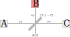
\includegraphics[draft=False,width=0.8\linewidth]{qds/BS0}
\caption{\label{fig:bs0_attack} Attack BS$0$. Bob replaces the channel with a lossless channel, plus a beamsplitter. By inputting vacuum $\dyad{0}$ into the beamsplitter, Bob mimics channel loss while imposing zero excess noise.}
\end{figure}

In its canonical form, the beamsplitter attack, Fig.~\ref{fig:bs0_attack}, allows Bob to replace a lossy channel, transmission $T$, with a corresponding lossless channel and beamsplitter. Bob inputs vacuum $\ket{0}$ into the unused input port. Bob receives his quantum system $\rho_B$ from the reflected output port, and from $\rho_B$ he will attempt to gain information about Charlie's measurement outcomes. Crucially, to honest players Alice and Charlie this attack is indistinguishable from simply having a lossy transmission channel, and so in analysis all channel loss must be attributed to the action of the dishonest Bob.  This attack cannot model any channel thermal noise, which should therefore be ignored in the analysis. A realistic channel will, however, impose noise onto Charlie's measurement outcomes, and later we describe some modificaions to the beamsplitter attack to include this.


\subsubsection{BS$0$: $\xi = 0$}\label{sec:qds_bs0}
Attack BS$0$ is depicted in Fig.~\ref{fig:bs0_attack}. This attack is the canonical beamsplitter attack, in which Bob will replace the channel with a lossless channel plus a beamsplitter. Crucially, the beamsplitter is chosen so that it mimics the channel exactly, and honest players should be unable to tell whether an attack has taken place. In a run of the protocol, therefore, all channel loss is attributed to dishonest Bob.


Consider a single input coherent state $\dyad{\alpha_k}$, with the $\alpha_k$ chosen uniformly at random from the QPSK alphabet ($k = 0,1,2,3$). Bob's attack effectively inputs the vacuum state $\dyad{0}$ into the second input port of the beamsplitter. We will calculate the Holevo information $\chi$, Eq.~\ref{eqn:intro_holevo}, of Bob's state conditioned on Charlie receiving a particular eliminated signature element after his heterodyne measurement.

Using beamsplitter relation Eq.~\ref{eqn:intro_beamsplitter} (c.f. Appendix~\ref{appendix:crypto_numerical_methods}), we see that a beamsplitter with transmission $T$ enacts the following transformation on the input state:
\begin{equation}\label{eqn:qds_coherent_state_beamsplitter}
\dyad{\alpha_k}_A \otimes \dyad{0}_B \rightarrow \dyad{\sqrt{T} \alpha_k}_C \otimes \dyad{\sqrt{1-T}\alpha_k}_{B}.
\end{equation}
So Charlie holds the state $\dyad*{\sqrt{T}\alpha_k}$, while Bob holds $\dyad*{\sqrt{1-T}\alpha_k}$. When the $\alpha_k$ is chosen uniformly at random, we must mix over the alphabet and so the mixed two-mode output state is
\begin{align}\label{eqn:qds_after_channel}
\left(\frac{1}{4}\sum_{\alpha_k} \dyad{\alpha_k}_A\right) &\otimes \dyad{0}_B \rightarrow \notag \\
&\frac{1}{4}\sum_{\alpha_k} \left(\dyad{\sqrt{T}\alpha_k}_C \otimes \dyad{\sqrt{1-T}\alpha_k}_B\right).
\end{align}

\noindent Charlie heterodynes on his mode and receives outcomes $\left(q_{\text{out}, C}, p_{\text{out}, C} \right)$. We write $z_C = q_{\text{out}, C} + i p_{\text{out}, C}$, and so Bob now holds
\begin{equation}\label{eqn:qds_bob_conditional_state}
\rho_{\left. B \given z_C \right.} = \frac{1}{4}\frac{1}{\text{P}\left(z_C\right)}\sum_{\alpha_k} \text{P}\left(z_C \given \alpha_k, T\right) \times \dyad{\sqrt{1-T}\alpha_k}_B.
\end{equation}
Here $\text{P}\left(z_C \given \alpha_k, T\right) = \left| \langle z_C | \sqrt{T}\alpha_k\rangle \right|^2$ corresponds to the probability that Charlie measures $z_C$ on his mode given that he received state $\dyad*{\sqrt{T}\alpha_k}$, while $\text{P}\left(z_C\right) = \sum_{\alpha_k} \text{P}\left(z_C | \alpha_k, T\right)$ corresponds to the total unconditional probability that he measures $z_C$.

Recall that the eliminated signature element held by Charlie is determined entirely by his heterodyne outcome $z_C$, Fig.~\ref{fig:qds_elimsig2}. Since Holevo information $\chi$ is defined in terms of Charlie's eliminated signature element rather than heterodyne measurement outcome, and since many outcomes $z_C$ will return the same eliminated signature element, we must now mix $\rho_{\left. B \given z_C \right.}$ over entire quadrants in phase-space.

\begin{figure}[htp]
\captionsetup{width=0.8\linewidth}
\centering

\includegraphics[draft=false, width=0.98\linewidth]{qds/elimsig2}
\caption{\label{fig:qds_elimsig2} Multiple heterodyne outcomes give rise to the same eliminated signature element. (a) A particular eliminated signature element. (b) All possible heterodyne outcomes consistent with (a).}
\end{figure}



Let us use the notation for eliminated signature elements from Tab.~\ref{tab:elimsig}, and consider the first eliminated signature element $e_1$. We mix $\rho_{\left. B \given z_C \right.}$ over all outcomes $z_C$ which are consistent with $e_1$, i.e. $\qout > 0$ and $\pout > 0$:

\begin{equation}\label{eqn:qds_aposterioristate}
\rho_{\left. B \given e_1\right.} = \frac{1}{\mathcal{N}\left(e_1\right)} \int\limits_{\qout>0, \pout>0} \Diff2 z_C \; \text{P}\left(z_C\right) \; \rho_{\left. B \given  z_C\right.},
\end{equation}
with the normalization factor\footnote{Clearly the normalization factor $\mathcal{N}$ as defined in Eq.~\ref{eqn:qds_aposterioristate_normalization} is equal to $1/4$ for each $e_1, e_2, e_3, e_4$. We explicitly show the general form for Eq.~\ref{eqn:qds_aposterioristate_normalization} here for completeness, though, as it will become important in Sec.~\ref{sec:qds_postselection} when we discuss postselection on measurement outcomes, and in Ch.~\ref{chapter:aqc} when assumptions about uniform sending probabilities are relaxed.} defined as
\begin{equation}\label{eqn:qds_aposterioristate_normalization}
\mathcal{N}\left(e_1\right) = \int\limits_{\qout>0, \pout>0} \Diff2 z_C \; \text{P}\left(z_C\right).
\end{equation}

\noindent The conditional state $\rho_{\left. B\given e_1\right.}$ is the quantum state held by Bob when Charlie has received eliminated signature element $e_1$. Bob's states conditioned on eliminated signature elements $e_2, e_3, e_4$ are calculated likewise by varying the limits of integration.

Bob's \emph{a posteriori} entropy, in terms of Von Neumann entropy $S$, reads
\begin{equation}
S_{\text{aposteriori}} = \sum_{e_k} \text{P}\left(e_k\right) S\left(\rho_{\left. B \given e_k\right.}\right).
\end{equation}
In this chapter we are working in the ideal case where each eliminated signature element is equally likely, and where the entropies of each of the $\rho_{\left. B \given e_k\right.}$ are equal, and so we may simply write Bob's \emph{a posteriori} entropy as

\begin{equation}\label{eqn:aposteriori_entropy}
S_{\text{aposteriori}} = S\left(\rho_{\left. B \given e_1\right.}\right).
\end{equation}

\noindent Bob's \emph{a priori} state is given by
\begin{equation}\label{eqn:qds_aprioristate}
\rho_{\text{apriori}} = \sum_{e_k} \text{P}\left(e_k\right) \rho_{\left. B \given e_k\right.}
\end{equation}
and the corresponding \emph{a priori} entropy is simply $S\left(\rho_{\text{apriori}}\right)$. Finally, using the definiition of Holevo information, Eq.~\ref{eqn:intro_holevo},
\begin{equation}\label{eqn:qds_deriv_holevo}
\chi = S_{\text{apriori}} - S_{\text{aposteriori}}.
\end{equation}
We calculate and plot $\chi$ under attack BS$0$ in Fig.~\ref{fig:qds_holevo_comparisons}. 

\subsubsection{BS$1$: $\xi > 0$}\label{sec:qds_bs1}
\begin{figure}[htp]
\centering
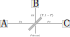
\includegraphics[draft=False, width=0.8\linewidth]{qds/BS1}
\caption{\label{fig:bs1_attack} Attack BS$1$. The beamsplitter mimics channel loss, while mixing with thermal state $\rho_{\text{thermal}}$ introduces excess noise into Charlie's outcome.}
\end{figure}
Next, let us consider a modification to attack BS$0$ which will allow us to model lossy channels which also induce excess noise in Charlie's measurement outcomes. In the first modification, denoted BS$1$ and displayed in Fig.~\ref{fig:bs1_attack}, Bob inputs a thermal state $\rho_{\text{thermal}}$, Eq.~\ref{eqn:intro_thermal}, into the second input port of the beamsplitter. This will induce excess noise $\xi > 0$ in Charlie's measurement outcomes consistent with the thermal channel noise,
where we define the excess noise in Charlie's $q$ quadrature, when coherent state $\ket{\alpha_k}$ was sent, as
\begin{equation}
\xi_q = \text{Var}\left(\qout \given \alpha_k\right) - \frac{1}{2},
\end{equation}
and similarly for $p$ quadrature. In other words, the excess noise in the $q$ quadrature is defined as the quadrature variance above the vacuum variance, and similarly for $p$. The total excess noise $\xi$ is then taken to be
\begin{equation}
\xi = \max \left\{ \xi_q, \xi_p\right\},
\end{equation}
and should be attributed to the action of dishonest Bob. We will calculate Bob's Holevo information under this attack.

We wish to mix a coherent state $\rho_{\alpha_k} = \dyad{\alpha_k}$ and a thermal state $\rho_{\text{thermal}}$ on a beamsplitter with transmission $T$. In Fock basis our states take the following form:

\begin{align}
&\rho_{\alpha_k} = e^{-\left|\alpha_k\right|^2} \sum_{n, m=0}^{\infty} \frac{\alpha_k^n \alpha_k^{* m}}{\sqrt{n! m!}} \dyad{n}{m} \notag \\
&\rho_{\text{thermal}} = \left(1 - e^{-\tilde{\beta}}\right) \sum_{p=0}^\infty e^{- p \tilde{\beta}}\dyad{p} \qq{with} \tilde{\beta} = \log_e\left(\frac{1}{\bar{n}} +1\right)
\end{align}

\noindent where $\alpha_k^{*}$ denotes the complex conjugate of $\alpha_k$. The input state into the beamsplitter is
\begin{equation}\label{eqn:qds_bs1_input_state}
\rho_{\text{input}} = \rho_{\alpha_k} \otimes \rho_{\text{thermal}}.
\end{equation}

\noindent Enacting beamsplitter relation Eq.~\ref{eqn:intro_beamsplitter_fock} on $\rho_{\text{input}}$, and heterodyning on Charlie's mode, we arrive at Bob's conditional output state $\rho_{\left. B \given z_C \right.}$. The state is displayed in full in Eq.~\ref{eqn:appendix_bs1_state}, Appendix.~\ref{appendix:bs1}.



Now, to reach the \emph{a posteriori} state under this attack we will integrate this $\rho_{\left. B \given z_C \right.}$ over all $z_C \in \mathbb{C}$ consistent with a particular eliminated signature element. Mathematically, this corresponds to simply integrating scalar terms involving $z_C$ in Eq.~\ref{eqn:appendix_bs1_state}, noting that the integration operation commutes with the rest of the state. Writing $z = z_C$ for convenience, the required integration is

\begin{equation}
\text{I}_{\text{BS}1} = \int\limits_{\qout>0, \pout>0} \Diff2 c \; z^k z^{* l} e^{ - \left| z \right|^2}
\end{equation}

\noindent where $k, l = 0, 1, 2, \dots$.

The integration is best performed in polar coordinates since the radial and angular integrals separate. We find
\begin{equation}\label{eqn:qds_bs1_deriv_3}
\text{I}_{\text{BS}1} =
\begin{cases}
\frac{\pi}{4} \Gamma\left(k+1\right) & \text{if } k = l; \\
\frac{-i}{k-l}\left(-1 + e^{i \frac{\pi}{2}\left(k-l\right)}\right)\frac{1}{2}\Gamma\left(\frac{1}{2}\left(k + l + 2\right) \right) & \text{if } k \ne l
\end{cases}
\end{equation}
with $\Gamma$ the gamma function \cite{mathworld_gamma}. Indeed, the radial component of the integrand of Eq.~\ref{eqn:qds_bs1_deriv_3} is a standard integral for $\Gamma$. The final \emph{a posteriori} state is now accessible by substituting Eq.~\ref{eqn:qds_bs1_deriv_3} into Eq.~\ref{eqn:appendix_bs1_state}.

The \emph{a priori} state is calculated likewise, but the limits of integration should be extended to the entire complex plane. In this case,
\begin{equation}\label{eqn:qds_bs1_deriv_4}
\int\limits_{\mathbb{C}} \Diff2 c \; e^{-\left|z\right|^2}z^k z^{* l} = \pi \Gamma\left(k+1\right)
\end{equation}
since the polar integral forces $k=l$. The Holevo information may now be calculated in the same way as Sec.~\ref{sec:qds_bs0} by the difference of \emph{a priori} and \emph{a posteriori} entropies, and we compare Holevo information under different attacks in Fig.~\ref{fig:qds_holevo_comparisons}.
%\MT{where do I want to talk about truncating matrices and numerical methods?}



\subsection{Entangling-cloner attack}\label{sec:qds_ec}
\begin{figure}[htp]
\captionsetup{width=0.8\linewidth}
\centering
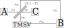
\includegraphics[draft=False, width=0.8\linewidth]{qds/EC}
\caption{\label{fig:ec_attack} EC attack. Locally, one mode of the TMSV looks like $\rho_{\text{thermal}}$ and so allows channel excess noise to be emulated. Bob can exploit correlations in noise between his two mode output state $\rho_{B_1^\prime, B_2}$ to gain additional information.}
\end{figure}
The entangling cloner attack \cite{Grosshans2002, Grosshans2003}, depicted in Fig.~\ref{fig:ec_attack}, is ideally suited to consistently incorporate the presence of excess noise $\xi$, and we shall see that it is a much more powerful attack than any of the beamsplitter attacks considered above. The entangling cloner attack, which we shall denote EC, may be viewed as a natural extension of attack BS$1$.  %EC is known to be the optimal collective attack for

Instead of inputting a thermal state into the beamsplitter's fourth port, Bob will input one arm of his entangled two-mode squeezed vacuum (TMSV) state, Eq.~\ref{eqn:intro_tmsv}. The mode which Bob inputs into the channel is locally indistinguishable from $\rho_{\text{thermal}}$, and so honest players are unable to distinguish between BS$1$, BS$2$ and EC.

%The $EC$ attack has a long history, and is known to be the optimal collective attack for gPSK QKD \MT{cite a bunch of stuff}. Since our QPSK alphabet is non-Gaussian we make no claims as to $EC$'s optimality, though we conjecture that $EC$ will be optimal as $\alpha \rightarrow 0$, and close to optimal for $\alpha << 1$. The status of optimal attacks on QDS is an open one and should be the subject of further exploration. The question about optimal attacks on QKD with discrete modulated coherent states is also open, despite a long history of activity on these protocols. In any case, the $EC$ attack is very difficult to perform with today's technology, and so a protocol with security against $EC$ (or even $BSx$) attacks should be expected to be practically secure for a long time.

%\MT{Talk somewhere about where the extra power in the EC attack comes from - we allow Bob to exploit also the correlations between his two modes. Also have some figures of histograms of this attack}

Let us analyse the EC attack. Alice creates the coherent state $\dyad*{\alpha_k}$, while Bob generates
\begin{equation}\label{eqn:qds_ec_tmsv}
\tmsv = \frac{1}{\cosh^2 \zeta}  \sum_{n, m=0}^\infty \left(\tanh\zeta\right)^{n+m} \dyad{n, n}{m, m}.
\end{equation}

\noindent Let us write the three-mode input state to the channel as

\begin{align}
\rho_{\text{input}} &= \frac{e^{-\left|\alpha_k\right|^2}}{\cosh^2 \zeta} \sum_{n_1, m_1=0}^\infty \sum_{n_2, m_2=0}^{\infty} \frac{\alpha_k^{n_1} \overline{\alpha_k}^{m_1}}{\sqrt{n_1! m_1!}} \left(\tanh\zeta\right)^{n_2 + m_2} \notag \\
&\times \bigg[\dyad{n_1, n_2}{m_1, m_2}\bigg] \otimes \dyad{n_2}{m_2},
\end{align}

\noindent where we have explicitly separated in square brackets the two modes which will interfere on the beamsplitter.

The beamsplitter mixes $\dyad{n_1, n_2}{m_1, m_2}$ via Eq.~\ref{eqn:intro_beamsplitter}, and gives an entangled three-mode state at the output. Charlie heterodynes on his mode and receives outcome $z_C$, and we arrive at Bob's conditional two-mode output state $\rho_{\left. B \given z_C\right.}$, which we display fully in Eq.~\ref{eqn:appendix_ec_state}, Appendix.~\ref{appendix:ec_state}. %A histogram of Bob's conditional two-mode state is displayed in Fig.~\ref{fig:appendix_qds_ec_histogram} where we see that his state depends heavily on Charlie's outcome $c$.  TODO: Put this sentence and the figure in the appendix

Once again the state is readily integrated in $z_C$, either over the entire complex plane or a single quadrant, and we may simply substitute Eqs.~\ref{eqn:qds_bs1_deriv_3},~\ref{eqn:qds_bs1_deriv_4} into Eq.~\ref{eqn:appendix_ec_state} to reach the \emph{a posteriori} and \emph{a priori} states, respectively.

The \emph{a priori} state is automatically normalized by virtue of the integration over $\mathbb{C}$, while the \emph{a posteriori} state is normalized by multiplying by $\mathcal{N}\left(e_1 \given \xi \right)$, defined as 

\begin{equation}
\mathcal{N}\left(e_1 \given \xi\right) = \int\limits_{\qout>0, \pout>0} \Diff2 c \; \text{P}\left(z_C \given \xi \right).
\end{equation}
where we have included excess noise $\xi$ in our probability, as in Appendix.~\ref{appendix:noisy_perr}. The performance of this attack is analysed in Fig.~\ref{fig:qds_holevo_comparisons}.


\subsection{Comparison of attacks}

We compare attacks BS$0$, BS$1$ and EC in Fig.~\ref{fig:qds_holevo_comparisons} as amplitude $\alpha$ and channel transmission $T$ are varied. We observe that for all $\alpha, T$ and for all channel thermal photon numbers $\bar{n}$ the EC attack performs best, while attack BS$1$ performs worse than even attack BS$0$ where no excess noise is considered. Under EC, Bob is permitted to exploit correlations between his two modes, and the $\bar{n}$ restricts the level of entanglement between his modes. Larger $\bar{n}$ means greater entanglement, and so we should expect that as $\bar{n}$ increases Bob gains more information. However, under BS$1$ Bob is not permitted to use these correlations, and so his outcomes and Charlie's outcomes are both noisy. The added noise reduces Bob's information without providing him the advantage of EC. 

The thermal photon number $\bar{n}$ is related to the inverse temperature of the input thermal state in BS$1$ as \cite{Leonhardt2010}
\begin{equation}
\beta = \log_e\left(\frac{1}{\bar{n}} + 1\right),
\end{equation}
while $\bar{n}$ is related to the squeezing parameter $\zeta$ of the input TMSV state in EC as \cite{Leonhardt2010}
\begin{equation}
\zeta = \text{Sinh}^{-1}\left(\sqrt{\bar{n}}\right).
\end{equation}

\begin{figure}[htp]
\captionsetup{width=0.8\linewidth}
\centering
	\begin{subfigure}{0.7\linewidth}
		\centering
		\caption{\label{fig:qds_holevo_comparisons_varalpha}}
		\includegraphics[draft=false, width=\linewidth]{qds/holevo_comparisons_varalpha}
	\end{subfigure}
	\begin{subfigure}{0.7\linewidth}
		\centering
		\caption{\label{fig:qds_holevo_comparisons_varT}}
		\includegraphics[draft=false, width=\linewidth]{qds/holevo_comparisons_varT}	
	\end{subfigure}
	\caption{\label{fig:qds_holevo_comparisons} Comparison of Holevo information $\chi$ under attacks BS$0$ (black), BS$1$ (orange) and EC (red). BS$0$ has no excess noise in the channel which corresponds to channel thermal photon number $\bar{n} = 0$. BS$1$ and EC both include excess noise, with $\bar{n} = 0.01$ (solid red/orange lines) and $\bar{n} = 0.02$ (dashed red/orange lines). (a) Increasing amplitude $\alpha$ of the QPSK alphabet leads to larger Holevo information for dishonest Bob. Honest players should therefore choose small $\alpha$. (b) At $T=0$ and $T=1$ Bob gains no information about Charlies outcomes. In both (a) and (b), we see that EC attack gives Bob much more information than BS$0$, while BS$1$ performs worse.}
\end{figure}

Since under attack BS$1$ Bob performs worse than BS$0$, we are led to consider an attack which can be considered mid-way between the power of BS$0$ and EC. We modify the attack by imposing that the channel excess noise should \emph{only} affect honest players. That is, the presence of $\xi$ causes $\perr$ to increase, but Holevo information and therefore $\pe$ should both be unaffected. We call this attack BS$2$. While strictly this attack is physically inconsistent, and therefore impossible for Bob to perform, it is more pessimistic for honest players than either BS$0$ or BS$1$ and so the security bounds it gives are also safe bounds on both of those attacks. Indeed, since an analytic expression for Bob's states under attack BS$0$ is readily attainable without resort to the numerical methods required for BS$1$ (Appendix~\ref{appendix:crypto_numerical_methods}), in some circumstances it may even be computationally preferable to assume attack BS$2$. The Holevo information is given by using Eqs.~\ref{eqn:qds_aposterioristate} and \ref{eqn:qds_aprioristate} in the usual way, while $\perr$ is given in Appendix~\ref{appendix:noisy_perr}.


\clearpage
\section{Signature length $L$}\label{sec:qds_siglength}
%\MT{better segue}
We have proven protocol security against both repudiation (Sec.~\ref{sec:qds_security_repudiation}) and forgery (Sec.~\ref{sec:qds_security_forgery}). and we have shown that our QDS protocol is robust (Sec.~\ref{sec:qds_security_robustness}). Additionally, we have demonstrated how a forging Bob's probability $\pe$ to introduce a mismatch into his signature is related to the Holevo information $\chi$ of his quantum system (Sec.~\ref{sec:qds_bounding_pe}) and have explicitly analysed several attacks which he may perform which mimic different channel conditions (Sec.~\ref{sec:qds_attack_analysis}). We are now in a position to calculate the total probability that our QDS protocol fails to meet the security requirements outlined in List.~\ref{list:qds_requirements}. We shall see that the total failure probability decays exponentially, and so our protocol is secure.

Let us define $\varepsilon_{\text{fail}}$ as the total probability that our protocol fails, either by allowing a repudiation or forging attack, or by aborting when all players behaved honestly. To gain a figure of merit we assume that the protocol is equally likely to fail in any of these ways, and so we set
\begin{equation}\label{eqn:qds_efail_deriv}
\varepsilon_{\text{fail}} = \varepsilon_{\text{honest abort}} = \varepsilon_{\text{repudiation}} = \varepsilon_{\text{forgery}},
\end{equation}
though we note that alternative combinations may be easily considered. Let us eliminate the free parameters $s_B, s_C$ by equating the arguments of Eqs.~\ref{eqn:erep},~\ref{eqn:ehonabort}, \ref{eqn:eforg}:
\begin{equation}
\left(\pe - s_C\right)^2  = \frac{1}{4}\left(s_C - s_B\right)^2 = \left(s_B - \perr\right)^2,
\end{equation}
from which we may derive
\begin{equation}\label{eqn:qds_sbsc}
s_B = \frac{3}{4} \perr + \frac{1}{4}\pe \qq{and} s_C = \frac{1}{4}\perr + \frac{3}{4}\pe,
\end{equation}
as our choices of security thresholds. Notice that since $\perr \le \pe$, Eq.~\ref{eqn:qds_sbsc} automatically fulfils the requirement that $s_B \le s_C$. The overall probability of failure Eq.~\ref{eqn:qds_efail_deriv} therefore becomes

\begin{equation}\label{eqn:efail}
\varepsilon_{\text{fail}} \le 2 \text{exp}\left( - \left[\pe - \perr\right]^2 \frac{L}{16}\right).
\end{equation}

\noindent This probability $\varepsilon_{\text{fail}}$ decays exponentially in $L$, and so provided that $\perr$ and $\pe$ are known, and $\pe - \perr \ge 0$, any security level $\varepsilon_{\text{fail}} > 0 $ may be reached by varying signature length $L$. In keeping with the recent works Refs.~\cite{Collins2014, Croal2016, Donaldson2016, Amiri2016} in this Thesis we will take $\varepsilon_{\text{fail}} = 0.01\%$. Equation~\ref{eqn:efail} may then be solved for the signature length. We take $L$ as the main figure of merit\footnote{Analogously to the key rate in QKD.} for a QDS protocol, and analyse the performance of our protocol in Sec.~\ref{sec:qds_protocol_performance}.



\section{Postselection}\label{sec:qds_postselection}
In the context of QKD it has been known for some time that a postselection of measurement outcomes, in which measurement outcomes unfavourable to honest players are discarded, will improve the key rates in the presence of excess noise. Postselection is even a requirement to distill a key below $T \le 1/2$ in the direct reconciliation regime \cite{Silberhorn2002}. We are thus motivated to apply postselection to our QDS protocol in order to allow a message to be securely signed over a larger range of channel parameters, and we shall see that it can reduce the necessary $L$. The results of this section will be especially useful in Ch.~\ref{chapter:aqc} where -- as for direct reconciliation QKD -- we shall see that postselection is a necessity for some QDS protocols.

For now, we will apply postselection to the protocol outlined in this chapter. To apply the postselection technique, recipients Bob and Charlie will simply disregard unfavourable measurement outcomes, i.e. outcomes for which a dishonest player is deemed to have too much knowledge, or for which the probability of honest mismatch is too high.

We define a region $\rps \in \mathbb{C}$, Fig.~\ref{fig:rps}. Honest recipients will only accept measurement outcomes $\left(\qout, \pout\right)$ with $c := \qout + i \pout \in \mathbb{C}\setminus\rps$. We may then vary $\rps$ in order to increase the range of channel parameters for which the QDS protocol is secure, and to minimize signature length $L$.

\begin{figure}[htp]
\captionsetup{width=0.8\linewidth}
\centering
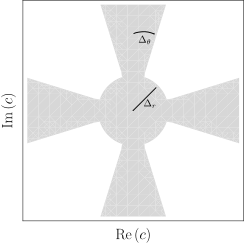
\includegraphics[draft=false, width=0.7\linewidth]{qds/rps2}
\caption{\label{fig:rps} The postselection region $\rps$, gray, is parametrized by $\Delta_r, \Delta_\theta$ in polar coordinates. Participants will only accept measurement outcomes $c \in \mathbb{C} \setminus \rps$. }
\end{figure}

Our chosen $\rps$ is parametrized by two variables $\Delta_r, \Delta_\theta$ in polar coordinates, Fig.~\ref{fig:rps}. This is the same postselection region which was considered in the recent work Ref.~\cite{Lin2019}, but if desired more general regions may be readily considered. We make no claims as to the optimality of our choice of the shape $\rps$, though once the form of $\rps$ is set we may optimize over $\Delta_r$ and $\Delta_\theta$ to improve protocol security.

The crucial quantity which controls the security of our QDS protocol is $g_{\text{sec}} := \pe - \perr$, which describes how much more likely a dishonest player is to induce a mismatch than an honest player. We saw in Sec.~\ref{sec:qds_siglength} that our QDS protocol is secure provided that $g_{\text{sec}} > 0$, and that the signature length $L$ required to sign to a given level of security $\varepsilon_{\text{fail}}$ is directly controlled by $g_{\text{sec}}$. We therefore must consider how postselection affects $g_{\text{sec}}$. 

Let us begin with the effect of postselection on $\perr = \perr\left(\Delta_r, \Delta_\theta\right)$. %\MT{I don't want to talk yet about calculating $\perr$ from data - that should wait until the agile chapter.} 
Recall that when Alice sends state $\ket{\alpha}$ through a lossy but noiseless channel, transmission $T$, Charlie receives $c \in \mathbb{C}$ with probability

\begin{equation}
\text{P}\left(c \given \alpha, T\right) = \frac{1}{\pi} \exp\left( - \left| c - \sqrt{T}\alpha\right|^2\right).
\end{equation}

\noindent Thus the probability of eliminating the state $\ket{\alpha}$ when no postselection is used is, in polar coordinates,
\begin{align}\label{eqn:perrps_deriv_nops}
\perr &= \int\limits_{r=0}^\infty \mathrm{d}r \; r \int\limits_{\theta = \pi/2}^{3 \pi/2} \mathrm{d}\theta \; \text{P}\left(r e^{i \theta} \given \alpha, T\right) \notag \\
%
&= \frac{1}{2}\erfc\left(\sqrt{\frac{T}{2}}\left|\alpha\right|\right).
\end{align}

\noindent When the postselection technique is used we must change the limits of integration, so the mismatch probability becomes

\begin{align}\label{eqn:perrps_deriv_2}
\perr\left(\Delta_r, \Delta_\theta\right) %= \frac{1}{\mathcal{N}} \int\limits_{\left.x \in \mathbb{C} \setminus \rps \given \text{Re}\left(x\right) < 0\right. } \Diff2 x \; \text{P}\left(x \given \alpha, T\right) \notag \\
= \frac{1}{\mathcal{N}} \int\limits_{\Delta_r}^{\infty} \mathrm{d}r \; r &\left[ \; \int\limits_{ \pi/2 + \Delta_\theta}^{\pi - \Delta_\theta} \mathrm{d}\theta \; \text{P}\left(r e^{i \theta} \given \alpha, T\right) \right. \notag \\
%
 &+ \left. \int\limits_{3 \pi/2 - \Delta_\theta}^{\pi + \Delta_\theta} \mathrm{d}\theta \; \text{P}\left(r e^{i \theta} \given \alpha, T\right) \right],
\end{align}


\noindent where we effectively have the same integrals as Eq.~\ref{eqn:perrps_deriv_nops} restricted by $\rps$. The normalization probability $\mathcal{N}$ is the probability that Charlie will accept his measurement outcome, which is calculated by extending the integration in Eq.~\ref{eqn:perrps_deriv_2} to the entire $\mathbb{C} \setminus \rps$

\begin{equation}\label{eqn:qds_perrps_normalization}
\mathcal{N} = \int\limits_{\mathbb{C} \setminus \rps} \Diff2 c \; \text{P}\left(c \given \alpha, T, \xi \right).
\end{equation}

\noindent The calculation of $\perrps$ follows identically to Eq.~\ref{eqn:perrps_deriv_2} when excess noise $\xi$ is included, simply using the requisite formula (Appendix~\ref{appendix:noisy_perr}) and performing the integrations as Eq.~\ref{eqn:perrps_deriv_2}.


Since a dishonest player's declaration will depend on an honest player's heterodyne outcome, the probability $\pe$ must also vary with $\rps$. We will calculate the effect of $\rps$ on Holevo information $\chi$, from which the probability $\pe$ is calculated via Eq.~\ref{eqn:qds_hpe} as normal.

%Let Bob's $j^{\text{th}}$ \emph{a posteriori} state be $\rho_{B | e_k}^j$, which is conditioned on Charlie holding eliminated signature element $e_k$. 
Assume that Bob has performed any one of the attacks examined in Sec.~\ref{sec:qds_attack_analysis}, and let Bob's state after Charlie's heterodyne measurement be denoted $\rho_{\left. B \given c\right.}^j$. Again, since Charlie's eliminated signature element is entirely determined by the quadrant in which $c$ lies, the state $\rho_{\left. B \given  e_k\right.}^j$ is calculated by mixing $\rho_{\left.B \given c\right.}^j$ over an entire quadrant of phase-space, as in Eqs.~\ref{eqn:qds_aposterioristate},~\ref{eqn:qds_bs1_deriv_3}, Tab.~\ref{tab:elimsig}. We must therefore update these integrals to include the effect of $\rps$. For example,

\begin{align}\label{eqn:qdsps_aposteriori}
\rho_{\left.B \given e_1\right.}^j = \frac{1}{\mathcal{N}} \int \Diff2 c \; \rho_{\left. B \given c\right.}^j
%
=\frac{1}{\mathcal{N}} \int\limits_{\Delta_r}^\infty \mathrm{d}r\; r\int\limits_{\Delta_\theta}^{\pi/2 - \Delta_\theta} \mathrm{d}\theta \; \rho_{\left. B \given r e^{i \theta}\right.},
\end{align}

\noindent and similarly for $e_2, e_3, e_4$. The $\mathcal{N}$ is identical to that required for Eq.~\ref{eqn:perrps_deriv_2}, and Bob's $\emph{a priori}$ state is found by mixing Eq.~\ref{eqn:qdsps_aposteriori} over all quadrants. Probability $\pe\left(\Delta_r, \Delta_\theta\right)$ may now be calculated via Eq.~\ref{eqn:qds_hpe}. 

To actually perform the integration, we separate out terms involving $c$ in Bob's state %(see Secs.~\ref{sec:qds_bs0},~\ref{sec:qds_ec},~\ref{sec:appendix_bs1_state},~\ref{sec:appendix_ec_state}) , 
and so the integration becomes

\begin{equation}
\frac{1}{\mathcal{N}} \int\limits_{\Delta_r}^{\infty} \mathrm{d}r \; r \int\limits_{\Delta_\theta}^{\pi/2 - \Delta_\theta} \mathrm{d}\theta \; r^k r^l e^{-r^2} e^{i \theta \left(k - l\right)}.
\end{equation}

\noindent where we have used $c = r e^{i \theta}$. To perform the integration, it is helpful to perform the angular integral first, which readily integrates to a sum of exponentials when $k \ne l$, or to $\pi/2 - 2\Delta_\theta$ when $k=l$. The remaining radial term is

\begin{equation}\label{eqn:qds_perrps_radial_integration}
\int\limits_{\Delta_r}^\infty \mathrm{d}r \; r^{k + l + 1} e^{-r^2}
\end{equation}

\noindent which is the definition of an upper incomplete Gamma function \cite{Mathworld_Incomplete_Gamma}, which we denote as $\Gamma_\uparrow$. The radial integration Eq.~\ref{eqn:qds_perrps_radial_integration} is thus identically

\begin{equation}
\Gamma_{\uparrow}\left(\frac{1}{2}\left[2 + k + l\right], \Delta_r^2\right)  \forall k, l \ge 0
\end{equation}
which may be easily calculated.

We have now included the effects of $\rps$ on $g_{\text{sec}}$, and so the performance of the protocol under postselection may be analysed. In Fig.~\ref{fig:qds_gsec_varying_rps} we plot $g_{\text{sec}}$ varying $\rps$ for attacks BS$0$, BS$1$, and EC, and for different coherent state amplitude $\alpha$'s at $T=0.5$. We observe that when considering $g_{\text{sec}}$, it is advantageous to choose a large postselection region as this always allows $g_{\text{sec}}$ to increase. However we also observe that the effectiveness of postselection depends on our coherent state amplitude. For example, at $\alpha=0.2$ we see smaller increase in $g_{\text{sec}}$ as $\rps$ is increased, and there is almost no effect of postselection as $\Delta_\theta$ is varied under EC attack.


\begin{figure}[htp]
\captionsetup{width=0.8\linewidth}
\centering
	\begin{subfigure}{0.7\linewidth}
		\centering
		\caption{}
		\includegraphics[draft=false, width=\linewidth]{qds/rps_varying_gsec_1}
	\end{subfigure}
	\begin{subfigure}{0.7\linewidth}
		\centering
		\caption{}
		\includegraphics[draft=false, width=\linewidth]{qds/rps_varying_gsec_2}
	\end{subfigure}
\caption{\label{fig:qds_gsec_varying_rps} The efficacy of postselection depends strongly both on attack type and parameters $\alpha, T$. Solid: $\Delta_\theta = 0$. Dashed: $\Delta_\theta = 0.3$. Green: BS$0$. Orange: BS$1$.  Red: EC. (a) $\alpha = 0.5, T=0.5$ and (b) $\alpha = 0.2, T=0.5$. In both graphs attacks BS$1$ and EC have excess noise $\xi = 0.1\%$.  }
%Calculations/Cryptography/2020-02-11_gsec_varying_rps
%Technically, blue is BS0 and Green is BS2, but they are basically overlapping and I am trying to downplay attack BS2.
%This caption originally said that \xi=0.001% but I have changed it because I think it was wrong. TODO: check
\end{figure}


Let us turn now to examine our main figure of merit, the number of quantum states $L$ used in the protocol. Directly incorporating $g_{\text{sec}}\left(\Delta_r, \Delta_\theta\right)$ into Eq.~\ref{eqn:efail} will give an erroneous level of security, for the following reason. Our calculations in this section, culminating in $g_{\text{sec}}\left(\Delta_r, \Delta_\theta\right)$, correctly bound the number of states required to sign a message to security level $\varepsilon_{\text{fail}}$. However, this is not equivalent to the number of states which Alice has actually sent. 

For example under attack EC with $\alpha=0.5, T=0.5, \xi=0.1\%$, choosing $\Delta_r = 4.0 $ and $\Delta_\theta = 0.4 $ gives $g_{\text{sec}} = 0.1225 $. Substituting this into Eq.~\ref{eqn:efail} and solving for $L$ gives $L = 10560$. But in order to have that many states accepted at Charlie, Alice will actually need to have sent $7\times10^{10}$ coherent states in total, since Charlie will reject his measurement outcomes with probability $1 - \left(1.5\times10^{-7}\right)$, Eq.~\ref{eqn:qds_perrps_normalization}. It follows that $L$, as implicitly defined by Eq.~\ref{eqn:efail}, is actually a poor figure of merit to measure the resource-use of our protocol when postselection is used.

Instead, we will work in terms of $\tilde{L}$, which we define as the total number of states sent by Alice. This may be written as a rescaling of $L$ given by
\begin{equation}
L \mapsto \tilde{L} := \frac{L}{\mathcal{N}},
\end{equation}
with the normalization factor $\mathcal{N}$ interpreted sthe average probability that Charlie accepts a given state sent by Alice, Eq.~\ref{eqn:qds_perrps_normalization}.

We plot $\mathcal{N}$ in Fig.~\ref{fig:psnorm}, and figure of merit $\tilde{L}$ in Fig.~\ref{fig:qds_L_vs_deltar}. We observe that even though large $\Delta_\theta$ causes $g_{\text{sec}}$ to increase, Fig.~\ref{fig:qds_gsec_varying_rps}, it also causes an increase in $\tilde{L}$, owing to the quick decay of $\mathcal{N}$ with $\Delta_\theta$, Fig.~\ref{fig:psnorm}. We also may deduce from the graphs Fig.~\ref{fig:qds_L_vs_deltar} that there is an optimum $\Delta_r$ which minimizes $\tilde{L}$ and gives the best performance of our protocol.


\begin{figure}[htp]
\captionsetup{width=0.8\linewidth}
\centering
\begin{subfigure}{0.4\linewidth}
\includegraphics[draft=false, width=\linewidth]{qds/psnorm1}
\caption{}
\end{subfigure}
\begin{subfigure}{0.4\linewidth}
\includegraphics[draft=false, width=\linewidth]{qds/psnorm2}
\caption{}
\end{subfigure}
\caption{\label{fig:psnorm} Normalization factor $\mathcal{N}$ Eq.~\ref{eqn:qds_perrps_normalization} varies dramatically with postselection region $\rps$. (a) $\alpha=0.5, T=0.5$. (b) $\alpha=3.0, T=1.0$}
%images/qds/psnorm.nb
\end{figure}

\begin{figure}[htp]
\captionsetup{width=0.8\linewidth}
\centering
	\begin{subfigure}{0.7\linewidth}
		\centering
		\caption{}
		\includegraphics[draft=false, width=\linewidth]{qds/rps_varying_L_1}
	\end{subfigure}
	\begin{subfigure}{0.7\linewidth}
		\centering
		\caption{}
		\includegraphics[draft=false, width=\linewidth]{qds/rps_varying_L_2}
	\end{subfigure}
\caption{\label{fig:qds_L_vs_deltar} The key figure of merit, $\tilde{L}$, depends strongly on postselection region $\rps$. Solid: $\Delta_\theta=0$. Dashed: $\Delta_\theta = 0.3$. Green: BS$0$. Orange: BS$1$. Red: EC. (a) $\alpha = 0.5, T = 0.5$ and (b) $\alpha=0.2, T=0.5$. In both graphs attacks BS$1$ and EC have $\xi = 0.1 \%$. In all cases it is optimal to choose $\Delta_\theta = 0$}
%Calculations/Cryptography/2020-02-12_L_varying_rps.nb
\end{figure}

Since the figures of merit $\tilde{L}$ (with postselection)and $L$ (without postselection) qualitatively measure the same thing -- how many states must Alice send in order to sign a $1$~bit message -- they may be directly compared. For the remainder of this Thesis, then, we will not distinguish between $\tilde{L}$ and $L$. It should be understood that when postselection is used we are using the rescaled $\tilde{L}$, while when postselection is not use we are using $L$. Furthermore, since $\Delta_\theta > 0$ causes $\tilde{L}$ to increase we will take the optimal $\Delta_\theta=0$ always from now on, and only allow $\Delta_r$ to vary. It will be made clear in what follows whether the postselection technique has been used and the choice of $\Delta_r$.



%\clearpage
\section{Protocol performance}\label{sec:qds_protocol_performance}
Let us apply the analysis performed in the previous few sections and calculate our main figure of merit, the signature length $L$, under several different attacks. We plot the signature length $L$ required to sign a $1$~bit message under attacks BS$0$ (black) and EC (red) in Fig.~\ref{fig:qds_nonoptimal_L}, for several different $\alpha$. An entangling cloner attack with $\xi = 0.1\%$ has vastly increased signature length for $\alpha=0.2$ (dotted), while for larger $\alpha=0.5, 0.8$, entangling-cloner causes the signature length to by more modest amounts when compared to BS$0$. Note that in Fig.~\ref{fig:qds_nonoptimal_L} the transmissions $T$ at which the lines stop should be interpreted as being close to the smallest $T$ attainable before $L$ begins to diverge, and signing a message becomes impractical (in the case of BS$0$) or impossible (in the case of EC). 





\begin{figure}[htp]
\captionsetup{width=0.8\linewidth}
\centering
\includegraphics[width=0.7\linewidth, draft=false]{qds/QDSf_nonoptimal_L}
\caption{\label{fig:qds_nonoptimal_L} Signature lengths $L$ varying with channel transmission $T$ for attacks BS$0$ (black) and EC (red). Solid: $\alpha=0.5$. Dashed: $\alpha=0.8$. Dotted: $\alpha=0.2$. Entangling cloner attack has excess noise $\xi = 0.1\%$ at all T. A non-optimal choice of $\alpha$ can lead to much larger signature lengths. No postselection is used.}
\end{figure}


Even when attack BS$0$ is used and $\xi=0\%$, a sub-optimal choice of coherent state amplitude $\alpha$ can drastically worsen the performance of the protocol. To investigate optimal amplitudes, we plot the security parameter $g_{\text{sec}}$ varying with $\alpha$ under attack BS$0$ in Fig.~\ref{fig:qds_gsec_croal}. We observe that the optimal $\alpha$ decreases with increasing loss (smaller $T$). Intuitively, at $T=1.0$ Eve gains no information and so one should pick $\alpha \gg 1$ so as to minimize mismatch rate between honest players. 

We also compare our current protocol to a recent CV QDS protocol \cite{Croal2016} which did not allow for the presence of an eavesdropper on the quantum channels. The security parameter under Ref.~\cite{Croal2016} is displayed as red, dot-dashed lines in Fig.~\ref{fig:qds_gsec_croal} at $T=0.47$ (top) and $T=0.19$ (bottom). We see that for larger $T$, and almost all $\alpha$ at smaller $T$, our current protocol outperforms Ref.~\cite{Croal2016}, despite our relaxing the requirement of secure quantum channels. This surprising improvement in performance comes directly from the fact that in the current protocol, Alice distributes different signatures to each recipient, whereas in Ref.~\cite{Croal2016} she distributed identical signatures.

\begin{figure}[htp]
\captionsetup{width=0.8\linewidth}
\centering
\includegraphics[width=0.7\linewidth, draft=false]{qds/Thornton2019_croal_comparisons}
\caption{\label{fig:qds_gsec_croal} Security parameter $g_{\text{sec}}$ under attack BS$0$ as it varies with $\alpha$ for $T = 0.61$, $0.47$, $0.19$, $0.11$, $0.01$ (solid, black, top to bottom). The optimal $\alpha$ which should be chosen to maximize $g_{\text{sec}}$ (minimize L) decreases as $T$ decreases. Horizontal gridlines denote $\mathcal{O}\left(L\right)$ starting from $L \sim 10^5$ at $g_{\text{sec}} = 0.038$ (top), with $L$ increasing by a factor of $10$ at subsequent lower gridlines. Red, dot-dashed: $g_{\text{sec}}$ calculated via the protocol described in Ref.~\cite{Croal2016} for $T=0.19$ and $T=0.47$.}
\end{figure}

We optimize over $\alpha$ and postselection region $\Delta_r$ in Fig.~\ref{fig:qds_optimal_L}. The figure thus represents the smallest attainable $L$ for our protocol under attacks BS$0$ (solid, blue), BS$2$ (dashed, orange) and EC (solid, red). Attack BS$1$ gives smaller $L$ than even BS$0$, and so we do not show it. Even at the $T \sim 0.4$ corresponding to a fiber length $\sim 20$~km, the attainable $L$ are very modest at only $\mathcal{O}\left(10^5\right)$ under BS$0$ and $\mathcal{O}\left(10^6\right)$ for EC attacks. 


\begin{figure}[htp]
\captionsetup{width=0.8\linewidth}
\centering
\includegraphics[width=0.7\linewidth, draft=false]{qds/QDSf_optimal_L}
\caption{\label{fig:qds_optimal_L} Signature lengths under protocols BS$0$ (blue, solid), BS$2$ (orange, dashed) and EC (red, solid). At each point $L$ is optimized over $\alpha$ and postselection parameter $\Delta_r$. EC attack with $\xi = 0.1\%$.}
\end{figure}

Finally, in Appendix~\ref{appendix:qds_larger_alphabets} we extend the protocol discussed in this chapter to allow for larger alphabet sizes. These alphabets, which we denote as $N$PSK alphabets, consist of $N$ coherent states equally distributed around the origin of phase space. The case $N=4$ is equivalent to the QPSK alphabet which we have used until now. For $N$PSK alphabets with $N=2$, $N=4$, $N=6$, $N=8$ we plot their signature lengths optimized over $\alpha$ in Fig.~\ref{fig:qds_npsk_length_body}, and the required optimal $\alpha$'s are displayed in the inset. 

Surprisingly, although for larger alphabets the optimal $\alpha$ is decreased, the minimal $L$ is slightly increased. As has been found elsewhere \cite{Leverrier2011}, the biggest leap in behaviour should occur between $2 \rightarrow 4$, and indeed this is what we see\footnote{Noting that for the case $N=2$ we no longer need to think about an eliminated signature and we may simply consider optimal guessing probabilities.}. As $N$ increases, with $\alpha \ll 1$ we tend closer towards a Gaussian mixture of coherent states (c.f. Fig.~\ref{fig:intro_npsk}b). We may therefore reasonably expect the attack strategies BS$0$ and EC to become increasingly optimal in this Gaussian limit, which explains the slight increase in $L$ for larger alphabets.

\begin{figure}[htp]
\captionsetup{width=0.8\linewidth}
\centering
\includegraphics[width=0.7\linewidth, draft=false]{qds/appendix_npsk_length}
\caption{\label{fig:qds_npsk_length_body} Signature length $L$ under attack BS$0$. At each $T$, length $L$ has been optimized over amplitude $\left|\alpha\right|$ of the alphabet. We have considered $N$PSK alphabets with $N = 2$, $4$, $6$, $8$. Dot-dashed: $N=2$. Black, solid: $N = 4$. Dashed: $N = 6$. Gray, solid: $N = 8$. Inset: the corresponding optimal $\alpha_{\text{opt}}$. } %created in "Creating graphs for paper.nb" from my PRA paper folder.
\end{figure}

\clearpage
\section{Outlook}
Quantum digital signatures, which use quantum resources to allow for secure authentication of a classical message, have only recently been proven secure against a quantum eavesdropper on the channels \cite{Amiri2016, Puthoor2016, Yin2016}. In this Chapter, we have progressed continuous-variables QDS by providing security against an eavesdropper performing one of several beamsplitter attacks, or an entangling-cloner attack, on the quantum channels. Surprisingly, short signature signature lengths are sufficient to perform secure QDS over metropolitan distances, and we require even shorter signatures than a comparable scheme in Ref.~\cite{Croal2016} which assumed secure quantum channels. Our security proof has enabled us also to take into account the fact that for each eliminated signature element there are multiple ``correct" declarations which a dishonest player can make.

Our security proof has relied on several assumptions which reflect the state-of-the-art of CV quantum cryptography with our chosen alphabet of discrete-modulated coherent states, but which future work should strive to relax. First, the eavesdropping attacks permitted by a dishonest player in this chapter do not give them the full power of quantum mechanics, and there are additional attacks which could be performed which may prove additionally effective. For example, a dishonest player could begin to induce and exploit quantum correlations between subsequent distributed states. There may also be additional attacks on individual signature elements which are more powerful than the ones considered here. The non-Gaussianity of our alphabet is restrictive, and the entangling-cloner attack is only expected to be optimal as a limiting case that the QPSK alphabet becomes Gaussian, i.e. $\alpha \rightarrow 0$ \cite{Navascues2006, Garcia-Patron2006}. One possible route towards a fuller security analysis could be an extension of results known for QKD with two-state \cite{Zhao2009} and three-state \cite{Bradler2018} alphabets to our four-state alphabet, noting recent progress in Ref.~\cite{Papanastasiou2018}. We expect that such an extension, if even possible, will be challenging.

One may begin to further consider the finite-size effects \cite{Tomamichel2016} which are intrinsic to any QDS scheme, noting the operational links between the guessing probabilities $\pe$ considered in this Chapter, and the smooth min-entropy \cite{Konig2009}. A calculation of smooth min-entropy has been used to good effect for DV QDS in Refs.~\cite{Amiri2016, Puthoor2016}, where we note that a full calculation also allows for security against coherent attacks. Advances in calculating optimal lower bounds for the smooth min-entropy under a discrete-modulated coherent state alphabet will have immediate and direct application to CV QDS, and may be readily incorporated into our security proof. Recent work \cite{Seshadreesan2017} has allowed for direct calculations of smooth min-entropy for an alphabet of Gaussian-modulated coherent states via the covariance matrix formalism, and recent QKD work \cite{Ghorai2019, Lin2019} has successfully handled the QPSK alphabet only by assuming that it is Gaussian, i.e. $\alpha \ll 1$, allowing the mixture of states to be completely described by a covariance matrix. In our case, however, choosing $\alpha$ such that this criterion is met and any bounds are tight enough to be useful, also gives very large $\perr$ rendering our protocol insecure. Further work is needed.

A fully Gaussian CV QDS protocol is conceivable, in which Alice distributes coherent states chosen from a Gaussian probability distribution. It is likely that the resulting analysis could proceed almost entirely in the covariance matrix formalism \cite{Weedbrook2012, Serafini2018}, for which good bounds for smooth min-entropy are known. One should take care in the analysis to correctly define $\perr$ however, as there is now no natural partitioning of phase-space. One may therefore also need to optimize over the best choice of phase-space partition with which to define an eliminated signature, and it will be interesting to observe how this partitioning is affected by channel parameters $T$, $\xi$, the variance of the underlying Gaussian probability distribution, and the choice of postselection region $\rps$.


The security of our QDS protocol and the short $L$ required to sign a message, stemming both from our security proof and the practical advantages of the CV platform, make CV QDS an attractive scheme for secure communications in a quantum future. We further explore this protocol in Chapter~\ref{chapter:aqc} where we investigate its practical experimental implementation alongside related cryptographic protocols. We demonstrate, there, that the short signature lengths obtained for this protocol result in small times required to sign a message in a practical implementation. Thus, to our knowledge, this QDS protocol is the fastest protocol over comparable distances.

A brief discussion of the numerical methods which are used for this current Chapter may be found in Appendix~\ref{appendix:crypto_numerical_methods}, where we also display the full quantum states used for attacks BS$0$, BS$1$ and EC.



%\MT{have an "outlook" section where I make some remarks about the postselection technique. Note that I have implicitly assumed that Bob knows whether an individual state has been postselected on. This is a sensible assumption for QKD, since it will be declared, but for QDS it does not need to be declared, so I am giving Bob too much power here.}

%%%
%
% TODO:
% - talk somewhere about the types of attack which we allow
% - make sure I talk about the types of channel which we use
% Q: where should I talk about Alice's function F?
% - understand the mapping from complex values to binary
% - some more remarks about the running of the protocol?
% - mention somewhere my linestyle convention for different types of channel

\chapter{Quantum secret sharing}
Goal of chapter: introduce our QSS protocol and prove its security in different contexts.

\iffalse
Key results which I want to present:
\begin{itemize}
\item our QSS protocol
\item security proof (what does it do? what does it not do?)
\item analysis of security in various settings - heterodyne, $\mathcal{A}_4$, BS0, BS1, BS2, EC, varying $\alpha$, $T$, $\xi$, $g$, $h$ of both channels
\item show how the protocol performs
\end{itemize}
\fi

\MT{Short introduction to chapter.}

\section{Our QSS protocol}

Our quantum secret-sharing scheme allows for a dealer, Alice, to distribute a classical secret between two recipients, Bob and Charlie. Bob and Charlie should be able to exactly reconstruct the secret when they behave honestly, while a dishonest and unauthorised conspiracy of players--including those outside the protocol--should gain no information. Crucially, although the scheme should allow for dishonesty among the recipients a dishonest player should be forced to collaborate with an honest one.

\begin{figure}[htp]
\centering
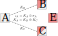
\includegraphics[draft=false, width=0.5\linewidth]{qss/qss_setup_cartoon}
\caption{\label{fig:qss_structure} All quantum secret sharing schemes follow the same structure. Alice encrypts her classical secret $\sigma_A$ with key $K_A$, and broadcasts the resulting $\varsigma_A$. Shares of $K_A$ are distributed among recipients Bob and Charlie such that $K_B \oplus K_C = K_A$. Gray boxes denote honest players, while red denotes dishonest players. The half-red/half-gray boxes denote uncertainty about which player is dishonest. %say somewhere it's all classical?
}
\end{figure}

\subsection{QSS setup}

All QSS protocols follow essentially the same structure, Fig.~\ref{fig:qss_structure}:
\begin{enumerate}
\item Alice (A) uses quantum resources to distribute shares of classical key $K_A$ among recipients Bob (B) and Charlie (C), such that $K_A = K_B \oplus K_C$.
\item Alice encrypts her secret $\varsigma_A = K_A \oplus \sigma_A$ and makes the encrypted secret $\varsigma_A$ publicly known.
\end{enumerate}
The $\oplus$ operation corresponds to bitwise addition (XOR) of binary keys and, provided that $K_A, K_B, K_C$ and $\sigma_A$ are the same length, the above secret sharing operation is provably unconditionally secure \cite{Schneier1996}, provided that key shares $K_B, K_C$ are securely distributed.

This form is similar to QKD-based encryption and it is for this reason that renowned cryptographer Gustavus Simmons wrote that 

\begin{center}\emph{``Secret sharing is simply a special form of key distribution''}\end{center}

\noindent as the abstract to Ref.~\cite{Simmons1990a}.

QSS protocols then only differ in the method used to generate and share the $K_B, K_C$ forming the encryption key. One attractive option would be for Alice to perform individual QKD protocols, first with Bob and then with Charlie, and then XOR the resulting keys together. Since QKD is provably secure, neither Bob nor Charlie can gain sufficient information about the other player's key. The resulting QSS scheme is thus also secure. We discuss this form of QSS at length in Sec.~\ref{sec:intro_qss_lit_review} and again in Chapter~\cite{chapter:aqc}.

Other options for generation and distribution of $K_B, K_C$ are discussed in Sec.~\ref{sec:intro_qss_lit_review} and fall into one of two categories. The first category \cite{Hillery1999, Karlsson1999, Gottesman1999, Markham2008, Wu2016, Kogias2017} relies on large entangled states shared between all $N$ players, while the second category \cite{Zhang2005a, Schmid2005, Schmid2007, Grice2019}, involves distribution of a single (typically one-mode) quantum state between all $N$ players, who each perform their choice of measurement on the state. In both forms, if $N-1$ players communicate and share their choice of measurement and their measurement outcomes, they have sufficient information to infer the measurement outcome of the $N^{\text{th}}$ player. In this way, a key $K_A$ is distributed between players.


\subsection{QSS protocol description}

We propose a QSS protocol which will perform the task of quantum secret sharing without requiring the distribution of highly entangled states between players \cite{Kogias2017} and without requiring a dedicated hardware or network setup \cite{Grice2019}. Instead, we rely on distribution of QPSK alphabet Eq.~\ref{eqn:intro_qpsk} and heterodyne detection Sec.~\ref{eqn:intro_heterodyne}. The QSS protocol guards against both eavesdropping by choice of QPSK alphabet with small coherent state amplitude $\alpha$, which ensures that Eve cannot accurately guess Alice's heterodyne outcomes. The protocol guards against the internal dishonesty of Bob or Charlie by ensuring that the key $K_A$ which Alice will use to encrypt her secret is a function of \emph{both} Bob and Charlie's information.% The dishonest internal player is then forced to collaborate with Eve to attack the honest player's quantum channel, which, by our choice of alphabet, will not succeed.

In our protocol, Bob and Charlie are chosen as the senders of the quantum states. This has advantage in that we may fully trust Alice's heterodyne detection\footnote{Note that permitting Bob or Charlie to perform the heterodyne detection implicitly places trust in their heterodyning beamsplitter \cite{Walk2016a}.} and its characterisation. A dishonest internal player will be forced to collaborate with Eve to attack the honest player's quantum channel. By our choice of alphabet, this will not succeed.

\begin{figure}[htp]
\centering
	\begin{subfigure}{0.8\linewidth}
		\centering
		\caption{\label{fig:qss_distribution_stage}}
		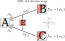
\includegraphics[draft=false, width=\linewidth]{qss/qss_distribution_stage}
		
	\end{subfigure}
	\begin{subfigure}{0.8\linewidth}
		\centering
		\caption{\label{fig:qss_encryption_stage}}
		\includegraphics[draft=false, width=\linewidth]{qss/qss_encryption_stage}
		
	\end{subfigure}
\caption{\label{fig:qss_protocol_cartoon} Distribution and encryption stages of our QSS protocol. Alice (A) wishes to securely share her secret $\sigma_A$ amongst potentially dishonest recipients Bob (B) and Charlie (C). (a) Distribution stage. B and C send coherent states chosen from QPSK alphabet to Alice, who heterodynes and obtains outcomes $A_B, A_C$. Dishonest Eve will eavesdrop on the distribution of quantum states in order to gain information about $A_B, A_C$. (b) Encryption stage. Alice will form variable $X_A$ using her chosen function $\mathcal{F}$ with her heterodyne measurement outcomes as input variables. She converts $X_A$ to binary $\tilde{X}_A$ and encrypts the secret with it to reach $\varsigma_A = \sigma_A \oplus \tilde{X}_A$. The encrypted secret is then broadcast. Dishonest players are shown in red and honest players in gray. A combination of red and gray denotes uncertainty about dishonesty.
}
\end{figure}

Since Alice is the dealer who will decide on the eventual shared key our protocol is analogous to a reverse-reconciliation (RR) QKD system, and so we may similarly expect the performance benefits of RR QKD at high loss and noise. We note that having potentially untrusted players as the senders may open the protocol up to new classes of attack, for example if they are permitted to send a state which is outside the QPSK alphabet, and such attacks should be addressed in future work.

%\MT{talk somewhere about the types of attack we allow}


Our QSS protocol runs in three stages, a Distribution stage, an Encryption stage and, finally, a Decryption stage. Distribution and encryption stages are displayed in Fig.~\ref{fig:qss_protocol_cartoon}. The Distribution stage, Fig.~\ref{fig:qss_distribution_stage}, involves distribution and measurement of quantum coherent states chosen from QPSK alphabet. At the end of Distribution, Alice will hold classical information which is correlated with both Bob and Charlie. In the Encryption stage, Fig.~\ref{fig:qss_encryption_stage}, Alice will combine her classical information and use it to encode her sensitive classical secret. The encoded secret is distributed to Bob and Charlie. The secret is decoded by Bob and Charlie during Decryption. Our protocol setup is described in Fig.~\ref{fig:qss_structure},~\ref{fig:qss_protocol_cartoon}, and we describe it in detail below.

%\MT{make sure that the following is in the same style as my qds protocol description}

\subsubsection*{Distribution stage, Fig.~\ref{fig:qss_distribution_stage}}
\paragraph{Step $1$}
Alice wishes to encrypt a classical secret, $\sigma_A$. Bob forms a classical random variable $X_B = \left\{\phi_B\right\}$, where the $\phi_B$ are complex phases independently chosen from the QPSK alphabet. Phases $\phi_B$ are assumed to be chosen uniformly at random, but we relax this assumption in Chapter~\ref{chapter:aqc}. Charlie likewise forms classical random variable $X_C = \left\{\phi_C\right\}$.

\paragraph{Step $2$}
Bob and Charlie form sequences of coherent states based on their random variables
\begin{equation}
\rho\left[X_{\left(B, C\right)}\right] := \otimes \rho\left[\phi_{\left(B, C\right)}\right]
\end{equation}
where $\rho\left[\phi_{\left(B, C\right)}\right]$ denotes a coherent state with phase $\phi_{\left(B, C\right)}$. These sequences of states are sent to Alice through quantum channels. %\MT{Talk later about the types of channels which these are.}. 
Alice performs heterodyne detection, Sec.~\ref{sec:intro_heterodyne} on each of her received states and records her complex outcomes. We denote the strings of Alice's measurement outcomes as $A_B, A_C$, where $A_B$ corresponds to measurement outcomes from states sent by Bob, and $A_C$ corresponds to those on states sent by Charlie. The $A_B$ and $A_C$ are kept separate and secret, and Bob and Charlie should retain their information $X_B, X_C$.

\subsubsection*{Encryption stage, Fig.~\ref{fig:qss_encryption_stage}}

\paragraph{Step $3$} Alice creates a new string of complex variables
\begin{equation}
X_A = \mathcal{F}\left(A_B, A_C\right)
\end{equation}
from her measurement outcomes. The function $\mathcal{F}$ is chosen by Alice and should be freely chosen to optimize security. In this thesis we will pick simple forms for $\mathcal{F}$ which allow us to easily make concrete predictions about protocol security, although in general $\mathcal{F}$ may be as pathological as Alice desires.

% \MT{Where shall I talk about function $F$?} \MT{I can create some nice graphs of different functions $F$, even those requiring a lot of parameters to be optimized over. But when it comes to actually analysing security I should pick simple ones.} 

\paragraph{Step $4$} Alice now holds random variable $X_A$ of complex variables, which depends on both Bob and Charlie's choices $X_B, X_C$. Alice maps her string of complex variables onto a binary random variable $X_A \mapsto \tilde{X}_A$, and uses $\tilde{X}_A$ to encode $\sigma_A$ via an XOR operation. For ease we shall write this combined step in terms of an encryption function $\text{Enc}$, which should be known to all players at the start of the protocol. % I should probably talk about this later at some point?

\begin{equation}
\varsigma_A = \text{Enc}\left(\sigma_A, X_A\right)
\end{equation}

\noindent Alice distributes $\varsigma_A$ to Bob and Charlie, who are unable to access $\sigma_A$ since they do not yet know $X_A$.

\subsubsection*{Decryption stage}

\paragraph{Step $5$} Later, when Alice desires to allow Bob and Charlie access to $\sigma_A$, she broadcasts her choice of function $\mathcal{F}$, along with enough classical information to perform a reconciliation procedure between $X_A$ and $\mathcal{F}\left(X_B, X_C\right)$. This stage is similar to CV QKD and so we will not discuss it further. Bob and Charlie contribute their information $X_B, X_C$ to form $\mathcal{F}\left(X_B, X_C\right)$ and reconcile it to $X_A$ and thus $\tilde{X}_A$. Then they are able to access Alice's original secret $\sigma_A$.

Critical to the protocol is the fact that Alice forms a secret key based on a degree of freedom shared between Bob and Charlie, which forces collaboration. In this way, our protocol is a natural extension of the protocol from Kogias \emph{et. al.} \cite{Kogias2017}, and may be seen to help bridge the gap betwee entanglement-based and sequential QSS.

If either one of Bob or Charlie is dishonest, they are forced to work with an honest player and so our scheme has succeeded.



%\MT{some more remarks about the running of the protocol}


\section{Security against Eve}\label{sec:qss_honest_recipients}
%\MT{talk here about security against an external eavesdropper.}

The QSS protocol presented above must be secure against both the actions of an external eavesdropper and those of a dishonest Bob or Charlie who may be collaborating with Eve. We will first consider security against Eve in order to illustrate key steps from the security analysis, and so for this section we assume that Bob and Charlie are honest,
Fig.~\ref{fig:qss_honest_recipients}. In Sec.~\ref{sec:qss_dishonest_recipient} we will begin to allow for dishonesty in recipients Bob and Charlie.

\begin{figure}[htp]
\centering
\includegraphics[draft=false, width=0.4\linewidth]{qss/qss_honest_recipients}
\caption{\label{fig:qss_honest_recipients} Alice will distribute her secret $\sigma_A$ to Bob and Charlie who are assumed honest. Dishonest Eve will try to attack the protocol and gain information about $\sigma_A$. Gray: honest. Red: dishonest. See Fig.~\ref{fig:qss_structure} for further information.}
\end{figure}


The starting point for our security analysis is the following Devetak-Winter bound \cite{Devetak2004} for the asymptotic key rate under collective attack, Fig.~\ref{fig:types_of_attack_collective},

%\MT{should I motivate why this bound is helpful for us?}

\begin{equation}\label{eqn:qss_dw_eve}
\kappa_{\text{Eve}} \ge \text{I}\left(X_A : X_B, X_C\right) - \chi\left(X_A : \mathbb{E}\right)
\end{equation}

\noindent which describes the balance between the mutual information, $\text{I}$, shared between Alice and a Bob-Charlie collaboration, and the Holevo information $\chi$ between Eve's quantum system $\mathbb{E}$ and Alice. It is perhaps unsurprising that Eq.~\ref{eqn:qss_dw_eve} should be our starting point given the noted similarities between QSS and QKD. The $X_A = \mathcal{F}\left(A_B, A_C\right)$ is Alice's variable based on her heterodyne measurement outcomes.

We would like to calculate the lower bound for key rate given by Eq.~\ref{eqn:qss_dw_eve} and so we will consider each term in turn and demonstrate how they may be calculated for the protocol described above.



\subsection{Mutual information}

Using Eq.~\ref{eqn:intro_mutual_information} the mutual information $\text{I}$ may be written as 
\begin{equation}\label{eqn:qss_deriv_1}
\text{I}\left(X_A : X_B, X_C\right) = \text{H}\left(X_B, X_C\right) - \text{H} \left(X_B, X_C \given X_A\right).
\end{equation}
where the first term on the right hand side is the joint Shannon entropy of $X_B$ and $X_C$, and the second term is the conditional Shannon entropy of $X_B, X_C$ given $X_A$, Sec.~\ref{sec:intro_shannon_entropy}. Intuitively this second term encodes the uncertainty one has about which $X_B, X_C$ were chosen, once Alice has formed $X_A$, while the first term encodes the \emph{a priori} entropy about Bob and Charlie's choice of sent coherent states.

The joint Shannon entropy may be written
\begin{equation}\label{eqn:qss_deriv_2}
\text{H}\left(X_B, X_C\right) = \sum_{X_B=b, X_C=c} - \text{P}\left(b, c\right) \log \text{P}\left(b, c\right)
\end{equation}
where $b, c$ are individual instances of variables $X_B, X_C$. In the following we shall take $b, c$ as phase elements of the QPSK alphabet, but this may be readily generalized to an $N$PSK alphabet. 

Since $b, c$ are taken to be independently chosen and uniformly random we see that the joint probability
\begin{equation}\label{eqn:qss_deriv_3}
\text{P}\left(b, c\right) = \text{P}\left(b\right)\times \text{P}\left(c\right) = \frac{1}{16}
\end{equation}
since each of the $b, c$ are chosen with probability $1/4$. We will relax this assumption in Chapter~\ref{chapter:aqc}.

Expanding the conditional entropy in $X_A$ via Eq.~\ref{eqn:intro_conditional_entropy_expansion} \cite{Wilde2013} we reach

\begin{equation}\label{eqn:qss_deriv_4}
\text{H}\left(X_B, X_C \given X_A\right) = \int\limits_{a \in \mathbb{C}} \Diff2 a \; \text{P}\left(X_A = a\right) \text{H}\left(X_B, X_C \given X_A = a\right),
\end{equation}
and we shall see that each term in Eq.~\ref{eqn:qss_deriv_4} can be calculated once function $\mathcal{F}$ is known. The conditional entropy $\text{H}\left(X_B, X_C \given X_A = a\right)$ expands as 

\begin{align}
\text{H}\left(X_B, X_C \given X_A=a\right) = - \sum_{b, c}  &\text{P}\left(X_B=b, X_C=c \given X_A=a\right) \times \notag \\
%
&\log \text{P}\left(X_B=b, X_C=c \given X_A=a\right) \label{eqn:qss_deriv_4_1}
\end{align}

\noindent and so all that remains is to calculate the probabilities 
\begin{align}
\label{eqn:qss_prob1} \text{P}\left(X_A=a\right) \qq{and} \\
\label{eqn:qss_prob2} \text{P}\left(X_B=b, X_C=c \given X_A=a\right)
\end{align}
with respect to a given function $\mathcal{F}$.


\subsubsection{Function $\mathcal{F}$}


We have no requirement that $\mathcal{F}$ should be injective. This implies, for example, that $\text{S}\left(\rho_{\left.\mathbb{E} \given A_B, A_C\right.}\right) \ne \text{S}\left(\rho_{\left. \mathbb{E} \given X_A\right.}\right)$, i.e. the entropy of Eve's quantum state conditioned on Alice's heterodyne outcomes $A_B, A_C$ is not equal to the entropy of Eve's quantum state conditioned on Alice's variable $X_A$, and so we must carefully consider the action of $\mathcal{F}$ early on in our analysis. 

To be concrete, in what follows we assume that $F$ is linear
\begin{equation}\label{eqn:qss_F_linear}
\mathcal{F}\left(x, y\right) := g x + h y \qq{with} g, h \in \mathbb{R}\setminus \left\{0\right\}
\end{equation} 
which will enable us to make some predictions about the performance of the protocol. Although we make no claims about the optimality of this choice of $\mathcal{F}$, we are free to optimize the key rate over $g, h$, and we will make it clear when we have done so. In Sec.~\ref{appendix:qss_moreF} we consider some alternative forms for $\mathcal{F}$.





\subsubsection{Expanding classical probabilities}

Applying Bayes' formula Eq.~\ref{eqn:intro_bayes} to probability Eq.~\ref{eqn:qss_prob2} we see that
\begin{align}
\text{P}\left(X_B=b, X_C=c \given X_A=a\right) = \text{P}&\left(X_A=a \given X_B=b, X_C=c\right) \notag \\
&\times \frac{\text{P}\left(X_B=b, X_C=c\right)}{\text{P}\left(X_A=a\right)}.
\end{align}


\noindent Now, we can access $\text{P}\left(X_A=a \given X_B=b, X_C=c\right)$. 
%by modelling the effects of the channel on quantum states distributed by Bob and Charlie. 
We take
\begin{equation}\label{eqn:qss_deriv_5}
X_A = \mathcal{F}\left(A_B, A_C\right) = g A_B + h A_C
\end{equation}
as in Eq.~\ref{eqn:qss_F_linear} and so we rearrange
\begin{equation}
A_C = \frac{X_A - g A_B}{h}.
\end{equation}

\noindent Since our $F$ is not injective %(there are multiple $A_B, A_C$ which will give the same $X_A$)
we must average over all of the possible ways to reach a given $X_A$. Therefore, once $X_A, g$ and $h$ are fixed, the choice of $A_B, A_C$ reduces to a one-variable problem. So

\begin{equation}\label{eqn:qss_deriv_5_1}
\text{P}\left(X_A \given X_B=b, X_C=c\right) = \int\limits_{A_B \in \mathbb{C}} \Diff2 A_B \; \text{P}\left(A_B , \frac{X_A - g A_B}{h} \given X_B=b, X_C=c\right)
\end{equation}
which may be calculated once we know how the channel acts on input states. Note that an analogous expression would be reached by rearranging Eq.~\ref{eqn:qss_deriv_5} as $A_B = \left(X_A - h A_C\right)/g$, but it will make no difference to the resulting quantities which we derive from Eq.~\ref{eqn:qss_deriv_5_1}

Assuming that the two channels, one from Charlie$\rightarrow$Alice and one from Bob$\rightarrow$Alice, are independent from each other\footnote{We shall see later what this means for their combined action on an input quantum state} allows us to write
\begin{equation}\label{eqn:qss_deriv_6}
\text{P}\left(A_B, A_C \given X_b=b, X_C=c\right) = \text{P}\left(A_B \given X_B=b\right) \times \text{P}\left(A_C \given X_C=c\right)
\end{equation}
for the probabilities that Alice's heterodyne measurement outcomes are $A_B, A_C$ if coherent states with phases $\phi_B = b, \phi_C = c$ are sent.

Let us assume for now that each channel is noiseless but lossy. The probability that Alice measures a particular heterodyne outcome $a \in \mathbb{C}$ when a coherent state of complex amplitude $\beta$ is sent through a lossy channel, transmittivity $T$, is (Sec.~\ref{sec:qss_perr}) %where do I actually derive this? I should put it in one place and then refer to it a bunch
\begin{equation}\label{eqn:qss_channel_classical_prob}
\text{P}\left(a \given \beta, T\right) = \frac{1}{\pi}\exp\left( - \left| a - \sqrt{T}\beta \right|^2\right)
\end{equation}
which we have used previously in Ch.~\ref{chapter:qds}. The required changes to include thermal noise of the channel can be readily made, Sec.~\ref{sec:thermal_channel}.

The integral in Eq.~\ref{eqn:qss_deriv_5_1} may be calculated analytically to reach 
\begin{align}\label{eqn:qss_deriv_7}
\text{P}\left(X_A \given X_B=b, X_C=c\right) = \frac{1}{\pi} \frac{1}{g^2 + h^2} &\exp \left( - \frac{\left[b^R g \sqrt{T_B} + c^R h \sqrt{T_C} - X_A^R \right]^2}{g^2 + h^2}\right) \notag \\
%
&\times \exp \left( - \frac{\left[b^I g \sqrt{T_B} + c^I h \sqrt{T_C} - X_A^I \right]^2}{g^2 + h^2} \right)
\end{align}
where $b, c$ are Bob and Charlie's coherent state amplitudes, $X_A$ is Alice's final variable after applying $\mathcal{F}$ Eq.~\ref{eqn:qss_F_linear} to her heterodyne outcomes, $T_B, T_C$ are the transmittivities of the Bob$\rightarrow$Alice channel and Charlie$\rightarrow$Alice channel, respectively, and a superscript $R\left(I\right)$ denotes the real (imaginary) part of the corresponding quantity. %\MT{I probably don't need to say much about how this integration is actually done, since it should be obvious.} 
The probability $\text{P}\left(X_A=a\right)$ Eq.~\ref{eqn:qss_prob1} may now be found by %summing Eq.~\ref{eqn:qss_deriv_7} over all $b, c$ in our QPSK alphabet.

\begin{equation}\label{eqn:qss_deriv_pxa}
\text{P}\left(X_A\right) = \sum_{b, c} \text{P}\left(X_A \given X_B=b, X_C=c\right).
\end{equation}






Finally, the mutual information Eq.~\ref{eqn:qss_deriv_1} may be calculated. We perform the integration over $X_A$ in Eq.~\ref{eqn:qss_deriv_4} numerically and display the mutual information $I$ in Fig.~\ref{fig:qss_mutinf_graphs}.


% Have some graphs of the various probabilities and mutual information


%Let us now explore how the mutual information behaves. \MT{Now let's make some graphs and really have fun exploring how $I$ behaves.}

\subsection{Holevo information}

We will now detail how the Holevo information term in Eq.~\ref{eqn:qss_dw_eve} may be calculated. In doing so we will point to areas where future work might strengthen the security analysis to consider wider classes of attack, which should illuminate the contexts to which our security proof may be applied. In this section we consider a dishonest Eve performing attack BS$0$, as detailed above in Sec.~\ref{sec:qds_bs0}, though the analysis follows readily for the other attacks described in Sec.~\ref{sec:qds_attack_analysis}. We will then compare the strength of attacks BS$0$, BS$1$, BS$2$ and EC. % and more general attacks will be considered later.

Bob and Charlie prepare a state from the QPSK alphabet, and each state is chosen randomly and with equal probability. Before the channel, Bob and Charlie hold the joint state
\begin{equation}
\rho_{\text{before}} = \rho_B \otimes \rho_C
\end{equation}
with
\begin{equation}
\rho_B = \frac{1}{4} \sum_{k=0}^3 \dyad{\beta_k}_B \qq{and} \rho_C = \frac{1}{4} \sum_{k^\prime = 0}^3 \dyad{\gamma_{k^\prime}}_C
\end{equation}
where $\beta, \gamma$ are the amplitudes of Bob's and Charlie's coherent state alphabets.\footnote{These complex amplitudes $\beta, \gamma$ were denoted $b, c$ in the previous section.}

We assume that the channel acts separately on each mode, and that modes $\rho_B$, $\rho_C$ undergo independent evolution. In other words, we assume that the channel has the following structure
\begin{equation}\label{eqn:qss_channel}
\Phi\left[\rho\right] = \Phi_B\left[\rho\right] \otimes \Phi_C\left[\rho\right]
\end{equation}
where $\Phi_{B, C}$ denote the lossy channels described by attack BS$0$, Sec.~\ref{sec:qds_bs0}, and the subscript $B, C$ denotes which mode of $\rho_{\text{before}}$ each channel acts on. 
\iffalse
\begin{align}
\Phi_B\left[\rho\right] = \varphi_B\left(\text{Tr}_C \rho\right) \otimes \mathds{1}_C\left(\text{Tr}_B\rho\right) \notag \\
\Phi_C\left[\rho\right] = \mathds{1}_B\left(\text{Tr}_C\rho\right) \otimes \varphi_C\left(\text{Tr}_B\rho\right)
\end{align}
with $\mathds{1}$ the identity channel and $\varphi_{B,C}$ denotes the lossy channels described by attack BS$0$, Sec.~\ref{sec:qds_bs0}. The Total 
\fi
The total channel $\Phi$ preserves the tensor-product structure of the input state.

Physically $\Phi$ corresponds to the case where Eve performs separate beamsplitter attacks on each channel and retains two output modes $\mathbb{E}_{B, C}$, Fig.~\ref{fig:qss_bs0_attack}.

\begin{figure}[htp]
\centering
\includegraphics[draft=false, width=0.8\linewidth]{qss/qss_bs0}
\caption{\label{fig:qss_bs0_attack} We model the channel $\Phi$ as two independent beamsplitter attacks of type BS$0$, Sec.~\ref{sec:qds_bs0}. This preserves the tensor-product structure of $\rho_{\text{before}}$.}
\end{figure}


The total state after the channel becomes
\begin{equation}
\rho_{\text{after}} = \rho_{\mathbb{A}_B, \mathbb{E}_B} \otimes \rho_{\mathbb{A}_C, \mathbb{E}_C}
\end{equation}
with $\mathbb{A}_{B, C}$ denoting Alice's two modes and where
\begin{equation}
\rho_{\mathbb{A}_B, \mathbb{E}_B} = \frac{1}{4} \sum_{k=0}^3 \dyad{\sqrt{T_B} \beta_k}_{\mathbb{A}_B} \otimes \dyad{\sqrt{1-T_B} \beta_k}_{\mathbb{E}_B}
\end{equation}
and similarly for $\rho_{\mathbb{A}_C, \mathbb{E}_C}$. Now, Alice heterodynes and measures $A_B \in \mathbb{C}$ from $\rho_{\mathbb{A}_B, \mathbb{E}_B}$ and $A_C \in \mathbb{C}$ from $\rho_{\mathbb{A}_C, \mathbb{E}_C}$. Eve's total state conditioned on these outcomes becomes 
\begin{equation}\label{eqn:qss_eve_conditional}
\rho_{\left.\mathbb{E} \given A_B, A_C\right.} = \rho_{\left.\mathbb{E}_B \given A_B\right.} \otimes \rho_{\left. \mathbb{E}_C \given A_C\right.}
\end{equation}
with
\begin{equation}
\rho_{\left.\mathbb{E}_B \given A_B\right.} = \frac{1}{4 \pi} \sum_{k=0}^3 \text{P}_B\left(A_B \given \beta_k, T_B\right) \dyad{\sqrt{1-T_B} \beta_k}_{\mathbb{E}_B}
\end{equation}
and similarly for $\rho_{\left.\mathbb{E}_C \given A_C\right.}$. The probability $\text{P}_B\left(A_B \given \beta_k, T_B\right)$ is calculated analogously to Eq.~\ref{eqn:qss_channel_classical_prob}, and similarly for $A_C$.

To proceed, we take $X_A = g A_B + h A_C$ as usual, with $g, h$ fixed, and write $A_C = \left(X_A - g A_B\right)/h$. Therefore the state $\rho_{\left.\mathbb{E} \given A_B, A_C\right.}$, Eq.~\ref{eqn:qss_eve_conditional}, becomes

\begin{align}\label{eqn:qss_deriv_8}
\rho_{\left. \mathbb{E} \given X_A, A_B\right.} &= \frac{1}{16 \pi^2} \sum_{k, k^\prime = 0}^3 \text{P}_B\left(A_B \given \beta_k, T_B\right) \text{P}_C\left(\frac{X_A - g A_B}{h} \given \gamma_{k^\prime}, T_C\right) \notag \\
%
&\dyad{\sqrt{1-T_B} \beta_k}_{\mathbb{E}_B} \otimes \dyad{\sqrt{1-T_C}\gamma_{k^\prime}}_{\mathbb{E}_C}
\end{align}

\noindent Once again since Alice's function $\mathcal{F}$ is in general not injective we must mix over outcomes $A_B, A_C$ in order to find Eve's state $\rho_{\left.\mathbb{E} \given X_A\right.}$. Therefore 

\begin{equation}\label{eqn:qss_aposteriori_state}
\rho_{\left.\mathbb{E} \given X_A\right.} = \int\limits_{A_B \in \mathbb{C}} \Diff2 A_B \; \text{P}\left(A_B\right) \rho_{\left.\mathbb{E} \given X_A, A_B\right.}
\end{equation}

\noindent and mixing over $X_A$ we finally reach

\begin{equation}\label{eqn:qss_apriori_state}
\rho_{\mathbb{E}} = \int\limits_{X_A \in \mathbb{C}} \Diff2 X_A \; \text{P}\left(X_A\right) \rho_{\left.\mathbb{E}\given X_A\right.}.
\end{equation}

\noindent We may identity Eq.~\ref{eqn:qss_aposteriori_state} as Eve's \emph{a prosteriori} state and Eq.~\ref{eqn:qss_apriori_state} as Eve's \emph{a priori} state and so Eve's Holevo information is given by the usual formula

\begin{equation}\label{eqn:qss_holevo}
\chi = \text{S}\left(\rho_\mathbb{E}\right) - \int\limits_{X_A \in \mathbb{C}} \Diff2 X_A \; \text{P}\left(X_A\right) \text{S}\left(\rho_{\left.\mathbb{E} \given X_A\right.}\right).
\end{equation}
where we note that we can no longer simplify the second term in Eq.~\ref{eqn:qss_holevo}, as we did in Sec.~\ref{sec:qds_attack_analysis}, for example, since in general each state $\rho_{\left.\mathbb{E} \given X_A\right.}$ will have a different entropy.


\noindent Let us explore the behaviour of Eve's Holevo information Eq.~\ref{eqn:qss_holevo}.

\MT{TODO: make some nice graphs of $\chi$ in different scenarios and under different attacks BS1, BS2, EC.}

\section{Security against a dishonest player}
%\MT{Talk about guarding against a dishonest Bob/Charlie.}
Of course, if Alice only had to guard against an external Eve, and both Bob and Charlie could be assumed honest, then the QSS task becomes much easier. She could, for example, simply send the same information to each recipient. Or send her secret just to the recipient she is interested in, with no need to ``split'' it or share it. 

\subsection{Dishonest Bob}
Let us translate the analysis from Sec.~\ref{sec:qss_honest_recipients} to the case where either Bob or Charlie is dishonest, but Alice does not know which one, Fig.~\ref{fig:qss_structure}. Including a dishonest recipient in the above security proof requires us to re-calculate several quantities. For concreteness we will first assume that Bob is dishonest and Charlie is honest, Fig.~\ref{fig:qss_dishonest_Bob}, and we will allow Bob to collaborate with Eve. Later we will discuss how to account for the fact that we do not know \emph{which} player is dishonest.

\begin{figure}[htp]
\centering
\includegraphics[draft=false, width=0.6\linewidth]{qss/qss_dishonest_Bob}
\caption{\label{fig:qss_dishonest_Bob} A dishonest Bob gains an advantage since he knows which coherent state he chose to send to Alice. He may additionally choose to collaborate with Eve in order to gain information about Alice's measurement on Charlie's state. c.f. Fig.~\ref{fig:qss_structure}.}
\end{figure}

The main effect of permitting dishonesty from Bob is that he knows precisely which coherent states he sent to Alice. This will give him reduced uncertainty about Alice's variable $X_A$. Bob might also wait and see which coherent state was sent by Charlie before choosing his own, in order to preference a certain outcome $X_A$. \MT{Make some comments about this.} We will assume that Bob sends states only from the QPSK alphabet, though in principle this could be relaxed in future work.

Since Bob knows which coherent states he sent we must re-calculate several expressions from Sec.~\ref{sec:qss_honest_recipients} with the key change that we no longer mix over Bob's alphabet. The quantities which this influences are

\begin{equation}
\text{P}\left(X_A=a\right) = \sum_{c} \text{P}\left(X_A \given X_b=b, X_C=c\right)
\end{equation}

\noindent and

\begin{align}
\text{H}\left(X_B, X_C \given X_A=a\right) = - \sum_{c} \text{P}&\left(X_B=b, X_C=c \given X_A=a\right) \times \notag \\
&\log \text{P}\left(X_B=b, X_C=c \given X_A=a\right)
\end{align}

\noindent and the mutual information may now be calculated as in the previous section. 

The Holevo information is also calculated analogously to the previous section, the key change being that Eve's state conditioned on $X_A, A_B$, Eq.~\ref{eqn:qss_deriv_8}, is now given by
\begin{align}\label{eqn:qss_deriv_9}
\rho_{\left.\mathbb{E} \given X_A, A_B\right.} &= \frac{1}{4 \pi^2} \sum_{k^\prime=0}^3 \text{P}_B\left(A_B \given \beta_k, T_B\right) \text{P}_C\left(\frac{X_A - g A_B}{h} \given \gamma_{k^\prime}, T_C\right) \notag \\
%
&\dyad{\sqrt{1-T_B} \beta_k}_{\mathbb{E}_B} \otimes \dyad{\sqrt{1-T_C}\gamma_{k^\prime}}_{\mathbb{E}_C}
\end{align}
and the \emph{a posteriori} and \emph{a priori} states calculated by integrating Eq.~\ref{eqn:qss_deriv_9} identically to Eqs.~\ref{eqn:qss_aposteriori_state},~\ref{eqn:qss_apriori_state}.

Since we no longer mix over Bob's coherent state $b$, the mutual information $\text{I}$ and Holevo information $\chi$ have become functions of $b$. In this chapter we assume that each state in the QPSK alphabet is equally likely and has equal magnitude and so both $\text{I}$ and $\chi$ will be identical for each of Bob's alphabet states. We will relax this in Chapter~\ref{chapter:aqc}.


The final key rate is now
\begin{equation}\label{eqn:qss_keyrate_dishonest_Bob}
\kappa_{\text{Eve, Bob}} = \text{I}\left(X_A : X_B, X_C\right) - \chi\left(X_A : \mathbb{E} \mathbb{B}\right)
\end{equation}
with mutual information and Holevo information terms calculated as described above.


%\MT{Make some graphs of things with dishonest Bob}


\subsection{Dishonest Bob or Dishonest Charlie}
If Alice is certain that Bob is the dishonest player then she has no need for a secret sharing scheme. Equivalently, she can set $g=0$ in her function $\mathcal{F}$. If she is correct about Bob's dishonestly, then she has successfully prevented him from gaining any information about her secret. However, if Alice turns out to be wrong and it is Charlie who is the dishonest player then she has accidentally given Charlie the secret! It is the uncertainty about which player is dishonest which makes a QSS scheme necessary.

In order to take into account this uncertainty over which player is dishonest, Fig.~\ref{fig:qss_structure}, we proceed as in the recent QSS works Refs.~\cite{Kogias2017, Grice2019} and calculate the minimum over all possible dishonest configurations. That is, we take

\begin{equation}
\kappa \ge \min \left\{\kappa_{\text{Eve, Bob}}, \kappa_{\text{Eve, Charlie}}\right\}
\end{equation}
where $\kappa_{\text{Eve, Charlie}}$ is calculated analogously to Eq.~\ref{eqn:qss_keyrate_dishonest_Bob}. \MT{Comment about why this works.}


\section{Protocol performance}
\MT{Make some graphs of key rate and tweak all of the parameters that I can in all of the attacks that I can.}

\MT{If I have time, make some graphs with e.g. homodyning instead of heterodyning, or different alphabets.}

















\section{Outlook}
%\MT{this section should be somewhere else, perhaps in an "outlook" section?}
The classical post-processing of the above protocol is inherently very similar to Ref.~\cite{Kogias2017}, in which a secret key is generated between Alice and a shared Bob-Charlie degree of freedom via incompatible homodyne measurements on a tripartite entangled state. We expect that our protocol will be secure against a more restricted set of attacks, but over a wider range of channel parameters, for several reasons. 

Firstly unlike Ref.~\cite{Kogias2017} which relies in generation and distribution of large multipartite entangled states, our scheme has much more modest quantum requirements which are known to be easy to generate and manipulate, and which will be much more robust to channel loss and channel noise than a large entangled state. Quantum cryptography using continuous-variables typically operates over metropolitan distances of tens of kilometers, and so we might reasonably expect similar performance of our QSS protocol. Performance of our protocol over a realistic fiber channel is analysed in Chapter~\ref{chapter:aqc}. 

Secondly, the protocol from Ref.~\cite{Kogias2017} takes a form analogous to direct-reconciliation (DR) QKD, while ours is analogous to reverse-reconciliation (RR) QKD. RR QKD is known \cite{Grosshans2002, Grosshans2003, Laudenbach2017} to be much more resilient to loss and noise than DR QKD without modifications \cite{Silberhorn2002}.

Ref.~\cite{Kogias2017} has potentially dishonest players Bob and Charlie performing homodyne measurements on incompatible observables (i.e. switching between $q$ and $p$ quadratures). No assumptions are made about the measurement devices used and they are each treated as a "black-box". Security comes inherently because of a Heisenberg-type relation between incompatible observables, and the security proof relies on an Entropic Uncertainty Relation (EUR) whic hhave had success in many parts of quantum cryptography \cite{Furrer2012, Furrer2017}. However, since we desire to use heterodyne detection we are forced to adopt a different approach and explicitly model the states' evolution and measurement during the protocol. We note that this matches the current state-of-the-art of QPSK-based QKD \cite{Papanastasiou2018}, but should be improved in future work.

We have assumed that a dishonest Bob or Charlie still sends a state from the QPSK alphabet. It is yet unclear whether they could gain an advantage by sending something exotic and potentially highly entangled, perhaps in order to force Alice to reach a certain key $X_A$. This should be explored and potentially relaxed in future work. We anticipate that applying methods from quantum bit commitment \cite{Broadbent2015} might prove fruitful here, since bit commitment also relies on a potentially dishonest distribution of the quantum state.

Finally, we note that our assumption that the channel between Alice and Bob-Charlie takes a tensor-product structure, Eq.~\ref{eqn:qss_channel}, Fig.~\ref{fig:qss_bs0_attack} is a strong one and should be relaxed. A potential strategy of a dishonest player could be to exploit properties of a general channel which maps a two-mode input state to a two-mode output state at Alice, potentially allowing a dishonest player many output ancilla modes correlated with Alice. Such a strategy will be restricted by the conditions that the reduced state of an honest player should be a coherent state (with noise). Similarly it will require that Alice's measurement outcomes don't look ``too errant'', though this should be quantified.









%%
%
% A (non-exhaustive) list of TODOs:
% - expand the calculating holevo section
% - find somewhere for my nice line about the quantum protocol being ``agnostic'' to the classical steps
% - talk about how interpretation of \chi differs between qdsb and qdsf

%


% - add data analysis
% - add graphs
% - add tables



\chapter{Agile quantum cryptography}\label{chapter:aqc}
Goal of chapter: introduce and make explicit the concept of quantum agility in quantum cryptography. Join together several threads from the previous two chapters. This chapter can be viewed as a "bonus" to the QDS and QSS chapters.

In this chapter we introduce and investigate a framework within which quantum communications protocols may be combined and implemented. In particular, we examine two ``quantum agile'' systems (Sec.~\ref{sec:aqc_systemb}, \ref{sec:aqc_systemf}) which are capable of performing several cryptographic tasks with security against a quantum adversary. Crucially the tasks differ only at the level of classical postprocessing, and so the choice of protocol to implement is reduced to just a firmware upgrade. The agile framework allows us to unite the QDS protocol (Ch.~\ref{chapter:qds}) and the QSS protocol (Ch.~\ref{chapter:qss}), which we have examined already in this Thesis, in a common hardware platform. We additionally introduce a new QDS protocol, and integrate an existing QKD protocol from the literature into our system.

These protocols are then investigated in an experiment (Sec.~\ref{sec:aqc_experiment}) which is inherently compatible with installed telecommunications hardware. We show that a quantum distribution stage may run while remaining completely ignorant to the secure task being accomplished. In our experiment, coherent states are distributed and measured with a clock rate of $1$~GHz, and so we find that our QDS protocol is the fastest known protocol over comparable distances, Sec.~\ref{sec:aqc_performance}.

\section{Introduction}

% Review some things from my previous two literature reviews
We have observed over the past two chapters, and in our overview of quantum cryptography in Chapter~\ref{chapter:crypto_intro}, that several quantum cryptographic protocols are intimately related. We have seen close connections between QKD and QSS, and noted that QSS may be interpreted simply as QKD performed between one player (dealer) and several players (recipients of the secret). We have also remarked that the secret sharing task may be performed pseudo-classically, by first encrypting channels using QKD and then using an unconditionally secure classical secret sharing protocol, of which there are many \cite{Schneier1996}. It was noted in Refs.~\cite{Hillery1999, Chen2005a, Wu2016, Ottaviani2017b} that QSS is related to quantum conferencing, and often the same hardware setup may be used to perform both tasks. And in Ref.~\cite{Grice2019} it was explicitly demonstrated that a sequential round-robin QSS protocol can also be used to perform QKD between any two players. 

Moving to the QDS literature, ever since discovery of practical QDS requiring neither quantum memory, entanglement, nor an optical multiport it has been accepted that there are close links between QDS and QKD. Reference~\cite{Wallden2015} explicitly builds a QDS protocol to use QKD hardware, while Ref.~\cite{Roberts2017} realises a setup which can, with minimal hardware modification, perform either QDS or QKD with additional MDI\footnote{Measurement Device Independent, Ch.~\ref{chapter:crypto_intro}.} capabilities. References~\cite{Collins2016, Yin2017, Yin2017c, An2019, Roberts2017} remark that QDS differs from QKD only in the classical postprocessing, and Ref.~\cite{Wei2018} designs a QSS scheme using the same principles as differential-phase-shift based QKD \cite{Sasaki2014}. Indeed, many QDS papers build their security proofs on techniques designed first for QKD \cite{Kogias2017, Grice2019, Wei2018, Grice2015, Armstrong2015}.

%We therefore might ask 

It should be clear, then, that the field of quantum cryptography is far broader and more interesting than just QKD \cite{Broadbent2015}. As the field moves closer towards practical implementation of diverse quantum cryptographic protocols, one must consider not only the unconditional security of the underlying protocol but also its ease of implementation. As protocols are designed with minimal and often overlapping hardware requirements we may ask the following questions:
\\
\par
Q1:\emph{ given a particular hardware setup, which quantum protocols can I perform?}
\\
\\
\noindent Or, desiring a large-scale quantum cryptographic network:
\\
\par
Q2:\emph{ given a deployed network architecture, which quantum protocols can I perform with minimal disruption?}
\\
\\
\noindent Both of these questions will have deep impacts on the success of a future large-scale quantum network. %\MT{Chat more about the networks. Mention DV over installed fibers results from recent years. (Did they require dedicated hardware?)} TODO: do I care about this anymore?

We have already even seen several quantum routes to perform the same task. For example, by utilizing prior QKD between all players it is possible to perform digital signatures \cite{Wallden2015, Amiri2016a} or secret sharing \cite{Schneier1996} using unconditionally secure classical algorithms, and indeed this may sometimes be preferable to protocols requiring large entangled states \cite{Gottesman2001, Hillery1999}. Alternatively, in a distributed quantum computing setup which can easily generate and distribute entanglement, protocols such as Refs.~\cite{Bell2014, Kogias2017} may be advantageous if they take advantage of already accessible hardware, for example an additional security layer for a distributed quantum computation. The comparison between the many different routes to the same task is rarely straightforward and is often more involved than a simple key rate comparison. 

In addition to considering the performance of unconditionally secure protocols, the questions Q1 and Q2 push us to consider practical quantum cryptographic protocols which may perform well but not yet offer full unconditional security against an infinitely powerful eavesdropper. This may particularly be the case as new side-channel attacks are designed and discovered in existing quantum cryptographic protocols. Indeed, throughout the history of \emph{classical} cryptography, development of new cryptoystems have often occurred in response to the breaking of a system which was previously believed secure. Perhaps cynically, one could even view crpytographic history has a "cat-and-mouse" race between cryptographers and cryptanalysists.%: cryptographers trying to develop new protocols and harden their security; cryptanalysts endeavouring to secretly break them and intercept their messages. 

The replacement of a newly-insecure cryptosystem is difficult, expensive and time-consuming. In response to this problem in conventional (classical) cryptography there has recently been a push towards so-called \emph{crypographic aglity} (crypto-agility) \cite{Sullivan2009, Chen2016} with a key motivator being the threat of quantum computers. %\MT{I want to mention somewhere the google chrome trial.} %TODO: mention somewhere the google chrome trial

\subsection{(Quantum) crypto-agility}

One of the main ideas of crypto-agility is the existence of a middleware which interacts both with the software application layer (user) and the underlying cypto-core (algorithm). This is accomplished in Ref.~\cite{Sullivan2009} for example by ensuring that written code is kept as abstract as possible without hard-coding the secure protocols which are used by the code. This allows for flexible switching between underlying algorithms and keeps the top-level code agnostic as to which secure algorithms are being used. When the security of the underlying algorithm is weakened it becomes easy to simply replace the algorithm with a new or modified one, without changes to the rest of the computational architecture. Failures to allow a system to respond to new cryptographic threats like this can be at best embarrassing, and at worst costly or life-threatening \cite{Schneier2016, Schneier2017}. The key idea of crypto-agility is depicted in Fig.~\ref{fig:agility}a. 


\begin{figure}[htp]
\centering
\includegraphics[draft=false]{aqc/Fig1-qagility}
\caption{\label{fig:agility} An agile cryptographic system involves a middleware which interacts between the user and the underlying crypto-core. The crypto-core (algorithm) may be readily replaced without affecting the rest of the software architecture. (a) Currently implemented classical crypto-agility. (b) QKD-assisted crypto-agility, in which several classical protocols may be run over secure channels first encrypted via a QKD link. (c) Full quantum crypto-agility which can choose interchangably between many different quantum protocols. Classical algorithms and quantum algorithms can be replaced as necessary. The classical protocols displayed are: Advanced Encryption Standard (AES), One-time Pad (OTP), Rivest-Shamir-Adleman (RSA), Elliptic-Curve Diffie-Hellman (ECDH) and post-quantum cryptography (PQC). \emph{Picture credit: Stefan Richter in Ref.~\cite{Richter2020}}}
\end{figure}


The framework of classical crypto-agility seems ideal to help us answer Q1 and Q2. It is natural to separate the application layer (the task to be performed) from the underlying algorithm (which we may call a "quantum crypto-core"), in order to envisage a future quantum-software library which can select between the appropriate underlying algorithm based on the desired task and the available network hardware. We are then motivated to explore the quantum analogue of classical crypto-agility as a step towards efficient and flexible quantum communications networks.

%\MT{Now, talk about different views of quantum agility, with reference to Fig.1}
%\MT{I think I should only talk about CV+heterodyning and compatibility with infrastructure when I come to talk about the protocols, since it is in a sense a particular instance of the problems I am discussing in this section.}

%The following view of quantum crypto-agility (or quantum agility) can be thought of as analogous to a framework for quantum computing in which (this sentence doesn't really add much)

%\MT{-------------------}


There are two potential ways to translate the idea of classical crypto-agility into the quantum realm. We depict them both in Figs.~\ref{fig:agility}b,~\ref{fig:agility}c. The first we refer to as ``QKD-assisted crypto agility'', which may be seen as a generalization of qCSS, Sec.~\ref{sec:qss_qcss} and the classical signatures protocols \cite{Wallden2015, Amiri2016a} which implicitly require QKD first in order to remain secure. The QKD system delivers fresh secure random keys which may be used for many different protocols. This is the stance taken by the ETSI QKD ISG $004$ \cite{ETSI004} and $014$ \cite{ETSI014} standardization efforts which specify interface design between a QKD system (hardware) and the key management system (software). We expect that this QKD-assisted crypto agility will form an important cornerstone for future quantum networks. %This viewpoint on agility is displayed in Fig.~\ref{fig:agility}~(b).

However, as was shown in Ref.~\cite{Amiri2016} in the context of QDS, it is not always optimal to perform QKD and then a classical protocol, since there may be channels over which QKD is not possible, or hardware setups over which the costly reconciliation procedures are difficult. The second viewpoint of quantum crypto-agility may thus be referred to as a ``fully quantum crypto agility'', Fig.~\ref{fig:agility}c. Rather than building upon an underlying and fixed QKD system, such a setup should have the capability to perform multiple quantum communication protocols. This should use the so-called \emph{quantum network interface card} in Fig.~\ref{fig:agility}. This viewpoint recognises the fact that multiple quantum cryptographic protocols differ only in classical postprocessing but share quantum stages and so a full QKD protocol may not be required. %In this case the choice of quantum protocol to perform is reduced simply to an update 
In a deployed system the ability to perform new quantum cryptographic protocols may then be reduced to a mere upgrade of classical firmware.


%\MT{Do I want a statement along the lines of "It is important to relaize that the transfer of the crypto-agility idea to the field of quantum cryptography changes its meaning..." from the paper?}

In Fig.~\ref{fig:big_agile} we present an example of an agile quantum communications stack which expresses the viewpoint of Fig.~\ref{fig:agility}c. The stack provides clear separation between the user (software layer) and the physical hardware layer, and may be interpreted as analogous to recent work on compilers for quantum computers \cite{Killoran2018, qiskit, Murali2019}.

%\MT{chat about this picture.}
\begin{figure}[htp]
\floatbox[{\capbeside\thisfloatsetup{capbesideposition={left,top},capbesidewidth=4cm}}]{figure}[\FBwidth]
{\caption{\label{fig:big_agile} Agile quantum communications stack following the viewpoint of Fig.~\ref{fig:agility}c. The \emph{user app} layer allows a user to select a task they wish to perform, (e.g. message encryption, message authentication, secret sharing). The agile middleware provides a separation between the user (software) and underlying quantum crypto-system (hardware). The \emph{primitive} layer selects the desired cryptographic primitive (e.g. QKD, QDS, QSS, RSA), and instructs the \emph{protocol and hardware abstraction} layer to run the protocol via a library of known functions (e.g. ``send coherent state'', ``perform heterodyne detection''). These commands are interpreted by the \emph{hardware} layer and sent to the physical hardware setup. The agile system should be flexible and allow for switching between different tasks, different protocols and different hardware setups. \emph{Picture credit: Stefan Richter in Ref.~\cite{Richter2020}}}}
{\includegraphics[draft=false, width=10cm]{aqc/layers_5}}
\end{figure}


\iffalse
\begin{figure}[htp]
\centering
\includegraphics[draft=false]{aqc/layers_5}
\caption{\label{fig:big_agile} Agile quantum communications stack following the viewpoint of Fig.~\ref{fig:agility}c. The \emph{user app} layer allows a user to select a task they wish to perform, (e.g. message encryption, message authentication, secret sharing). The agile middleware provides a separation between the user (software) and underlying quantum crypto-system (hardware). The \emph{primitive} layer selects the desired cryptographic primitive (e.g. QKD, QDS, QSS, RSA), and instructs the \emph{protocol and hardware abstraction} layer to run the protocol via a library of known functions (e.g. ``send coherent state'', ``perform heterodyne detection''). These commands are interpreted by the \emph{hardware} layer and sent to the physical hardware setup. The agile system should be flexible and allow for switching between different tasks, different protocols and different hardware setups. \emph{Picture credit: Stefan Richter in Ref.~\cite{Richter2020}}}
\end{figure}
\fi

\clearpage
\section{CV agile quantum systems}
%Make sure to acknowledge that this text is very similar to Richter2020 Section 3. Which is fine, since I wrote it and it wasn't edited by coauthors. 

To illustrate the above discussion, in this section we will introduce and analyse two quantum systems capable of implementing multiple protocols over the same hardware setups. The protocols differ only at the level of classical postprocessing. Our hardware setup is explicitly designed with question Q$2$ in mind, and with a desire for compatibility with currently deployed network architecture. The systems therefore are fully continuous-variable, and relying on distribution of phase-modulated QPSK coherent states and their heterodyne phase detection \cite{Agrawal2008} rendering each system highly compatible with deployed telecommunications infrastructure. This paves the way to an integration between our agile systems into deployed communication links which can run with up to $100$~GHz sending rate \cite{Khan2015, Khan2016}. In Sec.~\ref{sec:aqc_experiment} we describe and analyse an experimental implementation of the agile systems discussed here.

We will consider the following tasks:

\textbf{QDS - quantum digital signatures}: allows for secure authentication of a classical message. It has been explicitly demonstrated that because of its small overhead, QDS may run over channels for which QKD is insecure \cite{Amiri2016}.

\textbf{QSS - quantum secret sharing}: allows for secure distribution of a classical secret among a conspiracy of potentially dishonest recipients.

\textbf{QKD - quantum key distribution}: allows for secure key distribution of identical randomly-generated bits between players. These keys may them be used for encryption via one-time pad\cite{Schneier1996}.

The tasks QDS and QSS are discussed in Chapters~\ref{chapter:qds},~\ref{chapter:qss} above, while the reader is referred to \cite{Laudenbach2017, Scarani2009} for review of QKD. The tasks QDS and QSS are inherently multipartite, while QKD is inherently bipartite\footnote{Though note the existence of its multipartite generalization - quantum conferencing \cite{Ottaviani2017b, Ottaviani2019}}. In what follows we will use quantum networks with three players to allow for multipartite tasks, while also allowing for bipartite QKD to be performed.

\begin{figure}[htp]
\centering
\includegraphics[draft=false, width=0.8\linewidth]{aqc/Fig2_roles-v8}
\caption{\label{fig:agile_tasks} Our two agile quantum systems. Depending on the setup configuration and the chosen task, the hardware modules perform either as Alice or as Bob/Charlie. Tx: hardware sender module. Rx: hardware receiver modules. Hardware specifications are discussed in Sec.~\ref{sec:aqc_experiment}. \emph{Picture credit: Stefan Richter in Ref.~\cite{Richter2020}}}
\end{figure}

We therefore propose two separate agile quantum systems, one which may perform tasks QDS and QSS, and the other which may perform tasks QDS and QKD. We display these two systems in Fig.~\ref{fig:agile_tasks}. The crucial aspect of these two systems is the separation between the abstract user layer defining the roles performed in the protocols, and the hardware layer. For example, the task QDS can be performed in either of the two systems, and Alice can either choose to be the sender of the quantum states or their receiver, depending on available hardware.

We denote our two systems as \systemB \;and \systemF. The labels indicate which of the above cryptographic tasks are supported; the underlying quantum states which they use, and in which direction the quantum states are exchanged ("f" - forward, Alice sends quantum states to Bob and Charlie; or "b" - backward, Bob and Charlie send quantum states to Alice). The forward- or backward- distinction can be seen as analogous to direct- or reverse-reconcilition in QKD \cite{Laudenbach2017}, in which quantum and classical information flow either in the same direction or in opposite directions.

%\MT{Perhaps have a table summarizing each system.}



\clearpage
\section{Agile system \systemB}\label{sec:aqc_systemb}
%\MT{I'm not sure whether to discuss systemB or systemF first?}
The first agile system we consider runs in the $b$-configuration, Fig.~\ref{fig:agile_tasks}, in which Bob and Charlie are the senders of quantum states while Alice is their receiver. We immediately see that the QSS protocol proposed and analysed in Chapter~\ref{chapter:qss} may be inherited into this agile system, c.f. Fig.~\ref{fig:qss_distribution_stage}. For consistency with notation we will now refer to this QSS protocol as QSS-$b$, and we will analyse it further below in Sec.~\ref{sec:aqc_qssb}.

We also propose a second cryptographic protocol which fits into the system \systemB, which performs the QDS task. We refer to the second protocol as QDS-$b$, and will analyse it below in Sec.~\ref{sec:aqc_qdsb}. Unlike the QDS protocol analysed in Chapter~\ref{chapter:qds}, for QDS-$b$ it is Bob and Charlie who are the senders of quantum states, while Alice is the recipient. %We will describe the protocol below, and then discuss how its security analysis must differ from Chapter~\MT{X}, and demonstrate how it fulfils QDS requirements $1-5$ from Chapter~\MT{X}.
Our first agile system \systemB \; is thus able to perform both QSS and QDS tasks using identical quantum resources. %\MT{Say somewhere my nice line about the quantum stage being "agnostic" to final protocol}

\subsection{Protocol QDS-$b$}

%\MT{I can have a picture about the QDS-b implementation.}

\begin{figure}[htp]
\centering
\includegraphics{aqc/qdsb_setup.png}
\caption{\label{fig:qdsb_setup} \MT{TODO: make this figure. I should make the equivalent QDSf one first.}}
\end{figure}

Recall that a QDS scheme must fulfill the requirements from List~\ref{list:qds_requirements} and provide security against a dishonest forger, security against repudiation, and should be robust and succeed when all parties behave honestly, Fig.~\ref{fig:qds_attacks}. We will first outline how protocol QDS-$b$ runs, and then prove that it fulfills each of these requirements.

The protocol QDS-$b$ runs as follows:
%\MT{Make sure it written analogously to QDS-$f$ above.}

\subsubsection*{Distribution stage}

\paragraph{Step $1$.}
For each future message $m \in \left\{0, 1\right\}$ which Alice wishes to securely sign, Bob and Charlie create the classical strings
\begin{equation}
\Phi_m^{\left(B, C\right)} = \left\{\phi_{j, m}^{\left(B, C\right)}\right\}_{j=1}^L
\end{equation}
of length $L$, where the $\phi_j$ are complex phases chosen from the QPSK alphabet. The $\phi_j$ are assumed to be chosen uniformly and at random.
%Bob and Charlie both send Alice a sequence, length $L$, of coherent states chosen randomly from the QPSK alphabet. Bob and Charlie each keep a record of which states they have sent.


\paragraph{Step $2$.} Bob and Charlie form sequences of quantum coherent states corresponding to elements of $\Phi_m^{\left(B, C\right)}$ and distribute them through the quantum channels to Alice. Bob and Charlie each keep a record of $\Phi_m^{\left(B, C\right)}$.

\paragraph{Step $3$.} Alice performs heterodyne detection on each received state and receives complex phase outcomes which we denote $x_{B, C} \in \mathbb{C}$, with the subscript denoting which player send the coherent state. Since measurement is performed immediately on receipt of the state, Alice does not require quantum memory and the remainder of the protocol is entirely classical.

At the end of the quantum stage of the protocol, Alice possesses two classical strings, each of length $L$, which contain her complex phase measurements. She now forms eliminated signatures $A_{B, C}^m$ by writing down which two states from the QPSK alphabet are least-compatible with the $x_{B, C}^j$. The eliminated signatures are formed identically to Fig.~\ref{fig:qds_mismatches}.

\paragraph{Step $4$.} \emph{Symmetrization:} Bob and Charlie swap a random half of their $\Phi_m^{\left(B, C\right)}$ in order to guard against a dishonest Alice. Bob (Charlie) now possesses signature $X_B^m, \left(X_C^m\right)$ which consists of two halves of length $L/2$, one of which was generated by Bob (Charlie), and one of whoch was received during the swapping. Denote the first half by $Y_m^{\left(B\right)}$ and the second half by $Z_m^{\left(B\right)}$ in analogy with Chapter~\ref{chapter:qds}, and similarly for Charlie. Unlike Chapter~\ref{chapter:qds}, strings $Y_m^{\left(B\right)}$ and $Z_m^{\left(B\right)}$ contain phase information, while $A_{B, C}^m$ are eliminated signatures

\subsubsection{Messaging stage}
Messaging may occur any time after distribution.

\paragraph{Step $5$.} Alice sends the classical triplet $\Sigma = \left(m, \sigma_m\right)$ to Bob. The $m$ is the message she would like to convey, and her signature is $\sigma_m = \left(A_B^m, A_C^m\right)$. 

\paragraph{Step $6$.} Bob rearranges $\sigma_m \rightarrow \tilde{\sigma}_m := \left(\tilde{A}_{Y, m}^B, \tilde{A}_{Z, m}^B\right)$ by selecting elements from Alice's declaration which correspond to the two halves of his signature. Bob compares $\tilde{\sigma}_m$ to his two halves and counts the number of mismatches. Message $m$ is accepted as genuine provided that
\begin{equation}
\mathcal{M}\left(Y_m^B, \tilde{A}_{Y, m}^B\right) \le s_B \frac{L}{2} \qq{and} \mathcal{M}\left(Z_m^B, \tilde{A}_{Z, m}^B\right) \le s_B \frac{L}{2}
\end{equation}
otherwise the protocol aborts. %The threshold $s_B$ in general takes a different value from the $s_B$ used in Chapter~\ref{chapter:qds}.

\paragraph{Step $7$.} If Bob has accepted $m$ then he forwards $\Sigma$ to Charlie, who similarly checks for mismatches between Alice's eliminated signature and his signature. Charlie accepts the message if
\begin{equation}
\mathcal{M}\left(Y_m^C, \tilde{A}_{Y, m}^C\right) \le s_C \frac{L}{2} \qq{and} \mathcal{M}\left(Z_m^C, \tilde{A}_{Z, m}^C\right) \le s_C \frac{L}{2}
\end{equation}
otherwise it aborts. %The $s_C$ in general takes a different value from the $s_C$ in Chapter~\ref{chapter:qds}. 
If both Bob and Charlie accept $m$ then the protocol has succeeded. 

It is worth noting some important similarities and differences between QDS-$b$ and the protocol described in Ch.~\ref{chapter:qds}. While both protocols rely on QPSK alphabet, heterodyne detection, and the construction and comparison of eliminated signatures, the security analysis required for the two protocols differs. Crucially, while in Ch.~\ref{chapter:qds} the $j^{\text{th}}$ element of a dishonest forger's declaration is a single phase chosen from QPSK, for QDS-$b$ he must effectively declare \emph{two} phases from QPSK in the form of an eliminated signature element. Additionally, while QDS in Ch.~\ref{chapter:qds} shares similarities with reverse-reconciliation QKD since a forging Bob had to guess Charlie's measurement outcomes, here QDS-$b$ shares similarities with direct-reconciliation QKD as a forging Bob will have to guess Charlie's sent state. We will later see how this affects performance of the protocol. 

\subsection{QDS-$b$ security}
Let us consider the security of QDS-$b$ and check how it fulfils the requirements for a QDS protocol. 

\subsubsection{Security against repudiation}
Recall that during a repudiation attack Alice will try to force Bob and Charlie to disagree about whether her message is genuine. Proof of security against repudiation follows identical lines to Chapter~\ref{chapter:qds}.

We assume that Alice is free to manipulate her declared $A_{B, C}^m$ and she has full control over the mismatch rates $p_B \left(p_C\right)$ with respect to states she originally received from Bob and Charlie. Alice may even choose $p_B$ or $p_C$ to be zero. Security against repudiation arises from the Symmetrizaton step of the protocol. After Bob and Charlie have swapped classical information, they each possess two half-signatures, length $L/2$, consisting either of information which they held originally or which they received during swapping. Alice succeeds in her repudiation attack if Bob accepts both of his halves as genuine while Charlie rejects at least one of his halves as fake. Therefore the probability of successful repudiation is given by

\begin{equation}
\varepsilon_{\text{repudiation}} = \text{P}\left[\left(E_A \cap E_B\right) \cap \left(E_C \cup E_D\right) \right]
\end{equation}

\noindent where the events $E_A, E_B, E_C, E_D$ are defined as

\begin{align}
\mathcal{M}\left(Y_m^B, \tilde{A}_{Y, m}^B\right) \le s_B \frac{L}{2}, \notag \\
%
\mathcal{M}\left(Z_m^B, \tilde{A}_{Z, m}^B\right) \le s_B \frac{L}{2}, \notag \\
%
\mathcal{M}\left(Y_m^C, \tilde{A}_{Y, m}^C\right) > s_C \frac{L}{2}, \qq{and}\notag \\
%
\mathcal{M}\left(Z_m^C, \tilde{A}_{Z, m}^C\right) > s_C \frac{L}{2},
\end{align}
respectively.

Applying probability inequalities Eq.~\ref{eqn:prob_inequality_1},~\ref{eqn:prob_inequality_2} and Hoeffding's inequalities Eq.~\ref{eqn:hoeffding1},~\ref{eqn:hoeffding2}, following the analysis from Sec.~\ref{sec:qds_security_repudiation} we see that

\begin{equation}
\varepsilon_{\text{repudiation}} \le \text{min}\left\{ 2 \; \exp\left(-\left[ p - s_B\right]^2 L\right), 2 \; \exp\left( - \left[ s_C - p\right]^2 L\right) \right\}
\end{equation}
\noindent 
provided that $s_B \le s_C$. The probability $\varepsilon_{\text{repudiation}}$ is maximized when
\begin{equation}
p = \frac{s_B + s_C}{2}.
\end{equation}

\noindent Finally we arrive at,
\begin{equation}\label{eqn:aqc_repudiation}
\varepsilon_{\text{repudiation}} \le 2 \; \exp\left( - \frac{\left[s_C - s_B\right]^2}{4}L\right)
\end{equation}

\noindent identically to Ch.~\ref{chapter:qds}. We have seen that repudiation is only affected by relative mismatch rates between players' signatures and not by who actually possesses the signatures. This is perhaps unsurprising, since in both QDS protocols it is assumed that Alice has complete control over mismatch rates with respect to states held by players before swapping.

\subsection{Robustness}
The robustness of the protocol depends only on parameters $s_B$ and $\perr$. Using Hoeffding inequality Eq.~\ref{eqn:qds_hoeffding2} identically to Sec.~\ref{sec:qds_security_robustness}, we may derive 
\begin{equation}\label{eqn:aqc_robustness}
\varepsilon_{\text{honest abort}} \le 2 \, \exp\left( - \left[s_B - \perr\right]^2 L\right)
\end{equation}
provided that $\perr \le s_B$. The probability $\perr$ of honest mismatch may be modelled as in Sec.~\ref{sec:qds_modelling_perr} and does not change here.

\subsection{Security against forgery}
Since Bob already knows half of Charlie's signature elements (those which Bob himself forwarded) and since $s_B \le s_C$ the most dangerous forger is a dishonest Bob. He is therefore assumed to be the eavesdropper on Charlie's distribution of quantum states, and tries to gain information about the $L/2$ signature elements which Charlie generated himself.

Using Hoeffding's inequalities Eq.~\ref{eqn:qds_hoeffding1} as in Sec.~\ref{sec:qds_security_forgery} we see that at a forging attack succeeds with probability 
\begin{equation}\label{eqn:aqc_forgery}
\varepsilon_{\text{forgery}} \le 2 \; \exp\left( - \left[ \pe - s_C\right]^2 \frac{L}{2} \right)
\end{equation}
provided that $\pe \ge s_C$. 

\subsection{Bounding $\pe$}
All that remains is to bound $\pe$. This will expose several of the differences between QDS-$b$ and QDS from Chapter~\ref{chapter:qds}.

%\MT{I am just copying and pasting the following from Richter2020. Which is fine because I wrote it and it hasn't been edited.}

Consider the $j^\text{th}$ signature element. Charlie holds some $c_j$ denoting which state from the QPSK alphabet he sent. During Messaging, Bob will declare an eliminated signature element, $B_j = \left\{b_j^1, b_j^2\right\}$ which is chosen to minimize $\pe$ and should be the outcome of some optimal strategy on his system, denoted $\mathbb{B}$. The $b_j^1, b_j^2$ correspond to adjacent elements of the QPSK alphabet, with a mismatch occurring if $b_j^1 = c_j$ or $b_j^2 = c_j$. %Additionally, we assume that $B_j$ is the result of some optimal strategy involving Bob's quantum system, $\mathbb{B}_j$.

We define an error variable $\mathcal{E}$ such that 

\begin{equation*}\label{eqn:aqc_error}
\mathcal{E}_j = 
\begin{cases}
1 & \text{if $\mathcal{F}_j$ is eliminated in $\mathcal{G}_j$} \\
0 & \text{otherwise}
\end{cases}
\end{equation*}
which measures whether a mismatch has occurred between $\mathcal{F}_j$ and $\mathcal{G}_j$. Then $\pe \equiv \text{P}\left(\mathcal{E}_j = 1\right)$, and the Shannon entropy $\text{H}\left(\mathcal{E}_j\right) = \text{h}\left(\pe\right)$ is the binary entropy, since $\left|\mathcal{E}_j\right| = 2$. Now, consider the conditional entropy $\text{H}\left(\mathcal{E}_j, b_j^1, b_j^2 \given c_j\right)$. Via the chain rule for conditional entropies,

\begin{equation*}
\text{H}\left(\mathcal{E}_j, b_j^1, b_j^2 \given c_j\right) = \text{H}\left(b_j^1, b_j^2 \given c_j\right)
\end{equation*}

\noindent where we have used the fact that once $b_j^1, b_j^2$ and $c_j$ are known, $\mathcal{E}_j$ is uniquely determined. Using the chain rule on $\text{H}\left(\mathcal{E}_j, b_j^1, b_j^2 \given c_j\right)$ again, but for a different variable, we get

\begin{align*}
\text{H}\left(\mathcal{E}_j, b_j^1, b_j^2 \given c_j\right) &= \text{H}\left(b_j^1, b_j^2 \given \mathcal{E}_j, c_j\right) + \text{H}\left(\mathcal{E}_j \given c_j\right) \notag \\
&\le \text{H}\left(b_j^1, b_j^2 \given \mathcal{E}_j, c_j\right) + \text{h}\left(\pe\right)
\end{align*}

\noindent since conditioning can never increase entropy. Therefore, by expanding the variable $\mathcal{E}_j$,

\begin{align*}
\text{H}\left(b_j^1, b_j^2 \given c_j\right) \le \left(1 - p_e\right) &\text{H}\left(b_j^1, b_j^2 \given \mathcal{E}_j = 0, c_j\right) \\ + &\pe \; \text{H}\left(b_j^1, b_j^2 \given \mathcal{E}_j=1, c_j\right) + \text{h}\left(\pe\right).
\end{align*}

\noindent Now, $\text{H}\left(b_j^1, b_j^2 \given \mathcal{E}_j=0, c_j\right) \le \log_2\left(2\right) = 1$, and similarly for $\mathcal{E}_j=1$, and so

\begin{equation}\label{eqn:A7}
\text{H}\left(b_j^1, b_j^2 \given c_j\right) \le 1 + \text{h}\left(p_e\right).
\end{equation}

\noindent Finally, we expand the conditional entropy in terms of the joint entropy and the mutual information,

\begin{align}\label{eqn:A8}
\text{H}\left(b_j^1, b_j^2 \given c_j\right) &= \text{H}\left(b_j^1, b_j^2\right) - \text{I}\left(b_j^1, b_j^2 : c_j\right) \notag \\
&\ge 2 - \chi\left(b_j^1, b_j^2 : c_j\right)
\end{align}

\noindent where we have used the fact that \emph{a priori} there are four choices for the pair $b_j^1, b_j^2$, and where $\chi$ is the Holevo information. Combining Eqs.~\ref{eqn:A7},~\ref{eqn:A8} we arrive at

\begin{equation}
\text{h}\left(\pe\right) \ge 1 - \chi\left(b_j^1, b_j^2 : c_j\right).
\end{equation}

\noindent Surprisingly this equation has similar form to Eq.~\ref{eqn:qds_hpe}, but with a Holevo information interpreted and calculated differently. %TODO: add a comment about how the Holevo information here is different.


Once $\pe$ and $\perr$ are bounded for the protocol, the probability $\varepsilon_{fail}$ that the protocol fails can be found. For concreteness, we assign equal probability to the failure of the protocol either by allowing a forging or repudiation attack, or by aborting when all players are honest, that is

\begin{equation*}
\varepsilon_{fail} = \varepsilon_{forg} = \varepsilon_{rep} = \varepsilon_{reject}
\end{equation*}

\noindent and by choosing $s_B = p_{err} + \left(p_e + p_{err}\right)/4$; $s_C = p_{err} = 3\left(p_e - p_{err}\right)/4$, in order to satisfy the second two equalities, we arrive at 

\begin{equation}\label{eqn:aqc_qdsb_efail}
\varepsilon_{fail} \le 2 \exp \left[ - \frac{\left( p_e - p_{err} \right)^2}{16} L \right]
\end{equation}

\noindent when $\perr< s_B < s_C < \pe$.

\subsubsection{Calculating Holevo}

Finally, we note that under a beamsplitter attack BS$0$ Bob's \emph{a priori} state is
\begin{equation}\label{eqn:qdsb_apriori_state}
\rho_B = \frac{1}{4}\sum_{k=0}^3 |\sqrt{1-T}\alpha_k\rangle\langle\sqrt{1-T}\alpha_k|
\end{equation}
when states $|\alpha_k\rangle$ from the QPSK alphabet are sent through lossy channel with transmittivity T. Bob's \emph{a posteriori} state is simply $\rho_{B}^k = |\sqrt{1-T}\alpha_k\rangle\langle \sqrt{1-T}\alpha_k|$, from which his Holevo information is calculated as

\begin{equation}
\chi = S\left(\rho_B\right) - \sum_{k=0}^3 p\left(k\right) S\left(\rho_E^k\right)
\end{equation}
with $S$ the Von Neumann entropy. Under attack BS$0$ state $\rho_B^k$ is pure and so $\chi = S\left(\rho_B\right)$. Other attacks may be readily considered, and we present the requisite states in Sec.~\ref{appendix:qdsb_states}. %do this
Bob's mismatch rate $\pe$ may now be calculated and we obtain figure of merit signature length $L$ via Eq.~\ref{eqn:aqc_qdsb_efail}.



\subsection{QDS-$b$ postselection}
Let us apply the postselection technique described in Sec.~\ref{sec:qds_postselection} to protocol QDS-$b$. We shall see that while previously postselection improved efficiency of the protocol, here it is absolutely necessary in order to sign a message for even short distances. We define region $\rps\left(\Delta_r, \Delta_\theta\right)$, Fig.~\ref{fig:rps}, and allow honest recipients to only accept outcomes $x \in \mathbb{C} \setminus \rps$. 

The crucial quantity to consider is $g_{\text{sec}} := \pe - \perr$, measuring the advantage which and honest player has over a dishonest one. The protocol is secure provided that $g_{\text{sec}} > 0$, Eq.~\ref{eqn:aqc_qdsb_efail}. For protocol QDS-$b$, the probability $\pe$ does not depend on Alice's heterodyne measurement, since a dishonest player will attack the sender of the quantum states. Therefore we may reasonably deduce that $\pe$ is unaffected by postselection.

Probability $\perr$ on the other hand is affected by our choice of $\rps$. Given the probability $\text{P}\left(r e^{i \theta} \given \alpha, T\right)$ to obtain complex outcome $r e^{i \theta}$ when state $\ket{\alpha}$ is sent through a noiseless channel with transmission $T$, we see that when no postselection is used
\begin{equation}
\perr = \int\limits_{r=0}^\infty \mathrm{d}r \; r \int\limits_{\theta = \pi/2}^{3\pi/2} \mathrm{d}\theta \; \text{P}\left(r e^{i \theta} \given \alpha, T\right).
\end{equation}

\noindent Incorporating the postselection technique here corresponds to changing the limits of integration, and so when postselection is used we have

\begin{align}
\perr\left(\Delta_r, \Delta_\theta\right) = \frac{1}{\mathcal{N}} \int\limits_{r = \Delta_r}^\infty \mathrm{d}r\; r  &\left[ \int\limits_{\theta = \pi/2 + \Delta_\theta}^{\pi - \Delta_\theta} \mathrm{d}\theta \; \text{P}\left(r e^{i \theta} \given \alpha, T\right)\right. \notag \\
%
&\left. + \int\limits_{\theta = \pi + \Delta_\theta}^{3\pi/2 - \Delta_\theta} \mathrm{d}\theta \text{P}\left(r e^{i \theta}\given \alpha, T\right)\right].
\end{align}





\subsection{QDS-$b$ performance}

We plot signature length as it varies with $T$ under protocol QDS-$b$ in Fig.~\ref{fig:aqc_qdsb_lengths}. At each $T$ we have optimized over coherent state amplitude $\alpha$ and postselection parameter $\Delta_r$, and the resulting signature lengths are displayed as the solid lines in Fig.~\ref{fig:aqc_qdsb_lengths}. Black: BS$0$ attack, Red: EC attack with constant $\bar{n}=0.02$. Non-solid lines are specific choices of $\alpha$ which are close to optimal only at specific $T$. We see that choosing an $\alpha$ which is not optimal for a given channel transmission can drastically affect the signature length, and for some transmissions can even result in an increase similar to allowing a different class of attack. Since in a practical realization of the protocol, $\Delta_r$ may feasibly be chosen after the distribution of quantum states, we have optimized over $\Delta_r$ at each point in the figure.

\begin{figure}[htp]
\centering
\includegraphics[draft=false, width=0.6\linewidth]{aqc/QDSb_optimal_L}
\caption{\label{fig:aqc_qdsb_lengths} QDS-$b$ signature lengths. Black: BS$0$ attack. Red: EC attack with constant $\bar{n} = 0.02$. Green, dashed: $BS0$ attack with $\alpha=0.5$. Orange, dotted: $BS0$ attack with $\alpha=0.7$, Blue, dot-dashed: EC attack with constant $\bar{n}=0.02$, $\alpha=0.5$. All lines have optimal $\Delta_r$ chosen at each point. Solid lines: optimal choice of $\alpha$ and $\Delta_r$ at each point.}
\end{figure}


\section{Agile system \systemF}\label{sec:aqc_systemf}

In addition to the first agile system described above, which is capable of performing both QDS and QSS tasks, we here introduce and demonstrate a second agile system, \systemF, which runs in the $f$-configuration Fig.~\ref{fig:agile_tasks}. Alice is the sender of quantum states, while Bob and Charlie are their recipients. This system is capable of performing both QDS and QKD tasks.

The QKD protocol contained in \systemF  already exists in the literature \cite{Leverrier2011a, Papanastasiou2018} and has been an active direction of research for many years, and inclusion here illustrates that pre-existing protocols may be interpreted through an agile lens. We denote the QKD protocol QKD-$f$. The QDS protocol in $f$-configuration was analysed above in Chapter~\ref{chapter:qds}, and here we rename it as QDS-$f$.

Let us consider each protocol in turn.

\subsection{Protocol QDS-$f$}
We leverage the QDS protocol considered in Chapter~\ref{chapter:qds} to the system \systemF. The protocol QDS-$f$ requires no modification to run over hardware in the $f$-configuration and so the reader is referred to Ch.~\ref{chapter:qds} for details, security proof, and performance analysis.

Our earlier security analysis assumed ideal behaviour. In Sec.~\ref{aqc:qdsf_non_ideal} we relax some of these assumptions and make the protocol analysis more realistic to experimental implementation.


\subsection{Protocol QKD-$f$}
QKD using heterodyne detection of a discrete-modulated alphabet of coherent states shas long been proposed and analysed, owing to its ease of implementation and high compatibility with installed telecommunications infrastructure \cite{Leverrier2011a, Papanastasiou2018, Zhao2009, Bradler2017, Ghorai2019, Lin2019}.%\MT{Brief literature review of attempts to analyse security}
Despite its practical ease of use, theoretical work has lagged behind other CV QKD protocols which rely on a Gaussian modulation of coherent states. Unlike DV systems, CV systems live in an infinite dimensional Hilbert space and so many of the computational methods available for QKD with single-photons are not immediately transferable \cite{Tomamichel2012}. Unlike Gaussian-modulated CV systems, discrete-modulated QKD systems cannot be reduced to calculations on the finite-sized covariance matrix. 

Attempts to prove security of discete-modulated CV QKD protocols have made simplifying assumptions in either of these directions. For example, in Refs.~\cite{Leverrier2011a, Ghorai2019, Lin2019} it is assumed that since the amplitude $\alpha$ of coherent states in the chosen QPSK alphabet is small the \emph{a priori} states in the protocol are approximately Gaussian, and so covariance-matrix based methods may be used for the analysis. This assumption is only strictly true in the limit $\alpha \rightarrow 0$, and it is as yet unproven whether an attack could exploit statistical moments of the \emph{a priori} state which are not captured by the covariance matrix.

%Another direction has been to truncate the size of hilbert space \cite{Ghorai2019, Lin2019, Papanastasiou2018}. This is perhaps a reasonable approach, since one can sensibly bound the dimension of an incoming quantum state by assuming that its energy is upper-bounded

Another direction has been to truncate the size of the Hilbert space \cite{Ghorai2019, Lin2019, Papanastasiou2018}. This is perhaps a reasonable approach, since for many of the infinite-dimensional states used in the QKD protocols one can find a nearby state which lives in a large but finite-dimensional Hilbert space. This is especially true for small $\alpha$. 

A QKD protocol relying on a QPSK alphabet and heterodyne detection is analysed in Ref.~\cite{Papanastasiou2018}, and it is their analysis which we lean on in this section. 


\begin{figure}[htp]
\centering
\includegraphics{aqc/qkdf_setup.png}
\caption{\label{fig:aqc_qkdf_setup}}
\end{figure}

Alice distributes coherent state $\ket{\alpha}$ from her QPSK alphabet through the quantum channel to Bob. Assuming for now attack BS$0$, Bob recieves $\ket{\sqrt{1-T}\alpha}$ and performs heterodyne measurement, obtaining outcome $x \in mathbb{C}$ with probability
\begin{equation}
\text{P}\left(x\given \alpha, T\right) = \frac{1}{\pi}\exp\left( - \left[ x - \sqrt{T}\alpha\right]^2\right).
\end{equation}
We denote Alice's variable containing information of which coherent state she chose by $X_A$, and Bob's variable containing his measurement outcome by $X_B$. Alice and Bob then perform a reverse-reconciliation procedure \cite{Grosshans2002, Grosshans2003, Laudenbach2017} to form a secret ket.

The starting point for the analysis is the Devetak-Winter key rate formula \cite{Devetak2004} 
\begin{equation}
\kappa \ge \text{I}\left(X_A : X_B\right) - \chi\left(X_B : \mathbb{E}\right)
\end{equation}

\noindent where $\mathbb{E}$ denotes Eve's quantum system. Let us calculate each term.

\subsubsection{Mutual information I}
The mutual information I is calculated in a similar fashion to the protocol QSS-$b$ discussed in Chapter~\ref{chapter:qss}. Using Eq.~\ref{eqn:intro_mutual_information} we expand $\text{I}$ as
\begin{equation}\label{eqn:qkdf_deriv_1}
\text{I}\left(X_A : X_B\right) = \text{H}\left(X_A\right) - \text{H}\left(X_A \given X_B\right).
\end{equation}

\noindent The Shannon entropy of Alice's variable is equal to $\sum_{X_A=a} - \text{P}\left(a\right) \log \text{P}\left(a\right)$ and is equal to $1/4$ in the ideal case. .

We may expand the conditional entropy in Eq.~\ref{eqn:qkdf_deriv_1} as
\begin{equation}\label{eqn:qkdf_deriv_2}
\text{H}\left(X_A \given X_B\right) = \int\limits_{b \in \mathbb{C}} \Diff2 b \; \text{P}\left(X_B=b\right) \text{H}\left(X_A \given X_B=b\right)
\end{equation}
where the integration is performed over all possible outcomes $b$ which Bob can obtain. The mutual information I may then be calculated by expanding $\text{H}\left(X_A \given X_B=b\right)$ and then using Bayes's formula. 

\subsubsection{Holevo information $\chi$}
We will derive the Holevo information $\chi$ which Eve has about Bob's variable $X_B$ under attack BS$0$. Her Holevo information under other attacks may be calculated likewise, using steps from Sec.~\ref{sec:qds_attack_analysis}.

When a coherent state $\alpha_k$ is chosen uniformly at random, the two-mode output state from the channel is

\begin{equation}
\rho_{B, E} = \frac{1}{4} \sum_{\alpha_k} \left[ \dyad{\sqrt{T}\alpha_k}_B \otimes \dyad{\sqrt{1-T}\alpha_k}_E\right]
\end{equation}

\noindent and so after Bob's heterodye measurement, outcome $b \in \mathbb{C}$, Eve's conditional state is

\begin{equation}\label{eqn:qkdf_eve_conditional}
\rho_{\left. E \given b\right.} = \frac{1}{4} \frac{1}{\text{P}\left(b\right)} \sum_{\alpha_k} \text{P}\left(b \given \alpha_k, T\right) \times \dyad{\sqrt{1-T}\alpha_k}_E
\end{equation}
when $\text{P}\left(b\right) = \sum_{\alpha_k}\text{P}\left(b \given \alpha_k, T\right)$ denotes the total probability that Bob measures $b$.

Eve's \emph{a posteriori} entropy is then

\begin{equation}\label{eqn:qkdf_aposteriori_entropy}
S_{\text{aposteriori}} = \int\limits_{b \in \mathbb{C}} \Diff2 b \; \text{P}\left(b\right) S\left(\rho_{\left. E \given b \right.}\right)
\end{equation}

\noindent and we note that each state $\rho_{\left.E\given b \right.}$ has in general a different entropy, so Eq.~\ref{eqn:qkdf_aposteriori_entropy} cannot be simplified further. 

Eve's \emph{a priori} entropy is
\begin{equation}\label{eqn:qkdf_apriori_entropy}
S_{\text{apriori}} = S\left[\, \int\limits_{b \in \mathbb{C}} \Diff2 b \; \text{P}\left(b\right) \rho_{\left. E \given b \right.}\right],
\end{equation}
from which the Holevo information $\chi$ may be calculated.

The performance of protocol QKD-$f$ is discussed at length in Ref.~\cite{Papanstasiou2018} and so we refer the reader there. 


%\section{Performance of CV agile systems}
%Let us now consider the theoretical performance of the protocols which contribute to the above agile systems. \MT{Perhaps at some point I should analyse optimal $\alpha$'s for protocols which run on the same system}
%\MT{TODO: decide on which graphs to make, and what the story will be here.}

\section{Experimental implementation}\label{sec:aqc_experiment}
%\MT{Briefly describe the experiment and what data I received. I want to make this section stuff which I \emph{didn't} do, so the next section can be stuff which I have actually done.}

An experiment which investigates the above two agile systems was performed at the Max Plank Institute for the Science of Light in Erlangen (MPL) \cite{Richter2020}, Fig.~\ref{fig:aqc_experiment}. Specifically, two optical sender and receiver modules were used to implement the four protocols which are described above. A sender module (Tx) generates and distributes phase-encoded coherent states chosen from the QPSK alphabet, while a receiver module (Rx) performs heterodyne detection of the received states' phase. Depending on the required configuration, the modules Tx, Rx are variously interpreted as playing roles of Alice or Bob/Charlie, Fig.~\ref{fig:agile_tasks}. 

\begin{figure}[htp]
\centering
\includegraphics[draft=false, width=0.8\linewidth]{aqc/Fig2_exp-v6}
\caption{\label{fig:aqc_experiment} The sender (Tx) and receiver (Rx) modules which are used to implement each of the four cryptographic protocols considered in this thesis. During distribution and measurement of the quantum states, hardware modules are ignorant about the roles which they are playing, and so identical experimental stages may be interpreted for different cryptographic tasks, Fig.~\ref{fig:agile_tasks}. ECDL: external-cavity diode laser; iso: isolator; VOA: variable optical attenuator; IQM: I/Q modulator; pol.c: polarization controller; AWG: arbitrary waveform generator; LO: local oscillator; $90\si{\degree}$h: $90\si{\degree}$ hybrid; OSC: oscilloscope. \emph{Picture credit: Stefan Richter in Ref.~\cite{Richter2020}}}
\end{figure}

\subsubsection{Sender module (Tx):} The sender module is depicted in Fig.\ref{fig:aqc_experiment}. An external cavity diode laser (PurePhotonics PPCL-$300$) with a linewidth of $15$~kHz is tuned to standard telecom wavelength $1550$~nm and acts as the optical carrier. The carrier beam impinges on a $50:50$ beamsplitter which allows for a shared local oscillator (LO) between modules from one output port. From the other output port  coherent state pulses, chosen randomly from QPSK alphabet $\left\{ \ket{+ \alpha_0}, \ket{i \alpha_0}, \ket{-\alpha_0}, \ket{-i \alpha_0}\right\}$, are prepared by using an integrated I/Q modulator (Fujitsu DP-QPSK $40$~Gbps $LiNbO_3$)%\MT{I'm not sure which word "integrated" should be attached to here}. 
The I/Q modulator is driven at a rate of $1$~GHz by an arbitrary waveform generator (AWG; Keysight M$8195$A). Finally, a variable optical attenuator (VOA) attenuates the coherent states to a final amplitude of either $\alpha$ or $\alpha^\prime$, with $\alpha \le \alpha^\prime \le \alpha_0$.

The coherent states are then sent through the quantum channel to receiver module Rx.

\subsubsection{Receiver module (Rx):}
Module Rx interferes the received states with the shared local oscillator using the integrated Kylia COH$24$-X $90\si{\degree}$s. The two modules use a shared local oscillator which provides a frame of reference against which heterodyne phase measurement is performed using two balanced optical receivers (Discovery DSC-R$412$) with analog $3$~dB bandwidth of $20$~GHz. In principle the Tx and Rx modules do not need to share a local oscillator and bright phase-reference pulses could be used \cite{Huang2015}\footnote{Though note that this may open up additional security issues \cite{Ren2019}.}

Outputs from the optical receivers are digitized using a digital sampling oscilloscope (Tektronix DPO$77002$SX) with a sampling rate of $25$~GS/s. Finally, proprietary digital signal processing (DSP) algorithms are applied to the quadrature time traces. The DSP consists of a high-pass filter which eliminates low-frequency noise contributions to the signal. Finally, a phase-recovery step is performed using phase-reference states which originally had amplitude $\alpha^\prime$. The signal states carrying quantum information which may now be used for a quantum communications task are those which originally had amplitude $\alpha$.

The Tx and Rx modules were connected by either a $2$~km or $20$~km SMF-$28$ optical fiber link which contributes to a total loss of $0.65$~dB or $4.75$~dB, respectively. This implements the realistic metropolitan distances over which the CV platform is expected to be effective. Experiments were performed for several different signal state modulation amplitudes $\alpha$. For each run of the experiment a total of $1.92\times 10^6$ states were sent in frames of $64$ which consisted of four bright reference pulses ($\alpha^\prime$) followed by $60$ signal pulses ($\alpha$). After the DSP step there remained information on $1.54 \times 10^6$ states. An example of some raw output data is displayed in Fig.~\ref{fig:aqc_experimental_trace}. The top of the figure displays raw time trace data, while the bottom displays data after the DSP.


\begin{figure}[htp]
\centering
\includegraphics[draft=false, width=0.6\linewidth]{aqc/QDS_dataplots}
\caption{\label{fig:aqc_experimental_trace} Top: raw data trace. Bottom: data after DSP. Red: heterodyne outcomes on bright phase-reference states, amplitude $\alpha^\prime$ which are sent at the start of each frame, and allow the phases of the remaining states to be reconstructed. Green: heterodyne measurement outcomes on signal states amplitude $\alpha < \alpha^\prime$. The cryptographic tasks are performed with signal (green) data points only. \emph{Picture credit: Stefan Richter in Ref.~\cite{Richter2020}}}
\end{figure}

\clearpage
\section{Data analysis}
In this section we will analyse the data which was obtained in the experiment detailed in the previous section. Our starting point is signal data points\footnote{green in Fig.~\ref{fig:aqc_experimental_trace}} which we received from MPL. In Sec.~\ref{sec:aqc_protocol_modifications} we will demonstrate how the cryptographic protocols detailed above may be altered to more closely match the realistic data which includes experimental imperfections. %The ideal figures of merit obtained previously should be interpreted as upper bounds to protocol performance.
In Sec.~\ref{eqn:aqc_received_data} we will closely examine the data which we have received from MPL and which forms the basis for our demonstration of two quantum agile systems. We will demonstrate how it may be used to estimate protocol performance and figures of merit\footnote{Of which the ideal figures of merit previously obtained are an upper bound}, and how the experiment lends itself to an agile interpretetation.

%\MT{Do some quick analysis of the data here, since I will want to refer to it in the Protocol modifications section.}

\subsection{Protocol modifications}\label{sec:aqc_protocol_modifications}
Throughout this thesis it has been assumed that an ideal QPSK alphabet has been distributed, with states chosen uniformly and at random. This has allowed us to make several simplifying assumptions. For example in protocol QDS-$f$, these assumptions allowed us to simplify Eq.~\ref{eqn:aposteriori_entropy} as follows
\begin{equation}
\sum_{e_k} \text{P}\left(e_k\right) S\left(\rho_{\left. B \given e_k\right.}\right) \rightarrow S\left(\rho_{\left. B \given e_1\right.}\right).
\end{equation}

\noindent Similarly, in QSS-$b$ we repeatedly used the fact that each QPSK state was equally likely, in order to write Eq.~\ref{eqn:qss_deriv_3}, for example, as
\begin{equation}
\text{P}\left(b, c\right) = \frac{1}{16}.
\end{equation}

\noindent Realistically the states are not sent with identical sending probabilities, nor are they sent with identical amplitudes. We see this from the experimental data in Tab.~\MT{X} where we explicitly write the amplitudes and probabilities of each state from the QPSK alphabet. This imperfection must be taken into account in our bounds for key rate and signature length, which we now do.

\subsubsection{QDS-$b$}
In QDS-$b$ the key parameter to calculate is $g_{\text{sec}} = \pe - \perr$, which is related to the signature length figure of merit via Eq.~\ref{eqn:aqc_qdsb_efail}. Bob's mismatch probability $\pe$ is made more realistic by changing several steps in the derivation of Holevo information $\chi$. 

For example, under attack BS$0$ we update Bob's \emph{a priori} state, c.f. Eq.~\ref{eqn:qdsb_apriori_state} to be
\begin{equation}
\rho_B = \sum_{\alpha_k} \text{P}\left(\alpha_k\right) \dyad{\sqrt{1-T} \alpha_k}
\end{equation}
where the amplitudes $\alpha_k$ and sending probabilities $\text{P}\left(\alpha_k\right)$ are derived from data. Bob's \emph{a posteriori} states 

\begin{equation}
\rho_B^k = \dyad{\sqrt{1-T}\alpha_k}
\end{equation} 
and \emph{a posteriori} entropy
\begin{equation}
\sum_{\alpha_k}\text{P}\left(\alpha_k\right) S\left(\rho_B^k\right)
\end{equation}
now also depend on the measured data and for attacks BS$1$ and EC must be calculated without the simplifications afforded by ideal sending probabilities and equal $\left|\alpha_k\right|$'s. For attack BS$0$ Bob's \emph{a posteriori} entropy vanishes identically because his state is pure.

The honest mismatch probability $\perr$ may be measured directly from the data by observing the probability that a state is eliminated.

\MT{have some figures and numbers here}

\subsubsection{QSS-$b$}
We will demonstrate the necessary alterations which should be made to mutual information I and Holevo information $\chi$ in protocol QSS-$b$.

\paragraph{Mutual Information I, Eq.~\ref{eqn:qss_deriv_1}}
The joint Shannon entropy of Bob and Charlie's variables is given by
\begin{equation}
\text{H}\left(X_B, X_C\right) = - \sum_{X_B=b, X_C=c} \text{P}\left(b, c\right) \log \text{P}\left(b, c\right)
\end{equation}
where $X_B, X_C$ denote the states from QPSK which Bob and Charlie sent, and $\text{P}\left(b, c\right)$ their sending probabilities. We have observed that
\begin{equation}
\text{P}\left(b, c\right) = \text{P}\left(b\right) \times \text{P}\left(c\right)
\end{equation}
and when variations in the sending probabilities are considered this is no longer equal to $1/16$. 

Secondly, the probability $\text{P}\left(X_A=a \given X_B=b, X_C=c\right)$, Eq.~\ref{eqn:qss_prob2}, should be updated to match the actual amplitudes of the sent coherent states.

\paragraph{Holevo information $\chi$}
The initial states Eq.~\ref{eqn:qss_initial_states} should be updated to
\begin{equation}
\rho_B = \sum_{k=0}^3 \text{P}\left(\beta_k\right) \dyad{\beta_k}_B \qq{and} \rho_C = \sum_{k^\prime=0}^3 \text{P}\left(\gamma_{k^\prime}\right) \dyad{\gamma_{k^\prime}}_C
\end{equation}
and therefore Eq.~\ref{eqn:qss_deriv_8} becomes
\begin{align}
&\rho_{\left.\mathbb{E} \given X_A, A_B\right.} = \frac{1}{\pi^2}\sum_{k, k^\prime=0}^3 \text{P}\left(b, c\right) \text{P}_B\left(A_B \given \beta_k, T_B\right) \text{P}C\left(\frac{X_A - g A_B}{h} \given \gamma_{k^\prime}, T_C\right) \notag \\
&\dyad{\sqrt{1-T_B}\beta_k}_{\mathbb{E}_B} \otimes \dyad{\sqrt{1-T_C} \gamma_{k^\prime}}_{\mathbb{E}_C}
\end{align}
from which Holevo information $\chi$ is calculated.

\subsubsection{QDS-$f$}
Protocol QDS-$f$ requires us to recalculate $g_{\text{sec}} = \pe - \perr$ with these experimental imperfections. Probability $\perr$ may be estimated directly from data and is equivalent to the analysis performed above for QDS-$b$.

Probability $\pe$ requires us to reconsider certain steps in the calculation of Holevo information $\chi$. We consider attack BS$0$, and other attacks follow suit. After the channel, the state held by Charlie and dishonest Bob is, c.f. Eq.~\ref{eqn:qds_after_channel},

\begin{equation}
\sum_{\alpha_k} \text{P}\left(\alpha_k\right)  \left[ \dyad{\sqrt{T}\alpha_k}_C \otimes \dyad{\sqrt{1-T}\alpha_k}_B\right],
\end{equation}
and so Bob's conditional state becomes, c.f. Eq.~\ref{eqn:qds_bob_conditional_state}
\begin{equation}
\rho_{\left.B \given c\right.} = \frac{1}{\text{P}\left(c\right)} \sum_{\alpha_k} \text{P}\left(\alpha_k\right) \text{P}\left(c \given \alpha_k, T\right) \times \dyad{\sqrt{1-T}\alpha_k}_B
\end{equation}
where $\text{P}\left(c \given \alpha_k, T\right)$ is Charlie's probability to measure $c$ and $\text{P}\left(c\right) = \sum_{\alpha_k}\text{P}\left(c \given \alpha_k, T\right)$ which is now no longer symmetric.

Each of Bob's states conditioned on an eliminated signature element $e_k$ now have different entropies and different probabilities $\text{P}\left(e_k\right)$ and so we must write the Holevo information out in full, c.f. Eq.~\ref{eqn:qds_deriv_holevo},

\begin{equation}
\chi = S\left(\sum_{e_k} \text{P}\left(e_k\right) \rho_{\left.B\given e_k\right.}\right) - \sum_{e_k} \text{P}\left(e_k\right) S\left(\rho_{\left.B\given e_k\right.}\right)
\end{equation}

\subsubsection{QKD-$f$}


%\MT{Do I want a graph of how this affects Eve's Holevo information, for example?}

Finally, we consider how the protocol QKD-$f$ may be updated to allow for non-uniform QPSK alphabets.

\paragraph{Mutual Information I, Eq.~\ref{eqn:eqn:qkdf_deriv_1}}

The Shannon entropy $\text{H}\left(X_A\right)$ of Alice's variable is easily modified with the new probability distribution $\text{P}\left(X_A\right)$, and is given by
\begin{equation}
\text{H}\left(X_A\right) = - \sum_{X_A=a} \text{P}\left(a\right) \log \text{P}\left(a\right)
\end{equation}
which is easily calculated using the measured $\text{P}\left(a\right)$. The conditional entropy $\text{H}\left(X_A \given X_B\right)$ is readily calculated following the discussion beneath Eq.~\ref{eqn:qkdf_deriv_2}\footnote{See also the discussion for alterations to protocol QSS-$f$, which is analogous.}

\paragraph{Holevo information $\chi$}
Eve's conditional state after Bob's heterodyne measurement becomes, c.f. Eq.~\ref{eqn:qkdf_eve_conditional},
\begin{equation}\label{eqn:qkdf_eve_conditional_modified}
\rho_{\left. E \given b\right.} = \frac{1}{\text{P}\left(b\right)} \sum_{\alpha_k} \text{P}\left(\alpha_k\right) \text{P}\left(b \given \alpha_k, T\right) \times \dyad{\sqrt{1-T}\alpha_k}_E,
\end{equation}
with $\text{P}\left(b\right) = \sum_{\alpha_k} \text{P}\left(b \given \alpha_k, T\right)$ also changing and becoming asymmetric. 

Eve's \emph{a posteriori} and \emph{a priori} entropies are calculated identically to Eqs.~\ref{eqn:qkdf_aposteriori_entropy},~\ref{eqn:qkdf_apriori_entropy} using Eq.~\ref{eqn:qkdf_eve_conditional_modified} as a starting point.


\clearpage
\subsection{Received data}\label{sec:aqc_received_data}
\MT{The starting point for this section should be what I received from MPL.}
\MT{What do I want to include here?}

From our experimental collaborators we received four datasets output from the experiment detailed in Sec.~\ref{sec:aqc_experiment}. Figure~\ref{fig:aqc_dataplots_stefan} displays raw data before and after the action of the experimental collaborators' proprietary digital signal processing (DSP) algorithm. The data we have received is of the form of bottom figure of Fig.~\ref{fig:aqc_dataplots_stefan}, and we received only the signal data (green circles) once the phase-reference data (red circles) was removed. Each of the received datasets consisted of $1.54\times10^6$ elements of pairs of measured phase outcomes $\left(x_{\text{out}}, p_{\text{out}}\right)$, along with information about which element from the QPSK alphabet Alice sent. The received datasets have parameters detailed in Tab.~\ref{table:aqc_data_parameters}.

\begin{figure}[htp]
\centering
\includegraphics[width=0.6\linewidth, draft=false]{aqc/QDS_dataplots}
\caption{\label{fig:aqc_dataplots_stefan} Top: Raw quadrature data produced by the experiment detailed in Sec.~\ref{sec:aqc_experiment}. The raw data undergoes a proprietary digital signal processing (DSP), and produces the phase-space constellation displayed in the bottom diagram. Each black point is a measurement outcome. Shaded circles represent the means and variances of the received outcomes. Red: phase reference states. Green: signal states. \emph{Picture credit; Stefan Richter in Ref.~\cite{Richter2020}}}
\end{figure}

We may calculate the parameters entering Tab.~\ref{table:aqc_data_parameters} directly from the received data sets. The amplitude $\alpha$ sent by Alice is calculated by a rescaling of phase measurement data as follows. For data when $\ket{\alpha}$ was sent, calculate the means $\bar{x}_{\text{out}}$, $\bar{p}_{\text{out}}$ of measured output data. The mean coherent state amplitude which was received at Rx is then given by 
\begin{equation}
\alpha_{\text{Rx}} = \frac{\bar{x}_{\text{out}} + i \bar{p}_{\text{out}}}{\sqrt{2}}.
\end{equation}
From Tx to Rx, the distributed state has undergone two primary sources of loss: trusted loss and untrusted loss. Untrusted loss must be attributed to Eve, and is a combination of propagation losses in the fiber, and coupling losses into and out of the fiber. \MT{Check this. Have I received info from MPL at all ever?} We write this as a single number which corresponds to the loss of the channel (or channel transmittivity $T$), and is $-0.65$~dB for the $2$~km channel and $-4.75$~dB for the $20$~km channel. These values were given to us by our experimental collaborators and were estimated using proprietary methods. The trusted loss occurs in the detector Rx and an eavesdropper is assumed to not have access to this. The quoted value is $\approx 50\%$ loss due to Rx.

The amplitude sent by Tx may then be calculated as
\begin{equation}
\alpha_{\text{Tx}} = \frac{\alpha_{\text{Rx}}}{\sqrt{0.5} \sqrt{T}}.
\end{equation}
This scaling procedure was done for each run and each distributed QPSK state, and the re-scaled values are displayed in Tab.~\ref{table:aqc_data_parameters}.

The excess noises corresponding to measurements in each quadrature $\xi_x$, $\xi_p$ are calculated separately, and the value of excess noise which we use to estimate the power of the eavesdropper is $\xi = \max \left\{\xi_x, \xi_p\right\}$. This gives the eavesdropper additional power since it allows them to use the maximally entangled state for a given energy, which is a TMSV and which should induce noise symmetric in $x$ and $p$. We might reasonably expect that affording Eve this power should loosen the bounds which we calculate in this chapter, and tighter bounds with an analysis which includes this asymmetry in noise profiles are left for future work.

The variance in measurement outcome in each $x$ and $p$ for each distributed state was measured, and the final excess noise is given by
\begin{equation}
\xi_{x} = \text{Var}\left(x\right) - \frac{1}{2} - \text{Var}\left(x\right)_{\text{trusted}},
\end{equation} %Check whether it should be 1 or 1/2.
and similarly for $p$. The contribution $\text{Var}\left(x\right)_{\text{trusted}}$ represents system detector noise which is assumed to be outside of Eve's control, and which was fully characterised by our experimental collaborators. The final excess noise values are then averaged over each distributed QPSK state, and then maximized over $x, p$. Final values $\xi$ are displayed in Tab.~\ref{table:aqc_data_parameters}.

 Excess noise values were quoted to us by experimental collaborators.



\begin{table*}%[hb!p]
	\centering \ra{1.75}
	\begin{tabular*}{\textwidth}{@{\extracolsep{\stretch{1}}}  rr c rrrrr c l }
	%\toprule
	% primary header
	\multicolumn{2}{c}{\textbf{Experiment}} &&
	\multicolumn{5}{c}{\textbf{QPSK amplitudes} $[\sqrt{\text{snu}}\,]$} &&
	\multicolumn{1}{l}{\textbf{Excess noise} $[\si{\%}]$} \\
%	\colrule
	\hline
	%\cline{1-4}\cline{6-7} \cline{9-10}\cline{12-12}
	% secondary header
%	\text{Run} & \head{$d\,[\si{km}]$} & \head{$\bar{\alpha}\,[\sqrt{\text{snu}}\,]$} & \head{$\xi\,[\si{\%}]$} &&
%	\head{$L\,[\si{bits^{-1}}]$} & \head{$t\,[\si{ms}]$} &&
%	\head{$L\,[\si{bits^{-1}}]$} & \head{$t\,[\si{ms}]$} &&
%	\head{$2 \kappa$}  && 
%	\head{$\kappa$}
%	\\
	\head{Run} & \head{Fiber $[\si{km}]$} &&
	\head{$\alpha$} & \head{$i \alpha$} & \head{$- \alpha$} & \head{$- i \alpha$} & \head{$\bar{\alpha}$} &&
	\head{$\max\left\{\xi_x, \xi_p \right\}$}
	\\
%	\colrule
\hline
	% table body
	1 & 2 && 0.615 & 0.676 & 0.620 & 0.620 & 0.64 && 2.7\\
	2 & 20 && 0.624 & 0.754 & 0.629 & 0.717 & 0.67 && 1.9\\
	3 & 20 && 0.493 & 0.626 & 0.499 & 0.606 & 0.55 && 2.1\\
	4 & 20 && 0.578 & 0.716 & 0.579 & 0.688 & 0.64 && 1.7\\
	%\botrule
	\end{tabular*}
	\caption{\label{table:aqc_data_parameters} Parameters of received datasets. Each of the four experimental runs had slightly asymmetric amplitudes for each of the QPSK alphabet states $\alpha$, $i \alpha$, $- \alpha$, $- i \alpha$. The mean amplitude is $\bar{\alpha}$. Each of the states was sent with probability close to $1/4$. Excess noise differs between $x$ and $p$ quadratures, and for our analysis the largest of these was chosen, i.e. $\xi = \max\left\{\xi_x, \xi_p\right\}$. The loss level corresponding to the $2$~km channel is $-0.65$~dB, and the loss level corresponding to $20$~km channel is $-4.75$~dB. This includes the channel and additional losses due to coupling inefficiencies, but does not include trusted detector loss. }
\end{table*}



To illustrate our received data, we plot the first $10,000$ elements of raw data for run~$1$ in Fig.~\ref{fig:aqc_scatter}. In (a) we display data corresponding to the input state $\ket{\alpha}$ with $\alpha=0.615$, and in (b) we display data corresponding to the entire QPSK alphabet, which is highly non-orthogonal.



\begin{figure}[htp]
\centering
	\begin{subfigure}{0.49\linewidth}
	\centering
	\includegraphics[width=\linewidth, draft=false]{aqc/scatter_1}
	\caption{}
	\end{subfigure}
	\begin{subfigure}{0.49\linewidth}
	\centering
	\includegraphics[width=\linewidth, draft=false]{aqc/scatter_2}
	\end{subfigure}
\caption{\label{fig:aqc_scatter} Datasets received from experimental collaborators, corresponding to $x_{\text{out}}$ and $p_{\text{out}}$ phase measurement outcomes when (a) state $\ket{\alpha}$ was sent, run~$1$ and (b) states $\ket{\alpha}$, $\ket{i \alpha}$, $\ket{- \alpha}$, $\ket{- i \alpha}$ were sent, run~$1$. We plot only the first $10,000$ points, for illustrative convenience. (b) At the amplitudes chosen our QPSK alphabet is overlapping and highly non-orthogonal.}
\end{figure}

In Fig.~\ref{fig:aqc_elimsig} we demonstrate for protocols QDS-$f$ and QDS-$b$ how $\perr$ may be calculated on a particular dataset. Having isolated elements for which a particular alphabet state was sent, the data is partitioned into groups which will induce a mismatch. In this case, $\ket{\alpha}$ was sent and so data with $x_{\text{received}} >=0$ will not induce a mismatch, while data with $x_{\text{received}}<0$ will. The mismatch probability $\perr$ is then calculated as
\begin{equation}\label{eqn:aqc_data_perr}
\perr = \frac{\text{Number of data points which cause a mismatch}}{\text{Total number of data points}},
\end{equation}
where the total number of data points which cause a mismatch are calculated including all four of the distributed QPSK states, with their respective mismatch criteria.

\begin{figure}[htp]
\centering
\includegraphics[width=0.6\linewidth, draft=false]{aqc/eliminated_signature_data}
\caption{\label{fig:aqc_elimsig} Illustration of received data points grouped by whether they induce a mismatch in protocols QDS-$f$ and QDS-$b$. State $\ket{\alpha}$ was sent, and data is taken from run~$1$. Blue: data points will not cause $\ket{\alpha}$ to be eliminated, and so do not cause a mismatch. Red: data points will cause $\ket{\alpha}$ to be eliminated, and so a mismatch occurs.}
\end{figure}

In protocols QDS-$f$ and QDS-$b$ we also discussed the possibility to postselect on measurement outcomes, by ignoring datapoints which fall within $\rps$. As was discussed in their respective sections, we take $\rps\left(\Delta_r\right)$ and display examples of postselected data sets in Fig.~\ref{fig:aqc_ps}. Data corresponding to $\ket{\alpha}$ distributed are displayed in Fig.~\ref{fig:aqc_ps}a, while data for all elements of QPSK are displayed in Fig.~\ref{fig:aqc_ps}b. For convenience we display only the first $10,000$ elements. We may calculate $\perr$ in an identical way to that discussed above, simply starting from the postselected data in order to reduce $\perr$ and increase the advantage gained by an honest player.

\begin{figure}[htp]
\centering
	\begin{subfigure}{0.49\linewidth}
	\centering
	\includegraphics[width=\linewidth, draft=false]{aqc/scatter_PS_1}
	\caption{}
	\end{subfigure}
	\begin{subfigure}{0.49\linewidth}
	\centering
	\includegraphics[width=\linewidth, draft=false]{aqc/scatter_PS_2}
	\caption{}
	\end{subfigure}
\caption{\label{fig:aqc_ps} Postselection technique with region $\rps\left(\Delta_r=1.0\right)$ applied to the datasets from Fig.~\ref{fig:aqc_scatter}.}
\end{figure}


\clearpage
\subsection{Protocol performance}\label{sec:aqc_performance}
The experiment detailed in Sec.~\ref{sec:aqc_experiment} was  performed and we have received four datasets from the experimental collaborators\footnote{\MT{X}}. The key parameters for these datasets are described in Tab.~\ref{table:aqc_data_parameters} and will form the basis for an analysis of performance of each of our cryptosystems.

%\iffalse
\begin{table*}%[hb!p]
	\centering \ra{1.75}
	\begin{tabular*}{\textwidth}{@{\extracolsep{\stretch{1}}}   cccc c rr c rr c r cc}
	%\toprule
	% primary header
%	\multicolumn{4}{c}{\textbf{Experiment}} &&
	\multicolumn{2}{c}{\textbf{QDS\,-\,$b$}} &&
	\multicolumn{2}{c}{\textbf{QDS\,-\,$f$}} &&
	\multicolumn{1}{c}{\textbf{QSS\,-\,$b$}} && 
	\multicolumn{1}{c}{\textbf{QKD\,-\,$f$}} \\
%	\colrule
	\hline
	%\cline{1-4}\cline{6-7} \cline{9-10}\cline{12-12}
	% secondary header
%	\text{Run} & \head{$d\,[\si{km}]$} & \head{$\bar{\alpha}\,[\sqrt{\text{snu}}\,]$} & \head{$\xi\,[\si{\%}]$} &&
	\head{$L\,[\si{bits^{-1}}]$} & \head{$t\,[\si{ms}]$} &&
	\head{$L\,[\si{bits^{-1}}]$} & \head{$t\,[\si{ms}]$} &&
	\head{$2 \kappa$}  && 
	\head{$\kappa$}
	\\
%	\colrule
\hline
	% table body
	  $\enot{5.70}{6}$ & $5.7$ && $\enot{4.79}{4}$ & $0.048$ && 0.3726 && 0.3479\\
 - &        - && $\enot{2.26}{9}$ &  $2260$ && 0.1058 && 0.1024\\
 - &        - && $\enot{1.37}{8}$ &    $137$ && 0.0858 && 0.0840 \\
 - &        - && $\enot{2.08}{8}$ &    $208$ && 0.1004 && 0.0976\\
	%\botrule
	\end{tabular*}
	\caption{\label{tab:lengths} Figures of merit for the experimental runs. QDS signature lengths (L) and signing times (t) required to sign a $1$-bit message for security level of $\varepsilon = 0.01\%$. The QSS and QKD key rates correspond to the maximum estimated number of bits of secure key which may be generated per use of the quantum channel. In QSS-$b$, one channel use corresponds to distribution of \emph{two} quantum states, one from Bob and one from Charlie, and so we display $2 \kappa$ for fair comparison with QKD. \MT{Make sure that security level $\varepsilon$ is defined.} \MT{Add "Run number" column}}
\end{table*}
%\fi

\subsubsection{First agile system \systemB}
In the first agile system, \systemB, the sender module Tx is understood to play the role of either Bob or Charlie, while Rx plays the role of Alice. Signature lengths under QDS-$b$ are calculated using the data parameters from Tab.~\ref{table:aqc_data_parameters} with the postselection region\footnote{$\rps = \mathcal{R}\left(\Delta_r\right)$} $\rps$ optimized. In the ideal case, honest mismatch probability $\perr$ is calculated using Eq.~\MT{X} under the model described there (or including excess noise, Appendix~\MT{X}). These models both include a detector efficiency of $50\%$ which a dishonest player cannot exploit. 

For QDS-$b$ we allow dishonest Bob to perform the entangling cloner attack, and we estimate $\pe$ using the models in Sec.~\MT{X} once the worst-case $\alpha$ and excess noise $\xi$ have been estimated from data. These ideal signature lengths for QDS-$b$ are displayed in Fig.~\ref{fig:aqc_qdsb}. The point at which run~$1$ (red) intersects the vertical gridline ($2$~km fiber length) corresponds to a point at which we have data. Other points in Fig.~\ref{fig:aqc_qdsb} are calculated by varying $T$ in our model.

We see that over metropolitan distances of up to several kilometers, which are favourable to the CV platform, the protocol QDS-$b$ obtains modest signature lengths $\mathcal{O}\left(10^6\right)$. At these short distances however the excess noise $\xi$ has strong impact on the required signature lengths.

\begin{figure}[htp]
\centering
\includegraphics[draft=false, width=0.8\linewidth]{aqc/qdsb}
\caption{\label{fig:aqc_qdsb} Signature lengths required to sign a single bit in protocol QDS-$b$, under entangling-cloner attack. The signature lengths at a distance of $2$~km remain modest both in the ideal (above) and experimental (Tab.~\ref{table:aqc_results}) realizations. The system is robust to choice of $\alpha$. Solid (red), dashed (blue), dot-dashed (orange) and dotted (green) lines correspond to performance deduced by parameters from experimental runs $1$, $2$, $3$ and $4$, respectively. The vertical grid line depicts the loss level over experimental channel $A$ ($0.65$~dB loss).}
\end{figure} %Make sure that channel A is described somewhere.

More realistic signature lengths may be calculated by taking into account in the estimate of $\pe$ the actual amplitudes and sending probabilities which Tx sent, rather than their average, and additionally by measuring $\perr$ directly from the output of Rx. \MT{Have a figure showing how $\perr$ is measured}. The $\perr$ calculated in this way automatically takes into account all sources of trusted detector loss and noise which will increase $\perr$. The actual measured $L$ will be larger than those displayed in Fig.~\ref{fig:aqc_qdsb}. 

For example, for experimental run~$1$ over the $2$~km channel (Channel A), a signature length of $5.7 \times 10^6$ is required to sign a single bit, Tab.~\ref{table:aqc_results}. However, even at $20$~km protocol QDS-$b$ could still be made secure by choosing a postselection region with $\Delta_r \ggg 1$, but for loss levels larger than $\sim 2$~dB the required signature length becomes impractically large.

For our secret sharing protocol QSS-$b$, Fig.~\ref{fig:aqc_qssb}, the Holevo information is calculated by estimating channel transmission $T$ and excess noise $\xi$ from the data and assuming that the dishonest players perform beamsplitter attack BS$2$ (Sec.~\MT{X}). The mutual information is obtained by calculating the probability $p\left(x \given \alpha_k\right)$ of measuring $x \in \mathbb{C}$ at the output when coherent state $\alpha_k$ was sent, noting again that the realistic non-identical amplitudes and sending probabilities of the implemented QPSK alphabet may be readily included.

Maximum QSS key rates, calculated from measured experimental parameters Tab.~\ref{table:aqc_data_parameters}, are displayed in Tab.~\ref{table:aqc_results}, where we see that twice the key rate, $2 \kappa$ is greater than the comparable key rate $\kappa$ for QKD-$f$ (remembering that one channel use is defined differently between QKD and QSS). In other words, QSS-$b$ outperforms pairwise QKD by consuming fewer quantum resources to obtain an equivalent key rate. Protocol QSS-$b$ is therefore preferable to a classical information-theoretically secure protocol performed over pairwise QKD-encrypted channels. \MT{Make a link back to the QSS chapter.}

\begin{figure}[htp]
\centering
\includegraphics[draft=false, width=0.8\linewidth]{aqc/qssb}
\caption{\label{fig:aqc_qssb} Maximum attainable key rates for protocol QSS-$b$. Dishonest Eve performs attack BS$2$, and either Bob or Charlie are also dishonest. The key rate is robust to variations in $\alpha$, and remains large even for our $20$~km channel. Solid (red), dashed (blue), dot-dashed (orange) and dotted (green) lines correspond to the ideal performance deduced by parameters from experimental runs $1$, $2$, $3$ and $4$, respectively. Vertical grid lines depict loss levels over experimental channels $A$ and $B$, corresponding to fiber lengths $2$~km ($0.65$~dB loss) and $20$~km ($4.75$~dB loss)}
\end{figure}

\subsubsection{Second agile system \systemF}
For the second agile system, \systemF, Tx plays the role of Alice while Rx plays either Bob or Charlie. The performance under protocol QDS-$f$ is displayed in Fig.~\ref{fig:aqc_qdsf} under attack BS$2$. The excess noise and detector efficiency from the experiment are included, and $\pe$ and $\perr$ are calculated from analogous methods to QDS-$b$, above. We see than in the ideal analysis of Fig~\ref{fig:aqc_qdsf}, the protocol QDS-$f$ allows for very small signature lengths $\mathcal{O}\left(10^4\right)$ at $2$~km, while at $20$~km the predicted lengths are still very modest at $\mathcal{O}\left(10^6\right)$.

\begin{figure}[htp]
\centering
\includegraphics[width=0.8\linewidth, draft=false]{aqc/qdsf}
\caption{\label{fig:aqc_qdsf} Signature lengths required to sign a single bit in protocol QDS-$b$, under attack BS$2$. The signature lengths at $20$~km (Channel B) remain feasible under both ideal (above) and experimental (Tab.~\ref{table:aqc_results} realizations. At $2$~km (Channel A) the protocol requires small signature lengths and is thus the fastest QDS protocol over comparable distances, Fig.~\ref{fig:aqc_star}. Solid (red), dashed (blue), dot-dashed (orange) and dotted (green) lines correspond to experiments $1$, $2$, $3$ and $4$, respectively. Vertical grid lines depict loss levels over implemented channels $A$ and $B$, corresponding to fiber lengths $2$~km ($0.65$~dB loss) and $20$~km ($4.75$~dB loss), respectively.}
\end{figure}

For small channel loss the required $L$ is roughly invariant over a broad range of $\alpha$, which suggests that QDS-$f$ is robust to experimental differences, and is thus easy to implement on an agile system alongside further alternative cryptographic protocols which may require a more restrictive choice of $\alpha$. For large channel loss however, the choice of $\alpha$ becomes increasingly important, but using for example the mean $\alpha = 0.55$ and $\xi = 2.1\%$ from experimental run~$3$, QDS-$f$ is predicted to remain secure een down to $20$~dB loss with still-feasible signature lengths $\mathcal{O}\left(10^9\right)$. This would allow a one-bit message to be signed in approximately one second.

A more realistic signature length may be calculated by using the $\perr$ directly from Rx output, which includes all noise sources and detector inefficiencies. This results in the signature lengths which are displayed in Tab.~\ref{table:aqc_results}. Crucially, they remain highly feasible over the metropolitan distances where continuous-variable cryptography is expected to be effective. Of particular note is the $L = 47,887$ required to securely sign a $1$~bit message over $2$~km fiber, which to our knowledge makes QDS~$f$ the fastest ever demonstration of a QDS protocol, requiring just $0.047$~ms to sign a message at our $1$~GHz sending rate, Fig.~\ref{fig:aqc_star}.

\begin{figure}[htp]
\centering
\includegraphics[width=0.8\linewidth, draft=false]{aqc/stargraph_ver2}
\caption{\label{fig:aqc_star} Time required to sign a one-bit message, and the corresponding channel lengths, for several recent QDS protocols. At the short distnaces ($\sim 2$~km) favoured by the continuous-variable platform, our QDS-$f$ and QDS-$b$ protocols allow for signing times of less than $0.05$~ms and $6$~ms, respectively, improving on previous results in CV (a) and discrete-variable (DV) (b) systems. At $20$~km, QDS-$f$ has a signing time comparable to recent DV QDS systems (c)-(e). Protocols depicted: red triangles - QDS-$b$ and QDS-$f$ from this chapter and Ref.~\cite{Richter2020}. (a) Free-space CV QDS \cite{Croal2016}. (b) Unambiguous-state-elimination-based QDS \cite{Donaldson2016}. (c) Differential-phase-shift-based QDS \cite{Collins2016}. (d) GHz BB$84$ QDS \cite{An2019}. (e) Early QDS-QKD ``agile'' system with measurement-device-independent capabilities \cite{Roberts2017}.}
\end{figure}


The calculated maximum secure key rates under protocol QKD-$f$ are plotted in Fig.~\ref{fig:aqc_qkdf} under attack BS$2$. The performance of this protocol agrees with Ref.~\cite{Papanastasiou2018} over comparable parameter regimes (under the BS$0$ and EC attacks considered in that Paper), while the QPSK amplitudes employed in our experiment are close to optimal. Calculated maximum key rates, deduced from experimental parameters, are displayed in Tab.~\ref{table:aqc_results}.

\begin{figure}[htp]
\centering
\includegraphics[width=0.8\linewidth, draft=false]{aqc/qkdf}
\caption{\label{fig:aqc_qkdf} Calculated maximum attainable key rates for protocol QKD-$f$. The predicted key rates agree with Ref.~\ref{Papanastasiou2018} over equivalent parameters, while the key rates displayed here are close to optimal. Vertical grid lines denote loss levels over experimental channels $A$ and $B$, corresponding to fiber lengths $2$~km ($0.65$~dB loss) and $20$~km ($4.75$~dB loss), respectively. Solid (red), dashed (blue), dot-dashed (orange) and dotted (green) lines correspond to experimental runs $1$, $2$, $3$ and $4$, respectively.}
\end{figure}



%\clearpage
\section{Outlook}
We have observed efficient performance of each of our cryptographic protocols, QDS-$b$, QSS-$b$, QDS-$f$ and QKD-$f$, when key rates and signature lengths are estimated from the experimental data. Crucially, the experiment detailed in Sec.~\ref{sec:aqc_experiment} is performed without reference to any particular protocol and so the experimental hardware layer of Fig.~\ref{fig:big_agile} is agnostic to the application for which it is being used. Therefore, each system \systemB, \systemF may accurately be denoted ``agile''.

The clear separation of hardware layers and desired task is beneficial for practical implementation, and we believe that an agile middleware which enforces the separation will function analogously to the quantum compilers recently investigated in the context of quantum computing \MT{cite}. Future quantum cryptographic protocols should be designed and optimized towards agility, and it should be possible to group additional existing cryptosystems into agile systems for implementation.

The QDS protocols which we have investigated outperform their nearest competitors and allow for messages to be securely signed in (to our knowledge) the fastest observed times: less than $6$~ms for QDS-$b$ and less than $0.05$~ms for QDS-$f$. The trade-off of requiring short distances is not a great one, since it has long been accepted \MT{X} that continuous-variables cryptography boasting incredibly high key rates and sending rates should be used for intra-city communication over distances the order of kilometers, while discrete-variables cryptography should be preferred for long-distance quantum communication. Moreover, our QSS-$b$ protocol is shown to require fewer quantum resources than an equivalent task accomplished via classical unconditionally secure secret sharing performed over pairwise encrypted QKD channels.

For our demonstrations, we have used experimental hardware which is almost entirely commercially available and is inherently compatible with existing classical communications infrastructure. Hypothetically this may render it possible to allow for quantum communications protocols to be performed over installed fibers with existing receivers, e.g. in the home, requiring merely an upgrade to their firmware. Our experiment was performed with a sending rate of $1$~GHz, but with similar hardware it is even possible to reach tens or hundreds of GHz, which would both improve the performance of our protocols, and make a practical eavesdropping attack increasingly difficult to perform. 

It is important to note that while the security techniques used here mirror the state-of-the-art techniques available for analysing e.g. QKD \cite{Papanastasiou2018} over similar implementations, the requirement for QPSK states and heterodyne detection has proven restrictive to the amount of noise allowable on the channel under different attacks. Protocols QDS-$f$, QSS-$b$ and QKD-$f$ remained insecure over the channels investigated, precisely because of the high level of excess noise $\xi$ which in a full treatment must be attributed to the eavesdropper. These protocols were therefore analysed in a ``trusted-noise" model, BS$2$, in which excess noise adversely affects honest players, but cannot be exploited by an eavesdropper. We believe that because of the high sending rates used in this experiment, and because of the the unknown (but assumed non-Gaussian) measurement which Eve performs in attack BS$2$, that the protocols still retain a high practical level of security, albeit technically not unconditional to all possible attacks. Future work should therefore endeavour to improve the security attainable for quantum cryptosystems relying on QPSK alphabet, and to improve the level of security proof for alphabets of coherent states modulated with a non-Gaussian distribution.


%\part{PhoG: generation of sub-Poissonian light}
%%
% A (non-exhaustive) list of TODOs:
%	- create numerical methods appendix
%	- add references
%	- display meanfield equations in appendix
% Graphs to make:
%	- comparison of 2 mode to 1 mode 
%		- NL decay of s_-
%		- Q(s_-)
%	- decay of s_+
%
%
%
%

\chapter{PhoG: Photon Gun}\label{chapter:phog}
Goal of chapter: analyse and model the PhoG device and its efficacy for producing, from a classical input, (i) bright sub-Poissonian state; (ii) entangled state


\section{Introduction}
\begin{itemize}
\item Introduce dissipation as a means for state engineering
\item Introduce our goal to produce single-photons (or close to single-photons)
\item Introduce this chapter, include a chapter outline, and provide motivation for why we will look at different models
\item Make a statement about numerical methods, and then refer to appendix for more information.
\end{itemize}

\begin{figure}[htp]
\centering
\includegraphics[draft=false, width=\linewidth]{phog/phog_models}
\caption{\label{fig:phog_models} Hierarchy of models of the phog device, from least realistic (left) to most realistic (right). We will discuss each model and relationships between them throughout the rest of this chapter. \MakeUppercase{\romannumeral 1}: Single-mode model. \MakeUppercase{\romannumeral 2}: Two-mode model. \MakeUppercase{\romannumeral 3}: Three-mode model. \MakeUppercase{\romannumeral 4}: Multi-mode model. \MakeUppercase{\romannumeral 5} Multi-mode model embedded in glass. }
\end{figure}

\section{Single-mode model}\label{sec:phog_single_mode_model}

\begin{figure}[htp]
\centering
\includegraphics[width=0.2\linewidth, draft=false]{phog/single_mode}
\caption{\label{fig:phog_single_mode} A single bosonic mode, $a$, is coupled to a Markovian reservoir $R$ by operator $\hat{A}$. }
\end{figure}

%\MT{Make sure that my analysis in this section is sufficiently motivated and doesn't seem like too much of a detour.}

Consider the model displayed in Fig.~\ref{fig:phog_single_mode} (c.f. Fig.~\ref{fig:phog_models}~\MakeUppercase{\romannumeral 1}), which consists of a single bosonic mode, $a$, coupled to a reservoir $R$ via a reservoir operator $\hat{A}$. The annihilation (creation) operator for mode $a$ is denoted $\hat{a} \left(\hat{a}^\dagger\right)$, and the density matrix containing all information about the state of the mode is denoted $\rho_a$. This model will prove illustrative of several principles which we will develop throughout the chapter. 

Assuming that reservoir $R$ is Markovian, the evolution of mode $a$ is given by the following quantum master equation in Lindblad form

%\footnote{Equations in this form will be referred to as ``Lindblad equations''} NOTE: I don't need this statement since it will be motivated in the introduction.

\begin{equation}\label{eqn:phog_lindblad_1}
\ddt \rho_a =  - i \left[\hat{H}, \rho_a\right] + \gamma \mathcal{L}\left[\hat{A}\right]\rho_a
\end{equation}

\noindent where we take the Hamiltonian $\hat{H} = \hbar \omega \hat{a}^\dagger \hat{a}$. Equation~\ref{eqn:phog_lindblad_1} then describes the decay of an initial state $\rho_a\left(t=0\right)$ into $R$ with rate $\gamma$. The Lindbladian term $\mathcal{L}\left[\hat{A}\right]$ takes the usual form
\begin{equation}\label{eqn:phog_lindbladian_form}
\mathcal{L}\left[\hat{A}\right]\rho_a = \hat{A}\rho_a\hat{A}^\dagger - \frac{1}{2} \hat{A}^\dagger \hat{A} \rho_a - \frac{1}{2} \rho_a \hat{A}^\dagger \hat{A}.
\end{equation}

\noindent We will examine the behaviour of an initially coherent state $\rho_a\left(t=0\right) = \dyad{\alpha}$ with amplitude $\alpha$ as it decays into $R$. We examine several choices for decay operator $\hat{A}$ and demonstrate that suitable choices of $\hat{A}$ drive $\rho_a$ towards highly non-classical output steady-states. In Sec.~\ref{sec:A_a} we let $\hat{A} = \hat{a}$, in Sec.~\ref{sec:A_aa} we let $\hat{A} = \hat{a}^2$, and in Sec.~\ref{sec:A_ncl} we examine the behaviour of decay operators of the form $\hat{A} = \hat{a} \left(\hat{a}^\dagger \hat{a} - p\right)$ for $p \in \mathbb{N}$.



\subsection{$\hat{A} = \hat{a}$}\label{sec:A_a}
First, we consider the case $\hat{A}=\hat{a}$, which corresponds to single-photon loss. The evolution of $\rho_a$ is described by

\begin{equation}\label{eqn:phog_lindblad_single_photon_loss}
\ddt \rho_a = \gamma\left[\hat{a}\rho_a \hat{a}^\dagger - \frac{1}{2} \hat{a}^\dagger \hat{a} \rho_a - \frac{1}{2} \rho_a \hat{a}^\dagger \hat{a}\right],
\end{equation}
where we have implicitly transformed into a rotating frame so the free Hamiltonian term $\hbar \omega \hat{a}^\dagger \hat{a}$ vanishes. Let us calculate the evolution of photon number expectation $\langle \hat{a}^\dagger \hat{a}\rangle\left(t\right)$:

\begin{align}
\ddt \langle \hat{a}^\dagger \hat{a}\rangle &= \gamma \left[ \text{Tr}\left(\hat{a}^\dagger \hat{a} \hat{a} \rho_a \hat{a}^\dagger \right) - \frac{1}{2} \text{Tr}\left(\hat{a}^\dagger \hat{a} \hat{a}^\dagger \hat{a} \rho_a\right) - \frac{1}{2} \text{Tr}\left(\hat{a}^\dagger \hat{a} \rho_a \hat{a}^\dagger \hat{a}\right)\right] \notag \\
%
&= \gamma \left[ \langle \hat{a}^\dagger \hat{a}^\dagger \hat{a}\hat{a}\rangle - \langle \hat{a}^\dagger \hat{a} \hat{a}^\dagger \hat{a}\rangle \right] \notag \\
%
&= - \gamma \langle \hat{a}^\dagger \hat{a}\rangle
\end{align}
\noindent and so
\begin{equation}\label{eqn:phog_single_photon_loss_number_expectation}
\langle\hat{a}^\dagger \hat{a} \rangle \left(t\right) = \langle \hat{a}^\dagger \hat{a}\rangle \left(0\right) e^{- \gamma t}
\end{equation}
the photon number exponentially decays in time with decay rate $\gamma$ from its initial value. We may derive similar equations for quadrature expectations $\langle\hat{x}\rangle\left(t\right)$ and $\langle\hat{x}\rangle\left(t\right)$ and also find 
\begin{align}\label{eqn:phog_single_photon_loss_quadrature_expectation}
 \langle \hat{x}\rangle\left(t\right) &= \langle \hat{x}\rangle\left(0\right) e^{- \frac{\gamma}{2} t} \notag \\
%
 \langle \hat{p}\rangle\left(t\right) &= \langle \hat{p}\rangle \left(0\right) e^{- \frac{\gamma}{2} t}.
\end{align}

\noindent Since each of these is exponentially decaying to zero, we might guess that the steady-state of Eq.~\ref{eqn:phog_lindblad_single_photon_loss} is the vacuum $\dyad{0}$, and indeed we can deduce that this must be the case by noticing that $\ddt \rho_a = 0$ when $\rho_a$ is vacuum. In Fig.~\ref{fig:phog_lindblad_single_photon_loss}a we plot the evolution of $\langle\hat{a}^\dagger \hat{a}\rangle, \langle \hat{x}\rangle, \langle \hat{p}\rangle$ which decay towards zero, while the variances in $\hat{x}$ and $\hat{p}$ remain constant throughout the evolution. This hints that the state $\rho_a\left(t\right)$ remains a coherent state with decreasing amplitude $\alpha\rightarrow0$, until it reaches the vacuum state.

In Fig.~\ref{fig:phog_lindblad_single_photon_loss}b we plot the fidelities $\mathcal{F}$ between $\rho_a\left(t\right)$ and both the vacuum state $\dyad{0}$ and the single-photon state $\dyad{1}$. We also show fidelity between $\rho_a\left(t\right)$ and a coherent state $\dyad{\alpha^\prime}$ defined to have the same photon-number expectation as $\rho_a$ at all times. We observe that the fidelity to the vacuum state increases to $1$ while the fidelity to coherent state $\dyad{\alpha^\prime}=1$ always. This confirms our intuitions that $\rho_a$ remains coherent $\forall t$ and that $\dyad{0}$ is the steady state. %The increase of fidelity between $\rho_a$ and the single-photon state--while $\rho_a$ is still itself a coherent state-- 
% Q: do I want to chat at all about the single-photon Fidelity?


\begin{figure}[htp]
\centering
	\begin{subfigure}{0.49\linewidth}
	\centering
	\includegraphics[draft=false, width=\linewidth]{phog/expects_a}
	\caption{}
	\end{subfigure}
	\begin{subfigure}{0.49\linewidth}
	\centering
	\includegraphics[draft=false, width=\linewidth]{phog/fidelities_a}
	\caption{}
	\end{subfigure}
\caption{\label{fig:phog_lindblad_single_photon_loss}$\hat{A} = \hat{a}$. (a) Operator expectation values calculated for state $\rho_a\left(t\right)$ as it evolves under master equation~\ref{eqn:phog_lindblad_single_photon_loss}. An initial coherent state with $\alpha=3.0$ decays to vacuum state $\dyad{0}$. Quadrature variances remain constant through time, implying that $\rho_a$ remains a coherent state throughout its evolution. This is confirmed in (b) where the fidelity between $\rho_a$ and $\dyad{\alpha^\prime}$ is demonstrated to remain $1$ for all time, while the fidelity to the vacuum state increases to $1$. The amplitude $\alpha^\prime$ is chosen to give a coherent state with equivalent photon-number expectation to $\rho_a\left(t\right)$. Horizontal gridlines displayed in black, dashed. Numerical method: direct integration.}
\end{figure}


\clearpage
\subsection{$\hat{A} = \hat{a}^2$}\label{sec:A_aa}
Next we consider a decay term $\hat{a}^2$, which describes two-photon loss into the reservoir. Our Lindblad equation is

\begin{equation}\label{eqn:phog_lindblad_two_photon_loss}
\ddt \rho_a = \gamma\left[\hat{a}^2 \rho_a \hat{a}^{\dagger 2} - \frac{1}{2} \hat{a}^{\dagger 2} \hat{a}^2 \rho_a - \frac{1}{2} \rho \hat{a}^{\dagger 2} \hat{a}^2\right]
\end{equation}
which gives the evolution of photon number expectation as 
\begin{equation}\label{eqn:aa_not_closed}
\ddt \langle \hat{a}^\dagger \hat{a}\rangle = - 2 \gamma \langle \hat{a}^\dagger \hat{a}^\dagger \hat{a}\hat{a}\rangle.
\end{equation}

\noindent This equation does not take a closed form and so we cannot yet directly calculate $\langle \hat{a}^\dagger \hat{a}\rangle\left(t\right)$. Similarly, equations for evolution of $\langle\hat{a}\rangle\left(t\right)$ require terms to the third power in $\hat{a}, \hat{a}^\dagger$, and so are also not yet closed.  We will encounter techniques later in Sec.~\ref{sec:linearization} which allow us to deal with this.

For now, let us try to deduce what must be the steady-state of Eq.~\ref{eqn:phog_lindblad_two_photon_loss}. We observe that once again the vacuum $\dyad{0}$ must be a steady state, since then $\ddt \rho_a=0$. Surprisingly we now also have the single-photon state $\dyad{1}$, and states of the form $\dyad{0}{1}, \dyad{1}{0}$ as steady states since these also have $\ddt \rho_a=0$. The general steady-state should be a mixture of these, and takes the form
\begin{align}\label{eqn:phog_phase_state}
&\rho_{\text{steady}} = c_1 \dyad{\psi} + c_2 \dyad{0} + c_3 \dyad{1} \notag \\
%
&\qq{with} \ket{\psi} = \frac{\ket{0} + e^{i \phi} \ket{1}}{\sqrt{2}};  \qq{} c_1, c_2, c_3 \in \mathbb{C}.
\end{align}

\noindent The state $\ket{\psi}$ is a so-called \emph{phase-state}, and it has long been known that two-photon absorption will lead to a phase state \cite{Ezaki1999} (plus additional mixing \cite{Alexanian2000, *Ezaki2000}). The phase $\phi$ is related to the phase of the initial coherent state. 

In Fig.~\ref{fig:phog_lindblad_two_photon_loss}a we plot the evolution of $\langle \hat{a}^\dagger \hat{a}\rangle, \langle \hat{x}\rangle, \langle \hat{p}\rangle$ and the quadrature variances. The photon number expectation no longer decays to zero as it did for $\hat{A}=\hat{a}$. %rather it decays to 0.5.
 In Fig.~\ref{fig:phog_lindblad_two_photon_loss}b we observe the fidelity between $\rho_a\left(t\right)$ and the final phase state increases to $1$, and the coefficients of steady state $\rho_{\text{steady}}$ Eq.~\ref{eqn:phog_phase_state} are $c_1 = 0.810$, $c_2 = c_3 = 0.095$. We see therefore that two-photon loss operator induces a high degree of non-classicality in the system as we are driven close to the phase state. We shall revisit this decay operator $\hat{a}^2$ in Sec.~\ref{sec:phog_entanglement} where we will demonstrate that it is even capable of producing entanglement between several modes of a larger system.


\begin{figure}[htp]
\centering
	\begin{subfigure}{0.49\linewidth}
	\centering
	\includegraphics[draft=false, width=\linewidth]{phog/expects_aa}
	\caption{}
	\end{subfigure}
	\begin{subfigure}{0.49\linewidth}
	\centering
	\includegraphics[draft=false, width=\linewidth]{phog/fidelities_aa}
	\caption{}
	\end{subfigure}
\caption{\label{fig:phog_lindblad_two_photon_loss}$\hat{A} = \hat{a}^2$. (a) Operator expectation values for state $\rho_a\left(t\right)$ as it evolves under Eq.~\ref{eqn:phog_lindblad_two_photon_loss}. An intially coherent state with $\alpha=3.0$ no longer decays to the vacuum state, and the final photon-number expectation is $0.5$. Quadrature variances no longer stay constant, which implies that the state is no longer coherent. This is confirmed in (b) where the fidelity between $\rho_a\left(t\right)$ and $\dyad{\alpha^\prime}$ is plotted. The fidelity between $\rho_a\left(t\right)$ and steady state Eq.~\ref{eqn:phog_phase_state} increases to $1$. Horizontal gridlines displayed in black, dashed. Numerical method: direct integration.}
\end{figure}

\iffalse
\clearpage
\subsection{$\hat{A} = \hat{a}^3$}\label{sec:A_aaa}
We might guess that the steady state of the three-photon loss term $\hat{a}^3$ is likewise a mixture of $\ket{0}, \ket{1}$ and $\ket{2}$
\begin{align}\label{eqn:phog_three_photon_loss_ss}
&\rho_{\text{steady}} = c_1 \dyad{\psi} + c_2 \dyad{0} + c_2 \dyad{1} + c_3 \dyad{2} \notag \\
%
&\qq{with} \ket{\psi} = \frac{\ket{0} + e^{i \phi}\ket{1} + e^{i \varphi}\ket{2}}{\sqrt{3}}; \; c_1, c_2, c_3, c_4 \in \mathbb{C}
\end{align}

\noindent with phases $\phi, \varphi$ in general depending on the initial coherent state $\dyad{\alpha}$. %\MT{TODO: investigate this numerically}.
Indeed, this $\rho_{\text{steady}}$ must be a steady state of the system by noting that $\hat{a}^3 \ket{\psi} = 0$ which implies $\ddt \rho_a = 0$.

We plot the evolution of fidelities between $\rho_a\left(t\right)$ evolving with decay operator $\hat{a}^3$ in Fig.~\ref{fig:phog_lindblad_three_photon_loss}, and we see the fidelity to the state in Eq.~\ref{eqn:phog_three_photon_loss_ss} increasing to $1$. \MT{additional comments.}

\begin{figure}[htp]
\centering
\includegraphics[draft=false, width=0.6\linewidth]{phog/fidelities_aaa}
\caption{\label{fig:phog_lindblad_three_photon_loss}$\hat{A} = \hat{a}^3$ (a) Fidelities between state $\rho_a\left(t\right)$ and vacuum (red), single-photon state (orange), coherent state with equivalent photon-number expectation to $\rho_a$ (green), and the two-phase state (blue). \MT{additional comments/interpretation.} Horizontal gridlines displayed in black, dashed. Numerical method: direct integration.}
\end{figure}
\fi

\clearpage
\subsection{$\hat{A} = \hat{a}\left(\hat{a}^\dagger \hat{a} - 1\right)$}\label{sec:A_ncl}
We have seen that the choice of $\hat{A}$ can give drastically different steady states of $\rho_a$,  from the uninteresting vacuum to the highly quantum and useful phase-state. We therefore wish to consider which choices for $\hat{A}$ will drive an initially coherent state to a Fock state $\dyad{n}$. The choice 
\begin{equation}\label{eqn:phog_A_ncl}
\hat{A} = \hat{a}\left(\hat{a}^\dagger \hat{a} - 1\right)
\end{equation}
may be interpreted as a single-photon loss at a rate which depends on photon number. The loss rate will go to zero when applied to state $\dyad{1}$, and so we may suspect that the single-photon state $\dyad{1}$ is a steady state of this loss mechanism.

The Lindblad equation which we solve is
\begin{equation}\label{eqn:phog_ncl_lindblad}
\ddt \rho_a = \gamma \left[ \hat{a}\left(\hat{n}-1\right) \rho \left(\hat{n}-1\right)\hat{a}^\dagger - \frac{1}{2} \rho \left(\hat{n}-1\right) \hat{n} \left(\hat{n}-1\right) - \frac{1}{2} \left(\hat{n}-1\right)\hat{n}\left(\hat{n}-1\right) \rho \right]
\end{equation}
and for convenience we have written the photon-number operator $\hat{n}$ where possible.
%The vacuum state $\dyad{0}$ also happens to be a steady-state of $\ncl$, but \MT{its coefficient remains constant, so we obtain $\dyad{1}$ in the limit of $\alpha\rightarrow \infty$}
We examine the evolution of $\rho_a$ in Fig.~\ref{fig:phog_A_ncl} and plot the evolution of photon number and quadrature expectations $\langle \hat{x}\rangle, \langle \hat{p}\rangle$ in (a). We observe a non-exponential decay of photon-number expectation to $1$ %TODO: show that it is non-exponential. 
while in (b) the fidelity between $\rho_a\left(t\right)$ and $\dyad{1}$ increases to $1$. This choice of $\hat{A} = \ncl$ does indeed have a single-photon steady state. 

Even after short times $t < 0.1$ the fidelity to an equivalent coherent state has rapidly decreased, and the quadrature variances quickly increase over similar timescale. This implies a rapid increase in non-classicality of the system, which we shall explore and quantify later. Therefore, we deduce that the decay operator $\hat{a}\left(\hat{a}^\dagger \hat{a} - 1\right)$ is a useful candidate for driving our system towards the highly nonclassical single-photon state. In the remainder of this chapter our goal will be to find a physical system which can efficiently implement this decay operator.



\begin{figure}[htp]
\centering
	\begin{subfigure}{0.49\linewidth}
	\centering
	\includegraphics[width=\linewidth, draft=false]{phog/expects_ncl1}
	\caption{}
	\end{subfigure}
	\begin{subfigure}{0.49\linewidth}
	\centering
	\includegraphics[width=\linewidth, draft=false]{phog/fidelities_ncl1}
	\caption{}
	\end{subfigure}
\caption{\label{fig:phog_A_ncl}$\hat{A} = \hat{a}\left(\hat{a}^\dagger \hat{a} - 1\right)$ (a) Operator expectation values for state $\rho_a\left(t\right)$ as it evolves. An initially coherent state with $\alpha=3.0$ decays to a state with $\langle \hat{n}\rangle=1$, which we confirm as state $\dyad{1}$ by considering the fidelity in (b). Horizontal gridlines displayed in black, dashed. Numerical method: direct integration.}
\end{figure}

To gain some insight into the action of $\ncl$ let us first write the Lindblad equation~\ref{eqn:phog_ncl_lindblad} in Fock basis for density matrix element $\rho_{m, n}$
\begin{align}\label{eqn:phog_ncl_lindblad_fock}
&\ddt \rho_{m, n} = \bra{m} \ddt \rho \ket{n} \notag  \\
%
&= \gamma \left[ m \sqrt{m+1} n \sqrt{n+1} \, \rho_{m+1, n+1} - \frac{1}{2} \left(n-1\right)^2 n\, \rho_{m, n} - \frac{1}{2} \left(m-1\right)^2 m\, \rho_{m, n}\right],
\end{align}
and consider some specific matrix elements. Immediately we see that Eq.~\ref{eqn:phog_ncl_lindblad_fock} couples diagonal elements $m=n$ only to diagonal elements and so an analysis of the photon-number statistics is possible only considering diagonal elements of the density matrix and ignoring coherences. We obtain, for example $\ddt \rho_{1, 1}=2 \gamma \rho_{2, 2}$ which is greater than zero, and so $\forall t$ we expect the single-photon contribution $\rho_{1,1}$ to increase, c.f. Fig.~\ref{fig:phog_A_ncl}b. 

\noindent The elements $\rho_{0, 0}, \rho_{0, 1}$ and $\rho_{1, 0}$ each give
\begin{equation}
\ddt \rho_{0,0} = 0, \qq{} \ddt \rho_{0, 1} = 0, \qq{and} \ddt\rho_{1, 0} = 0,
\end{equation}
implying that these elements are constant in time. The single-photon state requires zero in each of these elements, and so we may predict that high fidelity between $\rho_a$ and $\dyad{1}$ may only be obtained when $\rho_{0,0}\left(t=0\right)$, $\rho_{0, 1}\left(t=0\right)$, and $\rho_{1, 0}\left(t=0\right) \ll 1$. This implies, in particular, that high fidelity with $\dyad{1}$ is not obtainable for coherent states with small amplitude\footnote{The requirement of large $\alpha$ for the input coherent state is not very restrictive, and as we shall see in the next section there are additional reasons to prefer $\alpha \gg 1$}. In Fig.~\ref{fig:phog_fidelity_ncl_vs_alpha} we show this explicitly.

\begin{figure}[htp]
\centering
\includegraphics[width=0.6\linewidth, draft=false]{phog/fidelities_ncl1_vs_alpha}
\caption{\label{fig:phog_fidelity_ncl_vs_alpha} The fidelity of $\rho_a\left(t\rightarrow\infty\right)$ to single-photon state $\dyad{1}$ depends on initial coherent state amplitude $\alpha$ since the density matrix elements $\rho_{0, 0}, \rho_{0, 1}$ and $\rho_{1, 0}$ are constant in time. This helps to quantify the intuition that in a purely lossy system a state with on average less than $1$ photon could not be used to increase the photon number. Numerical method: direct integration.}
\end{figure}




Before we move on, let us quickly explore the related operator $\hat{a}\left(\hat{a}^\dagger \hat{a} -2\right)$. Based on the above discussion we might reasonably expect the steady-state to be $\dyad{2}$, and this is indeed what we see in Fig.~\ref{fig:phog_A_ncl2}, where the fidelity to the two-photon state increases to $1$. 

We will refer to the decay described by Lindblad operator $\hat{A} = \ncl$ as \emph{nonlinear coherent loss} (NCL), since the eigenstates of the operator $\ncl$ are known as ``nonlinear coherent states" \cite{Manko1997}, while the operator itself may be considered as the annihilation operator for a so-called $f$-deformed harmonic oscillator \cite{Filho1996}\footnote{The operator $\ncl$ is a specific example of $\hat{a} \hat{f}\left(\hat{n}\right)$ for operator-valued function $\hat{f}$. Glauber coherent states are obtained for the choice $\hat{f} = \hat{\mathds{1}}$.}

\begin{figure}[htp]
\centering
\includegraphics[width=0.6\linewidth, draft=false]{phog/fidelities_ncl2}
\caption{\label{fig:phog_A_ncl2} $\hat{A} = \hat{a}\left(\hat{a}^\dagger \hat{a} - 2\right)$. The steady-state of this loss operator is $\dyad{2}$. The fidelity of $\rho_a$ to this two-photon state increases to $1$.}
\end{figure}



\clearpage
\section{Including loss}\label{sec:phog_including_loss}
We have seen that the nonlinear coherent loss (NCL) operator $\ncl$ is a good canditate for driving an initial coherent state towards a single photon state. Any system, therefore, which can implement the Lindblad equation~\ref{eqn:phog_lindblad_1} with decay operator $\hat{A} = \ncl$ will asymptotically and deterministically give rise to single-photon Fock states, although fidelities close to $1$ are obtainable even at finite time, Fig.~\ref{fig:phog_A_ncl}b. 

In a realistic situation however it is unlikely that a system can be designed to implement $\ncl$ only, and so we must consider how the final states are affected by additional loss mechanisms. In an optical system the single-photon (``linear'') loss can never be avoided, so we will explore its effect on the nonlinear coherent loss mechanism. To do this, we modify our original Lindblad equation to include several Lindbladian terms
\begin{equation}\label{eqn:phog_lindblad_a_ncl}
\ddt \rho_a =  - i \left[ \hat{H}, \rho_a\right] + \gamma_1 \mathcal{L}\left[\hat{a}\right]\rho_a + \gncl \mathcal{L}\left[\ncl\right]\rho_a
\end{equation}
with $\gamma_L$ the decay rate via the single-photon loss channel $\hat{a}$, and $\gncl$ the loss rate via NCL $\ncl$. We can immediately see that $\dyad{1}$ is only a steady-state of Eq.~\ref{eqn:phog_lindblad_a_ncl} when $\gamma_1 = 0$, in which case we revert to the analysis of Sec.~\ref{sec:A_ncl}. For all $\gamma_1 > 0$, the vacuum is the steady-state and the matrix elements $\rho_{0, 0}, \rho_{0, 1}, \rho_{1, 0}$ are no longer constant in time. 

Physically we see therefore that the presence of linear loss leads to a degradation of the highly non-classical output states reached under NCL alone, as the single-photon loss mechanism pushes $\rho_a$ towards the vacuum. We see this explicitly in Fig.~\ref{fig:phog_A_ncl_loss}b (c.f. Fig.~\ref{fig:phog_A_ncl}), where an intially increasing fidelity with $\dyad{1}$ eventually dies away, and fidelity to the vacuum state increases to $1$. Additionally, photon number expectations decay to $0$, and an initial increase in quadrature variances decays back to the coherent state variance, Fig.~\ref{fig:phog_A_ncl_loss}a.





\begin{figure}[htp]
\centering
	\begin{subfigure}{0.49\linewidth}
	\centering
	\includegraphics[width=\linewidth, draft=false]{phog/expects_ncl1_and_a}
	\caption{}
	\end{subfigure}
	\begin{subfigure}{0.49\linewidth}
	\centering
	\includegraphics[width=\linewidth, draft=false]{phog/fidelities_ncl1_and_a}
	\caption{}
	\end{subfigure}
\caption{\label{fig:phog_A_ncl_loss} NCL $\ncl$ and linear loss $\hat{a}$. Initial coherent state amplitude $\alpha=3.0$, and $\gncl=8.0$. (a) Operator expectation values. Solid: $\langle \hat{a}^\dagger \hat{a}\rangle$. The presence of linear loss $\gamma_1 > 0$ ensures that the photon number decays to $0$. Dashed: $\text{Var}\left(\hat{x}\right)$. Similarly, for $\gamma_1 > 0$ we see the variance in $x$ return to its initial value, hinting that our state is being pushed towards vacuum. (b) Fidelities of $\rho_a\left(t\right)$ against vacuum (blue), single-photon state (red) and coherent state with equivalent photon-number expectation (orange). Solid: $\gamma_1 = 0$. Dot-dashed: $\gamma_1 = 2$. Dashed: $\gamma_1 = 20$. The presence of linear loss pushes $\rho_a$ away from the single-photon state for $t > 0.1$. For $t < 0.1$ the system is dominated by NCL. Numerical method: direct integration.}
\end{figure}

%It is only for $t > 0.1$ that the fidelity decays, even for large $\gamma_1 = 20$, and for $t < 0.1$ the system seems dominated by NCL $\ncl$. 

\begin{figure}[htp]
\centering
\includegraphics[width=0.49\linewidth, draft=false]{phog/max_fidelities_vs_gamma1_ncl1_and_a}
\caption{\label{fig:phog_max_fidelity} Maximum attainable fidelity between $\rho_a$ and $\dyad{1}$ at different linear loss levels $\gamma_1$. Linear loss drives $\rho_a$ towards the vacuum and destroys the quantumness of our state, but over short times the fidelity to $\dyad{1}$ appears independent of $\gamma_1$, Fig.~\ref{fig:phog_A_ncl_loss}. Here, we observe that after $\gamma_1 \approx 7.5$ the maximum attainable fidelity is practically independent of linear loss rate, while it depends on $\alpha$. Numerical method: direct integration.}
\end{figure}

Figure~\ref{fig:phog_A_ncl_loss}b suggests an interesting phenomenon: over short timescales the system appears to be dominated by NCL $\ncl$. Consider for example the fidelity between $\rho_a\left(t < 0.05\right)$ and $\dyad{\alpha^\prime}$ denoting a coherent state with equivalent photon-number expectation. By considering this alone, for short times the behaviour is indistinguishable from the case with $\gamma_1 = 0$. Similar reasoning applies also to the fidelities between $\rho_a\left(t < 0.1\right)$ and $\dyad{1}$, where the evolution is practically independent of $\gamma_1$.

From fidelity $\mathcal{F}\left( \rho_a\left(t<0.1\right), \dyad{0}\right)$, Fig.~\ref{fig:phog_A_ncl_loss} even suggests that $\gamma_1 \gg 0$ might help drive $\rho_a$ towards the single-photon state faster than in the lossless case. However we infer that loss actually is not helpful here, since after about $t=0.05$ the fidelity to $\dyad{\alpha^\prime}$ begins to increase again. This suggests that fidelity might not always be a useful measure of our desired behaviour when both nonlinear dissipation and linear loss are included.\footnote{Of course, we could have guessed this based on Fig.~\ref{fig:phog_lindblad_single_photon_loss}b as the fidelity to $\dyad{1}$ increases until $t\approx 0.25$ while the state remains completely coherent.}

We examine the maximum attainable fidelity to $\dyad{1}$ in Fig.~\ref{fig:phog_max_fidelity}. The maximum fidelity decreases with increasing $\gamma_1$, but increasing $\alpha$ appears to allow larger fidelities to be reached for the same $\gamma_1$ (c.f. Fig.~\ref{fig:phog_fidelity_ncl_vs_alpha}). We will explore this phenomenon further in Sec.~\ref{sec:phog_summary_ncl_effects}.


\MT{ segue into talking about our two options. 1) reduce time evolution of our system. 2) use bright input state }

\clearpage
\subsection{Mandel parameter $Q$}
Although the fidelity has been a helpful measure for measuring the ability of our system to produce single-photons, we have observed in Fig.~\ref{fig:phog_lindblad_single_photon_loss}b a case where fidelity to the single-photon increases while $\rho_a$ remains entirely coherent. It is therefore worth considering which other measures we might use to measure progress. One such measure is the Mandel $Q$ parameter \cite{Mandel1979, Carmichael1999, Davidovich1996}
\begin{equation}\label{eqn:phog_mandelQ}
Q = \frac{\ev{\Delta\hat{n}^2}}{\ev{\hat{n}}} - 1
\end{equation}
in terms of photon-number expectation $\ev{\hat{n}}$ and variance $\ev{\Delta\hat{n}^2}$. Equation~\ref{eqn:phog_mandelQ} may equivalently be written in normal order as 
\begin{equation}
Q = \frac{\ev{\hat{a}^\dagger \hat{a}^\dagger \hat{a}\hat{a}}}{\ev{\hat{a}^\dagger \hat{a}}} - \ev{\hat{a}^\dagger \hat{a}}.
\end{equation}
Intuitively, the Mandel parameter is a measure of the level of photon-number squeezing in $\rho_a$. Coherent states have Poissonian photon-number statistics, $\ev{\Delta\hat{n}} = \ev{\hat{n}}$ and so $Q = 0$ in this case. States with $Q < 0$ have reduced photon-number variance and are known as sub-Poissonian, while states with $Q > 0$ are super-Poissonian. In the limit of zero uncertainty in photon-number, $\ev{\Delta\hat{n}} \rightarrow 0$ and so $Q \rightarrow -1$. 

Clearly, both decay operators $\ncl$ and $\hat{a}^2$ give steady-states with sub-Poissonian photon number statistics, while $\hat{a}$ gives rise to the vacuum, which is Poissonian. We will therefore seek to find parameter regimes for which the loss operators $\ncl$ or $\hat{a}^2$ give $Q<0$, even in the presence of linear loss.

%Using $Q$ as our measure to optimise has the advantage that it takes value $Q = -1$ for any Fock state and so knowledge of the steady-state of the system is not required. Additionally we do not require access to the full density matrix $\rho_a$ in order to calculate $Q$, and since $Q$ may be written entirely in terms of photon-number operator $\hat{n}$ we note that only the diagonal elements $\rho_{n, n}$ of $\rho_a$ are required. And as we observed in Sec.~\ref{sec:phog_single_mode_ncl_1}, the Lindblad equation~\ref{eqn:phog_A_ncl} couples diagonal elements to diagonal elements, which will allow for our analysis to be simplified.  \MT{Not sure where to put this paragraph or these statements.}

The effect of NCL $\ncl$ on $Q$ is displayed in Fig.~\ref{fig:phog_ncl_Q}a under several different linear loss rates $\gamma_1$. We see that the effect of NCL is indeed to drive $\rho_a$ towards a Fock state, and $Q \rightarrow -1$ for $\gamma_1 = 0$. For all $\gamma_1 \ne 0$ however we see that $Q$ eventually returns to $0$ as the system tends towards the vacuum. However, even in this case large $\left|Q\right|$ are still obtained for finite $t$. In Fig.~\ref{fig:phog_ncl_Q} we observe that the behaviour of $Q$ over the initial evolution of $\rho_a$ is independent of linear loss rate $\gamma_1$ (c.f. Fig.~\ref{fig:phog_A_ncl_loss}b). This bodes well for implementation of $\ncl$ as a deterministic generator of single-photon states, since a restriction to small times $t$ is always possible.

\begin{figure}[htp]
\centering
	\begin{subfigure}{0.49\linewidth}
	\caption{}
	\includegraphics[width=\linewidth, draft=false]{phog/mandelQ_varying_gamma1}
	\end{subfigure}
	\begin{subfigure}{0.49\linewidth}
	\caption{}
	\includegraphics[width=\linewidth, draft=false]{phog/mandelQ_varying_gamma1_short_time}
	\end{subfigure}
\caption{\label{fig:phog_ncl_Q} Mandel $Q$ parameter under both NCL and linear loss. With $\gamma_1=0$, $Q \rightarrow -1$ as the system approaches $\dyad{1}$. For any $\gamma_1 > 0$, $Q\left(t\rightarrow\infty\right) \rightarrow 0$, but significant $Q < 0$ are still obtained for finite $t$. Solid: $\gncl \ne 0$. Dashed: $\gncl = 0$, i.e. just linear loss. Numerical method: direct integration.}
\end{figure}

We therefore alter our goals. Rather than finding a system which deterministically generates single-photon states in the long-time limit, we seek a system which will deterministically generate highly sub-Poissonian states \emph{after a specified evolution time}. Since Fig.~\ref{fig:phog_ncl_Q} predicts $Q\left(t\right) > -1$ whenever $\gamma_1 \ne 0$ we will unfortunately be unable to use NCL operatpr $\ncl$ to generate single-photons. However our true output states are highly squeezed in photon-number and still provide a deterministic source of quantum light which is useful for application. From now on we will take it as our goal to generate sub-Poissonian light over the initial times of the system evolution.


We examine the best attainable $Q<0$ for a given linear loss rate $\gamma_1$, and plot in Fig.~\ref{fig:phog_ncl_best_Q_gamma1}. As we see, although the best attainable $Q$ is no longer $-1$, it varies only slightly with increasing linear loss, and even for large $\gamma_1=15$ a mandel parameter of $Q \approx -0.778$ is still attainable, while $3.2$ photons remain in the state.


\begin{figure}
\centering
\includegraphics[width=0.49\linewidth, draft=false]{phog/best_mandelQ_varying_gamma1}
\caption{\label{fig:phog_ncl_best_Q_gamma1} The best attainable value of Mandel parameter $Q$ is approximately independent of $\gamma_1$ when the loss rate is nonzero. Larger $\alpha$ allows for better $Q$ to be reached. Numerical method: direct integration ($\alpha = 2.0, 3.0, 4.0$); quantum monte carlo ($\alpha = 10.0$). \MT{TODO: Update graph.}}
\end{figure}

Figure~\ref{fig:phog_ncl_best_Q_gamma1} also appears to show that choosing larger initial $\alpha$ allows for smaller $Q$ to be obtained, and we saw similar effects previously in Fig.~\ref{fig:phog_max_fidelity} when considering the maximum attainable fidelity to the single-photon. While the large improvement in attainable $Q$ between $\alpha=2.0$ and $\alpha=3.0$ is primarily due to reduction in the initial $\rho_{0, 0}, \rho_{1, 0}, \rho_{0, 1}$, the improvement between $\alpha=3.0$ and $\alpha=4.0$ cannot be explained in the same way. We will explore this further using additional numerical methods in the following sections, but for now let us adopt an analytical approach. Consider the Lindblad equation describing both linear loss and NCL

\begin{equation}\label{eqn:phog_lindblad_a_ncl_2}
\ddt \rho_a = \left[ \gamma_L \mathcal{L}\left[\hat{a}\right] + \gncl \mathcal{L}\left[\ncl\right[\right] \rho_a
\end{equation}
and expand in Fock basis
\begin{align}\label{eqn:phog_lindblad_a_ncl_fock}
\ddt \rho_{n} = - &\left[ \gamma_L n + \gncl n \left(n - 1\right)^2 \right] \rho_n \notag \\
%
&+\left[ \gamma_L \left(n+1\right) + \gncl \left(n+1\right) n^2 \right] \rho_{n+1}
\end{align}
where $\rho_n = \ev{\rho}{n}$. Terms in Eq.~\ref{eqn:phog_lindblad_a_ncl_fock} involving $\gncl$ are proportional to $n^3$, while terms involving $\gamma_L$ are proportional only to $n$. Therefore, for every nonzero choice of $\gamma_L, \gncl$ we see that there exists an $n$ for which the NCL dominates ($\gamma_3 n^3 \gg \gamma_L n$) and so Eq.~\ref{eqn:phog_lindblad_a_ncl_fock} reduces to
\begin{equation}
\ddt \rho_n \approx - \gncl n \left(n-1\right)^2 \rho_n + \gncl \left(n+1\right)n^2 \rho_{n+1}
\end{equation}
which is independent of $\gamma_1$. Thus, a sufficient increase in the initial $\ev{n}$ will compensate for the effects of linear loss, which helps to corroborate Fig.~\ref{fig:phog_ncl_best_Q_gamma1}. We thus have an additional tool to aid us toward generation of sub-Poissonian states via NCL.

To summarise, the inclusion of linear loss $\gamma_1$ causes our system to be driven toward the vacuum rather than a single-photon state. However, strong photon-number squeezing is obtained over the initial stages of system dynamics, Fig.~\ref{fig:phog_ncl_Q}, and is roughly independent of $\gamma_1$, Fig.~\ref{fig:phog_ncl_best_Q_gamma1}. Linear loss may further be combated by increasing the initial coherent state amplitude, thereby increasing $\ev{n}$, which causes NCL to dominate over the initial stages of dynamics. A strongly photon-number squeezed state is then obtained at the output by stopping the evolution at an appropriate time.

%\MT{I think I want to re-jig this section so I can include much larger $\alpha's$ in Fig.~\ref{fig:phog_ncl_best_Q_gamma1}}.

\subsection{Nonlinear decay}

Finally, let us examine behaviour of photon-number expectation $\ev{\hat{n}}$ when both NCL and linear loss are included. We have observed already, Fig.~\ref{fig:phog_A_ncl_loss}a that linear loss causes $\rho_a$ to decay to the vacuum rather than $\dyad{1}$, and so in the long-time limit we have $\ev{\hat{n}} \rightarrow 0$. We have determined however that we are primarily interested in the early stages of dynamics over which NCL dominates, and so in our system we expect to see a signature of NCL behaviour on the photon-number expectation.

As was remarked earlier, the NCL operator $\ncl$ may be interpreted as an intensity-dependent single-photon loss, with rate proportional to $\hat{n}$. This implies that a large coherent state amplitude should give rise to quick decay of photon-number, while smaller amplitude yields smaller decay. This is in contrast to linear loss in which the decay of $\ev{n}$ is exponential with constant rate.

We vary initial coherent state amplitude $\alpha$ and plot the initial stages of dynamics in Fig.~\ref{fig:phog_ncl_NL_decay}, where we have initially set $\gamma_1=0$ in order to isolate the effects of NCL. Although each coherent state initially possesses different average photon number, after a short amount of time each state possesses the same average photon number since they have experienced different decay rates. This is a key indicator of NCL \cite{Mogilevtsev2010, Shchesnovich2011}.

\begin{figure}[htp]
\centering
\includegraphics[draft=false, width=0.49\linewidth]{phog/ncl_NL_decay}
\caption{\label{fig:phog_ncl_NL_decay} NCL induces intensity-dependent decay rates, and so states with initially different $\ev{\hat{n}}$ quickly decay to a level where they possess the same average photon number. This is a key demonstration of NCL. Linear loss rate $\gamma_L = 0.0$. Numerical method: direct integration.}
\end{figure}


\subsection{Summary of NCL effects}\label{sec:phog_summary_ncl_effects}
The two signature behaviours of NCL which we have examined are
\begin{itemize}
\item $Q < 0$ Fig.~\ref{fig:phog_fig3paper}a.
\item Nonlinear decay of $\ev{\hat{n}}$ Fig.~\ref{fig:phog_fig3paper}b.
\end{itemize}
These are good indicators that a system is undergoing NCL, and generating the condition $Q<0$ is precisely our goal. Throughout the rest of the chapter we will observe these two signature behaviours in increasingly complex models, c.f. Fig.~\ref{fig:phog_models}.

Let us conclude by displaying the two signature behaviours for a system which has all three types of loss which were examined in Sec.~\ref{sec:phog_single_mode_model}, namely single-photon loss $\hat{a}$, two-photon loss $\hat{a}^2$ and nonlinear coherent loss $\ncl$. We will use parameters which in Sec.~\ref{sec:phog_three_mode_model} will be demonstrated to be realistic

Specifically, we solve
\begin{equation}\label{eqn:phog_full_single_mode}
\ddt \rho_a = \left[\gamma_L \mathcal{L}\left(\hat{a}\right) + \gamma_2 \mathcal{L}\left(\hat{a}^2\right) + \gamma_3 \mathcal{L}\left(\ncl\right) \right] \rho_a
\end{equation}
with parameters $\gamma_2 = 0.0005$, and $\gamma_3 = 0.002$. We allow linear loss rate $\gamma_L$ to vary, while remaining the dominating loss channel for the system.

\begin{figure}[htp]
\centering
	\begin{subfigure}{0.49\linewidth}
	\centering
	\caption{}
	\includegraphics[width=\linewidth, draft=false]{phog/Q_paper_fig3_noloss_varalpha}
	\end{subfigure}
	\begin{subfigure}{0.49\linewidth}
	\centering
	\caption{}
	\includegraphics[width=\linewidth, draft=false]{phog/NL_decay_paper_fig3_noloss_varalpha}
	\end{subfigure}
\caption{\label{fig:phog_fig3paper} Signature behaviours of NCL, in a system obeying Eq.~\ref{eqn:phog_full_single_mode} with $\gamma_2 = 0.0005$, $\gamma_3 = 0.002$ and an initial coherent state with average photon number $\ev{\hat{n}}\left(0\right)$. (a) Generation of sub-Poissonian light, as evidenced by $Q<0$. Linear loss $\gamma_1=0$ and so the maximum value of $\left|Q\right|$ is obtained for most choices of $\alpha$, but the time taken to reach maximum $Q$ decreases as initial $\alpha$ increases. (b) Nonlinear decay of photon-number expectation $\ev{\hat{n}}$. Intensity-dependent loss causes states with large photon numbers to decay very quickly, while states with similar photon numbers experience similar decay rate. Numerical method: quantum monte carlo.}
\end{figure}

Varying $\gamma_1$ and $\alpha$, Fig.~\ref{fig:phog_fig3paper2}, we see that although linear loss $\gamma_1$ causes progressively worse values for $Q$, the dynamics are approximately independent of $\gamma_1$ over short timescales. However, for a given large $\gamma_1$, larger values of $\left|Q\right|$ can be reached by increasing the initial coherent state amplitude. Therefore, our recipe for generating non-classical states with highly sub-Poissonian photon-number statistics is to design a system which obeys Eq.~\ref{eqn:phog_full_single_mode}, and then allow an initially bright coherent state to evolve for a very short amount of time. In the limit $\gamma_1 \rightarrow 0$ this can generate states with $Q = -0.8$ (or $Q=-1$ if $\gamma_2 \rightarrow 0$ also), while for all $\gamma_1 > 0$ we can force $Q \rightarrow -0.8$ by choosing $\alpha \gg 1$. The state is no longer close to a single-photon state, e.g. the best $Q$ in Fig.~\ref{fig:phog_fig3paper2}b occurs when the state with initially $\ev{\hat{n}}=700$ has reduced to $\ev{\hat{n}} = 285$, and so the output state is both bright and highly sub-Poissonian. %We shall discuss possible applications of such a state in Sec.~\MT{X}.

\begin{figure}[htp]
\centering
	\begin{subfigure}{0.49\linewidth}
	\centering
	\caption{}
	\includegraphics[width=\linewidth, draft=false]{phog/Q_paper_fig3_alpha500_vargamma1}
	\end{subfigure}
	\begin{subfigure}{0.49\linewidth}
	\centering
	\caption{}
	\includegraphics[width=\linewidth, draft=false]{phog/Q_paper_fig3_gamma1200_varalpha}
	\end{subfigure}
\caption{\label{fig:phog_fig3paper2} Evolution of the Mandel $Q$ parameter as $\gamma_1$ and $\alpha$ are varied in a system obeying Eq.~\ref{eqn:phog_full_single_mode} with $\gamma_2 = 0.0005$, $\gamma_3 = 0.002$ and an initial coherent state with average photon number $\ev{\hat{n}}\left(0\right)$. (a) Constant $\ev{\hat{n}}\left(0\right) = 500$ photons and varying linear loss $\gamma_1$. Larger $\gamma_1$ causes progressively smaller values of $\left|Q\right|$ to be obtained, c.f. Fig.~\ref{fig:phog_ncl_best_Q_gamma1}, although the dynamics are practically independent of $\gamma_1$ for small times. (b) Constant $\gamma_1 = 200$. Even with large linear loss, larger $\left|Q\right|$ may be obtained by starting with a brighter coherent state (larger $\ev{\hat{n}}\left(0\right)$).}
\end{figure}



\clearpage
\section{Three-mode model}\label{sec:phog_three_mode_model}
Having analysed the single-mode model in detail, and demonstrated that the NCL operator $\ncl$ is a good candidate for deterministic generation of highly non-classical states even in the presence of two-photon loss and strong linear loss, we must turn to consider whether such an NCL operator can be effectively realised in practice. In this section we will demonstrate that $\ncl$ may be effectively simulated in a three-mode system via a combination of strong linear loss, linear coupling between multiple modes, and the Kerr nonlinearity. Our starting point is the three-mode model depicted in Fig.~\ref{fig:phog_three_mode} in which two bosonic modes, $a$ and $b$, are coupled to a third, $c_0$, which decays into a Markovian reservoir $R$ with decay rate $\gamma_c$. 

\begin{figure}[htp]
\centering
\includegraphics[width=0.3\linewidth, draft=false]{phog/three_mode}
\caption{\label{fig:phog_three_mode} Three-mode model of PhoG device. Two bosonic modes, $a$ and $b$, are each coupled to a third mode, $c_0$. Mode $c_0$ is then strongly coupled to Markovian reservoir $R$ via linear loss $\left(\hat{A} = \hat{a}\right)$ with decay rate $\gamma_c$. }
\end{figure}

The Lindblad equation describing this three-mode model is
\begin{equation}\label{eqn:phog_lindblad_three_mode_model}
\ddt \rho_3 = - i \left[ \hat{H}_3, \rho_3\right] + \left[ \gamma_L \mathcal{L}\left[\hat{a}\right] + \gamma_L \mathcal{L}\left[\hat{b}\right] + \gamma_c \mathcal{L}\left[\hat{c}_0\right]\right] \rho_3
\end{equation}
where the subscript $3$ denotes that we are dealing with this three-mode model. We have additionally assumed that modes $a$ and $b$ to be coupled to independent Markovian reservoirs with rate $\gamma_L$ which models the conventional linear loss. The Hamiltonian is taken to be $\hat{H}_3 = \hat{H}_3^{\text{int}} + \hat{H}_3^{\text{Kerr}}$, where
\begin{align}\label{eqn:phog_three_mode_hamiltonian}
&\hat{H}_3^{\text{int}} = g_a \hat{a}^\dagger \hat{c}_0 + g_b \hat{b}^\dagger \hat{c}_0 + \hc \notag \\
%
&\hat{H}_3^{\text{Kerr}} = \frac{U}{2} \sum_{x} \hat{x}^\dagger \hat{x}^\dagger \hat{x} \hat{x} \qq{with} \hat{x} \in \left\{\hat{a}, \hat{b}, \hat{c}_0\right\}.
\end{align}
The interaction Hamiltonian $\hat{H}_3^{\text{int}}$ describes linear coupling between modes, while the Kerr Hamiltonian $\hat{H}_3^{\text{Kerr}}$ describes the self-Kerr interaction (self-phase modulation) % Check that these are indeed equivalent
on each mode. This Hamiltonian may be realised, for example, by evanescently coupled waveguides in a $\chi^{\left(3\right)}$ glass. The constant $U$ is the Kerr nonlinear interaction constant, and we will relate this to glass properties in Sec.~\ref{sec:parameters}, below.

The three-mode model Eq.~\ref{eqn:phog_lindblad_three_mode_model}, while a physically useful starting point for building a system which accurately simulates NCL, is currently too difficult to analyse, either analytically or using the numerical methods which proved useful for the single mode model in Secs.~\ref{sec:phog_single_mode_model},~\ref{sec:phog_including_loss} (see Appendix~\ref{appendix:phog_numerical_methods}). 

We may reduce the complexity of Eq.~\ref{eqn:phog_lindblad_three_mode_model} by assuming that the decay rate $\gamma_c$ of mode $c_0$ into the reservoir $R$ is large enough that mode $c_0$ completely decays on a much faster timescale than modes $a, b$. This will allow for adiabatic elimination of mode $c_0$ via the methods described in Appendix.~\ref{appendix:adiabatic_elimination}. We identify
\begin{align}
&H^{\left(0, 0\right)} = \frac{U}{2} \sum_{x \in \left\{a, b\right\}} x^{\dagger 2} x^2 \notag \\
%
&H^{\left(0, 1\right)} = g_a a^\dagger c_0 + g_b b^\dagger c_0 \notag \\
%
&H^{\left(0, 2\right)} = 0
\end{align}
and so, substituting into Eq.~\ref{eqn:adiabatic_elimination}, we arrive at
\begin{equation}\label{eqn:phog_two_mode_model_deriv}
\ddt \rho_2 = - i \left[\frac{U}{2} \sum_{x \in \left\{a, b\right\}} x^{\dagger 2} x^2, \rho_2\right] + \frac{4 G^2}{\gamma_c} \mathcal{L}\left[\frac{g_a a + g_b b}{G} \right]\rho_2 + \gamma_L \left(\mathcal{L}\left[a\right] + \mathcal{L}\left[b\right]\right)\rho_2,
\end{equation}
where $G = \sqrt{g_a^2 + g_b^2}$. The three-mode model has been reduced to a two-mode system involving only modes $a, b$. Introducing the following collective symmetric and antisymmetric modes

\begin{align}\label{eqn:phog_rotation}
\hat{s}_+ &= \frac{1}{G} \left(g_a \hat{a} + g_b \hat{b}\right) \qq{symmetric}  \notag \\
%
\hat{s}_- &= \frac{1}{G} \left(g_a \hat{b} - g_b \hat{a}\right) \qq{antisymmetric}
\end{align}
and rewriting Eq.~\ref{eqn:phog_two_mode_model_deriv} in terms of these new modes we arrive at the final equation for our two-mode model
\begin{equation}\label{eqn:phog_lindblad_two_mode_model}
\ddt \rho_2 = - i \left[ \hat{H}_2, \rho_2 \right] + \left[ \gamma_L \mathcal{L}\left[\hat{s}_-\right] + \left(\Gamma + \gamma_L\right) \mathcal{L}\left[\hat{s}_+\right] \right] \rho_2
\end{equation}
where the subscript $2$ denotes that each quantity is for this two-mode model, and we have defined $\Gamma = 4 G^2 / \gamma_c$. The Hamiltonian $\hat{H}_2$ takes the form $\hat{H}_2 = \hat{H}_2^{\text{self}} + \hat{H}_2^{\text{int}}$, with
\begin{align}
&H_2^{\text{self}} = \varsigma_1\left(n_+^2 + n_-^2\right) + \varsigma_2 n_+ n_- + \varsigma_3\left(n_+ + n_-\right) \notag \\
%
&H_2^{\text{int}} = \varsigma_4 \left(s_+^\dagger s_-\right)^2 + \varsigma_5 s_+^\dagger s_- \left(n_- - n_+ - 1\right) + \hc
\end{align}
where $n_{\pm} = s_{\pm}^\dagger s_\pm$. Our $\varsigma$ coefficients are
\begin{align}
&\varsigma_1 = \frac{U}{2 G^4} \left(g_a^4 + g_b^4\right), \; \varsigma_2 = \frac{4 U}{G^4} \left(g_a g_b\right)^2, \notag \\
%
&\varsigma_3 = \frac{\varsigma_2}{4} - \frac{U}{2}, \; \varsigma_4 = \frac{\varsigma_2}{4}, \; \varsigma_5 = \frac{U}{G^4} g_a g_b \left(g_a^2 - g_b^2\right).
\end{align}
The two-mode model obeying Eq.~\ref{eqn:phog_lindblad_two_mode_model} is depicted in Fig.~\ref{fig:phog_two_mode_model} where we see that mode $s_+$ decays into reservoir $R$ with decay rate $\Gamma + \gamma_L$. In the absence of linear loss, $\gamma_L=0$, mode $s_-$ will decay only vicariously through $s_+$, and the coupling between modes is proportional to nonlinearity parameter $U$. In a linear system, $U = 0$, the antisymmetric mode $s_-$ will not decay and so we identify it as the dark mode of the system, which is considered further e.g. in Ref.~\cite{Delanty2012}.


\begin{figure}[htp]
\centering
\includegraphics[width=0.3\linewidth, draft=false]{phog/two_mode}
\caption{\label{fig:phog_two_mode_model} Two-mode model of the PhoG device. Having adiabatically eliminated mode $c_0$ from the three-mode model (Fig.~\ref{fig:phog_three_mode}) and rotated to collective basis $s_-, s_+$ using Eqs.~\ref{eqn:phog_rotation} we see that mode $s_-$ will only decay into $R$ by first decaying into $s_+$. The linear coupling between $s_-$ and $s_+$ is proportional to $U$, and so for a linear system $U=0$ mode $s_-$ cannot decay into $R$. Decay rate $\Gamma = 4 G^2 / \gamma_L$.}
\end{figure}


However, even two bosonic modes are computationally very challenging to simulate when large photon numbers are required\footnote{For example, we shall note in Appendix~\ref{appendix:phog_numerical_methods} that a coherent state may be accurately modelled on a Hilbert space size $2 \lceil \alpha^2 \rceil$ without adverse effects due to Hilbert space truncation. Initial $\ev{\hat{n}} = 700$, required in Fig.~\ref{fig:phog_fig3paper2}b to give large negative $Q$, will require a Hilbert space size $\dims > 1400$ on each mode, and so a total Hilbert space size of $1400 \times 1400 = 1960000$. This is challenging to implement.}, although we shall encounter approximation methods in Sec.~\ref{sec:linearization} which help us to deal with this. 

We thus seek to adiabatically eliminate mode $s_+$ from the system, which will leave us with an equation for $s_-$ only. Let us assume that the decay rate $\Gamma + \gamma_L$ is the dominating decay rate of the two-mode model, and that mode $s_+$ decays to its steady state much quicker than the typical timescale of the dynamics of $s_-$. Then applying the adiabatic elimination method described in Appendix~\ref{appendix:adiabatic_elimination} we identify

\begin{align}\label{eqn:phog_single_mode_deriv_adiabatic}
H^{\left(0, 0\right)} &= \varsigma_1 n_-^2 + \varsigma_3 n_- \notag \\ 
%
H^{\left(0, 1\right)} &= \varsigma_5 s_-^\dagger n_- \notag \\
%
H^{\left(0, 2\right)} &= \varsigma_4 s_-^{\dagger 2}
\end{align}
and so

\begin{equation}\label{eqn:phog_single_mode_deriv}
\ddt \rho_1 = - i \left[\hat{H}_1, \rho_1\right] + \left\{\gamma_L \mathcal{L}\left[s_-\right] + \gamma_2 \mathcal{L}\left[s_-^2\right] + \gncl \mathcal{L}\left[\ncl\right] \right\}\rho_1
\end{equation}
where we have used the commutator to write $n_- s_- \rightarrow \ncl$. The decay rates are
\begin{equation}
\gamma_2 = \frac{4 U^2 \left(g_a g_b\right)^4}{G^8 \left(\Gamma + \gamma_L\right)} \qq{and} \gncl = \frac{4 U^2 \left(g_a g_b\right)^2}{G^8 \left(\Gamma + \gamma_L\right)}\left(g_a^2 - g_b^2\right)^2.
\end{equation}

\noindent We see that Eq.~\ref{eqn:phog_single_mode_deriv} matches Eq.~\ref{eqn:phog_full_single_mode} except for the addition of the Hamiltonian $\hat{H}_1 = H^{\left(0, 0\right)}$ in Eqs.~\ref{eqn:phog_single_mode_deriv_adiabatic} which does not affect the photon-number statistics. 



The effective decay rates $\gamma_2, \gncl$ in this single-mode model explicity depend on coupling constants $g_a, g_b$ (Fig.~\ref{fig:phog_three_mode}, Eq.~\ref{eqn:phog_three_mode_hamiltonian}). We see for example that in the limit of symmetric coupling $g_a = g_b$, $\gncl = 0$ and there will be no NCL for mode $s_-$. Large $\gncl$ can be obtained however for strong asymmetry $g_a \gg g_b$ or $g_b \gg g_a$. 

Since it is NCL which drives $\rho$ most effectively towards highly sub-Poissonian states we will seek to maximise $\gncl$. We fix $G = \sqrt{g_a^2 + g_b^2}$ and define $g_a = x G, g_b = \sqrt{1-x^2}G$ for $0 < x < 1$. Substituting these couplings into our equation for $\gncl$ we see that
\begin{equation}
\gncl = \frac{- 4 U x^2 \left(1 - 2 x^2\right)^2 \left(-1 + x^2\right)}{\Gamma + \gamma_L}.
\end{equation}
We proceed by setting $\frac{\mathrm{d}}{\mathrm{d}x} \gncl = 0$, which yields
\begin{equation}
x = \frac{\sqrt{2 + \sqrt{2}}}{2}
\end{equation}
as the only solution\footnote{Note that $x = 1/\sqrt{2}$ is the only other solution with $0 < x < 1$. This choice of $x$ will yield symmetric coupling $g_a = g_b$ and hence $\gncl=0$. We will return to this scenario in Sec.~\ref{sec:phog_entanglement}.} $0 < x < 1$ which will yield a nonzero $\gncl$. So, the optimum choice for $g_a, g_b$ is
\begin{equation}\label{eqn:phog_gagb_optimal}
g_b = \left(\sqrt{2} - 1\right)g_a.
\end{equation}
Taking this optimal choice,
\begin{equation}\label{eqn:phog_gamma3_optimal}
\gamma_2 = \frac{U^2}{16\left(\Gamma + \gamma_L\right)} \qq{and} \gncl = \frac{U^2}{4 \left(\gamma_L + \Gamma\right)},
\end{equation}

%%%%%%%%%%%%%%%%%%%%%%%%%%%%%%%%%%%%%%%%%%%%%%%%%%%%%%%%%%%%%%%%
\noindent and we are finally able to give motivation for the choices of $\gamma_2=0.0005, \gamma_3=0.002$ used in Sec.~\ref{sec:phog_summary_ncl_effects} as the decay rates given by Eq.~\ref{eqn:phog_gamma3_optimal} when $\Gamma = 432 g$, $U = 2 g$, $\gamma_L = 0$ and $g$ is a dimensionless scaling parameter which we here take to be $1$. Altering $g$ will only serve to re-scale the time axis of Figs.~\ref{fig:phog_fig3paper},~\ref{fig:phog_fig3paper2} but the qualitative dynamics will remain unchanged. 

To summarise, we have reduced the three-mode model (Eq.~\ref{eqn:phog_lindblad_three_mode_model}, Fig.~\ref{fig:phog_three_mode}) to a single-mode model (Eqs.~\ref{eqn:phog_full_single_mode}
,~\ref{eqn:phog_single_mode_deriv}, Fig.~\ref{fig:phog_single_mode}) via sequential adiabatic eliminations of modes $c_0$ and $s_+$, which rapidly decayed into reservoir $R$. In essence, the behaviour of the antisymmetric collective mode $s_-$ in the three-mode model simulates behaviour of a single mode undergoing nonlinear coherent loss, two-photon loss and single-photon loss, which were all considered in Secs.~\ref{sec:phog_single_mode_model},~\ref{sec:phog_including_loss}. The combination of Kerr nonlinearity, linear coupling and single-photon loss allows for the effective NCL decay operator to be constructed.

We demonstrate in Figs.~\ref{fig:phog_three_mode_single_mode_comparison},~\ref{fig:phog_two_mode_single_mode_comparison} that both the three-mode model and the two-mode model do indeed give rise to the same behaviour as the single-mode model.


\begin{figure}[htp]
\centering
\includegraphics[width=0.49\linewidth, draft=false]{phog/PhoG-fig8}
\caption{\label{fig:phog_three_mode_single_mode_comparison}
Evolution of Mandel parameter (a) and mean photon number (b) of the antisymmetric mode $s_-$ computed via the three-mode model (solid lines) and the single-mode model (dots) for parameters: $g_b / g_a = \sqrt{2} - 1$, $U = 0.012 g_b$, $\gamma_c = 6.04 g_b$, and $\gamma_1 = 0.0$. \emph{Picture credit: Anton Sakovich in Ref.~\cite{Thornton2019a}}. Numerical method: quantum monte carlo (three-mode model); direct integration of Eq.~\ref{eqn:phog_lindblad_a_ncl_fock} (single-mode model)}
\end{figure}

\begin{figure}[htp]
\centering
\includegraphics[width=0.6\linewidth, draft=true]{phog/two_mode_single_mode_comparison.png}
\caption{\label{fig:phog_two_mode_single_mode_comparison} \MT{Create figure then add caption.}}
\end{figure}

\clearpage
\section{Realistic parameters}\label{sec:parameters}

Let us consider how the analysis we have performed so far connects to real parameters of a physical system which capable of implementing the PhoG device. We have in mind a network of waveguides laser-inscribed into IG$2$ class \cite{ig2}, using methods similar to the recent work Ref~\cite{Mukherjee2017}. Our envisioned system is depicted in Fig.~\ref{fig:phog_realistic}.

\begin{figure}[htp]
\centering
\includegraphics[draft=false, width=0.49\linewidth]{phog/phog3D}
\caption{\label{fig:phog_realistic} $3$D representation of finished PhoG device. Waveguides are laser-inscribed into IG$2$ glass and allow for NCL to be simulated.}
\end{figure}

We must consider two new things: (i) realistic glass parameters and how they influence constants which enter into our Lindblad equations~\ref{eqn:phog_lindblad_three_mode_model},~\ref{eqn:phog_lindblad_two_mode_model},~\ref{eqn:phog_single_mode_deriv}; (ii) simulation of a Markovian reservoir $R$ by a ``tail" of additional bosonic modes. We consider (i) in this section, and (ii) in Sec.~\ref{sec:phog_multi_mode}.

We will derive realistic parameters in this section, and they will be used in Sec.~\ref{sec:phog_multi_mode} to show that the desired signature behaviours are still observed. These order-of-magnitude calculations are intended to illustrate feasibility of our device in real glass, and ideally many of the parameters must be measured experimentally on the device itself.

One important quantity to estimate is the Kerr nonlinearity parameter $U$ which is used in our Hamiltonians. To do so, we will follow the analyses put forth in Refs.~\cite{Drummond1980, Imoto1985, Kitagawa1986}, and assume that a pulse of finite length $L_\eff$ propagates through a waveguide with $L$, such that $L \gg L_\eff$. The waveguide in $\chi^{\left(3\right)}$ glass is assumed to have no dispersion and the pulse shape does not change. We consider only the changes of the quantum state of the pulse caused by nonlinearity, linear loss and nonlinear phase changes\footnote{We will briefly discuss relaxation of these conditions in Sec.~\ref{sec:outlook}}. %Outlook section where I will discuss pulses briefly

The Kerr nonlinearity parameter may be written as 
\begin{equation}
U = 2 \hbar \frac{\omega^2}{V_\eff} \frac{n_2}{n_\eff}
\end{equation}
which is derived e.g. in Refs.~\cite{Imoto1985, Kitagawa1986, Drummond1980} either in terms of nonlinear refractive index parameter $n_2$ or third-order susceptibility tensor $\chi^{\left(3\right)}$. $V_\eff$ is the effective mode area which we take to be $V_\eff \sim A_\eff L_\eff$, with $A_\eff$ the transverse mode area. We take the effective refractive index of the waveguide mode to be $n_\eff \approx 2.5$ which is typical for IG$2$ glass \cite{ig2}. IG$2$ also has $n_2 \sim 3 \times 10^{-18} \text{W}^{-1} \text{m}^2$ \cite{Demetriou2017, Wang2014}. %\MT{comment about suitability of each of these assumptions. How much are the numbers likely to vary in the final device?} 

The effective mode area is uncertain, and so as an upper bound we take $A_\eff$ to be the area of the waveguide which is on the order of $10^{-12}\text{m}^2$ as in Ref.~\cite{Mukherjee2017} for similar laser-inscribed waveguides  capable of supporting large pulse energies. Taking for example $A_\eff = 120\times10^{-12} \text{m}^2$, for a $100$~fs pulse at $1064$~nm we calculate $U \approx 8.5\times 10^{-8}$. This certainly seems feasible, and we may expect the final values of $U$ to even increase in a finished device owing to reduction in $A_\eff$ (e.g. in Ref.~\cite{Mukherjee2017} the waveguides are approximately $4 \mu\text{m} \times 4 \mu\text{m}$.) Evolution under this $U = 8.5\times10^{-8}$ is modelled in Sec.~\ref{sec:phog_multi_mode}. We should stress however that the specific value of $U$ must be measured on a final physical device, and the values in this section are order-of-magnitude estimates only.

%\MT{Calculation of $\gamma_1$? Calculation of approximate coupling constants?}




%\clearpage
\section{Multi-mode model}\label{sec:phog_multi_mode}
In the previous sections we have demonstrated that the three-mode model considered in Sec.~\ref{sec:phog_three_mode_model} accurately simulates NCL and allows for deterministic generation of sub-Poissonian light over the initial stages of the dynamics. A natural next question to ask is ``how might we implement such a model?". %\MT{add a little overview of some of the literature.}

One approach which was successfully demonstrated in Ref.~\cite{Mukherjee2017} is to replace the Markovian reservoir $R$ with a ``tail" of further bosonic modes. %This mirrors a common numerical technique \MT{cite a bunch of stuff} which is regularly used to numerically simulate non-Markovian reservoirs. 
Here we adopt this replacement in order to implement the system in laser-inscribed waveguides, identically to Ref.~\cite{Mukherjee2015, Mukherjee2017}.

We therefore wish to analyse the multi-mode model of the PhoG device, Fig.~\ref{fig:phog_multi_mode} in which two "signal" modes are linearly coupled to a "tail" of further modes. The intra-tail coupling $g_c$ should be chosen to mimic the effect of reservoir $R$. We will solve this model and compare it to the models used previously in order to demonstrate agreement between these approaches. %Gotta mention later in my graphs and analysis that I have chosen the best $g_c$.
The Lindblad master equation describing the multi-mode system is

\begin{equation}\label{eqn:phog_multi_mode}
\ddt \rho = - i \left[\hat{H}, \rho\right] + \gamma_1 \left[\mathcal{L}\left[\hat{a}\right] + \mathcal{L}\left[\hat{b}\right] + \sum_{j=0}^N \mathcal{L}\left[\hat{c}_j\right] \right] \rho
\end{equation}
with $\hat{H} = \hat{H}^{\text{int}} + \hat{H}^{\text{Kerr}}$, and
\begin{align}
&\hat{H}^{\text{int}} = g_a \hat{a}^\dagger \hat{c}_0 + g_b \hat{b}^\dagger \hat{c}_0 + \sum_{j=1}^N g_j \hat{c}_{j-1}^\dagger \hat{c}_j + \hc \notag \\
%
&\hat{H}^{\text{Kerr}} = \frac{U}{2} \sum_{x \in \left\{a, b, c_j\right\}} \hat{x}^\dagger \hat{x}^\dagger \hat{x} \hat{x}, \qq{} j = 0, 1, \dots, N
\end{align}
with Kerr nonlinearity constant $U$, total number of tail modes $N$, and couplings $g_a, g_b, g_c$. We cannot hope to numerically simulate Eq.~\ref{eqn:phog_multi_mode} over the necessary parameter regimes of large input $\alpha$ and large number of modes\footnote{Even taking each mode as a qubit cannot help, as the total Hilbert space size is $2^{N}$ which is intractable for $N$ large.}, $N$. For the multi-mode model the only decay route into a Markovian reservoir is via linear loss $\gamma_L$, and so we require the tail to be long enough that state which has initially decayed into the tail cannot return to the signal modes over the timescales of interest. We are therefore trapped in the unfortunate scenario of having to make predictions of the behaviour of a large number of coupled modes, with strong nonlinearity and a necessarily large Hilbert space size of each mode. 

\begin{figure}[htp]
\centering
\includegraphics[width=0.6\linewidth, draft=false]{phog/multi_mode}
\caption{\label{fig:phog_multi_mode} Multi-mode model of the PhoG device (c.f. Fig.~\ref{fig:phog_models}~\MakeUppercase{\romannumeral 4}) in which the Markovian reservoir $R$ from the three-mode model (Fig.~\ref{fig:phog_three_mode}) is replaced by a long ``tail" of additional bosonic modes.}
\end{figure}

To proceed we will consider two related approaches to approximate the system Eq.~\ref{eqn:phog_multi_mode}: a meanfield approach (Sec.~\ref{sec:meanfield}) and a quantum linearization approach (Sec.~\ref{sec:linearization}). Each of these techniques will give us a set of coupled differential equations for expectations of quantum operators. The number of equations scales only polynomially\footnote{Rather than the exponential scaling of the Lindblad master equation~\ref{eqn:phog_multi_mode}.} in $N$ and so is much more manageable than the numerical methods considered in Appendix~\ref{appendix:direct_integration},~\ref{appendix:monte_carlo} and used in previous sections.

\subsection{Meanfield approach}\label{sec:meanfield}
To illustrate the first of these approaches, let us use our master equation~\ref{eqn:phog_multi_mode} to find an equation for expectation $\ev{\hat{a}}$ of mode $a$. We see that
\begin{equation}
\ddt \ev{\hat{a}}\left(t\right) = \text{Tr}\left( \hat{a} \ddt \rho\right)
\end{equation}
and so
\begin{equation}\label{eqn:phog_meanfield_deriv}
\ddt \ev{\hat{a}}\left(t\right) = - i g_a \ev{\hat{c}_0} - i \frac{U}{2} \ev{\hat{a}^\dagger \hat{a}\hat{a}} - \frac{\Gamma}{2} \ev{\hat{a}}
\end{equation}
which is an exact differential equation for $\ev{\hat{a}}$ in terms of first- and third-order expectations. Analogously, equations for second-order terms such as $\ev{\hat{a}\hat{a}}$ or $\ev{\hat{a}^\dagger \hat{a}}$ will involve second- and fourth-order expectations. As we noted in the discussion around Eq.~\ref{eqn:aa_not_closed} this system of equations is not closed. In fact, when equations for expectations of third- or fourth- order operator products are derived, we see that they must be written in terms of fifth- and sixth- order operators, and so on. This approach yields an infinite hierarchy of coupled differential equations of progressively higher orders. We must seek a simplification.

If we write, for example, $\hat{a} \approx \ev{\hat{a}}$ and substitute in to Eq.~\ref{eqn:phog_meanfield_deriv} we see terms second-order or higher becoming much easier to handle. Equation~\ref{eqn:phog_meanfield_deriv} becomes
\begin{equation}\label{eqn:phog_meanfield_deriv_1}
\ddt \ev{\hat{a}}\left(t\right) = - i g_a \ev{\hat{c}_0} - i \frac{U}{2} \ev*{\hat{a}^\dagger} \ev{\hat{a}} \ev{\hat{a}} - \frac{\Gamma}{2} \ev{\hat{a}}
\end{equation}
solely in terms of first-order expectations\footnote{Note that each expectation $\ev{\hat{a}}$ is just a c-number.}. The differential equations for second-order expectations like $\ev{\hat{a}^\dagger \hat{a}}$ are likewise reduced to first-order
\begin{equation}
\ddt \ev*{\hat{a}^\dagger \hat{a}} = - \Gamma \ev*{\hat{a}^\dagger}\ev{\hat{a}} - i \ev*{\hat{a}^\dagger}\ev{\hat{c}_0} + i \ev{\hat{a}}\ev*{\hat{c}_0^\dagger}
\end{equation}
and so the system is completely specified by $N+2$ differential equations\footnote{Rather than $2(N+2)$, since $\ev{\hat{a}^\dagger} = \ev{\hat{a}}^*$.}, one for each mode $\ev{\hat{a}}, \ev{\hat{b}}, \ev{\hat{c}_j}$. We display this full system of equations in Sec.~\ref{appendix:multi_mode_meanfield}. 


This system may be readily solved, and we display the evolution of photon-number expectation $\ev{\hat{n}_-}$ in Fig.~\ref{fig:phog_MF_demonstration} for the multi-mode model. We include also behaviour of the single-mode model, for comparison. The approximation $\hat{a} \approx \ev{\hat{a}}$ is known as the \emph{mean-field} approximation, which treats our quantum system as a quasi-classical one.

\begin{figure}[htp]
\centering
\includegraphics{phog/MF_demonstration.png}
\caption{\label{fig:phog_MF_demonstration}}
\end{figure}


While the mean-field approach is useful for observing the effect of nonlinear decay, it cannot give any insight into the squeezing of photon-number statistics. The $Q$ given by the mean-field approximation is 

\begin{align}
Q = \frac{\ev{\hat{a}^\dagger \hat{a} \hat{a}^\dagger \hat{a}}}{\ev{\hat{a}^\dagger \hat{a}}} - 1 &= \frac{\ev{\hat{a}^\dagger \hat{a}^\dagger \hat{a} \hat{a}} - \ev{\hat{a}^\dagger \hat{a}}^2}{\ev{\hat{a}^\dagger \hat{a}}} = \frac{\left|\ev{\hat{a}}\right|^4 - \left|\ev{\hat{a}}\right|^4}{\left|\ev{\hat{a}}\right|^2} \notag
\end{align}
which is identically $0$ when the mean-field approximation is applied\footnote{Note that in this equation we have implicitly used a subtle feature of the mean-field approximation. Since the mean-field approximation cannot capture phenomena arising from different ordering of operators, we must specify that the approximation only applies to expectations of normal-ordered operators.}.

\subsection{Higher-order linearization}\label{sec:linearization}
Since the mean-field approximation cannot capture the dynamics of $Q$ we must consider a different approach in order to reduce the order of Eq.~\ref{eqn:phog_meanfield_deriv}. We will adopt a linearization approach which is typical for consideration of non-linear waveguide systems \cite{Doerr1994, Haus1990,Ju2012}, which is essentially a linearization of the quantum correction to the previous mean-field approach. We will derive the approach and then provide useful formulae which can be substituted into Eq.~\ref{eqn:phog_meanfield_deriv} and any similar equation. 

Consider arbitrary quantum operators $A, B, C$. We will explicitly demonstrate how $\ev{ABC}$ may be simplified, and then show the results for generalizing it to expectations of higher-order operator products. We expand each operator $A, B, C$ into a mean-field term and a quantum fluctuation term: $A = \ev{A} + \delta A$, and we take $\ev{\delta A} = 0$ to ensure that $\ev{A}$ is well-defined. It is important to note that the $\ev{A}$ derived here in general behave differently to those derived in the mean-field approach. Substituting these expansions into $\ev{A B C}$,
\begin{align}\label{eqn:phog_linearization_deriv}
&\ev{A B C} = \notag \\
%
&\ev{A}\ev{B}\ev{C} + \ev{A}\ev{\delta B \delta C} + \ev{B} \ev{\delta A \delta C} + \ev{C} \ev{\delta A \delta B} + \ev{\delta A \delta B \delta C}.
\end{align}

\noindent A key tool which we require is the cumulant expansion for a set of generic operators $\left\{ O_1, \dots, O_n\right\}$, 
\begin{equation}
\mathcal{C}\left(O_1, \dots, O_n\right) = \sum_{\mathcal{P}\in \mathbb{P}} \left(\left|\mathcal{P}\right| - 1\right)! \left(-1\right)^{\left|\mathcal{P}\right|-1} \prod_{p \in \mathcal{P}} \ev{\prod_{i \in p} O_i}
\end{equation}
where $\mathbb{P}$ denotes all disjoint partitions of the set $\left\{O_1, \dots, O_n\right\}$, $\left| \mathcal{P}\right|$ denotes the number of blocks in partition $\mathcal{P}$, and $p$ iterates over each block in the partition. For example,

\begin{equation}
\mathcal{C} \left(X, Y, Z\right) = \ev{X Y Z} + 2 \ev{X}\ev{Y}\ev{Z} - \ev{X}\ev{Y Z} - \ev{Y}\ev{X Z} - \ev{Z}\ev{X Y}.
\end{equation}

\noindent We perform our linearization approximation on Eq.~\ref{eqn:phog_linearization_deriv} by specifying that $\mathcal{C}\left(\delta A, \delta B, \delta C \right) = 0$, which implies additionally that $\ev{\delta A \delta B \delta C} = 0$, since $\ev{\delta A} = \ev{\delta B} = \ev{\delta C} = 0$ by definition. Finally, using $\delta A = A - \ev{A}$ we arrive at our final expression
\begin{equation}\label{eqn:linearization_3}
\ev{A B C} \approx \ev{A} \ev{B C} + \ev{B} \ev{A C} + \ev{C} \ev{A B} - 2 \ev{A} \ev{B} \ev{C}.
\end{equation}
Higher-order expectations of products of operators may be calculated in the same way, with the only requirements assumed about the fluctuations being the zero-mean condition $\ev{\delta A} = \dots = \ev{\delta Z} = 0$ and the assumption on the cumulant of $\delta$-operators.\footnote{e.g. for a truncation of the system of equations to third-order, one would instead set $\mathcal{C}\left(\delta A, \delta B, \delta C\right) \ne 0$ but $\mathcal{C}\left(\delta A, \delta B, \delta C , \delta D\right) = 0$, and so on.}

The replacement for fourth-order operators is derived similarly,
\begin{equation}
\ev{A B C D} \approx \ev{A B}\ev{C D} + \ev{A C}\ev{B D} + \ev{A D}\ev{B C} - 2 \ev{A}\ev{B}\ev{C}\ev{D}
\end{equation}
while the replacements for fifth- and sixth-order operators are not displayed\footnote{Each expansion is derived identically to the third- and fourth-order expressions, but the fifth-order one contains $26$ terms, while the sixth-order one contains $31$ terms.}. Thus Eq.~\ref{eqn:phog_meanfield_deriv} reduces to (c.f. Eq.~\ref{eqn:phog_meanfield_deriv_1})

\begin{equation}
\ddt \ev{\hat{a}} = - \frac{\Gamma}{2} \ev{\hat{a}} - i g_a \ev{\hat{c}_0} + 2 i U \ev*{\hat{a}^\dagger}\ev{\hat{a}}\ev{\hat{a}} - 2 i U \ev{\hat{a}}\ev*{\hat{a}^\dagger \hat{a}} - i U \ev*{\hat{a}^\dagger} \ev{\hat{a} \hat{a}},
\end{equation}
and equations for the remaining expectations are calculated likewise. The full system of equations is shown in Sec.~\ref{appendix:multi_mode_linear}.




\begin{figure}[htp]
\centering
\includegraphics[width=0.49\linewidth, draft=false]{phog/PhoG-fig9}
\caption{\label{fig:phog_multimode_linearized} With the realistic parameters $U = 8.5 \times 10^{-8}$, $g_c = 60$m$^{-1}$, tail length $N = 28$ and optimal coupling ratio Eq.~\ref{eqn:phog_gagb_optimal}, the mode $s_-$ quickly evolves to a strongly sub-Poissonian state. A coherent state with average photon number $\ev*{s_-^\dagger s_-}$ is initialized in mode $s_-$, and all other modes are initialized into the vacuum. (a) The dot-dashed, solid, dotted, and dashed lines correspond to initial photon numbers $1.7\times 10^9$, $1.2\times 10^9$, $7.2\times 10^8$ and $2.4\times 10^8$, respectively. We take linear loss rate $\gamma_L = 11.5$m$^{-1}$. Inset: the evolution of photon-number expectation, exhibiting the nonlinear decay behaviour of the NCL mechanism. (b) The Mandel $Q$ parameter remains strongly negative even in the presence of realistic linear loss $\gamma_L$. The dashed, solid, dotted and dot-dashed lines correspond to $\gamma_L = 0.0$, $11.5$, $20.0$, and $40$m$^{-1}$, respectively, and $\ev*{s_-^\dagger s_-} = 1.2\times 10^9$.}
\end{figure}


We may rotate our output equations into the collective $s_-, s_+$ basis and write $Q$ as 
\begin{equation}
Q_{\text{Linearized}}\left[\hat{s_-}\right] = \frac{\ev*{\hat{s_-}^\dagger \hat{s_-}}^2 + \ev*{\hat{s_-}^\dagger\hat{s_-}^\dagger} \ev{\hat{s_-}\hat{s_-}} + \ev*{\hat{s_-}^\dagger \hat{s_-}} - 2 \ev*{\hat{s_-}^\dagger}^2 \ev{\hat{s_-}}^2}{\ev*{\hat{s_-}^\dagger \hat{s_-}}} - 1.
\end{equation}
We plot the Mandel $Q$ parameter of mode $s_-$ in Fig.~\ref{fig:phog_multimode_linearized} and observe the characteristic $Q<0$ behaviour we are aiming for. Even at realistic parameters of small $U$ and large $\gamma_L$, desirable $Q \sim -0.8$ is attainable over short timescales for an initial bright coherent state containing $1.7\times 10^9$ photons. This corresponds to an input pulse energy of approximately $320$~pJ. The feasibility of these energy levels in the context of our setup is confirmed by the recent work Ref.~\cite{Butcher2018} where waveguides were written using femtosecond pulses with energy greater than $10$~nJ at comparable wavelengths.

In Fig.~\ref{fig:phog_multimode_linearized}a we see that the linearized multi-mode model qualitatively obtains the same scaling behaviour of better $Q$ with increasing input $\alpha$, while $\gamma_L$ in Fig.~\ref{fig:phog_multimode_linearized}b causes $Q$ to decay to zero. In the inset of (a) we observe the nonlinear decay characteristic of NCL. The photon-number decay was reproducible in the mean-field approach, while our new linearization approximation allows $Q$ to be captured.



\subsection{Comparison to single-mode model}
Finally, we return to the single-mode model Eq.~\ref{eqn:phog_single_mode_deriv} in order to demonstrate the accuracy of our linearization approach. We have demonstrated already that both mean-field and linearization approaches are accurate at modelling the non-linear decay of photon number expectation, and so in Fig.~\ref{fig:phog_single_mode_linearization} we make a comparison of $Q$ under both the linearization approach derived in Sec.~\ref{sec:linearization} and quantum monte carlo on Eq.~\ref{eqn:phog_single_mode_deriv}. We refer to the reader to Appendix~\ref{appendix:direct_integration} for more information about this numerical method.

\begin{figure}[htp]
\centering
\includegraphics[width=0.49\linewidth, draft=false]{phog/PhoG-fig5}
\caption{\label{fig:phog_single_mode_linearization} Evolution of the Mandel $Q$ parameter is accurately predicted by the linearization method over the initial stages of evolution, while $\left|Q\right|$ is underestimated at later stages. Dashed: linearized approximation. Solid: exact solution Eq.~\ref{eqn:phog_single_mode_deriv}, via quantum monte carlo. $U = 2g$ and $\Gamma = 432g$. (a) Initial photon number $\ev{\hat{n}_-} = 100$, $300$, $500$, $700$ (top to buttom), with $\gamma_1 = 0$. (b) Initial photon number $\ev{\hat{n}_-}=500$, $\gamma_L = 0$, $20g$, $200g$, $400g$ (bottom to top). With realistic linear loss rates $\gamma_L$ our linearization approximation remains accurate even in the late stages of evolution. Both graphs use the same time scaling $g t$ as Fig.~\ref{fig:phog_fig3paper2} ($g=1$), and solid lines are identical to Fig.~\ref{fig:phog_fig3paper2}.}
\end{figure}

The linearization approximation (dashed lines) accurately predicts the evolution of $Q$ over the initial stages of evolution, and actually underestimates $\left|Q\right|$ in the later stages. Including realistic $\gamma_L$ allows the approximation to remain accurate as the nonclassical output state is pushed towards the vacuum. Since when $\gamma_L = 0$ the linearization approximation remains accurate over the timescales of interest, and since the presence of realistic losses makes the approximation increasingly accurate, we may confidently apply the linearization approach over the parameter regimes of interest--short times and realistic loss--even in the case of a large number of modes. Indeed, we may even expect linearization to be more accurate in the multi-mode case than in the single-mode case, since the largest multi-mode expectation which is truncated is originally of fourth-order, as opposed to sixth-order for single-mode.



\section{Modal entanglement}\label{sec:phog_entanglement}
Let us return to the two-mode model of the PhoG device (Eq.~\ref{eqn:phog_lindblad_two_mode_model}, Fig.~\ref{fig:phog_two_mode_model}) and set $g_a = g_b$. This will mean that the rate $\gamma_3$ of NCL simulated by this model is now zero, and so we cannot expect to reach strongly sub-Poissonian light except in the limit $\gamma_1 \rightarrow 0$\footnote{Because the steady-state of $\hat{A} = \hat{a}^2$ has $Q = -0.5$}.

However, even this symmetric system exhibiting two-photon absorption can be useful for generation of non-classical states. We will demonstrate that a symmetric PhoG device is capable to produce entanglement shared between signal modes $a$ and $b$. The system we consider is displayed in Fig.~\ref{fig:phog_entanglement_two_mode_device}.

\begin{figure}[htp]
\centering
\includegraphics[width=0.8\linewidth, draft=false]{phog/entanglement_two_mode_device}
\caption{\label{fig:phog_entanglement_two_mode_device} Two-mode model of PhoG device. (a) Collective basis, Eq.~\ref{eqn:phog_lindblad_two_mode_model}. (b) Signal basis, Eq.~\ref{eqn:phog_two_mode_model_deriv}}
\end{figure}

Because we wish to allow for large photon-numbers, we must resort to the linearized model described in Sec.~\ref{sec:linearization}. The method allows us to access first- and second- order expectations of creation and annihilation operators, and so we are in a perfect position to consider the Gaussian entanglement shared between modes $a$ and $b$. \MT{Cite some stuff.}

We proceed as follows. After using our linearization method to solve for expectations of the form $\ev{\hat{a}}$, $\ev{\hat{a}^\dagger \hat{a}}$, $\ev{\hat{a}\hat{b}}$, etc., we transform these quantities into expectations of quadrature operators, Eq.~\MT{X} %define these in the introdution. 
So, for example, we form expectations as 
\begin{align}
&\ev{\hat{x}_a} = \frac{\ev{\hat{a}} + \ev{\hat{a}^\dagger}}{\sqrt{2}}, \notag \\
%
&\ev{\hat{p}_a} = \frac{i \left(\ev{\hat{a}^\dagger} - \ev{\hat{a}}\right)}{\sqrt{2}}, \notag \\
%
&\qq{etc.} \notag
\end{align}
and crucially we can access second-order expectations, e.g. 
\begin{align}
&\ev{\hat{x}_a \hat{x}_a} = \frac{1}{2}\left[\ev{\hat{a}^\dagger \hat{a}^\dagger} + \ev{\hat{a} \hat{a}} + 2 \ev{\hat{a}^\dagger \hat{a}} + 1\right], \notag \\
%
&\ev{\hat{x}_a \hat{p}_b} = \frac{i}{2}\left[\ev{\hat{a}^\dagger \hat{b}^\dagger} + \ev{\hat{b}^\dagger \hat{a}} - \ev{\hat{a}^\dagger \hat{b}} - \ev{\hat{a} \hat{b}} \right], \notag \\
%
&\qq{etc.} \notag
\end{align}

\noindent We are therefore able to construct a covariance matrix $\sigma$ \MT{cite} describing the quadrature correlations between modes $a$ and $b$. The matrix element $\sigma_{j, k}$ is constructed as \MT{Do I want this here? Or in the introduction?}

\begin{equation}\label{eqn:covariance matrix}
\sigma_{j, k} = \frac{1}{2} \left( \ev{d_j d_k} + \ev{d_k d_j}\right) - \ev{d_j} \ev{d_k}
\end{equation}
with vector $\overrightarrow{d} = \left[\hat{x}_a, \hat{p}_a, \hat{x}_b, \hat{p}_b \right]$.

The Gaussian entanglement between modes $a$ and $b$ may then be calculated in terms of $\sigma_{j, k}$ via the Gaussian logarithmic negativity, $\mathcal{N}_G$. The entanglement measure $\mathcal{N}_G$ quantifies the extent to which the state $\rho$ described by $\sigma$ fails the positive partial transpose (PPT) criterion. \MT{cite a bunch of stuff}. Having taken the positive partial transpose of mode $b$, $\rho \rightarrow \rho^{\text{T}_B}$, the covariance matrix transforms as \MT{cite a bunch of stuff}
\begin{align}
&\hat{x}_a \rightarrow \hat{x}_a \notag \\
%
&\hat{p}_a \rightarrow \hat{p}_a \notag \\
%
&\hat{x}_b \rightarrow \hat{x}_b \notag \\
%
&\hat{p}_b \rightarrow - \hat{p}_b \notag
\end{align}
and we write $\tilde{\sigma}$ as the covariance matrix corresponding to $\rho^{\text{T}_B}$.

\noindent The measure $\mathcal{N}_G$ is then defined as\footnote{Note the similarities between this and the logarithmic negativity $\MT{cite}$ defined directly in terms of $\rho^{\text{T}_B}$.}
\begin{equation}
\mathcal{N}_G = \max\left\{0, - \log \tilde{\lambda} \right\}
\end{equation}
where $\tilde{\lambda}$ is the smallest symplectic eigenvalue of $\tilde{\sigma}$. 

We calculate $\mathcal{N}_G$ and plot it in Fig.~\ref{fig:phog_negativities}. For example, for $\ev{\hat{a}^\dagger \hat{a}}\left(0\right) = \ev{\hat{b}^\dagger \hat{b}}\left(0\right) = 2500$, $U = 2 g$, $\gamma_c = 15 g$, $\gamma_1 = 11.5 g$ and symmetric coupling $g_a = g_b = 60 g$ the system evolves to $\mathcal{N}_G \approx 1.25$ within $t \sim 0.01 g$, while modes $a$ and $b$ each contain approximately $18$ photons. \MT{Make comparison to TMSV.} Thus, the symmetric PhoG is able to generate entanglement between modes $a$ and $b$ over the intial stages of dynamics, even though it cannot produce photon-number squeezing. \MT{what is $Q$ at the same time?}


\begin{figure}[htp]
\centering
\includegraphics{phog/negativities.png}
\caption{\label{fig:phog_negativities} \MT{Can I have an inset, for example, of the photon number also? Also calculate what is $Q$.}}
\end{figure}















%We will take the physical parameters from Sec.~\ref{sec:parameters} for coupled waveguides in bulk glass, and the number of tail modes to be $N = 28$. Since the Kerr nonlinearity parameter is small, $U \sim 10^{-8}$, in order to reach the regime of strongly sub-Poissonian light we must take a bright input state containing $\mathcal{O}\left(10^9\right)$ photons. 






\bibliographystyle{unsrt} 
%\bibliography{Thesis}


\appendix
%\chapter{Cryptography: numerical methods}\label{appendix:crpto_numerical_methods}

In this Appendix we display the full form of the quantum states which are used in Chapter.~\ref{chapter:qds} to analyse different eavesdropping attacks. Each state is calculated as described in Sec.~\ref{sec:qds_attack_analysis}, and is conditioned on the honest player possessing outcome $c \in \mathbb{C}$.

We denote each state as $\tilde{\rho}_{\left. \mathbb{B} \given c\right.}$, where $\mathbb{B}$ denotes that the state belongs to the quantum system of dishonest Bob, while $\left. \mathbb{B} \given c \right.$ makes explicit that this state depends on $c$. Since each state $\tilde{\rho}_{\left. \mathbb{B} \given c\right.}$ is a conditional quantum state, they have norm $\tr{\tilde{\rho}_{\left. \mathbb{B} \given c\right.}}\le 1$, since $\tr{\tilde{\rho}_{\left. \mathbb{B} \given c\right.}}$ is the probability, $\text{P}\left(c\right)$, that Charlie measures $c$. The tilde denotes that the state is sub-normalized, and we will define the normalized state as

\begin{equation}
\rho_{\left. \mathbb{B} \given c \right.} := \frac{\tilde{\rho}_{\left. \mathbb{B} \given c\right.}}{\text{P}\left(c\right)}.
\end{equation}

\noindent Unless otherwise specified, it is the normalized forms $\rho_{\left. \mathbb{B} \given c \right.}$ which are used in the main body of this Thesis.

Each of the states required to calculate Holevo information $\chi$ involves sums of the form
\begin{equation}
\sum_{n = 0}^\infty ,
\end{equation}
since each state lives in a Hilbert space $\mathcal{H}$ with a countably infinite dimensionality $\dims$. It is impossible to exactly encode such a state, and so we must resort to a truncation of the Hilbert space size to some large but finite $\dims = N$, i.e.

\begin{equation}
\sum_{n=0}^\infty \rightarrow \sum_{n=0}^N.
\end{equation}
It is still an open question as to whether this will afford an eavesdropper additional powers. In lieu of an answer to this, whenever we numerically encode any of the following states we will choose $\dims$ large enough such that the state living on the truncated space is normalized. Additionally, in each of the calculations in the main body of this Thesis, we gradually increased the Hilbert space size $\dims$ until we converged to identical output $\chi$. For a typical coherent state amplitude $\alpha \le 2$ we chose $\dims \lesssim 10$, though we note that often much smaller $\dims$ were often possible. We note that this strategy is the same one as was adopted in the recent state-of-the-art work Ref.~\cite{Lin2019}.

Finally, we note that each of the following expressions for output states $\tilde{\rho}_{\left. \mathbb{B} \given c\right.}$ was encoded in the displayed Fock basis in a custom script\footnote{Making extensive use of the \code{SparseArray[]} function} in Mathematica~$11.3$. The overall state is then a matrix in $\mathcal{M}_{\dims \times \dims}\left(\mathbb{C}\right)$. The Von Neumann entropy $\text{S}\left(\centerdot\right)$ of the state is then found by taking eigenvalues and using Eq.~\ref{eqn:intro_von_neumann}.

\section{Attack BS$0$}
Beamsplitter attack BS$0$ is described in Sec.~\ref{sec:qds_bs0}. The total input state into the channel is

\begin{equation}
\rho_{\text{input}} = \frac{1}{4}\sum_k \dyad{\alpha_k}_A \otimes \dyad{0}_B
\end{equation}
where
\begin{equation}
\ket{\alpha_k}_A = e^{- \frac{\left| \alpha_k \right|^2}{2}} \sum_{n=0}^\infty \frac{\alpha_k^n}{\sqrt{n!}} \ket{n}_A
\end{equation}
is Alice's input coherent state, with $\alpha_k$ chosen from the QPSK alphabet. 

Enacting beamsplitter relation Eq.~\ref{eqn:intro_beamsplitter} on $\rho_{\text{input}}$ and performing heterodyne detection on Charlie's mode, we arrive at \MT{TODO: make the equation look nice.}

\begin{equation}
\tilde{\rho}_{\left. \mathbb{B} \given c \right.} = \sum_k \frac{1}{\pi} e^{-\left|\alpha_k\right|^2}  e^{-\left|c\right|^2} \sum_{n, m = 0}^\infty \sum_{k, l = 0}^{n, m} \frac{\alpha^n \alpha^{* m}}{\sqrt{k! \left(n - k\right)!}} \frac{c^k c^{* l}}{\sqrt{k! l!}} \frac{\left(\sqrt{T}\right)^{k+l} \left(\sqrt{1-T}\right)^{n + m - k - l}}{\sqrt{l! \left(m-l\right)!}} \dyad{n-l}{m-l}.
\end{equation}

\noindent Rearranging\footnote{See e.g. page \MT{X} of Ref.~\cite{GerryandKnight}} the summation indices we arrive at Eq.~\MT{X} from the main body.

\section{Attack BS$1$}\label{appendix:bs1}
Beamsplitter attack BS$1$ is described in Sec.~\ref{sec:qds_bs1}. The total input state into the channel is 

\begin{equation}\label{eqn:qds_bs1_input_state}
\rho_{\text{input}} = \frac{1}{4}\sum_k \dyad{\alpha_k}_A \otimes \rho_{\text{thermal}}.
\end{equation}
with 

\begin{align}
&\ket{\alpha_k}_A = e^{- \frac{\left| \alpha_k \right|^2}{2}} \sum_{n=0}^\infty \frac{\alpha_k^n}{\sqrt{n!}} \ket{n}_A \qq{and}\notag \\
&\rho_{\text{thermal}} = \left(1 - e^{-\tilde{\beta}}\right) \sum_{p=0}^\infty e^{- p \tilde{\beta}}\dyad{p}_B \qq{with} \tilde{\beta} = \log_e\left(\frac{1}{\bar{n}} +1\right)
\end{align}



\noindent Enacting beamsplitter relation Eq.~\ref{eqn:intro_beampslitter} on $\rho_{\text{input}}$ and heterodyning on Charlie's mode we arrive at \MT{TODO: make the equation look nice. TODO: compare this to my MMA file for consistency}

\begin{align}\label{eqn:appendix_bs1_state}
%
&\tilde{\rho}_{\left. \mathbb{B} \given c\right.} = \sum_k \frac{e^{- \left|\alpha_k\right|^2}}{\pi} e^{-\left|c\right|^2} \left( 1 - e^{- \tilde{\beta}}\right) \sum_{n, m, p = 0}^\infty \frac{\alpha^n \alpha^{* m}}{\sqrt{n! m!}} e^{- p \tilde{\beta}}  \notag \\
%
&\sum_{k_1, k_2, l_1, l_2=0}^{n, p, m, p} c^{k_1 + k_2} \left(c^*\right)^{l_1 + l_2} \pmqty{n \\ k_1} \pmqty{ p \\ k_2} \pmqty{ m \\ l_1 } \pmqty{p \\ l_2} \left( \sqrt{T} \right)^{k_1 + l_1} \notag \\
%
&\left(\sqrt{1-T}\right)^{n + m - k_1 - l_1} \left( - \sqrt{1-T}\right)^{k_2 + l_2} \left( \sqrt{T} \right)^{2 p - k_2 - l_2} \notag \\
%
&\sqrt{\left(n + p - k_1 - k_2\right)!}\sqrt{\left(m + p - l_1 - l_2 \right)!} \dyad{n + p - k_1 - k_2}{m + p - l_1 - l_2}.
%
\end{align}

\section{Attack EC}\label{appendix:ec_state}
Entangling cloner attack EC is described in Sec.~\MT{X}. The total input state into the channel is

\begin{equation}
\rho_{\text{input}} = \frac{1}{4}\sum_k \dyad{\alpha_k}_A \otimes \dyad{\text{TMSV}}_B,
\end{equation}

\noindent with Alice's coherent state
\begin{equation}
\ket{\alpha_k}_A = e^{- \frac{\left| \alpha_k \right|^2}{2}} \sum_{n=0}^\infty \frac{\alpha_k^n}{\sqrt{n!}} \ket{n}_A
\end{equation}
and Bob's two-mode squeezed vacuum state
\begin{equation}
\ket{\text{TMSV}} = \frac{1}{\cosh{\zeta}}\sum_{n=0}^\infty \left(\tanh{\zeta}\right)^n \ket{n, n}_B.
\end{equation}

\noindent Enacting beamsplitter relation Eq.~\ref{eqn:intro_beamsplitter} on $\rho_{\text{input}}$ and heterodyning on Charlie's mode, we arrive at \MT{TODO: make equation look pretty.}

\begin{align}\label{eqn:appendix_ec_state}
&\tilde{\rho}_{\left. \mathbb{B} \given c\right.} = \sum_k\frac{e^{- \left|\alpha_k\right|^2}}{\cosh^2 \zeta}\frac{e^{-\left|c\right|^2}}{\pi} \sum_{n_1, m_1, n_2, m_2=0}^\infty \sum_{k_1, k_2 = 0}^{n_1, n_2} \sum_{l_1, l_2 = 0}^{m_1, m_2} \alpha^{n_1} \alpha^{* m_1} \left(\tanh{\zeta}\right)^{n_2 + m_2} \notag \\
%
&c^{k_1 + k_2} \left(c^*\right)^{l_1 + l_2} \sqrt{n_2! m_2!} \left(\sqrt{T}\right)^{k_1 + l_1} \left(\sqrt{1-T}\right)^{n_1 + m_1 - k_1 - l_1} \left(- \sqrt{1-T}\right)^{k_2 + l_2} \notag \\ %
&\left( \sqrt{T}\right)^{n_2 + m_2 - k_2 - l_2}
\frac{\sqrt{\left(n_1 + n_2 - k_1 - k_2\right)!} \sqrt{\left(m_1 + m_2 - l_1 - l_2\right)!}}{k_1! k_2! l_1! l_2! \left(n_1 - k_1\right)! \left(n_2 - k_2\right)! \left(m_1 - l_1\right)! \left(m_2 - l_2\right)!} \notag \\
%
& \dyad{n_1 + n_2 - k_1 - k_2}{m_1 + m_2 - l_1 - l_2}\otimes \dyad{n_2}{m_2}.
\end{align}

To illustrate the power of the EC attack we examine several histograms of $\rho_{\left. \mathbb{B} \given c\right.}$ and show how the correlations between Bob's two modes give him additional information. \MT{TODO: make some nice histograms.}





%
%
%\subsubsection{BS$2$: $\xi > 0$}\label{sec:qds_bs2}
%We now introduce and consider a second modification to attack BS$0$, which also allows the excess noise on the channel to be modelled. This attack can be viewed as an unphysical combination of attacks BS$0$ and BS$1$ which advantages Bob and disadvantages honest parties.
%
%As we shall see below in Fig.~\ref{fig:qds_holevo_comparisons}, Bob performs worse under BS$1$ than BS$0$. This is a consequence of the fact that the input noise also affects his own measurements and so reduces his information about Charlie's output. We here modify the attack by imposing that the channel excess noise should \emph{only} affect honest players. That is, the presence of $\xi$ causes $\perr$ to increase, but Holevo information and therefore $\pe$ should both be unaffected. 
%
%While strictly this attack is physically inconsistent, and therefore impossible for Bob to perform, it is more pessimistic than either BS$0$ or BS$1$ and so the security bounds it gives are also safe bounds on both of those attacks. Indeed, since an analytic expression for Bob's states under attack BS$0$ is readily attainable without resort to the numerical methods required for BS$1$ (Appendix~\ref{appendix:crypto_numerical_methods}), in some circumstances it may be computationally preferable to assume attack BS$2$.
%
%The Holevo information is given by using Eqs.~\ref{eqn:qds_aposterioristate} and \ref{eqn:qds_aprioristate} in the usual way, while $\perr$ is given by Eq.~\ref{fig:qds_perr_noisy}. 
%
%




%%\chapter{QDS: larger alphabets}\label{appendix:qds_larger_alphabets}

In this appendix we will demonstrate how the QDS protocol discussed in Chapter~\ref{chapter:qds} may be modified to allow for a general $N$PSK alphabet of $N$ coherent states equally distributed around the origin of phase space. We display several examples of $N$PSK alphabets in Fig.~\ref{fig:appendix_npsk}. For reasons which will become clear, we are forced to take $N = 2 k, k \in \mathbb{N}$. The QPSK alphabet used throughout this thesis is simply an $N$PSK alphabet with $N=4$.

During the protocol with $N$PSK alphabet, Bob and Charlie will eliminated precisely $N/2$ coherent states to form their eliminated signature, using the same strategy as in Fig.~\ref{fig:elimsig}. This means for example that the integration limits used for a particular eliminated signature element should vary in the obvious way. Otherwise, the running of the protocol remains identical.

As before, our starting point is the entropy $\text{H}\left( \mathcal{E}_j, y_1^j, \dots, y_{N/2}^j \given \phi_j \right)$ (c.f. Eq.~\ref{eqn:qds_starting_point}). We use the chain rule for conditional entropies twice, giving

\begin{equation}
\text{H}\left(y_1^j, \dots, y_{N/2}^j \given \phi_j\right) = \text{H}\left(y_1^j, \dots, y_{N/2}^j \given \mathcal{E}_j, \phi_j \right) + \text{H}\left(\mathcal{E}_j \given \phi_j\right)
\end{equation}

\noindent once we have taken into account that $\text{H}\left(\mathcal{E}_j \given y_1^j, \dots, y_{N/2}^j, \phi_j \right)=0$. Using $\text{H}\left(\mathcal{E}_j \given \phi_j \right) \le \text{h}\left(\pe\right)$ and the fact that Bob and Charlie eliminate exactly $N/2$ out of $N$ possible alphabet states, we arrive at

\begin{equation}
\text{H}\left(y_1^j, \dots, y_{N/2}^j \given \phi_j\right) \le \text{H}\left(y_1^j, \dots, y_{N/2}^j\given \mathcal{E}_j = 0, \phi_j\right) + \text{h}\left(\pe\right),
\end{equation}
and therefore
\begin{align}
\text{H}&\left(y_1^j, \dots, y_{N/2}^j\right) - \chi\left(y_1^j, \dots, y_{N/2}^j : \phi_j\right) \notag \\
%
& \le \text{H}\left(y_1^j, \dots, y_{N/2}^j \given \mathcal{E}_j, \phi_j\right) + \text{h}\left(\pe\right).
\end{align}

To complete our proof we simply observe

\begin{align}
&\text{H}\left(y_1^j, \dots, y_{N/2}^j \right) = \log2 \left( N \times \frac{N}{2}!\right), \notag \\
%
&\text{H}\left(y_1^j, \dots, y_{N/2}^j \given \mathcal{E}_j, \phi_j\right) = \log2 \left( \frac{N}{2} \times \frac{N}{2}!\right)
\end{align}
where we have taken into account the ability to relabel elements $y_n^j$ of the eliminated signature. The equation
\begin{equation}
\text{h}\left(\pe\right) \ge 1 - \chi\left(y_1^j, \dots, y_{N/2}^j : \phi_k\right)
\end{equation} 
follows immediately (c.f. Eq.~\ref{eqn:qds_hpe}).

The quantities used to calculate the Holevo information $\chi\left(y_1^j, \dots, y_{N/2}^j : \phi_j\right)$ must also be altered to reflect the $N$PSK alphabet. Alice's input state into the channel becomes

\begin{equation}
\frac{1}{N} \sum_{k=0}^N \dyad{\alpha_k}_A,
\end{equation}
from which all other quantities may be calculated.

We display the signature length $L$ under several different $N$PSK alphabets in Fig.~\ref{fig:appendix_npsk_length}. At each channel transmission $T$ the signature length has been optimized over $\alpha$. Choosing an alphabet size larger than $N=4$ decreases the optimal $\alpha_{\text{opt}}$ while slightly increasing the required signature length $L$. As the alphabet size increases it becomes closer to a Gaussian distribution, and so the beamsplitter and entangling-cloner attacks become increasingly optimal. The largest jump in protocol efficiency occurs from $N=2$ to $N=4$.

\begin{figure}[htp]
\centering
\includegraphics[draft=false, width=0.49\linewidth]{qds/appendix_npsk_length}
\caption{\label{fig:appendix_npsk_length} Signature length $L$ under QDS protocol discussed in Chapter~\ref{chapter:qds} under BS$0$ attack. At each $T$, length $L$ has been optimized over amplitude $\left|\alpha\right|$ of the alphabet. We have considered $N$PSK alphabets with $N = 2$, $4$, $6$, $8$. Dot-dashed: $N=2$. Black, solid: $N = 4$. Dashed: $N = 6$. Gray, solid: $N = 8$. Inset: the corresponding optimal $\alpha_{\text{opt}}$. } %created in "Creating graphs for paper.nb" from my PRA paper folder.
\end{figure}




%Q: do I want an "elimination figure" to show how the construction of an eliminated signature varies?
%\include{chapters/larger_alphabets}
%\include{chapters/coherent_noisy_channel}
%%
% Q: do I need to reference Shchesnovich2011? Or other places?
%
%


\chapter{PhoG: Adiabatic elimination}\label{appendix:adiabatic_elimination}

In this appendix we will derive Eq.~\ref{eqn:adiabatic_elimination} which is used in Sec.~\ref{sec:phog_three_mode_model} to simplify the analytical description of a multi-mode bosonic system when one of the modes takes its steady-state. Our analysis will use notation following Ref.~\cite{Shchesnovich2011}. 

Consider a system involving a highly lossy bosonic mode, $c$. We assume that $c$ decays into a Markovian reservoir with decay rate $\gamma$, and that the system contains additional modes with possible losses, couplings and nonlinearities. 

After $t \gg 1/\gamma$ the mode $c$ is empty, and it is assumed that this timescale is much faster than all other timescales in the system. Then, for $t \gg 1/\gamma$ the mode $c$ can be assumed to be in its steady-state and so, for example, $\ddt \hat{c} = 0$. This will be used in order to simplify the description of our original system.

The Lindblad master equation for our entire system is

\begin{equation}
\ddt \rho = - i \left[ \hat{H}, \rho \right] + \gamma \mathcal{L}\left[\hat{c}\right] \rho + \Gamma_j\mathcal{L}\left[f\left(\hat{a}_j\right)\right] \rho,
\end{equation}
where $\rho$ is the density matrix describing the entire system and $\hat{H}$ is the system's Hamiltonian, on which we will later derive some restrictions. The term proportional to  $\gamma$ denotes strong loss of mode $c$ into the reservoir, and the term in $\Gamma$ denotes potential other sources of loss which do not affect $c$. We shall ignore terms in $\Gamma_j$ until the very last step, since they do not affect our analysis and will always be present.

It is easiest to proceed in Heisenberg picture, and so we transform to the adjoint master equation \cite{Breuer2002} which describes the evolution of an arbitrary operator $\hat{A}$

\begin{equation}\label{eqn:appendix_phog_adjoint_start}
\ddt \hat{A} = i \left[ \hat{H}, \hat{A} \right] + \gamma \mathcal{L}\left[\hat{c}^\dagger \right] \hat{A} + \Gamma_j \mathcal{L} \left[ f\left(\hat{a}_j\right)^\dagger\right] \hat{A},
\end{equation}
and expand $\hat{H}$ and $\hat{A}$ in terms of normal-ordered powers of creation and annihilation operators of the lossy mode
\begin{align}
&\hat{H} = \sum_{p, q = 0}^{\infty} \hat{H}^{\left(p, q\right)} \left(\hat{c}^\dagger\right)^p \hat{c}^q, \label{eqn:appendix_phog_H_expand}  \\
%
&\hat{A} = \sum_{p, q = 0}^{\infty} \hat{A}^{\left(p, q\right)}\left(t\right) \left(\hat{c}^\dagger \right)^p \hat{c}^q . \label{eqn:appendix_phog_A_expand}
\end{align}
Operators $\hat{H}^{\left(p, q\right)}, \hat{A}^{\left(p, q\right)}$ are, in general, operators acting on the remaining modes of the system. Let us take Eqs.~\ref{eqn:appendix_phog_H_expand},~\ref{eqn:appendix_phog_A_expand} and substitute into Eq.~\ref{eqn:appendix_phog_adjoint_start}. Grouping terms in $\hat{c}^\dagger, \hat{c}$ we see that 

\begin{align}
\ddt A^{\left(m, n\right)}\left(t\right) c^{\dagger m} c^n = i \sum_{p, q, k, l} \left(H^{\left(k, l\right)} A^{\left(p, q\right)}\left(t\right) c^{\dagger k} c^{l} c^{\dagger p} c^q - A^{\left(p, q\right)}\left(t\right) H^{\left(k, l\right)} c^{\dagger p} c^q c^{\dagger k} c^l\right)& \notag \\
%
+ \qq{terms in $\gamma$, $\Gamma$.}&
\end{align}
We have dropped hats from operators for ease of notation. Relabelling dummy indices,
\begin{equation}\label{eqn:appendix_phog_Apq}
\ddt A^{\left(p, q\right)}\left(t\right) c^{\dagger p} c^q = i \sum_{p, q, k, l} F\left(p, q, k, l; t\right) c^{\dagger p} c^{q} c^{\dagger k} c^l + \qq{terms in $\gamma$, $\Gamma$},
\end{equation}
where
\begin{equation}
F\left(p, q, k, l; t\right) = H^{\left(k, l\right)} A^{\left(p, q\right)}\left(t\right) - A^{\left(p, q\right)}\left(t\right) H^{\left(k, l\right)}. \notag
\end{equation}

\noindent The differential equation for $A^{\left(0, 0\right)}$ is such that there are no operators in mode $c$ remaining on the right hand side of Eq.~\ref{eqn:appendix_phog_Apq}. Clearly this occurs when $p=q=k=l=0$. It can also occur for other values of $p, q, k, l$, owing to constant terms appearing via the commutators of $\hat{c}$ operators. Additionally, since the Lindblad operator $\mathcal{L}$ is second-order in $\hat{c}$ we can see immediately that there will be no terms proportional to $\gamma$ in the equation for $A^{\left(0, 0\right)}$. 

Writing Eq.~\ref{eqn:appendix_phog_Apq} in normal order using the commutator,
\begin{equation}
\ddt A^{\left(p, q\right)}\left(t\right) c^{p, \dagger} c^q = i \sum_{p, q, k, l}\left( F\left( p, q, k, l;t\right) c^{\dagger p} c^{\dagger k} c^q c^l + F\left(p, q, k, l;t\right)  \left[ c^{q}, c^{\dagger k}\right] c^{\dagger p} c^l \right),
\end{equation}
we observe that additional contributions to $A^{\left(0, 0\right)}$ are possible when $p=0, l=0$ but $q, k \ne 0$ provided that the commutator $\left[ c^q, c^{\dagger k}\right]$ contains a constant term. We observe

\begin{align}\label{eqn:phog_appendix_commutator}
\left[ c, c^\dagger \right] &= 1, \notag \\
%
\left[ c^2, c^{\dagger 2} \right] &= 4 c^\dagger c + 2, \notag \\
%
\left[ c^3, c^{\dagger 3} \right] &= 9 c^\dagger c^\dagger c c + 18 c^\dagger c + 6 ,\notag \\
%
&\vdots
\end{align}
while commutators with $q \ne k$ cannot give a constant term. 

For ease, and because the largest terms considered in Ch.~\ref{chapter:phog} are of the form $c^\dagger c^\dagger c c$ we will restrict ourselves to $0 \le q, k \le 2$. This gives

\begin{equation}
\ddt A^{\left(0, 0\right)}\left(t\right) = i \left( \left[ H^{\left(0, 0\right)}, A^{\left(0, 0\right)}\right] + F\left(0, 1, 1, 0\right) + 2 F\left(0, 2, 2, 0\right)\right), \notag
\end{equation}
and so 
\begin{align}\label{eqn:ddt_a00}
\ddt A^{\left(0, 0\right)}\left(t\right) = i  &\left(\left[ H^{\left(0, 0\right)}, A^{\left(0, 0\right)}\right] + H^{\left(0, 1\right)} A^{\left(1, 0\right)} - A^{\left(0, 1\right)} H^{\left(1, 0\right)} \right. \notag \\
%
&+\left. 2 H^{\left(0, 2\right)} A^{\left(2, 0\right)} - 2 A^{\left(0, 2\right)} H^{\left(2, 0\right)} \right).
\end{align}

\noindent Let us return to Eq.~\ref{eqn:appendix_phog_adjoint_start} and substitute Eq.~\ref{eqn:appendix_phog_A_expand} into the $\gamma$ term. By rearranging into normal order we arrive at
\begin{equation}
\gamma \mathcal{L}\left[\hat{c}^\dagger\right] \hat{A} \rightarrow - \gamma \sum_{p, q}\frac{\left(p + q\right)}{2} \hat{A}^{\left(p, q\right)} \hat{c}^{\dagger p} \hat{c}^q,
\end{equation} %TODO: make sure that I know how to do this for the viva.
and so for $t \gg 1/\gamma$ we may approximate the evolution of $\hat{A}^{\left(p, q\right)}$ by
\begin{equation}
\ddt A^{\left(p, q\right)} \approx i \left[ H^{\left(p, q\right)}, A^{\left(0, 0\right)}\right] - \frac{\gamma \left(p + q\right)}{2} A^{\left(p, q\right)},
\end{equation}
since $A^{\left(p, q\right)}$ is dominated by the decay. Assuming that $t$ is such that $A^{\left(p, q\right)}$ has reached its steady-state we set $\ddt A^{\left(p, q\right)} = 0$ and so
\begin{equation}
A^{\left(p, q\right)} \left(t\right) \approx \frac{2 i}{\gamma \left(p + q\right)} \left[H^{\left(p, q\right)}, A^{\left(0, 0\right)}\left(t\right)\right],
\end{equation}
provided that $p \ne 0$ or $q \ne 0$. By substituting this equation for $A^{\left(p, q\right)}$ into Eq.~\ref{eqn:ddt_a00}, we finally arrive at

\begin{equation}
\ddt A^{\left(0, 0\right)} = i \left[ H^{\left(0, 0\right)}, A^{\left(0, 0\right)}\right] + \frac{4}{\gamma} \sum_{p = {1, 2}} \mathcal{L}\left[ H^{\left(0, p\right)} \right] A^{\left(0, 0\right)} + \Gamma_j \mathcal{L}\left[a_j\right] \rho. %Can I just stick the extra loss term here? Is it affected by the adiabatic elimination at all?
\end{equation}
Transforming back to our master equation in Lindblad form,
\begin{equation}\label{eqn:adiabatic_elimination}
\ddt \rho = - i \left[ H^{\left(0, 0\right)}, \rho\right] + \frac{4}{\gamma} \sum_{p = 1, 2} \mathcal{L} \left[H^{\left(0, p\right)\dagger}\right] \rho + \Gamma_j \mathcal{L}\left[a_j\right] \rho.
\end{equation}
This Eq.~\ref{eqn:adiabatic_elimination} is our key equation for performing the adiabatic elimination of the highly lossy mode\footnote{Mode $\hat{c}$ in Chapter~\ref{chapter:phog}.}. The recipe to apply it to a general system is to identify the $H^{\left(0, 0\right)}$ and $H^{\left(0, p\right)}$ terms, which can take arbitrary form, and then substitute them into Eq.~\ref{eqn:adiabatic_elimination}. The only requirement for the use of Eq.~\ref{eqn:adiabatic_elimination} is that $\hat{H}$ must have its largest term in lossy mode $c$ of the form $\hat{c}^\dagger \hat{c}^\dagger \hat{c} \hat{c}$, i.e. two creation and two annihilation operators. More general forms of Eq.~\ref{eqn:adiabatic_elimination} may be considered by continuing our analysis to higher-order commutators $\left[ \hat{c}^n, \hat{c}^{\dagger n}\right]$ which has constant term $n!$, allowing for different maximum combinations of $\hat{c}$ operators 


%\chapter{PhoG: Numerical methods}\label{appendix:phog_numerical_methods}

In this appendix we will briefly overview the numerical methods which are used in Chapter~\ref{chapter:phog}. The first two methods, direct integration in Sec.~\ref{appendix:direct_integration}, and quantum monte carlo in Sec.~\ref{appendix:monte_carlo}, are standard methods for handling the Lindblad master equation. %There is much written about them elsewhere \cite{Plenio1998, Daley2014} and so will discuss them only briefly. 
The final two methods, mean-field and linearization, Secs.~\ref{appendix:single_mode_mean_field},~\ref{appendix:single_mode_linear},~\ref{appendix:mean_field},~\ref{appendix:multi_mode_linear}, are discussed at length in the main body of the Thesis, Sec.~\ref{sec:phog_multi_mode}, and so we will just reproduce the final systems of equations in this Appendix. Sample Python code which implements the direct integration method and the quantum monte carlo method for this Thesis is available at Ref.~\cite{deposited_code}.

\section{Direct integration}\label{appendix:direct_integration}

The dynamics of a quantum system coupled to a reservoir is governed by the Lindblad equation
\begin{equation}\label{eqn:appendix_lindblad}
\ddt \rho = - i \left[ \hat{H}, \rho \right] + \sum_n \left(\hat{C}_n \rho \hat{C}_n^\dagger - \frac{1}{2} \hat{C}_n^\dagger \hat{C}_n \rho - \frac{1}{2} \rho \hat{C}_n^\dagger \hat{C}_n \right)
\end{equation}
where $\hat{H}$ acts only on $\rho$ and $\hat{C}_n$ are the collapse operators governing decay into the reservoir. Here we take $\hat{C}_n = \sqrt{\gamma_n} \hat{A}_n$ where $\hat{A}_n$ is an operator acting on $\rho$. This is the operator through which $\rho$ couples to the reservoir in the original system-reservoir Schr{\"o}dinger equation. The derivation of this Lindblad equation including requisite approximations is discussed extensively in many canonical texts such as Refs.~\cite{Breuer2002, Carmichael1999}. 

There are many routes which one can take to solve Eq.~\ref{eqn:appendix_lindblad}. One such approach is to interpret $\rho$, $\hat{H}$ and $\hat{C}_n$ as matrices. Let our underlying Hilbert-space be denoted $\mathcal{H}$ and have dimension $\dims$. Then $\rho$, $\hat{H}$ and $\hat{C}_n$ each have dimension $\dims$ and may be interpreted as a matrices in $M_{\dims \times \dims}\left(\mathbb{C}\right)$. In this approach, the Lindblad equation~\ref{eqn:appendix_lindblad} can be interpreted as a coupled system of $\dims^2$ first-order ODEs, which can then be solved via an appropriate numerical method \cite{Corless2013}, the efficiency and power of which will depend strongly on the choices of $\hat{H}$, $\hat{C}_n$ and initial condition $\rho\left(0\right)$.

It should be noted that such an approach will only ever give an approximation to the true systems which we study in this Thesus. The key reason for this is that the quantum states we begin with are coherent states which take the form

\begin{equation}\label{eqn:appendix_coherent}
\ket{\alpha} = e^{-\frac{\left|\alpha\right|^2}{2}}\sum_{n=0}^\infty \frac{\alpha^n}{\sqrt{n!}}\ket{n}
\end{equation}
where $\ket{n}$ is the $n$-photon Fock state. %TODO: Ensure that Fock state is in the introduction
The sum in Eq.~\ref{eqn:appendix_coherent} runs from zero to infinity and so the required Hilbert space size is countably infinite. However, for any given $\alpha$, is is possible to find $N$ such that the state
\begin{equation}\label{eqn:appendix_coherent_state_truncated}
\ket{\psi} = e^{-\frac{\left|\alpha\right|^2}{2}}\sum_{n=0}^N \frac{\alpha^n}{\sqrt{n!}}\ket{n}
\end{equation} 
has both $\left| \ip{\psi} \right|^2 \approx 1$ and $\ip{\alpha}{\psi} \approx 1$. Thus, truncating the countable Hilbert space to a large but finite one should be possible. In this Thesis we use truncation values such that all states are appropriately normalized and that no ill effects are introduced from the truncation to a finite $\dims$. A good rule-of-thumb is to pick
\begin{equation}\label{eqn:rule_of_thumb}
\dims \ge \lceil 2 \alpha^2 \rceil
\end{equation}
which ensures that the coherent state Eq.~\ref{eqn:appendix_coherent_state_truncated} is correctly normalized and a good approximation of the full Eq.~\ref{eqn:appendix_coherent}. For all simulations $N$ was then increased until there was no change in the resulting dynamics.

In this Thesis we make use of open-source QuTiP package\footnote{QuTiP version $4.4.1$; Numpy version $1.16.4$; Scipy version $1.3.1$; Cython version $0.29.13$; Matplotlib version $3.1.0$; Python version $3.7.4$.} \cite{qutip2} in Python to perform such numerical solutions. The coherent state must be defined in QuTiP specifying the ``analytic" option to \code{qutip.coherent\_dm}, which ensures that $\dyad{\alpha}$ uses the expression Eq.~\ref{eqn:appendix_coherent_truncated}. The default option ``operator" instead finds the eigenstate of collapse operator $\hat{a}$. As $\dims \rightarrow \infty$ these two forms of coherent state become equivalent, but for small $\dims$ they can differ significantly. We have found that the analytic form gives much more accurate behaviour in the parameter ranges considered and requires smaller $\dims$ to give an accurate representation of the resulting dynamics.

Direct integration of the ODE system is performed using \code{qutip.mesolve} command, which itself calls \code{scipy.integrate.ode}. On a standard home-use laptop\footnote{Intel(R) Core(TM) i$5-3230$M CPU $@ 2.60$~GHz; $8.00$~GB RAM.} a single-mode system with $\dims = 35$, initial $\rho\left(0\right)$ a coherent state with $\alpha = 3.0$, decay rate $\gamma = 1.0$, collapse operator $\hat{a}$ and free Hamiltonian $\hat{H} = \omega \hat{a}^\dagger \hat{a}$ with $\omega = 1.0$ can be solved in\footnote{Timed via iPython \code{\%timeit} magic command.} $41.7$~ms $\pm 11.7$~ms. Setting $\dims = 50$ takes $92.6 \pm 3$~ms, $\dims = 200$ takes $829$~ms $\pm 191$~ms.

However, using collapse operator $\ncl$ increases the computational power required, %and $\dims = 10$ takes $341$~ms $\pm 77.2$~ms, 
and $\dims = 35$ takes $11.3$~s $\pm 1.64$~s, and $\dims=100$ takes $110$~s. %Larger $\dims$ are intractable.
We see then that this approach is highly dependent on both the form of $\hat{H}, \hat{C}_n$ and the Hilbert-space size. Indeed, a Hilbert space size $\dims$ yields $\dims^2$ coupled ODEs\footnote{Including more modes in our model means the number of equations increases even faster. For two modes, living on Hilbert spaces $\mathcal{H}_A, \mathcal{H}_B$, the total system size is $\left| \mathcal{H}_A \otimes \mathcal{H}_B \right| = \left|\mathcal{H}_A\right| \times \left| \mathcal{H}_B\right|$.} to solve. We compare timings between direct integration and quantum monte carlo methods in Tab.~\ref{table:numerical_methods}.

%\MT{mention about scaling with number of modes}


\section{Quantum Monte-Carlo}\label{appendix:monte_carlo}
We have seen that direct integration of Eq.~\ref{eqn:appendix_lindblad} requires a system of $\dims^2$ coupled ODEs to be simultaneously solved. This is doable in the limit of small $\dims$, but quickly becomes difficult as $\dims$ increases. An alternative approach does not solve a matrix differential equation, rather a vector one, and so instead scales as $\dims$.

%\MT{cite a bunch of stuff about non-Hermitian Hamiltonians}

We will briefly outline the quantum Monte-Carlo (QMC) approach and then discuss its implementation and use in this Thesis. The key principle of the (QMC) approach is to solve the Schr{\"o}dinger equation,
\begin{equation}\label{eqn:schrodinger}
i \ddt \ket{\psi} = \hat{H}\ket{\psi}
\end{equation}
instead of the Lindblad equation. The Schr{\"o}dinger equation is an equation for ket vector $\ket{\psi}$ rather than density matrix $\dyad{\psi}$ and so requires fewer computational resources. The Hamiltonian $\hat{H} = \hat{H}_{\text{eff}}$ should be chosen as
\begin{equation}
\hat{H}_{\text{eff}} = \hat{H}_{\text{sys}} + \hat{H}_{\text{non-Hermitian}}
\end{equation}
where $\hat{H}_{\text{sys}}$ is the system Hamiltonian, identical to the $\hat{H}$ used in the Lindblad equation~\ref{eqn:appendix_lindblad}, while 
\begin{equation}
\hat{H}_{\text{non-Hermitian}} = -\frac{i}{2} \sum_n \hat{C}_n^\dagger \hat{C}_n
\end{equation}
is a non-Hermitian Hamiltonian which causes dissipation to the state $\ket{\psi}$ via collapse operators $\hat{C}_n$. The non-Hermitian Hamiltonian does not conserve the norm of $\ket{\psi}$. QuTiP leverages this behaviour into the following algorithm which models a single trajectory of evolution of $\ket{\psi}$ \cite{Plenio1998, Dum1992, Dalibard1992, Daley2014}.

Choose a number $r \in \left(0, 1\right)$ uniformly at random. This number is related to the collapse probability of $\ket{\psi}$ caused by the $\hat{C}_n$. The Schr{\"o}dinger equation Eq.~\ref{eqn:schrodinger} is numerically integrated\footnote{QuTiP calls \code{scipy.integrate.ode}} and the norm $\ip{\psi\left(t\right)}$ is monitored.  

At time $\tau$ such that $\ip{\psi\left(\tau\right)} = r$, project $\ket{\psi\left(\tau\right)}$ onto $\hat{C}_n \ket{\psi\left(\tau\right)}$ and re-normalize. So
\begin{equation}\label{eqn:appendix_jump}
\ket{\psi\left(\tau\right)} \rightarrow \frac{\hat{C}_n \ket{\psi\left(\tau\right)}}{\sqrt{\bra{\psi\left(\tau\right)}\hat{C}_n^\dagger \hat{C}_n \ket{\psi\left(\tau\right)}}}.
\end{equation}

\noindent Draw another $r \in \left(0, 1\right)$ and continue the evolution using the new $\ket{\psi}$ as the starting point. This process is repeated until the entire temporal range is covered. This gives us a single trajectory of the evolution of $\ket{\psi}$. 

The above procedure is repeated many times, and observables should be averaged\footnote{Simply using \code{numpy.mean} at each timestep} over many trajectories. It can be shown that this procedure implements the corresponding Lindblad master equation \cite{Plenio1998, Leonhardt2010} by noticing that the evolution from $\dyad{\psi\left(t\right)}$ to $\dyad{\psi\left(t + \Delta t\right)}$ is effectively a mixture over whether a jump occurred or not:
\begin{align}
\dyad{\psi}\left(t + \Delta t\right)  = \Delta P \dyad{\psi_{\text{Jump}}} + \left(1 - \Delta P\right) \dyad{\psi_{\text{No Jump}}}
\end{align}
The state $\ket{\psi_{\text{Jump}}}$ is given by Eq.~\ref{eqn:appendix_jump}, while $\ket{\psi_{\text{No Jump}}}$ is found by explicitly enacting the non-Hermitian effective Hamiltonian on $\ket{\psi}$ for $\Delta t$. By substituting in our expressions and allowing $\Delta t \rightarrow 0$, this reduces to a Lindblad equation of our original form. %TODO: make sure that I can do this for the viva.



Let us consider the performance of the QMC method and compare it to direct integration. QMC may be implemented by using \code{qutip.mcsolve} and specifying $\hat{H}_{\text{sys}}$, $\ket{\psi\left(0\right)}$, $\hat{C}_n$ and the operators $\hat{E}_n$ whose expectations should be measured. Let us solve an identical system to the one discussed in Eq.~\ref{appendix:direct_integration}: a single-mode system consisting of an initial coherent state with $\alpha = 3.0$, decay rate $\gamma = 8.0$ with collapse operator $\hat{a}$, and let us measure the photon-number expectation $\ev{\hat{a}^\dagger \hat{a}}$. 

For $\dims = 35$, the QMC method takes $12.40$~s to model $500$~trajectories. This performance is worse than for direct-integration, owing to the high overhead to average a large number of trajectories. Function \code{qutip.mcsolve} also naturally uses parallel-processing functionality\footnote{Provided by \code{multiprocessing.Pool}} which has high overhead. $\dims = 50$ takes $11.61$~s and $\dims = 200$ takes $19.08$~s.

We compare the speed of the direct integration and QMC approaches to solve Eq.~\ref{eqn:phog_single_mode_deriv} with $\gamma = 1.0$, varying initial coherent state amplitude and decay operator $\ncl$ in Tab.~\ref{table:numerical_methods}. All states were correctly normalized, which implies that the earlier condition Eq.~\ref{eqn:rule_of_thumb} is only a rule-of-thumb. We compare the QMC and direct integration methods for accuracy in Fig.~\ref{fig:appendix_numerical_methods_comparisons}.

\begin{table}[htp]
\captionsetup{width=0.8\linewidth}
\begin{tabular}{|c|c|c|c|}
\hline 
$\dims$ & $\alpha$ & DI (s) & QMC (s) \\ 
\hline
\hline 
35 & 3.0 & 0.048 & 10.33 \\ 
\hline 
50 & 5.0 & 0.145 & 11.05 \\ 
\hline 
100 & 8.0 & 0.319 & 14.84 \\ 
\hline 
200 & 12.0 & 4.04 & 29.68 \\ 
\hline 
500 & 20.0 & 332.32 & 143.84 \\ 
\hline 
750 & 25.0 & - & 224.00 \\ 
\hline 
1500 & 37.0 & - & 753.05 \\ 
\hline 
1950 & 38.0 & - & 1361.72 \\ 
\hline 
\end{tabular} 
\caption{\label{table:numerical_methods} Run-times to solve Eq.~\ref{eqn:phog_single_mode_deriv} with $\gamma_L = 10.0$, $\gamma_2 = 0.0005$, $\gncl = 0.002$, input coherent state amplitude $\alpha$ and $500$ QMC trajectories. Missing direct integration entries returned memory errors.}
\end{table}


\begin{figure}[htp]
\captionsetup{width=0.8\linewidth}
\centering
\includegraphics[draft=false, width=0.6\linewidth]{phog/DI_QMC_comparison_gamma1=0}
\caption{\label{fig:appendix_numerical_methods_comparisons} Comparison of accuracy between direct integration and quantum monte carlo methods with varying number of monte carlo trajectories $n_{traj}$. Solving Eq.~\ref{eqn:phog_single_mode_deriv} with $\gamma_L = 10.0$, $\gamma_2 = 0.0005$, $\gamma_3 = 0.002$, $\dims = 500$, $\alpha = 20.0$. Dashed: direct integration. Solid: quantum monte carlo. For $n_{traj}$ small the behaviour is qualitatively similar to the full solution, but we must choose large $n_{traj}$ in order to make accurate quantitative predictions. For this thesis we take $n_{traj}=500$ unless otherwise stated.}
\end{figure}

\clearpage
\section{Mean-field single-mode model}\label{appendix:single_mode_mean_field}
Applying the mean-field approximation discussed in Sec.~\ref{sec:meanfield}to the single-mode PhoG model Eq.~\ref{eqn:phog_single_mode_deriv}, we arrive at the following equation for first-order expectation $\ev{s_-}$:

\begin{align}
&\ddt \ev{s_-} = - \frac{\gamma_1}{2} \ev{s_-} - i \varsigma_1 \ev{s_-} - i \varsigma_3 \ev{s_-} - 2 i \varsigma_1 \ev*{s_-^\dagger} \ev{s_-} \ev{s_-}  \notag \\
%
&- \gamma_2 \ev*{s_-^\dagger} \ev{s_-} \ev{s_-} - \gamma_3 \ev*{s_-^\dagger} \ev{s_-} \ev{s_-} - \frac{\gamma_3}{2} \ev*{s_-^\dagger} \ev*{s_-^\dagger} \ev{s_-} \ev{s_-} \ev{s_-}
\end{align}

\noindent with $\ev*{s_-^\dagger} = \ev{s_-}^*$. The system may be readily solved for $\ev{s_-}\left(t\right)$.

\section{Linearized single-mode model}\label{appendix:single_mode_linear}
By applying the linearization approximations derived in Sec.~\ref{sec:linearization} to the system of coupled ODEs derived from single-mode Lindblad equation~\ref{eqn:phog_single_mode_deriv} we arrive at the following closed system of ODEs:


\begin{align}%\label{eqn:expectations_linear_first}
%
%a
%
\partial_t\langle s_- \rangle &= c_1 \langle s_- \rangle + c_2 \left(\langle s_-^\dagger \rangle \langle s_-^2 \rangle + 2 \langle s_- \rangle \langle n_-\rangle - 2 \langle s_-^\dagger \rangle \langle s_- \rangle^2\right) \notag \\
%
&-\frac{\gamma_3}{2}\left(
6 \langle s_-^\dagger \rangle \langle n_- \rangle \langle s_-^2\rangle + 3 \langle s_- \rangle \langle s_-^{\dagger 2} \rangle \langle s_-^2 \rangle \right. \notag \\
%
&+ 6 \langle s_- \rangle \langle n_- \rangle^2 - 2 \langle s_-^{\dagger 2} \rangle \langle s_- \rangle^3 - 12 \langle n_- \rangle \langle s_-^\dagger \rangle \langle s_- \rangle^2 \notag \\
%
&\left. - 6 \langle s_-^2 \rangle \langle s_-^\dagger \rangle^2 \langle s_- \rangle + 6 \langle s_-^\dagger \rangle^2 \langle s_- \rangle^3\right) \notag
\end{align}
\begin{align}
%
% ad
%
\partial_t\langle s_-^\dagger \rangle &= c_1^* \langle s_-^\dagger \rangle + c_2^* \left(\langle s_- \rangle \langle s_-^{\dagger 2} \rangle + 2 \langle s_-^\dagger \rangle \langle n_- \rangle - 2 \langle s_-^\dagger \rangle^2\langle s_- \rangle \right) \notag \\
%
&-\frac{\gamma_3}{2}\left(6 \langle s_- \rangle \langle n_- \rangle \langle s_-^{\dagger 2}\rangle + 3 \langle s_-^\dagger \rangle \langle s_-^2 \rangle \langle s_-^{\dagger 2}\rangle \notag \right. \notag \\
%
&+ 6 \langle s_-^\dagger \rangle \langle n_-\rangle^2 - 2 \langle s_-^2 \rangle \langle n_-^3\rangle - 12 \langle n_- \rangle \langle s_- \rangle \langle s_- \rangle^2 \notag \\
%
&\left. - 6 \langle s_-^{\dagger 2} \rangle \langle s_- \rangle^2 \langle s_-^\dagger \rangle + 6 \langle s_-^{\dagger 3} \rangle \langle s_- \rangle^2 \right) \notag
\end{align}
\begin{align}
%
% aa
%
\partial_t\langle s_-^2 \rangle &= c_3 \langle s_- s_- \rangle + c_4 \left( 3 \langle n_- \rangle \langle s_-^2 \rangle  - 2 \langle s_-^\dagger \rangle \langle s_- \rangle^3 \right) \notag \\
%
&- \gamma_3 \left( 3 \langle s_-^{\dagger 2}\rangle \langle s_-^2\rangle^2 + 12 \langle n_- \rangle^2 \langle s_-^2\rangle - 2 \langle s_-^{\dagger 2}\rangle \langle s_- \rangle^4 \right. \notag \\
%
& - 12 \langle s_-^2 \rangle \langle s_-^{\dagger}\rangle^2 \langle s_- \rangle^2 - 16 \langle n_- \rangle \langle s_-^\dagger \rangle \langle s_- \rangle^3 \notag \\
%
&\left. + 16 \langle s_-^\dagger \rangle^2 \langle s_- \rangle^4 \right)\notag
\end{align}
\begin{align}
%
% adad
%
\partial_t\langle s_-^{\dagger^2} \rangle &= c_3^* \langle s_-^{\dagger 2}\rangle + c_4^* \left(3 \langle s_-^{\dagger 2} \rangle \langle n_- \rangle - 2 \langle s_-^\dagger \rangle^3 \langle s_- \rangle \right) \notag \\
%
&- \gamma_3 \left(3 \langle s_-^{\dagger 2} \rangle^2 \langle s_-^2 \rangle + 12 \langle s_-^{\dagger 2} \rangle \langle n_- \rangle^2 - 2\langle s_-^2 \rangle \langle s_-^\dagger \rangle^4 \right. \notag \\
%
&\left. - 21 \langle s_-^{\dagger 2}\rangle \langle s_-^\dagger\rangle^2 \langle s_- \rangle^2 - 16 \langle n_- \rangle \langle s_-^\dagger \rangle^3 \langle s_-\rangle \right. \notag \\
%
& \left.+ 16 \langle s_-^\dagger\rangle^4 \langle s_- \rangle^2 \right)\notag
\end{align}
\begin{align}\label{eqn:expectations_linear_last}
%
% ada
%
\partial_t \langle n_- \rangle &= - \gamma_1 \langle n_- \rangle + c_5 \left( \langle s_-^{\dagger 2} \rangle \langle s_-^2 \rangle + 2 \langle n_- \rangle^2 - 2 \langle s_-^\dagger \rangle^2 \langle s_- \rangle^2 \right) \notag \\
%
&- \gamma_3 \left( 9 \langle s_-^{\dagger 2} \rangle \langle n_-  \rangle \langle s_-^2\rangle + 6 \langle n_-\rangle^3  - 6 \langle s_-^{\dagger 2}\rangle \langle s_-^\dagger \rangle \langle s_- \rangle^3 \right. \notag \\
%
& - 18 \langle n_- \rangle \langle s_-^\dagger \rangle^2 \langle s_- \rangle^2 - 6 \langle s_-^2 \rangle \langle s_-^\dagger \rangle^3 \langle s_- \rangle \notag \\
%
& \left. + 16 \langle s_-^\dagger \rangle^3 \langle s_-\rangle^3 \right)
\end{align}
with $n_- = s_-^\dagger s_-$. This system is solved numerically for $\langle s_- \rangle$, $\langle s_-^\dagger \rangle$, $\langle s_-^2\rangle$, $\langle s_-^{\dagger 2}\rangle$, $\langle n_-\rangle$ and the results are shown as dashed lines in Fig.~\ref{fig:phog_single_mode_linearization} of the main Thesis.

\section{Mean-field multi-mode model}\label{appendix:mean_field}
Applying the mean-field approximation outlined in Sec.~\ref{sec:meanfield} to the multi-mode PhoG model Eq.~\ref{eqn:phog_multi_mode}, we arrive at the following system of equations for first-order expectations. The system may be readily solved.

\begin{align}
&\ddt \ev{a} = - i g_a \ev{c_0} + i U \ev*{a^\dagger} \ev{a} \ev{a} - \frac{\gamma}{2} \ev{a} \notag \\
%
&\ddt \ev{b} = - i g_b \ev{c_0} + i U \ev*{b^\dagger}\ev{b} \ev{b} - \frac{\gamma}{2} \ev{b} \notag \\
%
&\ddt \ev{c_0} = - i g_a \ev{a} - i g_b \ev{b} - i g_c \ev{c_1} + i U \ev*{c_0^\dagger} \ev{c_0} \ev{c_0} - \frac{\gamma}{2} \ev{c_0} \notag \\
%
&\ddt \ev{c_j} = - i g_c \ev{c_{j-1}} - i g_c \ev{c_{j+1}} + i U \ev*{c_j^\dagger} \ev{c_j} \ev{c_j} - \frac{\gamma}{2} \ev{c_j} \qq{for} 0< j < N \notag \\
%
&\ddt \ev{c_N} = - i g_c \ev{c_{N-1}} + i U \ev*{c_N^\dagger}\ev{c_N} \ev{c_N} - \frac{\gamma}{2} \ev{c_N}
\end{align}


\section{Linearized multi-mode model}\label{appendix:multi_mode_linear}
We will derive a linearized and closed system of coupled differential equations capable of modelling the multi-mode PhoG device. In fact, our equations will be capable of modelling any collection of coupled modes with on-site Kerr nonlinearity and Markovian reservoirs. Our starting Lindblad equation is Eq.~\ref{eqn:phog_multi_mode}

\begin{equation}
\ddt \rho = - i \left[\hat{H}, \rho\right] + \gamma_1 \left[\mathcal{L}\left(\hat{a}_1\right) + \mathcal{L}\left(\hat{a}_2\right) + \sum_{j=3}^{N+2} \mathcal{L}\left(\hat{a}_j\right) \right] \rho
\end{equation}
where we here take $\hat{H} = \hat{H}^{\text{Coupling}} + \hat{H}^{\text{Kerr}}$. In this Appendix we label all modes as $\hat{a}_k$, with the subscript denoting which mode in the PhoG device is meant. In particular, $a_1 \leftrightarrow a$, $a_2 \leftrightarrow b$, and $a_{k \ge 3} \leftrightarrow c_{k-3}$ in the main body. The Hamtiltonian is
\begin{align}
&\hat{H}^{\text{Kerr}} = \frac{U}{2} \sum_{x} \hat{x}^\dagger \hat{x}^\dagger \hat{x} \hat{x} \qq{} x \in \left\{a, b, c_j\right\} \qq{} 0 \le j \le N, \notag \\
%
&\hat{H}^{\text{Coupling}} = \sum_{k, l} \mathcal{G}_{k, l}\left(\hat{a}_k^\dagger \hat{a}_l + \hat{a}_l^\dagger \hat{a}_k \right).
\end{align}
We have introduced a ``coupling matrix" $\mathcal{G}$ which contains all information relating to the linear coupling between modes of our system. Coupling matrix element $\mathcal{G}_{j, p}$ denotes the coupling strength between modes $j$ and $p$, and $\mathcal{G}_{j, p} = 0$ if the modes are not coupled to each other, which is the case for most pairs $\left(j, p\right)$. We display some example coupling matrices below.
\subsection{Example coupling matrices $\mathcal{G}$}
\begin{figure}[htp]
\captionsetup{width=0.8\linewidth}
\begin{minipage}{.8\textwidth}
\[
\mathcal{G} = 
\begin{bmatrix}
0 & \highlight{g} & 0 & 0 & \dots & 0 & 0 & 0 \\
\highlight{g} & 0 & \highlight{g} & 0 & \dots & 0 & 0 & 0 \\
0 & \highlight{g} & 0 & \highlight{g} & \dots & 0 & 0 & 0  \\
0 & \vdots & \vdots & \vdots & \ddots & \vdots & \vdots & 0 \\
0 & 0 & 0 & 0 & \dots & 0 & \highlight{g} & 0 \\
0 & 0 & 0 & 0 & \dots & \highlight{g} & 0 & \highlight{g} \\
0 & 0 & 0 & 0 & \dots & 0 & \highlight{g} & 0
\end{bmatrix}
\]
\end{minipage}
\begin{minipage}{.8\textwidth}
\centering
\includegraphics[width=0.8\textwidth, draft=false]{phog/bosonic_line_horizontal}
\end{minipage}
\caption{\label{fig:coupline} Example coupling matrix $\mathcal{G}$ for a straight line of bosonic modes.}
\end{figure}



\begin{figure}[htp]
\begin{minipage}{.8\textwidth}
\[
\mathcal{G} = 
\begin{bmatrix}
0 & 0 & \highlight{g1} & 0 & 0 & 0 & \dots & 0 & 0 & 0 \\
0 & 0 & \highlight{g2} & 0 & 0 & 0 & \dots & 0 & 0 & 0 \\
\highlight{g1} & \highlight{g2} & 0 & \highlight{g3} & 0 & 0 & \dots & 0 & 0 & 0 \\
0 & 0 & \highlight{g3} & 0 & \highlight{g3} & 0 & \dots & 0 & 0 & 0 \\
0 & 0 & 0 & \highlight{g3} & 0 & \highlight{g3} & \dots & 0 & 0 & 0 \\
0 & 0 & 0 & 0 & \highlight{g3} & 0 & \dots & 0 & 0 & 0  \\
0 & \vdots & \vdots & \vdots & \vdots & \vdots & \ddots & \vdots & \vdots & 0 \\
0 & 0 & 0 & 0 & 0 & 0 & \dots & 0 & \highlight{g3} & 0 \\
0 & 0 & 0 & 0 & 0 & 0 & \dots & \highlight{g3} & 0 & \highlight{g3} \\
0 & 0 & 0 & 0 & 0 & 0 & \dots & 0 & \highlight{g3} & 0 
\end{bmatrix}
\]
\end{minipage}
\begin{subfigure}{.8\textwidth}
\centering
\includegraphics[width=0.8\textwidth, draft=false]{phog/multi_mode}
\end{subfigure}
\caption{\label{fig:coupPhoG} Example coupling matrix $\mathcal{G}$ for the PhoG system.}
\end{figure}
\clearpage
\subsection{Linearized equations}
Letting $n, m \in \left[1, N+2\right], n \ne m$, we derive a closed system of coupled differential equations for first- and second-order expectations

\begin{align}\label{eqn:linearsystem}
% an
\partial_t\langle\hat{a}_n\rangle &= \left(- i \omega_n - \frac{\Gamma_n}{2}\right)\langle\hat{a}_n\rangle - 2 i U \langle\hat{a}_n\rangle\langle\hat{a}_n^\dagger\hat{a}_n\rangle - i U \langle\hat{a}_n^\dagger\rangle\langle\hat{a}_n\hat{a}_n\rangle + 2 i U \langle\hat{a}_n^\dagger\rangle \langle\hat{a}_n\rangle\langle\hat{a}_n\rangle - \sum_{j=1}^N i \mathcal{G}_{n, j} \langle\hat{a}_j\rangle\\
% adn
\partial_t\langle\hat{a}_n^\dagger\rangle &= \left(+ i \omega_n - \frac{\Gamma_n}{2} \right) \langle\hat{a}_n^\dagger\rangle + 2 i U \langle\hat{a}_n^\dagger\rangle\langle\hat{a}_n^\dagger\hat{a}_n\rangle + i U \langle\hat{a}_n\rangle\langle\hat{a}_n^\dagger\hat{a}_n^\dagger\rangle - 2 i U\langle\hat{a}_n^\dagger\rangle\langle\hat{a}_n^\dagger\rangle\langle\hat{a}_n\rangle + \sum_{j=1}^N i \mathcal{G}_{n,j}\langle\hat{a}_j^\dagger\rangle \\
% anan
\partial_t\langle\hat{a}_n\hat{a}_n\rangle &= \left( - 2 i \omega_n - \Gamma_n\right) \langle\hat{a}_n\hat{a}_n\rangle - 5 i U \langle\hat{a}_n^\dagger \hat{a}_n\rangle \langle\hat{a}_n\hat{a}_n\rangle + 4 i U \langle\hat{a}_n^\dagger\rangle \langle\hat{a}_n\rangle \langle\hat{a}_n\rangle\langle\hat{a}_n\rangle - i U \langle \hat{a}_1\hat{a}_1\rangle\langle\hat{a}_1\hat{a}_1^\dagger\rangle \notag \\
&- \sum_{j=1}^N 2 i \mathcal{G}_{n, j}\langle\hat{a}_n\hat{a}_j\rangle \\
% adnan
\partial_t \langle\hat{a}_n^\dagger\hat{a}_n\rangle &= - \Gamma_n\langle\hat{a}_n^\dagger\hat{a}_n\rangle + \Gamma_n \bar{n}_{th}^{\left(n\right)} + \sum_{j=1}^N i \mathcal{G}_{n, j}\left(\langle\hat{a}_j^\dagger\hat{a}_n\rangle - \langle\hat{a}_n^\dagger\hat{a}_j\rangle\right) \\
%anadn
\partial_t \langle\hat{a}_n \hat{a}_n^\dagger\rangle &= - \Gamma_n \langle\hat{a}_1\hat{a}_1^\dagger\rangle + \Gamma_n \bar{n}_{th}^{\left(n\right)} + \sum_{j=1}^N i \mathcal{G}_{n,j}\left(\langle\hat{a}_j^\dagger\hat{a}_n\rangle - \langle\hat{a}_n^\dagger\hat{a}_j\rangle \right)
\\
% adnadn
\partial_t\langle\hat{a}_n^\dagger\hat{a}_n^\dagger\rangle &= \left(2 i \omega_n - \Gamma_n  \right) \langle\hat{a}_n^\dagger\hat{a}_n^\dagger\rangle + 5 i U \langle\hat{a}_n^\dagger\hat{a}_n^\dagger\rangle\langle\hat{a}_n^\dagger \hat{a}_n\rangle - 4 i U \langle\hat{a}_n^\dagger\rangle\langle\hat{a}_n^\dagger\rangle\langle\hat{a}_n^\dagger\rangle\langle\hat{a}_n\rangle + i U \langle\hat{a}_1\hat{a}^\dagger_1\rangle \langle\hat{a}_1^\dagger\hat{a}_1^\dagger\rangle \notag \\
&+ \sum_{j=1}^N 2 i \mathcal{G}_{n, j} \langle\hat{a}_n^\dagger\hat{a}_j^\dagger\rangle \\
% anam
\partial_t\langle\hat{a}_n\hat{a}_m\rangle &= \left(i\left(\omega_n + \omega_m\right) - \frac{\Gamma_n + \Gamma_m}{2}\right)\langle\hat{a}_n\hat{a}_m\rangle - 2 i U \langle\hat{a}_n^\dagger\hat{a}_n\rangle \langle\hat{a}_n\hat{a}_m\rangle - i U \langle\hat{a}_n^\dagger\hat{a}_m\rangle \langle\hat{a}_n\hat{a}_n\rangle \notag \\
& - 2 i U \langle\hat{a}_m^\dagger\hat{a}_m\rangle\langle\hat{a}_n\hat{a}_m\rangle - i U \langle\hat{a}_m^\dagger\hat{a}_n\rangle\langle\hat{a}_m\hat{a}_m\rangle + 2 i U \langle\hat{a}_n^\dagger\rangle \langle\hat{a}_n\rangle \langle\hat{a}_n\rangle \langle\hat{a}_m\rangle + 2 i U \langle\hat{a}_n\rangle \langle\hat{a}_m^\dagger\rangle \langle\hat{a}_m\rangle\langle\hat{a}_m\rangle \notag \\
& - \sum_{j=1}^N i \mathcal{G}_{n, j}\langle\hat{a}_j\hat{a}_m\rangle - \sum_{q=1}^N i \mathcal{G}_{m, q} \langle\hat{a}_n\hat{a}_q\rangle \\
% adnam
\partial_t\langle\hat{a}_n^\dagger\hat{a}_m\rangle &= \left(i\left(\omega_n - \omega_m\right) - \frac{\Gamma_n + \Gamma_m}{2}\right)\langle\hat{a}_n^\dagger\hat{a}_m\rangle + 2 i U \langle\hat{a}_n^\dagger\hat{a}_m \rangle \langle\hat{a}_n^\dagger \hat{a}_n\rangle + i U \langle \hat{a}_n^\dagger \hat{a}_n^\dagger\rangle\langle\hat{a}_n\hat{a}_m\rangle \notag \\
& - 2 i U \langle\hat{a}_n^\dagger \hat{a}_m \rangle \langle \hat{a}_m^\dagger \hat{a}_m\rangle - i U \langle\hat{a}_n^\dagger \hat{a}_m^\dagger\rangle \langle\hat{a}_m\hat{a}_m\rangle - 2 i U \langle\hat{a}_n^\dagger\rangle \langle\hat{a}_n^\dagger\rangle \langle\hat{a}_n\rangle \langle\hat{a}_m\rangle + 2 i U \langle\hat{a}_n^\dagger \rangle \langle \hat{a}_m^\dagger \rangle \langle \hat{a}_m\rangle \langle\hat{a}_m\rangle \notag \\
& + \sum_{j=1}^N i \mathcal{G}_{n, j}\langle\hat{a}_j^\dagger\hat{a}_m\rangle - \sum_{q=1}^N i \mathcal{G}_{m, q}\langle \hat{a}_n^\dagger \hat{a}_q\rangle \\
% adnadm
\partial_t\langle\hat{a}_n^\dagger\hat{a}_m^\dagger\rangle &= \left(i \left(\omega_n + \omega_m\right) - \frac{\Gamma_n + \Gamma_m}{2}\right) \langle \hat{a}_n^\dagger \hat{a}_m^\dagger\rangle + 2 i U \langle\hat{a}_n^\dagger \hat{a}_m^\dagger\rangle \langle \hat{a}_n^\dagger \hat{a}_n\rangle + i U \langle \hat{a}_n^\dagger \hat{a}_n^\dagger \rangle \langle \hat{a}_m^\dagger \hat{a}_n\rangle \notag \\
&+ 2 i U \langle\hat{a}_n^\dagger \hat{a}_m^\dagger \rangle \langle \hat{a}_m^\dagger \hat{a}_m\rangle + i U \langle \hat{a}_n^\dagger \hat{a}_m\rangle \langle \hat{a}_m^\dagger \hat{a}_m^\dagger \rangle - 2 i U \langle\hat{a}_n^\dagger \rangle \langle \hat{a}_n^\dagger \rangle \langle \hat{a}_n \rangle \langle \hat{a}_m^\dagger\rangle - 2 i U \langle \hat{a}_n^\dagger \rangle \langle \hat{a}_m^\dagger \rangle \langle \hat{a}_m^\dagger \rangle \langle \hat{a}_m\rangle \notag \\
& + \sum_{j=1}^N i \mathcal{G}_{n, j} \langle\hat{a}_j^\dagger \hat{a}_m^\dagger\rangle + \sum_{q=1}^N i \mathcal{G}_{m, q} \langle\hat{a}_n^\dagger \hat{a}_q^\dagger\rangle.
\end{align} 
\MT{TODO: get rid of antinormal ordered guy. TODO: fix appearance}
\iffalse
\fi


\end{document}